% Options for packages loaded elsewhere
\PassOptionsToPackage{unicode}{hyperref}
\PassOptionsToPackage{hyphens}{url}
\PassOptionsToPackage{dvipsnames,svgnames,x11names}{xcolor}
%
\documentclass[
  letterpaper,
  DIV=11,
  numbers=noendperiod,
  oneside]{scrreprt}

\usepackage{amsmath,amssymb}
\usepackage{iftex}
\ifPDFTeX
  \usepackage[T1]{fontenc}
  \usepackage[utf8]{inputenc}
  \usepackage{textcomp} % provide euro and other symbols
\else % if luatex or xetex
  \usepackage{unicode-math}
  \defaultfontfeatures{Scale=MatchLowercase}
  \defaultfontfeatures[\rmfamily]{Ligatures=TeX,Scale=1}
\fi
\usepackage{lmodern}
\ifPDFTeX\else  
    % xetex/luatex font selection
\fi
% Use upquote if available, for straight quotes in verbatim environments
\IfFileExists{upquote.sty}{\usepackage{upquote}}{}
\IfFileExists{microtype.sty}{% use microtype if available
  \usepackage[]{microtype}
  \UseMicrotypeSet[protrusion]{basicmath} % disable protrusion for tt fonts
}{}
\makeatletter
\@ifundefined{KOMAClassName}{% if non-KOMA class
  \IfFileExists{parskip.sty}{%
    \usepackage{parskip}
  }{% else
    \setlength{\parindent}{0pt}
    \setlength{\parskip}{6pt plus 2pt minus 1pt}}
}{% if KOMA class
  \KOMAoptions{parskip=half}}
\makeatother
\usepackage{xcolor}
\usepackage[left=1in,marginparwidth=2.0666666666667in,textwidth=4.1333333333333in,marginparsep=0.3in]{geometry}
\setlength{\emergencystretch}{3em} % prevent overfull lines
\setcounter{secnumdepth}{5}
% Make \paragraph and \subparagraph free-standing
\ifx\paragraph\undefined\else
  \let\oldparagraph\paragraph
  \renewcommand{\paragraph}[1]{\oldparagraph{#1}\mbox{}}
\fi
\ifx\subparagraph\undefined\else
  \let\oldsubparagraph\subparagraph
  \renewcommand{\subparagraph}[1]{\oldsubparagraph{#1}\mbox{}}
\fi

\usepackage{color}
\usepackage{fancyvrb}
\newcommand{\VerbBar}{|}
\newcommand{\VERB}{\Verb[commandchars=\\\{\}]}
\DefineVerbatimEnvironment{Highlighting}{Verbatim}{commandchars=\\\{\}}
% Add ',fontsize=\small' for more characters per line
\usepackage{framed}
\definecolor{shadecolor}{RGB}{241,243,245}
\newenvironment{Shaded}{\begin{snugshade}}{\end{snugshade}}
\newcommand{\AlertTok}[1]{\textcolor[rgb]{0.68,0.00,0.00}{#1}}
\newcommand{\AnnotationTok}[1]{\textcolor[rgb]{0.37,0.37,0.37}{#1}}
\newcommand{\AttributeTok}[1]{\textcolor[rgb]{0.40,0.45,0.13}{#1}}
\newcommand{\BaseNTok}[1]{\textcolor[rgb]{0.68,0.00,0.00}{#1}}
\newcommand{\BuiltInTok}[1]{\textcolor[rgb]{0.00,0.23,0.31}{#1}}
\newcommand{\CharTok}[1]{\textcolor[rgb]{0.13,0.47,0.30}{#1}}
\newcommand{\CommentTok}[1]{\textcolor[rgb]{0.37,0.37,0.37}{#1}}
\newcommand{\CommentVarTok}[1]{\textcolor[rgb]{0.37,0.37,0.37}{\textit{#1}}}
\newcommand{\ConstantTok}[1]{\textcolor[rgb]{0.56,0.35,0.01}{#1}}
\newcommand{\ControlFlowTok}[1]{\textcolor[rgb]{0.00,0.23,0.31}{#1}}
\newcommand{\DataTypeTok}[1]{\textcolor[rgb]{0.68,0.00,0.00}{#1}}
\newcommand{\DecValTok}[1]{\textcolor[rgb]{0.68,0.00,0.00}{#1}}
\newcommand{\DocumentationTok}[1]{\textcolor[rgb]{0.37,0.37,0.37}{\textit{#1}}}
\newcommand{\ErrorTok}[1]{\textcolor[rgb]{0.68,0.00,0.00}{#1}}
\newcommand{\ExtensionTok}[1]{\textcolor[rgb]{0.00,0.23,0.31}{#1}}
\newcommand{\FloatTok}[1]{\textcolor[rgb]{0.68,0.00,0.00}{#1}}
\newcommand{\FunctionTok}[1]{\textcolor[rgb]{0.28,0.35,0.67}{#1}}
\newcommand{\ImportTok}[1]{\textcolor[rgb]{0.00,0.46,0.62}{#1}}
\newcommand{\InformationTok}[1]{\textcolor[rgb]{0.37,0.37,0.37}{#1}}
\newcommand{\KeywordTok}[1]{\textcolor[rgb]{0.00,0.23,0.31}{#1}}
\newcommand{\NormalTok}[1]{\textcolor[rgb]{0.00,0.23,0.31}{#1}}
\newcommand{\OperatorTok}[1]{\textcolor[rgb]{0.37,0.37,0.37}{#1}}
\newcommand{\OtherTok}[1]{\textcolor[rgb]{0.00,0.23,0.31}{#1}}
\newcommand{\PreprocessorTok}[1]{\textcolor[rgb]{0.68,0.00,0.00}{#1}}
\newcommand{\RegionMarkerTok}[1]{\textcolor[rgb]{0.00,0.23,0.31}{#1}}
\newcommand{\SpecialCharTok}[1]{\textcolor[rgb]{0.37,0.37,0.37}{#1}}
\newcommand{\SpecialStringTok}[1]{\textcolor[rgb]{0.13,0.47,0.30}{#1}}
\newcommand{\StringTok}[1]{\textcolor[rgb]{0.13,0.47,0.30}{#1}}
\newcommand{\VariableTok}[1]{\textcolor[rgb]{0.07,0.07,0.07}{#1}}
\newcommand{\VerbatimStringTok}[1]{\textcolor[rgb]{0.13,0.47,0.30}{#1}}
\newcommand{\WarningTok}[1]{\textcolor[rgb]{0.37,0.37,0.37}{\textit{#1}}}

\providecommand{\tightlist}{%
  \setlength{\itemsep}{0pt}\setlength{\parskip}{0pt}}\usepackage{longtable,booktabs,array}
\usepackage{calc} % for calculating minipage widths
% Correct order of tables after \paragraph or \subparagraph
\usepackage{etoolbox}
\makeatletter
\patchcmd\longtable{\par}{\if@noskipsec\mbox{}\fi\par}{}{}
\makeatother
% Allow footnotes in longtable head/foot
\IfFileExists{footnotehyper.sty}{\usepackage{footnotehyper}}{\usepackage{footnote}}
\makesavenoteenv{longtable}
\usepackage{graphicx}
\makeatletter
\def\maxwidth{\ifdim\Gin@nat@width>\linewidth\linewidth\else\Gin@nat@width\fi}
\def\maxheight{\ifdim\Gin@nat@height>\textheight\textheight\else\Gin@nat@height\fi}
\makeatother
% Scale images if necessary, so that they will not overflow the page
% margins by default, and it is still possible to overwrite the defaults
% using explicit options in \includegraphics[width, height, ...]{}
\setkeys{Gin}{width=\maxwidth,height=\maxheight,keepaspectratio}
% Set default figure placement to htbp
\makeatletter
\def\fps@figure{htbp}
\makeatother
% definitions for citeproc citations
\NewDocumentCommand\citeproctext{}{}
\NewDocumentCommand\citeproc{mm}{%
  \begingroup\def\citeproctext{#2}\cite{#1}\endgroup}
\makeatletter
 % allow citations to break across lines
 \let\@cite@ofmt\@firstofone
 % avoid brackets around text for \cite:
 \def\@biblabel#1{}
 \def\@cite#1#2{{#1\if@tempswa , #2\fi}}
\makeatother
\newlength{\cslhangindent}
\setlength{\cslhangindent}{1.5em}
\newlength{\csllabelwidth}
\setlength{\csllabelwidth}{3em}
\newenvironment{CSLReferences}[2] % #1 hanging-indent, #2 entry-spacing
 {\begin{list}{}{%
  \setlength{\itemindent}{0pt}
  \setlength{\leftmargin}{0pt}
  \setlength{\parsep}{0pt}
  % turn on hanging indent if param 1 is 1
  \ifodd #1
   \setlength{\leftmargin}{\cslhangindent}
   \setlength{\itemindent}{-1\cslhangindent}
  \fi
  % set entry spacing
  \setlength{\itemsep}{#2\baselineskip}}}
 {\end{list}}
\usepackage{calc}
\newcommand{\CSLBlock}[1]{\hfill\break\parbox[t]{\linewidth}{\strut\ignorespaces#1\strut}}
\newcommand{\CSLLeftMargin}[1]{\parbox[t]{\csllabelwidth}{\strut#1\strut}}
\newcommand{\CSLRightInline}[1]{\parbox[t]{\linewidth - \csllabelwidth}{\strut#1\strut}}
\newcommand{\CSLIndent}[1]{\hspace{\cslhangindent}#1}

\KOMAoption{captions}{tableheading}
\makeatletter
\@ifpackageloaded{tcolorbox}{}{\usepackage[skins,breakable]{tcolorbox}}
\@ifpackageloaded{fontawesome5}{}{\usepackage{fontawesome5}}
\definecolor{quarto-callout-color}{HTML}{909090}
\definecolor{quarto-callout-note-color}{HTML}{0758E5}
\definecolor{quarto-callout-important-color}{HTML}{CC1914}
\definecolor{quarto-callout-warning-color}{HTML}{EB9113}
\definecolor{quarto-callout-tip-color}{HTML}{00A047}
\definecolor{quarto-callout-caution-color}{HTML}{FC5300}
\definecolor{quarto-callout-color-frame}{HTML}{acacac}
\definecolor{quarto-callout-note-color-frame}{HTML}{4582ec}
\definecolor{quarto-callout-important-color-frame}{HTML}{d9534f}
\definecolor{quarto-callout-warning-color-frame}{HTML}{f0ad4e}
\definecolor{quarto-callout-tip-color-frame}{HTML}{02b875}
\definecolor{quarto-callout-caution-color-frame}{HTML}{fd7e14}
\makeatother
\makeatletter
\@ifpackageloaded{bookmark}{}{\usepackage{bookmark}}
\makeatother
\makeatletter
\@ifpackageloaded{caption}{}{\usepackage{caption}}
\AtBeginDocument{%
\ifdefined\contentsname
  \renewcommand*\contentsname{Table of contents}
\else
  \newcommand\contentsname{Table of contents}
\fi
\ifdefined\listfigurename
  \renewcommand*\listfigurename{List of Figures}
\else
  \newcommand\listfigurename{List of Figures}
\fi
\ifdefined\listtablename
  \renewcommand*\listtablename{List of Tables}
\else
  \newcommand\listtablename{List of Tables}
\fi
\ifdefined\figurename
  \renewcommand*\figurename{Figure}
\else
  \newcommand\figurename{Figure}
\fi
\ifdefined\tablename
  \renewcommand*\tablename{Table}
\else
  \newcommand\tablename{Table}
\fi
}
\@ifpackageloaded{float}{}{\usepackage{float}}
\floatstyle{ruled}
\@ifundefined{c@chapter}{\newfloat{codelisting}{h}{lop}}{\newfloat{codelisting}{h}{lop}[chapter]}
\floatname{codelisting}{Listing}
\newcommand*\listoflistings{\listof{codelisting}{List of Listings}}
\makeatother
\makeatletter
\makeatother
\makeatletter
\@ifpackageloaded{caption}{}{\usepackage{caption}}
\@ifpackageloaded{subcaption}{}{\usepackage{subcaption}}
\makeatother
\makeatletter
\@ifpackageloaded{sidenotes}{}{\usepackage{sidenotes}}
\@ifpackageloaded{marginnote}{}{\usepackage{marginnote}}
\makeatother
\ifLuaTeX
  \usepackage{selnolig}  % disable illegal ligatures
\fi
\usepackage{bookmark}

\IfFileExists{xurl.sty}{\usepackage{xurl}}{} % add URL line breaks if available
\urlstyle{same} % disable monospaced font for URLs
\hypersetup{
  pdftitle={Spatial Modelling for Data Scientists},
  pdfauthor={Francisco Rowe, Dani Arribas-Bel},
  colorlinks=true,
  linkcolor={blue},
  filecolor={Maroon},
  citecolor={Blue},
  urlcolor={Blue},
  pdfcreator={LaTeX via pandoc}}

\title{Spatial Modelling for Data Scientists}
\author{Francisco Rowe, Dani Arribas-Bel}
\date{2024-02-01}

\begin{document}
\maketitle

\renewcommand*\contentsname{Table of contents}
{
\hypersetup{linkcolor=}
\setcounter{tocdepth}{2}
\tableofcontents
}
\bookmarksetup{startatroot}

\chapter*{Welcome}\label{welcome}
\addcontentsline{toc}{chapter}{Welcome}

\markboth{Welcome}{Welcome}

This is the website for \textbf{Spatial Modeling for Data Scientists
2023/24}. This is a course taught by Professor Francisco Rowe at the
University of Liverpool, United Kingdom. The course materials were
developed by Professor Francisco Rowe and Professor Dani Arribas-Bel.
You will learn how to analyse and model different types of spatial data
as well as gaining an understanding of the various challenges arising
from manipulating such data.

The website is licensed under the
\href{https://creativecommons.org/licenses/by-nc-nd/4.0/}{Attribution-NonCommercial-NoDerivatives
4.0 International} License. A compilation of this web course is hosted
as a GitHub repository that you can access:

\begin{itemize}
\tightlist
\item
  As a
  \href{https://github.com/GDSL-UL/san/archive/master.zip}{download} of
  a \texttt{.zip} file that contains all the materials.
\item
  As an \href{https://gdsl-ul.github.io/san/}{html website}.
\item
  As a
  \href{https://gdsl-ul.github.io/san/spatial_analysis_notes.pdf}{pdf
  document}
\item
  As a \href{https://github.com/GDSL-UL/san}{GitHub repository}.
\end{itemize}

\section*{Contact}\label{contact}
\addcontentsline{toc}{section}{Contact}

\markright{Contact}

\begin{quote}
Francisco Rowe - \texttt{F.Rowe-Gonzalez\ {[}at{]}\ liverpool.ac.uk}\\
Professor of Population Data Science\\
Office 507, Roxby Building,\\
University of Liverpool - 74 Bedford St S,\\
Liverpool, L69 7ZT,\\
United Kingdom.
\end{quote}

\bookmarksetup{startatroot}

\chapter{Overview}\label{overview}

Access to all materials, including lecture notes, computational
notebooks and datasets, is centralised through the use of the course
website available in the following url:

\begin{quote}
\url{https://gdsl-ul.github.io/san/}
\end{quote}

The module handbook, including the assessment description, criteria and
module programme, and videos for each teaching week can be accessed via
the module Canvas site:

\begin{quote}
\href{https://liverpool.instructure.com}{ENS453 Spatial Modelling for
Data Scientists}
\end{quote}

\section{Aims}\label{aims}

This module aims to provides students with a range of techniques for
analysing and modelling spatial data:

\begin{itemize}
\tightlist
\item
  build upon the more general research training delivered via companion
  modules on \emph{Data Collection and Data Analysis}, both of which
  have an aspatial focus;
\item
  highlight a number of key social issues that have a spatial dimension;
\item
  explain the specific challenges faced when attempting to analyse
  spatial data;
\item
  introduce a range of analytical techniques and approaches suitable for
  the analysis of spatial data; and,
\item
  enhance practical skills in using \emph{R} software packages to
  implement a wide range of spatial analytical tools.
\end{itemize}

\section{Learning Outcomes}\label{learning-outcomes}

By the end of the module, students should be able to:

\begin{itemize}
\tightlist
\item
  identify some key sources of spatial data and resources of spatial
  analysis and modelling tools;
\item
  explain the advantages of taking spatial structure into account when
  analysing spatial data;
\item
  apply a range of computer-based techniques for the analysis of spatial
  data, including mapping, correlation, kernel density estimation,
  regression, multi-level models, geographically-weighted regression,
  spatial interaction models and spatial econometrics;
\item
  apply appropriate analytical strategies to tackle the key
  methodological challenges facing spatial analysis -- spatial
  autocorrelation, heterogeneity, and ecological fallacy; and,
\item
  select appropriate analytical tools for analysing specific spatial
  data sets to address emerging social issues facing the society.
\end{itemize}

\section{Feedback}\label{feedback}

\begin{itemize}
\item
  \emph{Formal assessment of two computational essays}. Written
  assignment-specific feedback will be provided within three working
  weeks of the submission deadline. Comments will offer an understanding
  of the mark awarded and identify areas which can be considered for
  improvement in future assignments.
\item
  \emph{Verbal face-to-face feedback}. Immediate face-to-face feedback
  will be provided during lecture, discussion and clinic sessions in
  interaction with staff. This will take place in all live sessions
  during the semester.
\item
  \emph{Online forum}. Asynchronous written feedback will be provided
  via an online forum maintained by the module lead. Students are
  encouraged to contribute by asking and answering questions relating to
  the module content. Staff will monitor the forum Monday to Friday
  9am-5pm, but it will be open to students to make contributions at all
  times.
\end{itemize}

\section{Computational Environment}\label{computational-environment}

To reproduce the code in the book, you need the following software
packages:

\begin{itemize}
\tightlist
\item
  R-4.3.1
\item
  RStudio 2023.09.0+463
\item
  Quarto 1.3.450
\item
  the list of libraries in the next section
\end{itemize}

To check your version of:

\begin{itemize}
\tightlist
\item
  R and libraries run \texttt{sessionInfo()}
\item
  RStudio click \texttt{help} on the menu bar and then \texttt{About}
\item
  Quarto check the \texttt{version} file in the quarto folder on your
  computer.
\end{itemize}

To install and update:

\begin{itemize}
\tightlist
\item
  R, download the appropriate version from
  \href{https://cran.r-project.org}{The Comprehensive R Archive Network
  (CRAN)}
\item
  RStudio, download the appropriate version from
  \href{https://posit.co/download/rstudio-desktop/}{Posit}
\item
  Quarto, download the appropriate version from
  \href{https://quarto.org/docs/get-started/}{the Quarto website}
\end{itemize}

\subsection{Dependency list}\label{sec-dependencies}

The list of libraries used in this book is provided below:

\begin{itemize}
\tightlist
\item
  \texttt{arm}
\item
  \texttt{car}
\item
  \texttt{corrplot}
\item
  \texttt{devtools}
\item
  \texttt{FRK}
\item
  \texttt{gghighlight}
\item
  \texttt{ggplot2}
\item
  \texttt{ggmap}
\item
  \texttt{GISTools}
\item
  \texttt{gridExtra}
\item
  \texttt{gstat}
\item
  \texttt{hexbin}
\item
  \texttt{jtools}
\item
  \texttt{kableExtra}
\item
  \texttt{knitr}
\item
  \texttt{lme4}
\item
  \texttt{lmtest}
\item
  \texttt{lubridate}
\item
  \texttt{MASS}
\item
  \texttt{merTools}
\item
  \texttt{plyr}
\item
  \texttt{RColorBrewer}
\item
  \texttt{rgdal}
\item
  \texttt{sf}
\item
  \texttt{sjPlot}
\item
  \texttt{sp}
\item
  \texttt{spgwr}
\item
  \texttt{spatialreg}
\item
  \texttt{spacetime}
\item
  \texttt{stargazer}
\item
  \texttt{tidyverse}
\item
  \texttt{tmap}
\item
  \texttt{tufte}
\item
  \texttt{viridis}
\item
  \texttt{basemapR}
\end{itemize}

Copy, paste and run the code below in your console. Ensure all packages
are installed on your computer.

\begin{Shaded}
\begin{Highlighting}[]
\CommentTok{\# package names}
\NormalTok{packages }\OtherTok{\textless{}{-}} \FunctionTok{c}\NormalTok{(}
    \StringTok{"arm"}\NormalTok{,}
    \StringTok{"car"}\NormalTok{,}
    \StringTok{"corrplot"}\NormalTok{,}
    \StringTok{"devtools"}\NormalTok{,}
    \StringTok{"FRK"}\NormalTok{,}
    \StringTok{"gghighlight"}\NormalTok{,}
    \StringTok{"ggplot2"}\NormalTok{,}
    \StringTok{"ggmap"}\NormalTok{,}
    \StringTok{"gridExtra"}\NormalTok{,}
    \StringTok{"gstat"}\NormalTok{,}
    \StringTok{"hexbin"}\NormalTok{,}
    \StringTok{"jtools"}\NormalTok{,}
    \StringTok{"kableExtra"}\NormalTok{,}
    \StringTok{"knitr"}\NormalTok{,}
    \StringTok{"lme4"}\NormalTok{,}
    \StringTok{"lmtest"}\NormalTok{,}
    \StringTok{"lubridate"}\NormalTok{,}
    \StringTok{"MASS"}\NormalTok{,}
    \StringTok{"merTools"}\NormalTok{,}
    \StringTok{"plyr"}\NormalTok{,}
    \StringTok{"RColorBrewer"}\NormalTok{,}
    \StringTok{"sf"}\NormalTok{,}
    \StringTok{"sjPlot"}\NormalTok{,}
    \StringTok{"sp"}\NormalTok{,}
    \StringTok{"spgwr"}\NormalTok{,}
    \StringTok{"spatialreg"}\NormalTok{,}
    \StringTok{"spacetime"}\NormalTok{,}
    \StringTok{"stargazer"}\NormalTok{,}
    \StringTok{"tidyverse"}\NormalTok{,}
    \StringTok{"tmap"}\NormalTok{,}
    \StringTok{"tufte"}\NormalTok{,}
    \StringTok{"viridis"}
\NormalTok{)}

\CommentTok{\# install packages not yet installed}
\NormalTok{installed\_packages }\OtherTok{\textless{}{-}}\NormalTok{ packages }\SpecialCharTok{\%in\%} \FunctionTok{rownames}\NormalTok{(}\FunctionTok{installed.packages}\NormalTok{())}
\ControlFlowTok{if}\NormalTok{ (}\FunctionTok{any}\NormalTok{(installed\_packages }\SpecialCharTok{==} \ConstantTok{FALSE}\NormalTok{)) \{}
  \FunctionTok{install.packages}\NormalTok{(packages[}\SpecialCharTok{!}\NormalTok{installed\_packages])}
\NormalTok{\}}

\CommentTok{\# packages loading}
\FunctionTok{invisible}\NormalTok{(}\FunctionTok{lapply}\NormalTok{(packages, library, }\AttributeTok{character.only =} \ConstantTok{TRUE}\NormalTok{))}
\end{Highlighting}
\end{Shaded}

::: column-margin ::: callout-note To install the library
\texttt{basemapR}, you need to install from source by running:

\texttt{library(devtools)}\strut \\
\texttt{install\_github(\textquotesingle{}Chrisjb/basemapR\textquotesingle{})}
::: ::: column-margin

\section{Assessment}\label{assessment}

The final module mark is composed of the \emph{two computational
essays}. Together they are designed to cover the materials introduced in
the entirety of content covered during the semester. A computational
essay is an essay whose narrative is supported by code and computational
results that are included in the essay itself. Each teaching week, you
will be required to address a set of questions relating to the module
content covered in that week, and to use the material that you will
produce for this purpose to build your computational essay.

\textbf{Assignment 1 (50\%)} refer to the set of questions at the end of
Chapter~\ref{sec-chp4}, Chapter~\ref{sec-chp5} and
Chapter~\ref{sec-chp6}. You are required to use your responses to build
your computational essay. Each chapter provides more specific guidance
of the tasks and discussion that you are required to consider in your
assignment.

\textbf{Assignment 2 (50\%)} refer to the set of questions at the end of
Chapter~\ref{sec-chp7}, Chapter~\ref{sec-chp8}, Chapter~\ref{sec-chp9}
and Chapter~\ref{sec-chp10}. You are required to use your responses to
build your computational essay. Each chapter provides more specific
guidance of the tasks and discussion that you are required to consider
in your assignment.

\subsection{Format Requirements}\label{format-requirements}

Both assignments will have the same requirements:

\begin{itemize}
\tightlist
\item
  Maximum word count: 2,000 words, excluding figures and references.
\item
  Up to three maps, plot or figures (a figure may include more than one
  map and/or plot and will only count as one but needs to be integrated
  in the figure)
\item
  Up to two tables.
\end{itemize}

Assignments need to be prepared in ``\emph{Quarto Document}'' format
(i.e.~qmd extension) and then converted into a self-contained HTML file
that will then be submitted via Turnitin. The document should only
display content that will be assessed. Intermediate steps do not need to
be displayed. Messages resulting from loading packages, attaching data
frames, or similar messages do not need to be included as output code.
Useful resources to customise your R notebook can be found on
\href{https://quarto.org/docs/guide/}{Quarto's website}.

Two Quarto Document templates will be available via
\href{https://canvas.liverpool.ac.uk/courses/60454}{the module Canvas
site}.

Submission is electronic only via Turnitin on Canvas.

\subsection{Marking criteria}\label{marking-criteria}

The Standard Environmental Sciences School marking criteria apply, with
a stronger emphasis on evidencing the use of regression models, critical
analysis of results and presentation standards. In addition to these
general criteria, the code and outputs (i.e.~tables, maps and plots)
contained within the notebook submitted for assessment will be assessed
according to the extent of documentation and evidence of expertise in
changing and extending the code options illustrated in each chapter.
Specifically, the following criteria will be applied:

\begin{itemize}
\tightlist
\item
  \textbf{0-15}: no documentation and use of default options.
\item
  \textbf{16-39}: little documentation and use of default options.
\item
  \textbf{40-49}: some documentation, and use of default options.
\item
  \textbf{50-59}: extensive documentation, and edit of some of the
  options provided in the notebook (e.g.~change north arrow location).
\item
  \textbf{60-69}: extensive well organised and easy to read
  documentation, and evidence of understanding of options provided in
  the code (e.g.~tweaking existing options).
\item
  \textbf{70-79}: all above, plus clear evidence of code design skills
  (e.g.~customising graphics, combining plots (or tables) into a single
  output, adding clear axis labels and variable names on graphic
  outputs, etc.).
\item
  \textbf{80-100}: all as above, plus code containing novel
  contributions that extend/improve the functionality the code was
  provided with (e.g.~comparative model assessments, novel methods to
  perform the task, etc.).
\end{itemize}

\bookmarksetup{startatroot}

\chapter{Spatial Data}\label{spatial_data}

This Chapter seeks to present and describe distinctive attributes of
spatial data, and discuss some of the main challenges in analysing and
modelling these data. Spatial data is a term used to describe any data
associating a given variable attribute to a specific location on the
Earth's surface.

\section{Spatial Data types}\label{spatial-data-types}

Different classifications of spatial data types exist. Knowing the
structure of the data at hand is important as specific analytical
methods would be more appropriate for particular data types. We will use
a particular classification involving four data types: lattice/areal
data, point data, flow data and trajectory data (Fig. 1). This is not a
exhaustive list but it is helpful to motivate the analytical and
modelling methods that we cover in this book.

\begin{figure}[H]

{\centering \includegraphics{figs/ch1/datatypes.png}

}

\caption{Fig. 1. Data Types. Area / Lattice data source: Önnerfors et
al. (2019). Point data source: Tao et al. (2018). Flow data source: Rowe
and Patias (2020). Trajectory data source: Kwan and Lee (2004).}

\end{figure}%

\emph{Lattice/Areal Data}. These data correspond to records of attribute
values (such as population counts) for a fixed geographical area. They
may comprise regular shapes (such as grids or pixels) or irregular
shapes (such as states, counties or travel-to-work areas). Raster data
are a common source of regular lattice/areal area, while censuses are
probably the most common form of irregular lattice/areal area. Point
data within an area can be aggregated to produce lattice/areal data.

\emph{Point Data}. These data refer to records of the geographic
location of an discrete event, or the number of occurrences of
geographical process at a given location. As displayed in Fig. 1,
examples include the geographic location of bus stops in a city, or the
number of boarding passengers at each bus stop.

\emph{Flow Data}. These data refer to records of measurements for a pair
of geographic point locations. or pair of areas. These data capture the
linkage or spatial interaction between two locations. Migration flows
between a place of origin and a place of destination is an example of
this type of data.

\emph{Trajectory Data}. These data record geographic locations of moving
objects at various points in time. A trajectory is composed of a single
string of data recording the geographic location of an object at various
points in time and each record in the string contains a time stamp.
These data are complex and can be classified into explicit trajectory
data and implicit trajectory data. The former refer to well-structured
data and record positions of objects continuously and intensively at
uniform time intervals, such as GPS data. The latter is less structured
and record data in relatively time point intervals, including
sensor-based, network-based and signal-based data (Kong et al. 2018).

In this course, we cover analytical and modelling approaches for point,
lattice/areal and flow data. While we do not explicitly analyse
trajectory data, various of the analytical approaches described in this
book can be extended to incorporate time, and can be applied to model
these types of data. In Chapter~\ref{sec-chp10}, we describe approaches
to analyse and model spatio-temporal data. These same methods can be
applied to trajectory data.

\section{Hierarchical Structure of
Data}\label{hierarchical-structure-of-data}

The hierarchical organisation is a key feature of spatial data. Smaller
geographical units are organised within larger geographical units. You
can find the hierarchical representation of UK Statistical Geographies
on the
\href{https://geoportal.statistics.gov.uk/search?collection=Document&sort=name&tags=all(DOC_HRSG\%2CDEC_2020)}{Office
for National Statistics website}. In the bottom part of the output
below, we can observe a spatial data frame for Liverpool displaying the
hierarchical structure of census data (from the smallest to the
largest): Output Areas (OAs), Lower Super Output Areas (LSOAs), Middle
Super Output Areas (MSOAs) and Local Authority Districts (LADs). This
hierarchical structure entails that units in smaller geographies are
nested within units in larger geographies, and that smaller units can be
aggregated to produce large units.

\begin{verbatim}
Simple feature collection with 6 features and 4 fields
Geometry type: MULTIPOLYGON
Dimension:     XY
Bounding box:  xmin: 335071.6 ymin: 389876.7 xmax: 339426.9 ymax: 394479
Projected CRS: Transverse_Mercator
      OA_CD   LSOA_CD   MSOA_CD    LAD_CD                       geometry
1 E00176737 E01033761 E02006932 E08000012 MULTIPOLYGON (((335106.3 38...
2 E00033515 E01006614 E02001358 E08000012 MULTIPOLYGON (((335810.5 39...
3 E00033141 E01006546 E02001365 E08000012 MULTIPOLYGON (((336738 3931...
4 E00176757 E01006646 E02001369 E08000012 MULTIPOLYGON (((335914.5 39...
5 E00034050 E01006712 E02001375 E08000012 MULTIPOLYGON (((339325 3914...
6 E00034280 E01006761 E02001366 E08000012 MULTIPOLYGON (((338198.1 39...
\end{verbatim}

Next we quickly go through the components of the output above. The first
line indicates the type of feature and the number of rows (features) and
columns (fields) in the data frame, except for the geometry. The second
and third lines identify the type of geometry and dimension. The fourth
line \texttt{bbox} stands for bounding box and display the min and max
coordinates containing the Liverpool area in the data frame. The fifth
line \texttt{projected\ CRS} indicates the coordinate reference system
projection. If you would like to learn more about the various components
of spatial data frames, please see the \emph{R} \texttt{sf} package
vignette on
\href{https://r-spatial.github.io/sf/articles/sf1.html}{Simple
Features}.

\section{Key Challenges}\label{key-challenges}

Major challenges exist when working with spatial data. Below we explore
some of the key longstanding problems data scientists often face when
working with geographical data.

\subsection{Modifible Area Unit Problem
(MAUP)}\label{modifible-area-unit-problem-maup}

The Modifible Area Unit Problem (MAUP) represents a challenge that has
troubled geographers for decades (Openshaw 1981). Two aspects of the
MAUP are normally recognised in empirical analysis relating to
\emph{scale} and \emph{zonation}. Fig. 2 illustrates these issues

\begin{itemize}
\item
  \emph{Scale} refers to the idea that a geographical area can be
  divided into geographies with differing numbers of spatial units.
\item
  \emph{Zonation} refers to the idea that a geographical area can be
  divided into the same number of units in a variety of ways.
\end{itemize}

\begin{figure}[H]

{\centering 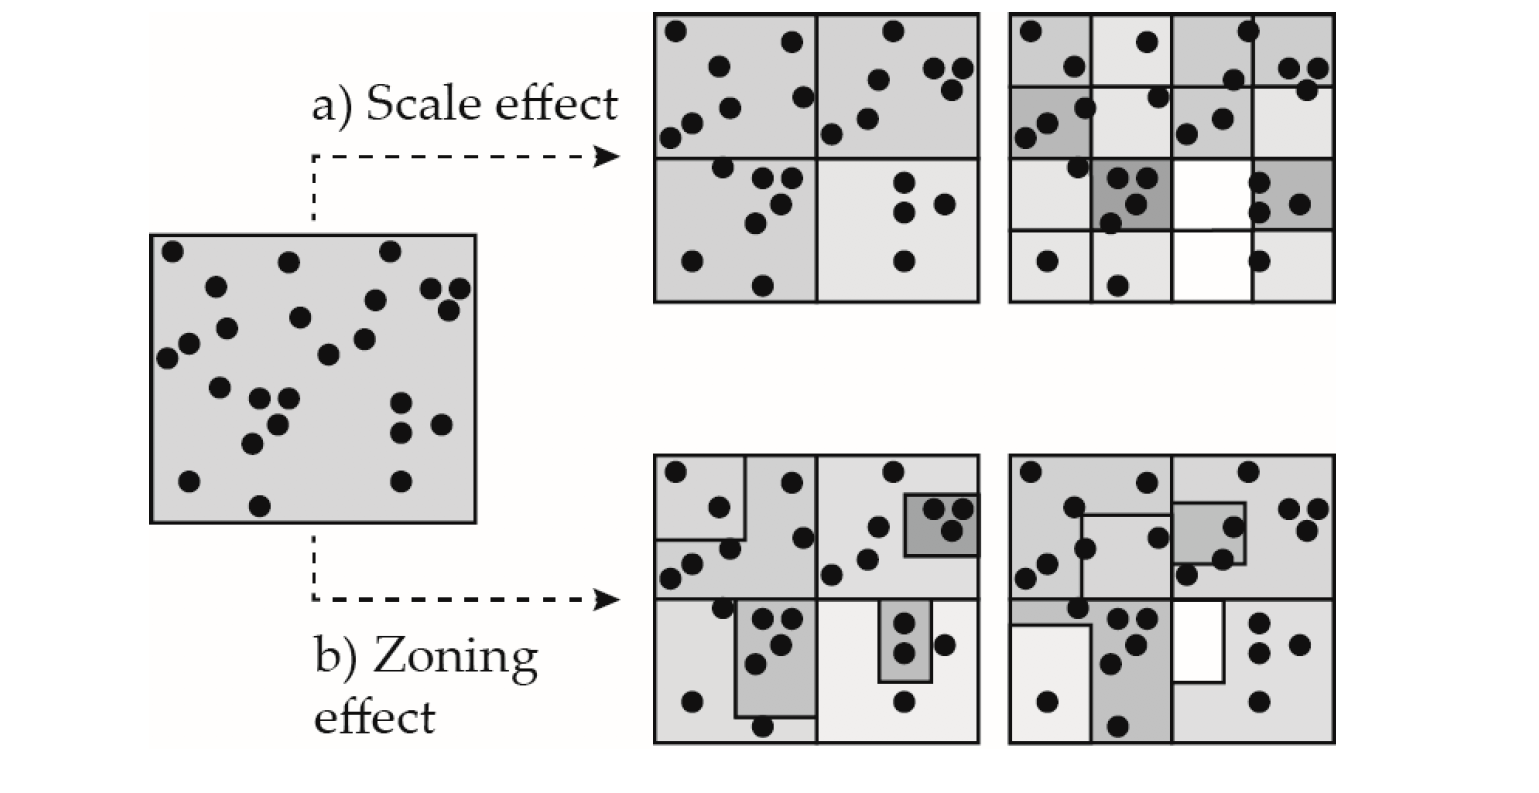
\includegraphics{figs/ch1/maup.png}

}

\caption{Fig. 2. MAUP effect. (a) scale effect; and, (b) zonation
effect. Source: Loidl et al. (2016).}

\end{figure}%

The MAUP is a critical issue as it can impact our analysis and thus any
conclusions we can infer from our results (e.g. A. S. Fotheringham and
Wong 1991). There is no agreed systematic approach on how to handle the
effects of the MAUP. Some have suggested to perform analyses based on
different existing geographical scales, and assess the consistency of
the results and identify potential sources of change. The issue with
such approach is that results from analysis at different scales are
likely to differ because distinct dimensions of a geographic process may
be captured at different scales. For example, in migration studies,
smaller geographies may be more suitable to capture residential mobility
over short distances, while large geographies may be more suitable to
capture long-distance migration. And it is well documented that these
types of moves are driven by different factors. While residential
mobility tends to be driven by housing related reasons, long-distance
migration is more closely related to employment-related motives
(Niedomysl 2011).

An alternative approach is to use the smallest geographical system
available and create random aggregations at various geographical scales,
to directly quantify the extent of scale and zonation. This approach has
shown promising results in applications to study internal migration
flows (Stillwell, Daras, and Bell 2018). Another approach involves the
production of ``meaningful'' or functional geographies that can more
appropriately capture the process of interest. There is an active area
of work defining functional labour markets (Casado-Díaz,
Martínez-Bernabéu, and Rowe 2017), urban areas (Daniel Arribas-Bel,
Garcia-López, and Viladecans-Marsal 2021) and various forms of
geodemographic classifications (A. D. Singleton and Spielman 2013;
Patias, Rowe, and Cavazzi 2019) . However there is the recognition that
none of the existing approaches resolve the effects of the MAUP and
recently it has been suggested that the most plausible `solution' would
be to ignore the MAUP (Wolf et al. 2020).

\subsection{Ecological Fallacy}\label{ecological-fallacy}

Ecological fallacy is an error in the interpretation of statistical data
based on aggregate information. Specifically it refers to inferences
made about the nature of specific individuals based solely on statistics
aggregated for a given group. It is about thinking that relationships
observed for groups necessarily hold for individuals. A key example is
Robinson (1950) who illustrates this problem exploring the difference
between ecological correlations and individual correlations. He looked
at the relationship between country of birth and literacy. Robinson
(1950) used the percent of foreign-born population and percent of
literate population for the 48 states in the United States in 1930. The
ecological correlation based on these data was 0.53. This suggests a
positive association between foreign birth and literacy, and could be
interpreted as foreign born individuals being more likely to be literate
than native-born individuals. Yet, the correlation based on individual
data was negative -0.11 which indicates the opposite. The main point
emerging from this example is to carefully interpret analysis based on
spatial data and avoid making inferences about individuals from these
data.

\subsection{Spatial Dependence}\label{spatial-dependence}

Spatial dependence refers to the spatial relationship of a variable's
values for a pair of locations at a certain distance apart, so that
these values are more similar (or less similar) than expected for
randomly associated pairs of observations (Anselin 1988). For example,
we could think of observed patterns of ethnic segregation in an area are
a result of spillover effects of pre-existing patterns of ethnic
segregation in neighbouring areas. Chapter~\ref{sec-chp5} will
illustrate approach to explicitly incorporate spatial dependence in
regression analysis.

\subsection{Spatial Heterogeneity}\label{spatial-heterogeneity}

Spatial heterogeneity refers to the uneven distribution of a variable's
values across space. Concentration of deprivation or unemployment across
an area are good examples of spatial heterogeneity. We illustrate
various ways to visualise, explore and measure the spatial distribution
of data in multiple chapters. We also discuss on potential modelling
approaches to capture spatial heterogeneity in Chapter~\ref{sec-chp5},
Chapter~\ref{sec-chp7} and Chapter~\ref{sec-chp10}.

\subsection{Spatial nonstationarity}\label{spatial-nonstationarity}

Spatial nonstationarity refers to variations in the relationship between
an outcome variable and a set of predictor variables across space. In a
modelling context, it relates to a situation in which a simple
``global'' model is inappropriate to explain the relationships between a
set of variables. The geographical nature of the model must be modified
to reflect local structural relationships within the data. For example,
ethinic segregation has been positively associated with employment
outcomes in some countries pointing to networks in pre-existing
communities facilitating access to the local labour market. Inversely
ethinic segregation has been negatively associated with employment
outcomes pointing to lack of integration into the broader local
community. We illustrate various modelling approaches to capture spatial
nonstationarity in Chapter~\ref{sec-chp8} and Chapter~\ref{sec-chp9}.

\bookmarksetup{startatroot}

\chapter{Data Wrangling}\label{sec-chp3}

In this chapter, we will cover the fundamentals of the concepts and
functions that you will need to know to navigate this book. We will
introduce key concepts and functions relating to what computational
notebooks are and how they work. We will also cover basic R functions
and data types, including the use of factors. Additionally, we will
offer a basic understanding of the manipulation and mapping of spatial
data frames using commonly used libraries such as \texttt{tidyverse},
\texttt{sf}, \texttt{ggplot} and \texttt{tmap}.

If you are already familiar with R, R computational notebooks and data
types, you may want to jump to Section \hyperref[sec_readdata]{Read
Data} and start from there. This section describes how to read and
manipulate data using \texttt{sf} and \texttt{tidyverse} functions,
including \texttt{mutate()}, \texttt{\%\textgreater{}\%} (known as pipe
operator), \texttt{select()}, \texttt{filter()} and specific packages
and functions how to manipulate spatial data.

The chapter is based on:

\begin{itemize}
\item
  Grolemund and Wickham (2019), this book illustrates key libraries,
  including tidyverse, and functions for data manipulation in R
\item
  Xie, Allaire, and Grolemund (2019), excellent introduction to R
  markdown!
\item
  Williamson (2018), some examples from the first lecture of ENVS450 are
  used to explain the various types of random variables.
\item
  Lovelace, Nowosad, and Muenchow (2019), a really good book on handling
  spatial data and historical background of the evolution of R packages
  for spatial data analysis.
\end{itemize}

\section{Dependencies}\label{dependencies}

This chapter uses the libraries below. Ensure they are installed on your
machine\footnote{You can install package \texttt{mypackage} by running
  the command \texttt{install.packages("mypackage")} on the R prompt or
  through the \texttt{Tools\ -\/-\textgreater{}\ Install\ Packages...}
  menu in RStudio.} before you progress.

\begin{Shaded}
\begin{Highlighting}[]
\CommentTok{\# data manipulation, transformation and visualisation}
\FunctionTok{library}\NormalTok{(tidyverse)}
\CommentTok{\# nice tables}
\FunctionTok{library}\NormalTok{(kableExtra)}
\CommentTok{\# spatial data manipulation}
\FunctionTok{library}\NormalTok{(sf) }
\CommentTok{\# thematic mapping}
\FunctionTok{library}\NormalTok{(tmap) }
\CommentTok{\# colour palettes}
\FunctionTok{library}\NormalTok{(RColorBrewer) }
\FunctionTok{library}\NormalTok{(viridis)}
\end{Highlighting}
\end{Shaded}

\section{Introducing R}\label{introducing-r}

R is a freely available language and environment for statistical
computing and graphics which provides a wide variety of statistical and
graphical techniques. It has gained widespread use in academia and
industry. R offers a wider array of functionality than a traditional
statistics package, such as SPSS and is composed of core (base)
functionality, and is expandable through libraries hosted on
\href{https://cran.r-project.org}{The Comprehensive R Archive Network
(CRAN)}. CRAN is a network of ftp and web servers around the world that
store identical, up-to-date, versions of code and documentation for R.

Commands are sent to R using either the terminal / command line or the R
Console which is installed with R on either Windows or OS X. On Linux,
there is no equivalent of the console, however, third party solutions
exist. On your own machine, R can be installed from
\href{https://www.r-project.org/}{here}.

Normally RStudio is used to implement R coding. RStudio is an integrated
development environment (IDE) for R and provides a more user-friendly
front-end to R than the front-end provided with R.

To run R or RStudio, just double click on the R or RStudio icon.
Throughout this module, we will be using RStudio:

\begin{figure}[H]

{\centering 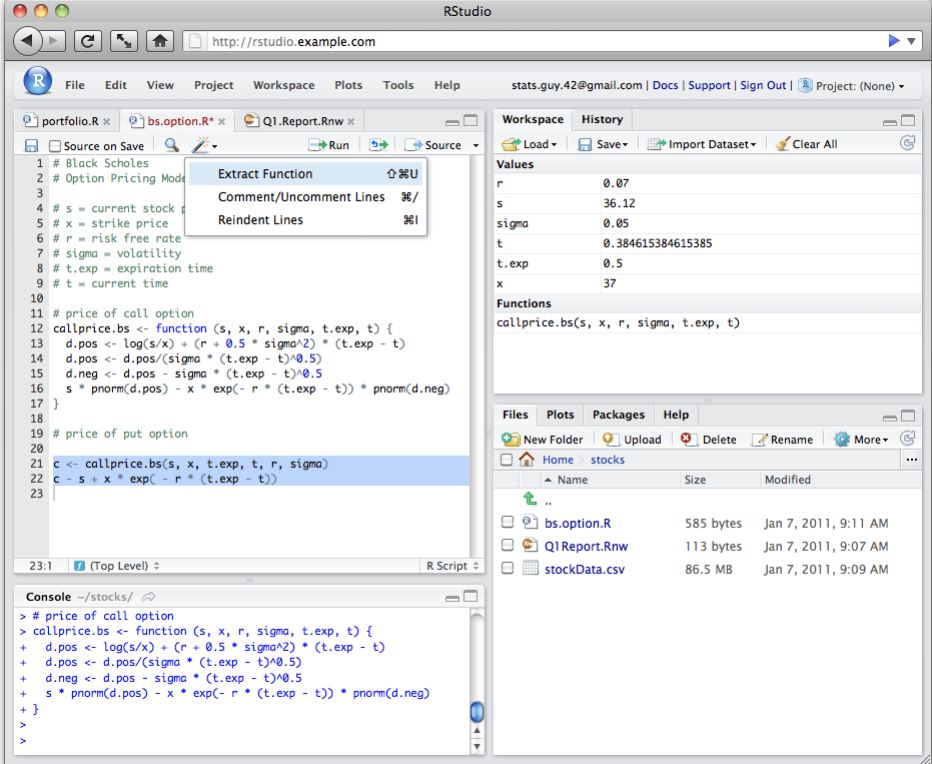
\includegraphics{figs/ch2/rstudio_features.png}

}

\caption{Fig. 1. RStudio features.}

\end{figure}%

If you would like to know more about the various features of RStudio,
watch this \href{https://rstudio.com/products/rstudio/}{video}

\section{Setting the working
directory}\label{setting-the-working-directory}

Before we start any analysis, ensure to set the path to the directory
where we are working. We can easily do that with \texttt{setwd()}.
Please replace in the following line the path to the folder where you
have placed this file -and where the \texttt{data} folder lives.

\begin{Shaded}
\begin{Highlighting}[]
\FunctionTok{setwd}\NormalTok{(}\StringTok{\textquotesingle{}../data/sar.csv\textquotesingle{}}\NormalTok{)}
\FunctionTok{setwd}\NormalTok{(}\StringTok{\textquotesingle{}.\textquotesingle{}}\NormalTok{)}
\end{Highlighting}
\end{Shaded}

\marginnote{\begin{footnotesize}

\begin{tcolorbox}[enhanced jigsaw, title=\textcolor{quarto-callout-note-color}{\faInfo}\hspace{0.5em}{Note}, opacitybacktitle=0.6, arc=.35mm, coltitle=black, colback=white, colbacktitle=quarto-callout-note-color!10!white, toptitle=1mm, colframe=quarto-callout-note-color-frame, leftrule=.75mm, breakable, opacityback=0, bottomrule=.15mm, left=2mm, titlerule=0mm, rightrule=.15mm, toprule=.15mm, bottomtitle=1mm]

It is good practice to not include spaces when naming folders and files.
Use \emph{underscores} or \emph{dots}.

\end{tcolorbox}

\end{footnotesize}}

You can check your current working directory by typing:

\begin{Shaded}
\begin{Highlighting}[]
\FunctionTok{getwd}\NormalTok{()}
\end{Highlighting}
\end{Shaded}

\begin{verbatim}
[1] "/Users/franciscorowe/Dropbox/Francisco/uol/teaching/envs453/202324/san"
\end{verbatim}

\section{R Scripts and Computational
Notebooks}\label{r-scripts-and-computational-notebooks}

An \emph{R script} is a series of commands that you can execute at one
time and help you save time. So you do not repeat the same steps every
time you want to execute the same process with different datasets. An R
script is just a plain text file with R commands in it.

\marginnote{\begin{footnotesize}

\begin{tcolorbox}[enhanced jigsaw, title=\textcolor{quarto-callout-note-color}{\faInfo}\hspace{0.5em}{Note}, opacitybacktitle=0.6, arc=.35mm, coltitle=black, colback=white, colbacktitle=quarto-callout-note-color!10!white, toptitle=1mm, colframe=quarto-callout-note-color-frame, leftrule=.75mm, breakable, opacityback=0, bottomrule=.15mm, left=2mm, titlerule=0mm, rightrule=.15mm, toprule=.15mm, bottomtitle=1mm]

To get familiar with good practices in writing your code in R, we
recommend the \href{https://r4ds.hadley.nz/workflow-basics.html}{Chapter
Workflow: basics} and
\href{https://r4ds.hadley.nz/workflow-scripts}{Workflow: scripts and
projects} from the R in Data Science book by Wickham, Çetinkaya-Rundel,
and Grolemund (2023).

\end{tcolorbox}

\end{footnotesize}}

https://r4ds.hadley.nz/workflow-basics.html

To create an R script in RStudio, you need to

\begin{itemize}
\item
  Open a new script file: \emph{File} \textgreater{} \emph{New File}
  \textgreater{} \emph{R Script}
\item
  Write some code on your new script window by typing eg.
  \texttt{mtcars}
\item
  Run the script. Click anywhere on the line of code, then hit
  \emph{Ctrl + Enter} (Windows) or \emph{Cmd + Enter} (Mac) to run the
  command or select the code chunk and click \emph{run} on the right-top
  corner of your script window. If do that, you should get:
\end{itemize}

\begin{Shaded}
\begin{Highlighting}[]
\NormalTok{mtcars}
\end{Highlighting}
\end{Shaded}

\begin{verbatim}
                     mpg cyl  disp  hp drat    wt  qsec vs am gear carb
Mazda RX4           21.0   6 160.0 110 3.90 2.620 16.46  0  1    4    4
Mazda RX4 Wag       21.0   6 160.0 110 3.90 2.875 17.02  0  1    4    4
Datsun 710          22.8   4 108.0  93 3.85 2.320 18.61  1  1    4    1
Hornet 4 Drive      21.4   6 258.0 110 3.08 3.215 19.44  1  0    3    1
Hornet Sportabout   18.7   8 360.0 175 3.15 3.440 17.02  0  0    3    2
Valiant             18.1   6 225.0 105 2.76 3.460 20.22  1  0    3    1
Duster 360          14.3   8 360.0 245 3.21 3.570 15.84  0  0    3    4
Merc 240D           24.4   4 146.7  62 3.69 3.190 20.00  1  0    4    2
Merc 230            22.8   4 140.8  95 3.92 3.150 22.90  1  0    4    2
Merc 280            19.2   6 167.6 123 3.92 3.440 18.30  1  0    4    4
Merc 280C           17.8   6 167.6 123 3.92 3.440 18.90  1  0    4    4
Merc 450SE          16.4   8 275.8 180 3.07 4.070 17.40  0  0    3    3
Merc 450SL          17.3   8 275.8 180 3.07 3.730 17.60  0  0    3    3
Merc 450SLC         15.2   8 275.8 180 3.07 3.780 18.00  0  0    3    3
Cadillac Fleetwood  10.4   8 472.0 205 2.93 5.250 17.98  0  0    3    4
Lincoln Continental 10.4   8 460.0 215 3.00 5.424 17.82  0  0    3    4
Chrysler Imperial   14.7   8 440.0 230 3.23 5.345 17.42  0  0    3    4
Fiat 128            32.4   4  78.7  66 4.08 2.200 19.47  1  1    4    1
Honda Civic         30.4   4  75.7  52 4.93 1.615 18.52  1  1    4    2
Toyota Corolla      33.9   4  71.1  65 4.22 1.835 19.90  1  1    4    1
Toyota Corona       21.5   4 120.1  97 3.70 2.465 20.01  1  0    3    1
Dodge Challenger    15.5   8 318.0 150 2.76 3.520 16.87  0  0    3    2
AMC Javelin         15.2   8 304.0 150 3.15 3.435 17.30  0  0    3    2
Camaro Z28          13.3   8 350.0 245 3.73 3.840 15.41  0  0    3    4
Pontiac Firebird    19.2   8 400.0 175 3.08 3.845 17.05  0  0    3    2
Fiat X1-9           27.3   4  79.0  66 4.08 1.935 18.90  1  1    4    1
Porsche 914-2       26.0   4 120.3  91 4.43 2.140 16.70  0  1    5    2
Lotus Europa        30.4   4  95.1 113 3.77 1.513 16.90  1  1    5    2
Ford Pantera L      15.8   8 351.0 264 4.22 3.170 14.50  0  1    5    4
Ferrari Dino        19.7   6 145.0 175 3.62 2.770 15.50  0  1    5    6
Maserati Bora       15.0   8 301.0 335 3.54 3.570 14.60  0  1    5    8
Volvo 142E          21.4   4 121.0 109 4.11 2.780 18.60  1  1    4    2
\end{verbatim}

\begin{itemize}
\tightlist
\item
  Save the script: \emph{File} \textgreater{} \emph{Save As}, select
  your required destination folder, and enter any filename that you
  like, provided that it ends with the file extension \emph{.R}
\end{itemize}

An \emph{R Notebook} or a \emph{Quarto Document} are a Markdown options
with descriptive text and code chunks that can be executed independently
and interactively, with output visible immediately beneath a code chunk
- see Xie, Allaire, and Grolemund (2019). A \emph{Quarto Document} is an
improved version of the original \emph{R Notebook}. \emph{Quarto
Document} requires a package called \href{https://quarto.org}{Quarto}.
Quarto does not have a dependency or requirement for R. Quarto is
multilingual, beginning with R, Python, Javascript, and Julia. The
concept is that Quarto will work even for languages that do not yet
exist. This book was original written in \emph{R Notebook} but later
transitioned into \emph{Quarto Documents}.

To create an R Notebook, you need to:

\begin{itemize}
\tightlist
\item
  Open a new script file: \emph{File} \textgreater{} \emph{New File}
  \textgreater{} \emph{R Notebook}
\end{itemize}

\begin{figure}[H]

{\centering 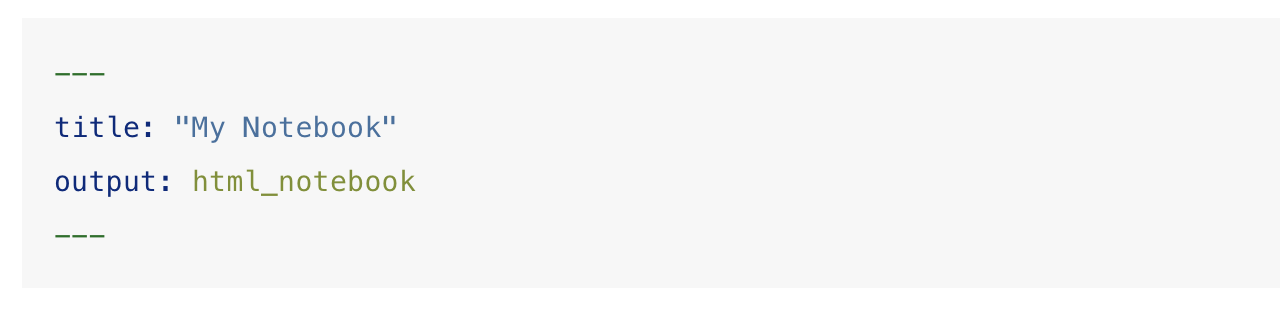
\includegraphics{figs/ch2/rnotebook_yaml.png}

}

\caption{Fig. 2. YAML metadata for notebooks.}

\end{figure}%

\begin{itemize}
\tightlist
\item
  Insert code chunks, either:
\end{itemize}

\begin{enumerate}
\def\labelenumi{\arabic{enumi})}
\tightlist
\item
  use the \emph{Insert} command on the editor toolbar;
\item
  use the keyboard shortcut \emph{Ctrl + Alt + I} or \emph{Cmd + Option
  + I} (Mac); or,
\item
  type the chunk delimiters
  \texttt{\textasciigrave{}\textasciigrave{}\textasciigrave{}\{r\}} and
  \texttt{\textasciigrave{}\textasciigrave{}\textasciigrave{}}
\end{enumerate}

In a chunk code you can produce text output, tables, graphics and write
code! You can control these outputs via chunk options which are provided
inside the curly brackets e.g.:

\begin{figure}[H]

{\centering 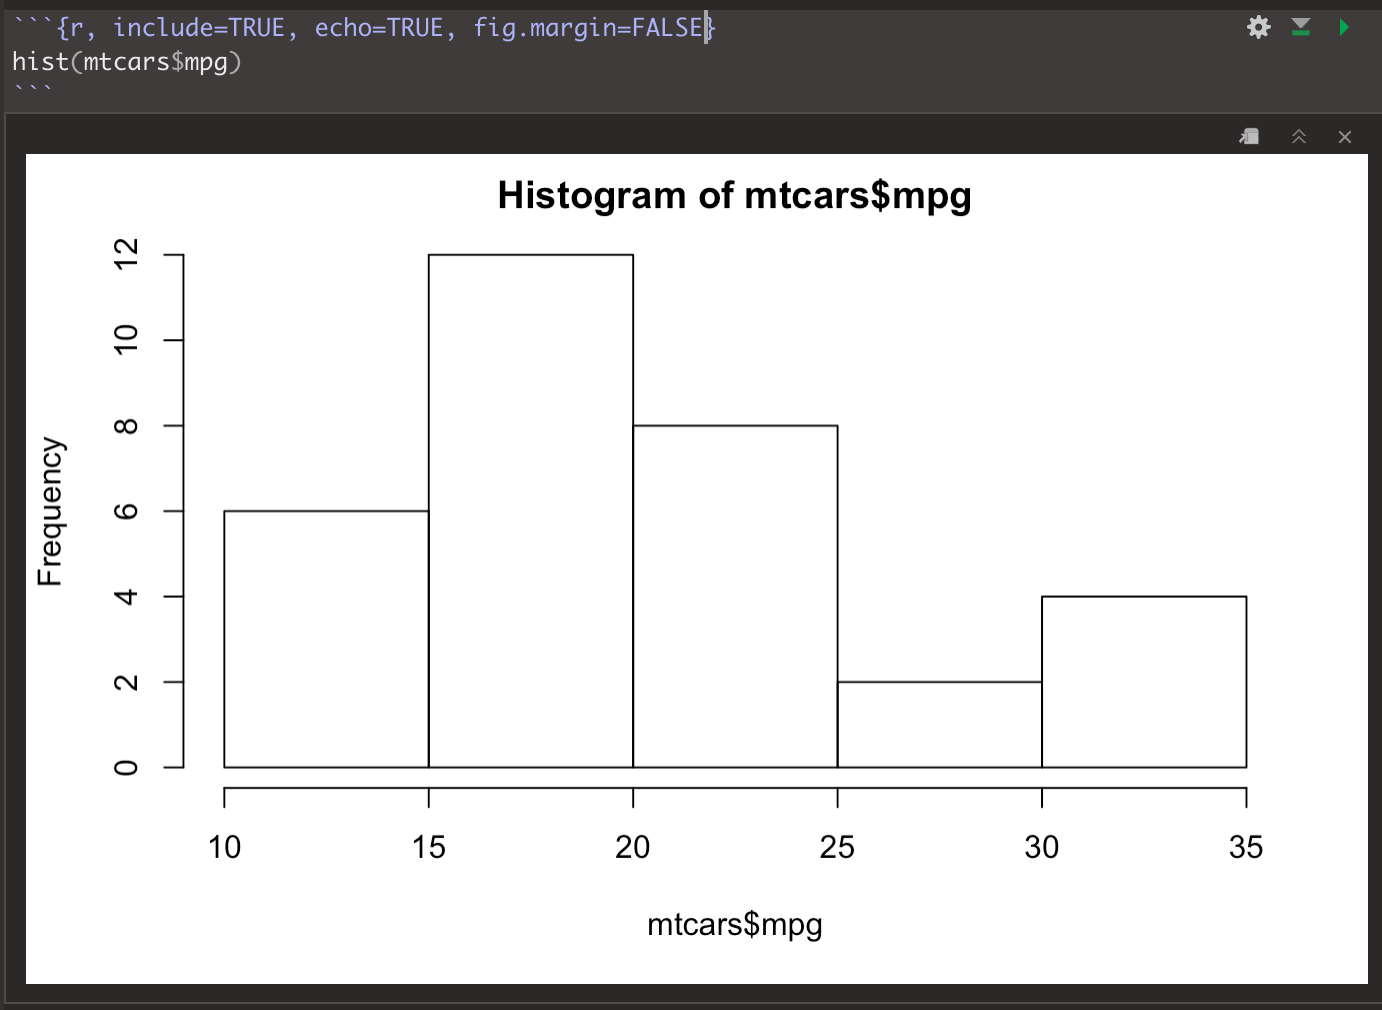
\includegraphics{figs/ch2/codechunk.png}

}

\caption{Fig. 3. Code chunk example. Details on the various options:
https://rmarkdown.rstudio.com/lesson-3.html}

\end{figure}%

\begin{itemize}
\item
  Execute code: hit \emph{``Run Current Chunk''}, \emph{Ctrl + Shift +
  Enter} or \emph{Cmd + Shift + Enter} (Mac)
\item
  Save an R notebook: \emph{File} \textgreater{} \emph{Save As}. A
  notebook has a \texttt{*.Rmd} extension and when it is saved a
  \texttt{*.nb.html} file is automatically created. The latter is a
  self-contained HTML file which contains both a rendered copy of the
  notebook with all current chunk outputs and a copy of the *.Rmd file
  itself.
\end{itemize}

Rstudio also offers a \emph{Preview} option on the toolbar which can be
used to create pdf, html and word versions of the notebook. To do this,
choose from the drop-down list menu \texttt{knit\ to\ ...}

To create a \emph{Quarto Document}, you need to:

\begin{itemize}
\tightlist
\item
  Open a new script file: \emph{File} \textgreater{} \emph{New File}
  \textgreater{} \emph{Quarto Document}
\end{itemize}

Quarto Documents work in the same way as R Notebooks with small
variations. You find a comprehensive guide on the
\href{https://quarto.org/docs/guide/}{Quarto website}.

\section{Getting Help}\label{getting-help}

You can use \texttt{help} or \texttt{?} to ask for details for a
specific function:

\begin{Shaded}
\begin{Highlighting}[]
\FunctionTok{help}\NormalTok{(sqrt) }\CommentTok{\#or}
\NormalTok{?sqrt}
\end{Highlighting}
\end{Shaded}

And using \texttt{example} provides examples for said function:

\begin{Shaded}
\begin{Highlighting}[]
\FunctionTok{example}\NormalTok{(sqrt)}
\end{Highlighting}
\end{Shaded}

\begin{verbatim}

sqrt> require(stats) # for spline

sqrt> require(graphics)

sqrt> xx <- -9:9

sqrt> plot(xx, sqrt(abs(xx)),  col = "red")
\end{verbatim}

\includegraphics{03-data-wrangling_files/figure-pdf/unnamed-chunk-8-1.pdf}

\begin{verbatim}

sqrt> lines(spline(xx, sqrt(abs(xx)), n=101), col = "pink")
\end{verbatim}

\section{Variables and objects}\label{variables-and-objects}

An \emph{object} is a data structure having attributes and methods. In
fact, everything in R is an object!

A \emph{variable} is a type of data object. Data objects also include
list, vector, matrices and text.

\begin{itemize}
\tightlist
\item
  Creating a data object
\end{itemize}

In R a variable can be created by using the symbol \texttt{\textless{}-}
to assign a value to a variable name. The variable name is entered on
the left \texttt{\textless{}-} and the value on the right. Note: Data
objects can be given any name, provided that they start with a letter of
the alphabet, and include only letters of the alphabet, numbers and the
characters \texttt{.} and \texttt{\_}. Hence AgeGroup, Age\_Group and
Age.Group are all valid names for an R data object. Note also that R is
case-sensitive, to agegroup and AgeGroup would be treated as different
data objects.

To save the value \emph{28} to a variable (data object) labelled
\emph{age}, run the code:

\begin{Shaded}
\begin{Highlighting}[]
\NormalTok{age }\OtherTok{\textless{}{-}} \DecValTok{28}
\end{Highlighting}
\end{Shaded}

\begin{itemize}
\tightlist
\item
  Inspecting a data object
\end{itemize}

To inspect the contents of the data object \emph{age} run the following
line of code:

\begin{Shaded}
\begin{Highlighting}[]
\NormalTok{age}
\end{Highlighting}
\end{Shaded}

\begin{verbatim}
[1] 28
\end{verbatim}

Find out what kind (class) of data object \emph{age} is using:

\begin{Shaded}
\begin{Highlighting}[]
\FunctionTok{class}\NormalTok{(age) }
\end{Highlighting}
\end{Shaded}

\begin{verbatim}
[1] "numeric"
\end{verbatim}

Inspect the structure of the \emph{age} data object:

\begin{Shaded}
\begin{Highlighting}[]
\FunctionTok{str}\NormalTok{(age) }
\end{Highlighting}
\end{Shaded}

\begin{verbatim}
 num 28
\end{verbatim}

\begin{itemize}
\tightlist
\item
  The \emph{vector} data object
\end{itemize}

What if we have more than one response? We can use the \texttt{c(\ )}
function to combine multiple values into one data vector object:

\begin{Shaded}
\begin{Highlighting}[]
\NormalTok{age }\OtherTok{\textless{}{-}} \FunctionTok{c}\NormalTok{(}\DecValTok{28}\NormalTok{, }\DecValTok{36}\NormalTok{, }\DecValTok{25}\NormalTok{, }\DecValTok{24}\NormalTok{, }\DecValTok{32}\NormalTok{)}
\NormalTok{age}
\end{Highlighting}
\end{Shaded}

\begin{verbatim}
[1] 28 36 25 24 32
\end{verbatim}

\begin{Shaded}
\begin{Highlighting}[]
\FunctionTok{class}\NormalTok{(age) }\CommentTok{\#Still numeric..}
\end{Highlighting}
\end{Shaded}

\begin{verbatim}
[1] "numeric"
\end{verbatim}

\begin{Shaded}
\begin{Highlighting}[]
\FunctionTok{str}\NormalTok{(age) }\CommentTok{\#..but now a vector (set) of 5 separate values}
\end{Highlighting}
\end{Shaded}

\begin{verbatim}
 num [1:5] 28 36 25 24 32
\end{verbatim}

Note that on each line in the code above any text following the
\texttt{\#} character is ignored by R when executing the code. Instead,
text following a \texttt{\#} can be used to add comments to the code to
make clear what the code is doing. Two marks of good code are a clear
layout and clear commentary on the code.

\subsection{Basic Data Types}\label{basic-data-types}

There are a number of data types. Four are the most common. In R,
\textbf{numeric} is the default type for numbers. It stores all numbers
as floating-point numbers (numbers with decimals). This is because most
statistical calculations deal with numbers with up to two decimals.

\begin{itemize}
\tightlist
\item
  Numeric
\end{itemize}

\begin{Shaded}
\begin{Highlighting}[]
\NormalTok{num }\OtherTok{\textless{}{-}} \FloatTok{4.5} \CommentTok{\# Decimal values}
\FunctionTok{class}\NormalTok{(num)}
\end{Highlighting}
\end{Shaded}

\begin{verbatim}
[1] "numeric"
\end{verbatim}

\begin{itemize}
\tightlist
\item
  Integer
\end{itemize}

\begin{Shaded}
\begin{Highlighting}[]
\NormalTok{int }\OtherTok{\textless{}{-}} \FunctionTok{as.integer}\NormalTok{(}\DecValTok{4}\NormalTok{) }\CommentTok{\# Natural numbers. Note integers are also numerics.}
\FunctionTok{class}\NormalTok{(int)}
\end{Highlighting}
\end{Shaded}

\begin{verbatim}
[1] "integer"
\end{verbatim}

\begin{itemize}
\tightlist
\item
  Character
\end{itemize}

\begin{Shaded}
\begin{Highlighting}[]
\NormalTok{cha }\OtherTok{\textless{}{-}} \StringTok{"are you enjoying this?"} \CommentTok{\# text or string. You can also type \textasciigrave{}as.character("are you enjoying this?")\textasciigrave{}}
\FunctionTok{class}\NormalTok{(cha)}
\end{Highlighting}
\end{Shaded}

\begin{verbatim}
[1] "character"
\end{verbatim}

\begin{itemize}
\tightlist
\item
  Logical
\end{itemize}

\begin{Shaded}
\begin{Highlighting}[]
\NormalTok{log }\OtherTok{\textless{}{-}} \DecValTok{2} \SpecialCharTok{\textless{}} \DecValTok{1} \CommentTok{\# assigns TRUE or FALSE. In this case, FALSE as 2 is greater than 1}
\NormalTok{log}
\end{Highlighting}
\end{Shaded}

\begin{verbatim}
[1] FALSE
\end{verbatim}

\begin{Shaded}
\begin{Highlighting}[]
\FunctionTok{class}\NormalTok{(log)}
\end{Highlighting}
\end{Shaded}

\begin{verbatim}
[1] "logical"
\end{verbatim}

\subsection{Random Variables}\label{random-variables}

In statistics, we differentiate between data to capture:

\begin{itemize}
\item
  \emph{Qualitative attributes} categorise objects eg.gender, marital
  status. To measure these attributes, we use \emph{Categorical} data
  which can be divided into:

  \begin{itemize}
  \tightlist
  \item
    \emph{Nominal} data in categories that have no inherent order eg.
    gender
  \item
    \emph{Ordinal} data in categories that have an inherent order eg.
    income bands
  \end{itemize}
\item
  \emph{Quantitative attributes}:

  \begin{itemize}
  \tightlist
  \item
    \emph{Discrete} data: count objects of a certain category eg. number
    of kids, cars
  \item
    \emph{Continuous} data: precise numeric measures eg. weight, income,
    length.
  \end{itemize}
\end{itemize}

In R these three types of random variables are represented by the
following types of R data object:

\begin{longtable}[]{@{}ll@{}}
\toprule\noalign{}
variables & objects \\
\midrule\noalign{}
\endhead
\bottomrule\noalign{}
\endlastfoot
nominal & factor \\
ordinal & ordered factor \\
discrete & numeric \\
continuous & numeric \\
\end{longtable}

We have already encountered the R data type \emph{numeric}. The next
section introduces the \emph{factor} data type.

\subsubsection{Factor}\label{factor}

\textbf{What is a factor?}

A factor variable assigns a numeric code to each possible category
(\emph{level}) in a variable. Behind the scenes, R stores the variable
using these numeric codes to save space and speed up computing. For
example, compare the size of a list of 10,000 \emph{males} and
\emph{females} to a list of 10,000 1s and 0s. At the same time R also
saves the category names associated with each numeric code (level).
These are used for display purposes.

For example, the variable \emph{gender}, converted to a factor, would be
stored as a series of 1s and 2s, where 1 = female and 2 = male; but
would be displayed in all outputs using their category labels of
\emph{female} and \emph{male}.

\textbf{Creating a factor}

To convert a numeric or character vector into a factor use the
\texttt{factor(\ )} function. For instance:

\begin{Shaded}
\begin{Highlighting}[]
\NormalTok{gender }\OtherTok{\textless{}{-}} \FunctionTok{c}\NormalTok{(}\StringTok{"female"}\NormalTok{,}\StringTok{"male"}\NormalTok{,}\StringTok{"male"}\NormalTok{,}\StringTok{"female"}\NormalTok{,}\StringTok{"female"}\NormalTok{) }\CommentTok{\# create a gender variable}
\NormalTok{gender }\OtherTok{\textless{}{-}} \FunctionTok{factor}\NormalTok{(gender) }\CommentTok{\# replace character vector with a factor version}
\NormalTok{gender}
\end{Highlighting}
\end{Shaded}

\begin{verbatim}
[1] female male   male   female female
Levels: female male
\end{verbatim}

\begin{Shaded}
\begin{Highlighting}[]
\FunctionTok{class}\NormalTok{(gender)}
\end{Highlighting}
\end{Shaded}

\begin{verbatim}
[1] "factor"
\end{verbatim}

\begin{Shaded}
\begin{Highlighting}[]
\FunctionTok{str}\NormalTok{(gender)}
\end{Highlighting}
\end{Shaded}

\begin{verbatim}
 Factor w/ 2 levels "female","male": 1 2 2 1 1
\end{verbatim}

Now \emph{gender} is a factor and is stored as a series of 1s and 2s,
with 1s representing females and 2s representing males. The function
\texttt{levels(\ )} lists the levels (categories) associated with a
given factor variable:

\begin{Shaded}
\begin{Highlighting}[]
\FunctionTok{levels}\NormalTok{(gender)}
\end{Highlighting}
\end{Shaded}

\begin{verbatim}
[1] "female" "male"  
\end{verbatim}

The categories are reported in the order that they have been numbered
(starting from 1). Hence from the output we can infer that females are
coded as 1, and males as 2.

\section{Data Frames}\label{data-frames}

R stores different types of data using different types of data
structure. Data are normally stored as a \emph{data.frame}. A data
frames contain one row per observation (e.g.~wards) and one column per
attribute (eg. population and health).

We create three variables wards, population (\texttt{pop}) and people
with good health (\texttt{ghealth}). We use 2011 census data counts for
total population and good health for wards in Liverpool.

\begin{Shaded}
\begin{Highlighting}[]
\NormalTok{wards }\OtherTok{\textless{}{-}} \FunctionTok{c}\NormalTok{(}\StringTok{"Allerton and Hunts Cross"}\NormalTok{,}\StringTok{"Anfield"}\NormalTok{,}\StringTok{"Belle Vale"}\NormalTok{,}\StringTok{"Central"}\NormalTok{,}\StringTok{"Childwall"}\NormalTok{,}\StringTok{"Church"}\NormalTok{,}\StringTok{"Clubmoor"}\NormalTok{,}\StringTok{"County"}\NormalTok{,}\StringTok{"Cressington"}\NormalTok{,}\StringTok{"Croxteth"}\NormalTok{,}\StringTok{"Everton"}\NormalTok{,}\StringTok{"Fazakerley"}\NormalTok{,}\StringTok{"Greenbank"}\NormalTok{,}\StringTok{"Kensington and Fairfield"}\NormalTok{,}\StringTok{"Kirkdale"}\NormalTok{,}\StringTok{"Knotty Ash"}\NormalTok{,}\StringTok{"Mossley Hill"}\NormalTok{,}\StringTok{"Norris Green"}\NormalTok{,}\StringTok{"Old Swan"}\NormalTok{,}\StringTok{"Picton"}\NormalTok{,}\StringTok{"Princes Park"}\NormalTok{,}\StringTok{"Riverside"}\NormalTok{,}\StringTok{"St Michael\textquotesingle{}s"}\NormalTok{,}\StringTok{"Speke{-}Garston"}\NormalTok{,}\StringTok{"Tuebrook and Stoneycroft"}\NormalTok{,}\StringTok{"Warbreck"}\NormalTok{,}\StringTok{"Wavertree"}\NormalTok{,}\StringTok{"West Derby"}\NormalTok{,}\StringTok{"Woolton"}\NormalTok{,}\StringTok{"Yew Tree"}\NormalTok{)}

\NormalTok{pop }\OtherTok{\textless{}{-}} \FunctionTok{c}\NormalTok{(}\DecValTok{14853}\NormalTok{,}\DecValTok{14510}\NormalTok{,}\DecValTok{15004}\NormalTok{,}\DecValTok{20340}\NormalTok{,}\DecValTok{13908}\NormalTok{,}\DecValTok{13974}\NormalTok{,}\DecValTok{15272}\NormalTok{,}\DecValTok{14045}\NormalTok{,}\DecValTok{14503}\NormalTok{,}
                \DecValTok{14561}\NormalTok{,}\DecValTok{14782}\NormalTok{,}\DecValTok{16786}\NormalTok{,}\DecValTok{16132}\NormalTok{,}\DecValTok{15377}\NormalTok{,}\DecValTok{16115}\NormalTok{,}\DecValTok{13312}\NormalTok{,}\DecValTok{13816}\NormalTok{,}\DecValTok{15047}\NormalTok{,}
                \DecValTok{16461}\NormalTok{,}\DecValTok{17009}\NormalTok{,}\DecValTok{17104}\NormalTok{,}\DecValTok{18422}\NormalTok{,}\DecValTok{12991}\NormalTok{,}\DecValTok{20300}\NormalTok{,}\DecValTok{16489}\NormalTok{,}\DecValTok{16481}\NormalTok{,}\DecValTok{14772}\NormalTok{,}
                \DecValTok{14382}\NormalTok{,}\DecValTok{12921}\NormalTok{,}\DecValTok{16746}\NormalTok{)}

\NormalTok{ghealth }\OtherTok{\textless{}{-}} \FunctionTok{c}\NormalTok{(}\DecValTok{7274}\NormalTok{,}\DecValTok{6124}\NormalTok{,}\DecValTok{6129}\NormalTok{,}\DecValTok{11925}\NormalTok{,}\DecValTok{7219}\NormalTok{,}\DecValTok{7461}\NormalTok{,}\DecValTok{6403}\NormalTok{,}\DecValTok{5930}\NormalTok{,}\DecValTok{7094}\NormalTok{,}\DecValTok{6992}\NormalTok{,}
                 \DecValTok{5517}\NormalTok{,}\DecValTok{7879}\NormalTok{,}\DecValTok{8990}\NormalTok{,}\DecValTok{6495}\NormalTok{,}\DecValTok{6662}\NormalTok{,}\DecValTok{5981}\NormalTok{,}\DecValTok{7322}\NormalTok{,}\DecValTok{6529}\NormalTok{,}\DecValTok{7192}\NormalTok{,}\DecValTok{7953}\NormalTok{,}
                 \DecValTok{7636}\NormalTok{,}\DecValTok{9001}\NormalTok{,}\DecValTok{6450}\NormalTok{,}\DecValTok{8973}\NormalTok{,}\DecValTok{7302}\NormalTok{,}\DecValTok{7521}\NormalTok{,}\DecValTok{7268}\NormalTok{,}\DecValTok{7013}\NormalTok{,}\DecValTok{6025}\NormalTok{,}\DecValTok{7717}\NormalTok{)}
\end{Highlighting}
\end{Shaded}

Note that \texttt{pop} and \texttt{ghealth} and \texttt{wards} contains
characters.

\subsection{Creating A Data Frame}\label{creating-a-data-frame}

We can create a data frame and examine its structure:

\begin{Shaded}
\begin{Highlighting}[]
\NormalTok{df }\OtherTok{\textless{}{-}} \FunctionTok{data.frame}\NormalTok{(wards, pop, ghealth)}
\NormalTok{df }\CommentTok{\# or use view(data)}
\end{Highlighting}
\end{Shaded}

\begin{verbatim}
                      wards   pop ghealth
1  Allerton and Hunts Cross 14853    7274
2                   Anfield 14510    6124
3                Belle Vale 15004    6129
4                   Central 20340   11925
5                 Childwall 13908    7219
6                    Church 13974    7461
7                  Clubmoor 15272    6403
8                    County 14045    5930
9               Cressington 14503    7094
10                 Croxteth 14561    6992
11                  Everton 14782    5517
12               Fazakerley 16786    7879
13                Greenbank 16132    8990
14 Kensington and Fairfield 15377    6495
15                 Kirkdale 16115    6662
16               Knotty Ash 13312    5981
17             Mossley Hill 13816    7322
18             Norris Green 15047    6529
19                 Old Swan 16461    7192
20                   Picton 17009    7953
21             Princes Park 17104    7636
22                Riverside 18422    9001
23             St Michael's 12991    6450
24            Speke-Garston 20300    8973
25 Tuebrook and Stoneycroft 16489    7302
26                 Warbreck 16481    7521
27                Wavertree 14772    7268
28               West Derby 14382    7013
29                  Woolton 12921    6025
30                 Yew Tree 16746    7717
\end{verbatim}

\begin{Shaded}
\begin{Highlighting}[]
\FunctionTok{str}\NormalTok{(df) }\CommentTok{\# or use glimpse(data) }
\end{Highlighting}
\end{Shaded}

\begin{verbatim}
'data.frame':   30 obs. of  3 variables:
 $ wards  : chr  "Allerton and Hunts Cross" "Anfield" "Belle Vale" "Central" ...
 $ pop    : num  14853 14510 15004 20340 13908 ...
 $ ghealth: num  7274 6124 6129 11925 7219 ...
\end{verbatim}

\subsection{Referencing Data Frames}\label{referencing-data-frames}

To refer to particular parts of a dataframe - say, a particular column
(an area attribute), or a subset of respondents. Hence it is worth
spending some time understanding how to reference dataframes.

The relevant R function, \texttt{{[}\ {]}}, has the format
\texttt{{[}row,col{]}} or, more generally,
\texttt{{[}set\ of\ rows,\ set\ of\ cols{]}}.

Run the following commands to get a feel of how to extract different
slices of the data:

\begin{Shaded}
\begin{Highlighting}[]
\NormalTok{df }\CommentTok{\# whole data.frame}
\NormalTok{df[}\DecValTok{1}\NormalTok{, }\DecValTok{1}\NormalTok{] }\CommentTok{\# contents of first row and column}
\NormalTok{df[}\DecValTok{2}\NormalTok{, }\DecValTok{2}\SpecialCharTok{:}\DecValTok{3}\NormalTok{] }\CommentTok{\# contents of the second row, second and third columns}
\NormalTok{df[}\DecValTok{1}\NormalTok{, ] }\CommentTok{\# first row, ALL columns [the default if no columns specified]}
\NormalTok{df[ ,}\DecValTok{1}\SpecialCharTok{:}\DecValTok{2}\NormalTok{] }\CommentTok{\# ALL rows; first and second columns}
\NormalTok{df[}\FunctionTok{c}\NormalTok{(}\DecValTok{1}\NormalTok{,}\DecValTok{3}\NormalTok{,}\DecValTok{5}\NormalTok{), ] }\CommentTok{\# rows 1,3,5; ALL columns}
\NormalTok{df[ , }\DecValTok{2}\NormalTok{] }\CommentTok{\# ALL rows; second column (by default results containing only }
             \CommentTok{\#one column are converted back into a vector)}
\NormalTok{df[ , }\DecValTok{2}\NormalTok{, drop}\OtherTok{=}\ConstantTok{FALSE}\NormalTok{] }\CommentTok{\# ALL rows; second column (returned as a data.frame)}
\end{Highlighting}
\end{Shaded}

In the above, note that we have used two other R functions:

\begin{itemize}
\item
  \texttt{1:3} The colon operator tells R to produce a list of numbers
  including the named start and end points.
\item
  \texttt{c(1,3,5)} Tells R to combine the contents within the brackets
  into one list of objects
\end{itemize}

Run both of these fuctions on their own to get a better understanding of
what they do.

Three other methods for referencing the contents of a data.frame make
direct use of the variable names within the data.frame, which tends to
make for easier to read/understand code:

\begin{Shaded}
\begin{Highlighting}[]
\NormalTok{df[,}\StringTok{"pop"}\NormalTok{] }\CommentTok{\# variable name in quotes inside the square brackets}
\NormalTok{df}\SpecialCharTok{$}\NormalTok{pop }\CommentTok{\# variable name prefixed with $ and appended to the data.frame name}
\CommentTok{\# or you can use attach}
\FunctionTok{attach}\NormalTok{(df)}
\NormalTok{pop }\CommentTok{\# but be careful if you already have an age variable in your local workspace}
\end{Highlighting}
\end{Shaded}

Want to check the variables available, use the \texttt{names(\ )}:

\begin{Shaded}
\begin{Highlighting}[]
\FunctionTok{names}\NormalTok{(df)}
\end{Highlighting}
\end{Shaded}

\begin{verbatim}
[1] "wards"   "pop"     "ghealth"
\end{verbatim}

\section{Read Data}\label{sec_readdata}

Ensure your memory is clear

\begin{Shaded}
\begin{Highlighting}[]
\FunctionTok{rm}\NormalTok{(}\AttributeTok{list=}\FunctionTok{ls}\NormalTok{()) }\CommentTok{\# rm for targeted deletion / ls for listing all existing objects}
\end{Highlighting}
\end{Shaded}

\marginnote{\begin{footnotesize}

\begin{tcolorbox}[enhanced jigsaw, title=\textcolor{quarto-callout-note-color}{\faInfo}\hspace{0.5em}{Note}, opacitybacktitle=0.6, arc=.35mm, coltitle=black, colback=white, colbacktitle=quarto-callout-note-color!10!white, toptitle=1mm, colframe=quarto-callout-note-color-frame, leftrule=.75mm, breakable, opacityback=0, bottomrule=.15mm, left=2mm, titlerule=0mm, rightrule=.15mm, toprule=.15mm, bottomtitle=1mm]

When opening a file, ensure the correct directory set up pointing to
your data. It may differ from your existing working directory.

\end{tcolorbox}

\end{footnotesize}}

There are many commands to read / load data onto R. The command to use
will depend upon the format they have been saved. Normally they are
saved in \emph{csv} format from Excel or other software packages. So we
use either:

\begin{itemize}
\tightlist
\item
  \texttt{df\ \textless{}-\ read.table("path/file\_name.csv",\ header\ =\ FALSE,\ sep\ =",")}
\item
  \texttt{df\ \textless{}-\ read("path/file\_name.csv",\ header\ =\ FALSE)}
\item
  \texttt{df\ \textless{}-\ read.csv2("path/file\_name.csv",\ header\ =\ FALSE)}
\end{itemize}

To read files in other formats, refer to this useful
\href{https://www.datacamp.com/community/tutorials/r-data-import-tutorial?utm_source=adwords_ppc&utm_campaignid=1655852085&utm_adgroupid=61045434382&utm_device=c&utm_keyword=\%2Bread\%20\%2Bdata\%20\%2Br&utm_matchtype=b&utm_network=g&utm_adpostion=1t1&utm_creative=318880582308&utm_targetid=kwd-309793905111&utm_loc_interest_ms=&utm_loc_physical_ms=9046551&gclid=CjwKCAiA3uDwBRBFEiwA1VsajJO0QK0Jg7VipIt8_t82qQrnUliI0syAlh8CIxnE76Rb0kh3FbiehxoCzCgQAvD_BwE\#csv}{DataCamp
tutorial}

\begin{Shaded}
\begin{Highlighting}[]
\NormalTok{census }\OtherTok{\textless{}{-}} \FunctionTok{read.csv}\NormalTok{(}\StringTok{"data/census/census\_data.csv"}\NormalTok{)}
\FunctionTok{head}\NormalTok{(census)}
\end{Highlighting}
\end{Shaded}

\begin{verbatim}
       code                     ward pop16_74 higher_managerial   pop ghealth
1 E05000886 Allerton and Hunts Cross    10930              1103 14853    7274
2 E05000887                  Anfield    10712               312 14510    6124
3 E05000888               Belle Vale    10987               432 15004    6129
4 E05000889                  Central    19174              1346 20340   11925
5 E05000890                Childwall    10410              1123 13908    7219
6 E05000891                   Church    10569              1843 13974    7461
\end{verbatim}

\subsection{Quickly inspect the data}\label{quickly-inspect-the-data}

Using the following questions to lead the inspection: What class? What R
data types? What data types?

\begin{Shaded}
\begin{Highlighting}[]
\CommentTok{\# 1}
\FunctionTok{class}\NormalTok{(census)}
\CommentTok{\# 2 \& 3}
\FunctionTok{str}\NormalTok{(census)}
\end{Highlighting}
\end{Shaded}

Just interested in the variable names:

\begin{Shaded}
\begin{Highlighting}[]
\FunctionTok{names}\NormalTok{(census)}
\end{Highlighting}
\end{Shaded}

\begin{verbatim}
[1] "code"              "ward"              "pop16_74"         
[4] "higher_managerial" "pop"               "ghealth"          
\end{verbatim}

or want to view the data:

\texttt{View(census)}

\section{Manipulation Data}\label{manipulation-data}

\subsection{Adding New Variables}\label{adding-new-variables}

Usually you want to add / create new variables to your data frame using
existing variables eg. computing percentages by dividing two variables.
There are many ways in which you can do this i.e.~referecing a data
frame as we have done above, or using \texttt{\$}
(e.g.~\texttt{census\$pop}). For this module, we'll use
\texttt{tidyverse}:

\begin{Shaded}
\begin{Highlighting}[]
\NormalTok{census }\OtherTok{\textless{}{-}}\NormalTok{ census }\SpecialCharTok{\%\textgreater{}\%} 
  \FunctionTok{mutate}\NormalTok{( }\AttributeTok{per\_ghealth =}\NormalTok{ ghealth }\SpecialCharTok{/}\NormalTok{ pop )}
\end{Highlighting}
\end{Shaded}

Note we used a \emph{pipe operator} \texttt{\%\textgreater{}\%}, which
helps make the code more efficient and readable - more details, see
Grolemund and Wickham (2019). When using the pipe operator, recall to
first indicate the data frame before \texttt{\%\textgreater{}\%}.

Note also the use a variable name before the \texttt{=} sign in brackets
to indicate the name of the new variable after \texttt{mutate}.

\subsection{Selecting Variables}\label{selecting-variables}

Usually you want to select a subset of variables for your analysis as
storing to large data sets in your R memory can reduce the processing
speed of your machine. A selection of data can be achieved by using the
\texttt{select} function:

\begin{Shaded}
\begin{Highlighting}[]
\NormalTok{ndf }\OtherTok{\textless{}{-}}\NormalTok{ census }\SpecialCharTok{\%\textgreater{}\%} 
  \FunctionTok{select}\NormalTok{( ward, pop16\_74, per\_ghealth )}
\end{Highlighting}
\end{Shaded}

Again first indicate the data frame and then the variable you want to
select to build a new data frame. Note the code chunk above has created
a new data frame called \texttt{ndf}. Explore it.

\subsection{Filtering Data}\label{filtering-data}

You may also want to filter values based on defined conditions. You may
want to filter observations greater than a certain threshold or only
areas within a certain region. For example, you may want to select areas
with a percentage of good health population over 50\%:

\begin{Shaded}
\begin{Highlighting}[]
\NormalTok{ndf2 }\OtherTok{\textless{}{-}}\NormalTok{ census }\SpecialCharTok{\%\textgreater{}\%} 
  \FunctionTok{filter}\NormalTok{( per\_ghealth }\SpecialCharTok{\textless{}} \FloatTok{0.5}\NormalTok{ )}
\end{Highlighting}
\end{Shaded}

You can use more than one variables to set conditions. Use
``\texttt{,}'' to add a condition.

\subsection{Joining Data Drames}\label{joining-data-drames}

When working with spatial data, we often need to join data. To this end,
you need a common unique \texttt{id\ variable}. Let's say, we want to
add a data frame containing census data on households for Liverpool, and
join the new attributes to one of the existing data frames in the
workspace. First we will read the data frame we want to join
(i.e.~\texttt{census\_data2.csv}).

\begin{Shaded}
\begin{Highlighting}[]
\CommentTok{\# read data}
\NormalTok{census2 }\OtherTok{\textless{}{-}} \FunctionTok{read.csv}\NormalTok{(}\StringTok{"data/census/census\_data2.csv"}\NormalTok{)}
\CommentTok{\# visualise data structure}
\FunctionTok{str}\NormalTok{(census2)}
\end{Highlighting}
\end{Shaded}

\begin{verbatim}
'data.frame':   30 obs. of  3 variables:
 $ geo_code               : chr  "E05000886" "E05000887" "E05000888" "E05000889" ...
 $ households             : int  6359 6622 6622 7139 5391 5884 6576 6745 6317 6024 ...
 $ socialrented_households: int  827 1508 2818 1311 374 178 2859 1564 1023 1558 ...
\end{verbatim}

The variable \texttt{geo\_code} in this data frame corresponds to the
\texttt{code} in the existing data frame and they are unique so they can
be automatically matched by using the \texttt{merge()} function. The
\texttt{merge()} function uses two arguments: \texttt{x} and \texttt{y}.
The former refers to data frame 1 and the latter to data frame 2. Both
of these two data frames must have a \texttt{id} variable containing the
same information. Note they can have different names. Another key
argument to include is \texttt{all.x=TRUE} which tells the function to
keep all the records in \texttt{x}, but only those in \texttt{y} that
match in case there are discrepancies in the \texttt{id} variable.

\begin{Shaded}
\begin{Highlighting}[]
\CommentTok{\# join data frames}
\NormalTok{join\_dfs }\OtherTok{\textless{}{-}} \FunctionTok{merge}\NormalTok{( census, }\CommentTok{\# df1}
\NormalTok{                   census2, }\CommentTok{\# df2}
                   \AttributeTok{by.x=}\StringTok{"code"}\NormalTok{, }\AttributeTok{by.y=}\StringTok{"geo\_code"}\NormalTok{, }\CommentTok{\# common ids}
                   \AttributeTok{all.x =} \ConstantTok{TRUE}\NormalTok{)}
\CommentTok{\# check data}
\FunctionTok{head}\NormalTok{(join\_dfs)}
\end{Highlighting}
\end{Shaded}

\begin{verbatim}
       code                     ward pop16_74 higher_managerial   pop ghealth
1 E05000886 Allerton and Hunts Cross    10930              1103 14853    7274
2 E05000887                  Anfield    10712               312 14510    6124
3 E05000888               Belle Vale    10987               432 15004    6129
4 E05000889                  Central    19174              1346 20340   11925
5 E05000890                Childwall    10410              1123 13908    7219
6 E05000891                   Church    10569              1843 13974    7461
  per_ghealth households socialrented_households
1   0.4897327       6359                     827
2   0.4220538       6622                    1508
3   0.4084911       6622                    2818
4   0.5862832       7139                    1311
5   0.5190538       5391                     374
6   0.5339201       5884                     178
\end{verbatim}

\subsection{Saving Data}\label{saving-data}

It may also be convenient to save your R projects. They contains all the
objects that you have created in your workspace by using the
\texttt{save.image(\ )} function:

\begin{Shaded}
\begin{Highlighting}[]
\FunctionTok{save.image}\NormalTok{(}\StringTok{"week1\_envs453.RData"}\NormalTok{)}
\end{Highlighting}
\end{Shaded}

This creates a file labelled ``week1\_envs453.RData'' in your working
directory. You can load this at a later stage using the
\texttt{load(\ )} function.

\begin{Shaded}
\begin{Highlighting}[]
\FunctionTok{load}\NormalTok{(}\StringTok{"week1\_envs453.RData"}\NormalTok{)}
\end{Highlighting}
\end{Shaded}

Alternatively you can save / export your data into a \texttt{csv} file.
The first argument in the function is the object name, and the second:
the name of the csv we want to create.

\begin{Shaded}
\begin{Highlighting}[]
\FunctionTok{write.csv}\NormalTok{(join\_dfs, }\StringTok{"join\_censusdfs.csv"}\NormalTok{)}
\end{Highlighting}
\end{Shaded}

\section{Using Spatial Data Frames}\label{using-spatial-data-frames}

A core area of the module is learning to work with spatial data in R. R
has various purposedly designed \texttt{packages} for manipulation of
spatial data and spatial analysis techniques. Various packages exist in
CRAN, including \texttt{sf} (Pebesma 2018, 2022a), \texttt{stars}
(Pebesma 2022b), \texttt{terra}, \texttt{s2} (Dunnington, Pebesma, and
Rubak 2023), \texttt{lwgeom} (Pebesma 2023), \texttt{gstat} (Pebesma
2004; Pebesma and Graeler 2022), \texttt{spdep} (R. Bivand 2022),
\texttt{spatialreg} (R. Bivand and Piras 2022), \texttt{spatstat}
(Baddeley, Rubak, and Turner 2015; Baddeley, Turner, and Rubak 2022),
\texttt{tmap} (Tennekes 2018, 2022), \texttt{mapview} (Appelhans et al.
2022) and more. A key package is this ecosystem is \texttt{sf} (Pebesma
and Bivand 2023). R package \texttt{sf} provides a table format for
simple features, where feature geometries are stored in a list-column.
It appeared in 2016 and was developed to move spatial data analysis in R
closer to standards-based approaches seen in the industry and open
source projects, to build upon more modern versions of open source
geospatial software stack and allow for integration of R spatial
software with the \texttt{tidyverse} (Wickham et al. 2019), particularly
\texttt{ggplot2}, \texttt{dplyr}, and \texttt{tidyr}. Hence, this book
relies heavely on \texttt{sf} for the manipulation and analysis of the
data.

\marginnote{\begin{footnotesize}

\begin{tcolorbox}[enhanced jigsaw, title=\textcolor{quarto-callout-note-color}{\faInfo}\hspace{0.5em}{Note}, opacitybacktitle=0.6, arc=.35mm, coltitle=black, colback=white, colbacktitle=quarto-callout-note-color!10!white, toptitle=1mm, colframe=quarto-callout-note-color-frame, leftrule=.75mm, breakable, opacityback=0, bottomrule=.15mm, left=2mm, titlerule=0mm, rightrule=.15mm, toprule=.15mm, bottomtitle=1mm]

Lovelace, Nowosad, and Muenchow (2024) provide a helpful overview and
evolution of R spatial package ecosystem.

\end{tcolorbox}

\end{footnotesize}}

To read our spatial data, we use the \texttt{st\_read} function. We read
a shapefile containing data at Output Area (OA) level for Liverpool.
These data illustrates the hierarchical structure of spatial data.

\subsection{Read Spatial Data}\label{read-spatial-data}

\begin{Shaded}
\begin{Highlighting}[]
\NormalTok{oa\_shp }\OtherTok{\textless{}{-}} \FunctionTok{st\_read}\NormalTok{(}\StringTok{"data/census/Liverpool\_OA.shp"}\NormalTok{)}
\end{Highlighting}
\end{Shaded}

\begin{verbatim}
Reading layer `Liverpool_OA' from data source 
  `/Users/franciscorowe/Dropbox/Francisco/uol/teaching/envs453/202324/san/data/census/Liverpool_OA.shp' 
  using driver `ESRI Shapefile'
Simple feature collection with 1584 features and 18 fields
Geometry type: MULTIPOLYGON
Dimension:     XY
Bounding box:  xmin: 332390.2 ymin: 379748.5 xmax: 345636 ymax: 397980.1
Projected CRS: Transverse_Mercator
\end{verbatim}

Examine the input data. A spatial data frame stores a range of
attributes derived from a shapefile including the \textbf{geometry} of
features (e.g.~polygon shape and location), \textbf{attributes} for each
feature (stored in the .dbf),
\href{https://en.wikipedia.org/wiki/Map_projection}{projection} and
coordinates of the shapefile's bounding box - for details, execute:

\begin{Shaded}
\begin{Highlighting}[]
\NormalTok{?st\_read}
\end{Highlighting}
\end{Shaded}

You can employ the usual functions to visualise the content of the
created data frame:

\begin{Shaded}
\begin{Highlighting}[]
\CommentTok{\# visualise variable names}
\FunctionTok{names}\NormalTok{(oa\_shp)}
\end{Highlighting}
\end{Shaded}

\begin{verbatim}
 [1] "OA_CD"    "LSOA_CD"  "MSOA_CD"  "LAD_CD"   "pop"      "H_Vbad"  
 [7] "H_bad"    "H_fair"   "H_good"   "H_Vgood"  "age_men"  "age_med" 
[13] "age_60"   "S_Rent"   "Ethnic"   "illness"  "unemp"    "males"   
[19] "geometry"
\end{verbatim}

\begin{Shaded}
\begin{Highlighting}[]
\CommentTok{\# data structure}
\FunctionTok{str}\NormalTok{(oa\_shp)}
\end{Highlighting}
\end{Shaded}

\begin{verbatim}
Classes 'sf' and 'data.frame':  1584 obs. of  19 variables:
 $ OA_CD   : chr  "E00176737" "E00033515" "E00033141" "E00176757" ...
 $ LSOA_CD : chr  "E01033761" "E01006614" "E01006546" "E01006646" ...
 $ MSOA_CD : chr  "E02006932" "E02001358" "E02001365" "E02001369" ...
 $ LAD_CD  : chr  "E08000012" "E08000012" "E08000012" "E08000012" ...
 $ pop     : int  185 281 208 200 321 187 395 320 316 214 ...
 $ H_Vbad  : int  1 2 3 7 4 4 5 9 5 4 ...
 $ H_bad   : int  2 20 10 8 10 25 19 22 25 17 ...
 $ H_fair  : int  9 47 22 17 32 70 42 53 55 39 ...
 $ H_good  : int  53 111 71 52 112 57 131 104 104 53 ...
 $ H_Vgood : int  120 101 102 116 163 31 198 132 127 101 ...
 $ age_men : num  27.9 37.7 37.1 33.7 34.2 ...
 $ age_med : num  25 36 32 29 34 53 23 30 34 29 ...
 $ age_60  : num  0.0108 0.1637 0.1971 0.1 0.1402 ...
 $ S_Rent  : num  0.0526 0.176 0.0235 0.2222 0.0222 ...
 $ Ethnic  : num  0.3514 0.0463 0.0192 0.215 0.0779 ...
 $ illness : int  185 281 208 200 321 187 395 320 316 214 ...
 $ unemp   : num  0.0438 0.121 0.1121 0.036 0.0743 ...
 $ males   : int  122 128 95 120 158 123 207 164 157 94 ...
 $ geometry:sfc_MULTIPOLYGON of length 1584; first list element: List of 1
  ..$ :List of 1
  .. ..$ : num [1:14, 1:2] 335106 335130 335164 335173 335185 ...
  ..- attr(*, "class")= chr [1:3] "XY" "MULTIPOLYGON" "sfg"
 - attr(*, "sf_column")= chr "geometry"
 - attr(*, "agr")= Factor w/ 3 levels "constant","aggregate",..: NA NA NA NA NA NA NA NA NA NA ...
  ..- attr(*, "names")= chr [1:18] "OA_CD" "LSOA_CD" "MSOA_CD" "LAD_CD" ...
\end{verbatim}

\begin{Shaded}
\begin{Highlighting}[]
\CommentTok{\# see first few observations}
\FunctionTok{head}\NormalTok{(oa\_shp)}
\end{Highlighting}
\end{Shaded}

\begin{verbatim}
Simple feature collection with 6 features and 18 fields
Geometry type: MULTIPOLYGON
Dimension:     XY
Bounding box:  xmin: 335071.6 ymin: 389876.7 xmax: 339426.9 ymax: 394479
Projected CRS: Transverse_Mercator
      OA_CD   LSOA_CD   MSOA_CD    LAD_CD pop H_Vbad H_bad H_fair H_good
1 E00176737 E01033761 E02006932 E08000012 185      1     2      9     53
2 E00033515 E01006614 E02001358 E08000012 281      2    20     47    111
3 E00033141 E01006546 E02001365 E08000012 208      3    10     22     71
4 E00176757 E01006646 E02001369 E08000012 200      7     8     17     52
5 E00034050 E01006712 E02001375 E08000012 321      4    10     32    112
6 E00034280 E01006761 E02001366 E08000012 187      4    25     70     57
  H_Vgood  age_men age_med     age_60     S_Rent     Ethnic illness      unemp
1     120 27.94054      25 0.01081081 0.05263158 0.35135135     185 0.04379562
2     101 37.71174      36 0.16370107 0.17600000 0.04626335     281 0.12101911
3     102 37.08173      32 0.19711538 0.02352941 0.01923077     208 0.11214953
4     116 33.73000      29 0.10000000 0.22222222 0.21500000     200 0.03597122
5     163 34.19003      34 0.14018692 0.02222222 0.07788162     321 0.07428571
6      31 56.09091      53 0.44919786 0.88524590 0.11764706     187 0.44615385
  males                       geometry
1   122 MULTIPOLYGON (((335106.3 38...
2   128 MULTIPOLYGON (((335810.5 39...
3    95 MULTIPOLYGON (((336738 3931...
4   120 MULTIPOLYGON (((335914.5 39...
5   158 MULTIPOLYGON (((339325 3914...
6   123 MULTIPOLYGON (((338198.1 39...
\end{verbatim}

\marginnote{\begin{footnotesize}

\begin{tcolorbox}[enhanced jigsaw, colframe=quarto-callout-tip-color-frame, leftrule=.75mm, arc=.35mm, breakable, opacityback=0, bottomrule=.15mm, colback=white, rightrule=.15mm, toprule=.15mm, left=2mm]

\textbf{Task}

\begin{itemize}
\tightlist
\item
  What are the geographical hierarchy in these data?\\
\item
  What is the smallest geography?\\
\item
  What is the largest geography?\\
\end{itemize}

\end{tcolorbox}

\end{footnotesize}}

\subsection{Basic Mapping}\label{basic-mapping}

Many functions exist in CRAN for creating maps:

\begin{itemize}
\tightlist
\item
  \texttt{plot} to create static maps
\item
  \texttt{tmap} to create static and interactive maps
\item
  \texttt{leaflet} to create interactive maps
\item
  \texttt{mapview} to create interactive maps
\item
  \texttt{ggplot2} to create data visualisations, including static maps
\item
  \texttt{shiny} to create web applications, including maps
\end{itemize}

In this book, we will make use of \texttt{plot}, \texttt{tmap} and
\texttt{ggplot}. Normally you use \texttt{plot} to get a quick
inspection of the data and \texttt{tmap} and \texttt{ggplot} to get
publication quality data visualisations. First \texttt{plot} is used to
map the spatial distribution of non-British-born population in
Liverpool. First we only map the geometries on the right.

\textbf{Using \texttt{plot}}

We can use the base \texttt{plot} function to display the boundaries of
OAs in Liverpool.

\begin{Shaded}
\begin{Highlighting}[]
\CommentTok{\# mapping geometry}
\FunctionTok{plot}\NormalTok{(}\FunctionTok{st\_geometry}\NormalTok{(oa\_shp))}
\end{Highlighting}
\end{Shaded}

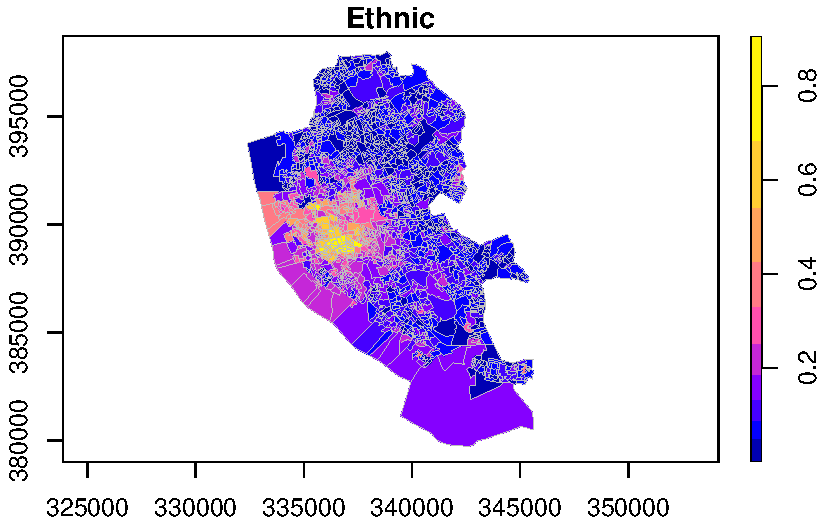
\includegraphics{03-data-wrangling_files/figure-pdf/unnamed-chunk-41-1.pdf}

To visualise a column in the spatial data frame, we can run:

\begin{Shaded}
\begin{Highlighting}[]
\CommentTok{\# map attributes, adding intervals}
\FunctionTok{plot}\NormalTok{(oa\_shp[}\StringTok{"Ethnic"}\NormalTok{], }\CommentTok{\# variable to visualise}
     \AttributeTok{key.pos =} \DecValTok{4}\NormalTok{, }
     \AttributeTok{axes =} \ConstantTok{TRUE}\NormalTok{, }
     \AttributeTok{key.width =} \FunctionTok{lcm}\NormalTok{(}\FloatTok{1.3}\NormalTok{), }
     \AttributeTok{key.length =} \FloatTok{1.}\NormalTok{,}
     \AttributeTok{breaks =} \StringTok{"jenks"}\NormalTok{, }\CommentTok{\# algorithm to categorise the data}
     \AttributeTok{lwd =} \FloatTok{0.1}\NormalTok{, }
     \AttributeTok{border =} \StringTok{\textquotesingle{}grey\textquotesingle{}}\NormalTok{) }\CommentTok{\# boundary colour}
\end{Highlighting}
\end{Shaded}

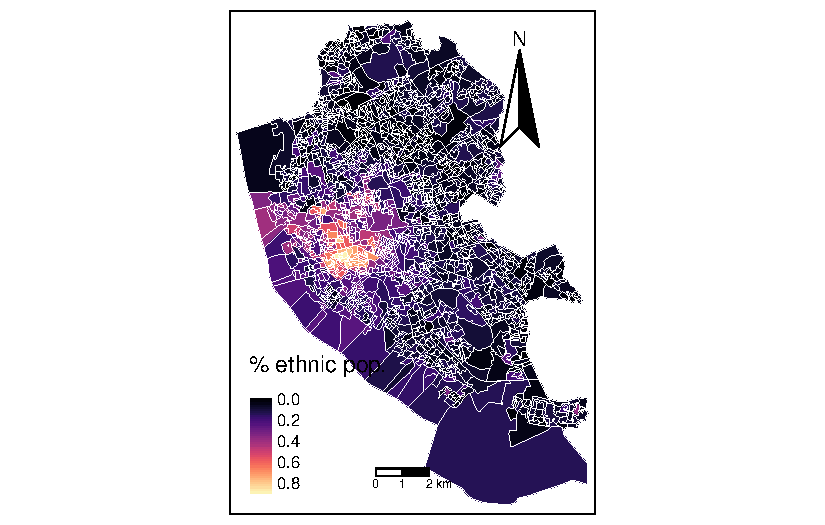
\includegraphics{03-data-wrangling_files/figure-pdf/unnamed-chunk-42-1.pdf}

\marginnote{\begin{footnotesize}

\begin{tcolorbox}[enhanced jigsaw, colframe=quarto-callout-tip-color-frame, leftrule=.75mm, arc=.35mm, breakable, opacityback=0, bottomrule=.15mm, colback=white, rightrule=.15mm, toprule=.15mm, left=2mm]

\textbf{Task}

What is the key pattern emerging from this map?

\end{tcolorbox}

\end{footnotesize}}

Let us now explore \texttt{ggplot} or \texttt{tmap}.

\textbf{Using \texttt{ggplot}}

We can visualise spatial data frames using \texttt{ggplot} fairly
easily. \texttt{ggplot} is a generic sets of functions which was not
specifically designed for spatial mapping, but it is fairly flexible
that allows producing great spatial data visualisations.

Following the grammar of \texttt{ggplot}, we plot spatial data drawing
layers. \texttt{ggplot} has a basic structure of three components:

\begin{itemize}
\tightlist
\item
  The data i.e.~\texttt{ggplot(\ data\ =\ *data\ frame*)}.
\item
  Geometries i.e.~\texttt{geom\_xxx(\ )}.
\item
  Aesthetic mapping i.e.~\texttt{aes(x=*variable*,\ y=*variable*)}
\end{itemize}

We can put these three components together using \texttt{+}. This is
similar to the ways we apply the pipe operator in for tidyverse. The
latter component of aesthetic mapping can be added in both the
\texttt{ggplot} and \texttt{geom\_xxx} functions.

To map our data, we can then run:

\begin{Shaded}
\begin{Highlighting}[]
\FunctionTok{ggplot}\NormalTok{(}\AttributeTok{data =}\NormalTok{ oa\_shp, }\FunctionTok{aes}\NormalTok{( }\AttributeTok{fill =}\NormalTok{ Ethnic) ) }\SpecialCharTok{+} \CommentTok{\# add data frame and variable to map}
  \FunctionTok{geom\_sf}\NormalTok{(}\AttributeTok{colour =} \StringTok{"gray60"}\NormalTok{,  }\CommentTok{\# colour line}
          \AttributeTok{size =} \FloatTok{0.1}\NormalTok{) }\CommentTok{\# line size}
\end{Highlighting}
\end{Shaded}

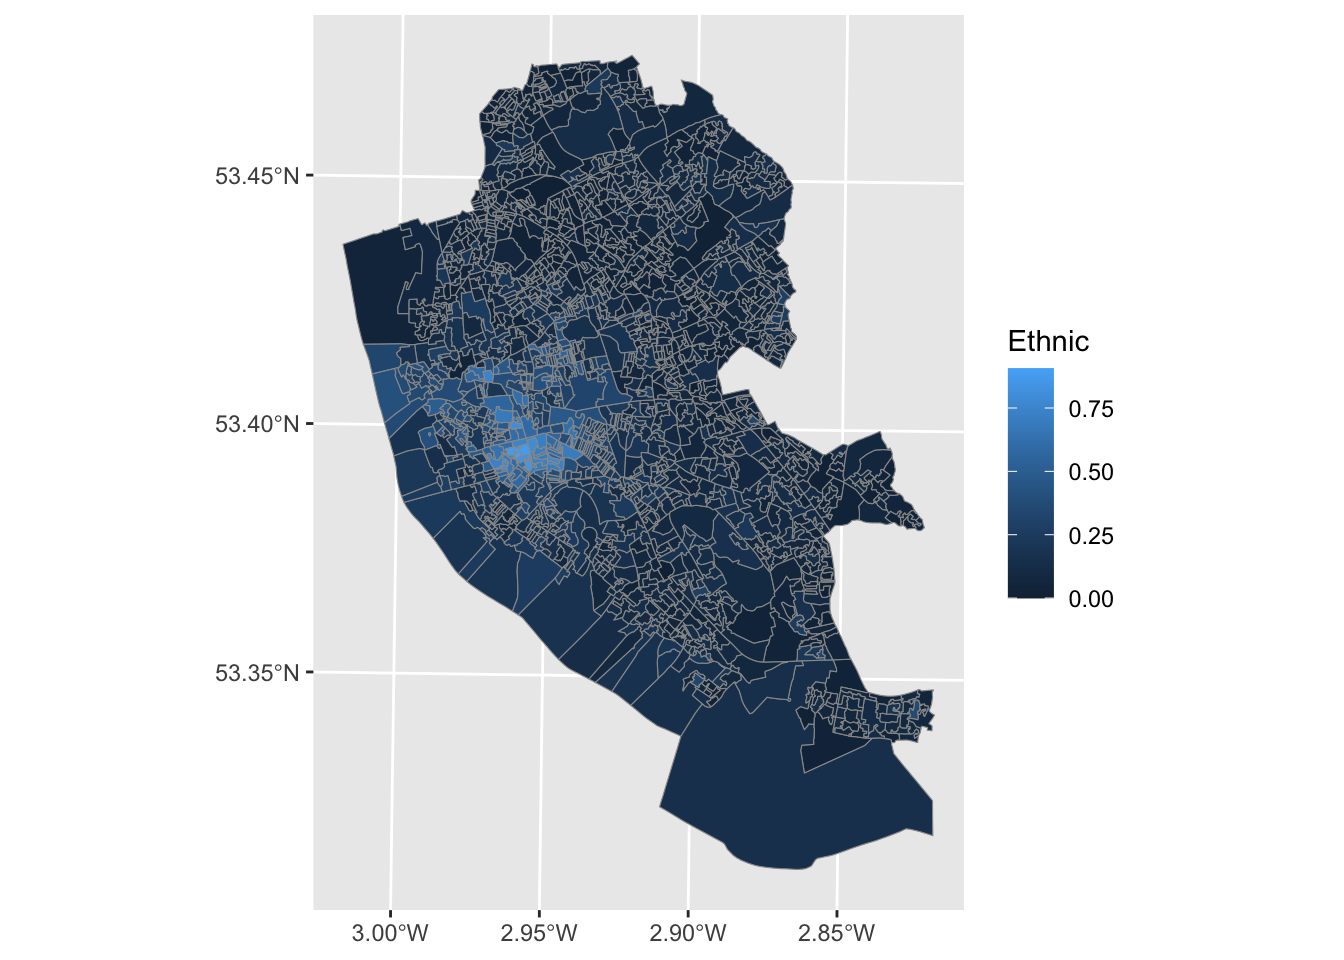
\includegraphics{03-data-wrangling_files/figure-pdf/unnamed-chunk-43-1.pdf}

We can change the colour palette by using a different colour palette. We
can use the
\href{https://cran.r-project.org/web/packages/viridis/vignettes/intro-to-viridis.html}{viridis}
package. The power of \texttt{viridis} is that it uses color scales that
visually pleasing, colorblind friendly, print well in gray scale, and
can be used for both categorical and continuous data. For categorical
data you can also use
\href{https://colorbrewer2.org/\#type=sequential&scheme=BuGn&n=3}{ColourBrewer}.

So let us (1) change the colour pallete to viridis, (2) remove the
colour of the boundaries, and (3) replace the theme with the theme we
will be using for the book. Let's read the theme first and then
implement these changes.

The \texttt{ggplot} themes for the book are in a file called
\texttt{data-visualisation\_theme.R} in the \texttt{style} folder. We
read this file by running:

\begin{Shaded}
\begin{Highlighting}[]
\FunctionTok{source}\NormalTok{(}\StringTok{"./style/data{-}visualisation\_theme.R"}\NormalTok{)}
\end{Highlighting}
\end{Shaded}

\begin{verbatim}
Loading required package: sysfonts
\end{verbatim}

\begin{verbatim}
Loading required package: showtextdb
\end{verbatim}

We can now implement our changes:

\begin{Shaded}
\begin{Highlighting}[]
\FunctionTok{ggplot}\NormalTok{(}\AttributeTok{data =}\NormalTok{ oa\_shp, }\FunctionTok{aes}\NormalTok{( }\AttributeTok{fill =}\NormalTok{ Ethnic) ) }\SpecialCharTok{+} \CommentTok{\# add data frame and variable to map}
  \FunctionTok{geom\_sf}\NormalTok{(}\AttributeTok{colour =} \StringTok{"transparent"}\NormalTok{) }\SpecialCharTok{+} \CommentTok{\# colour line}
  \FunctionTok{scale\_fill\_viridis}\NormalTok{( }\AttributeTok{option =} \StringTok{"viridis"}\NormalTok{ ) }\SpecialCharTok{+} \CommentTok{\# add viridis colour scheme}
  \FunctionTok{theme\_map\_tufte}\NormalTok{()}
\end{Highlighting}
\end{Shaded}

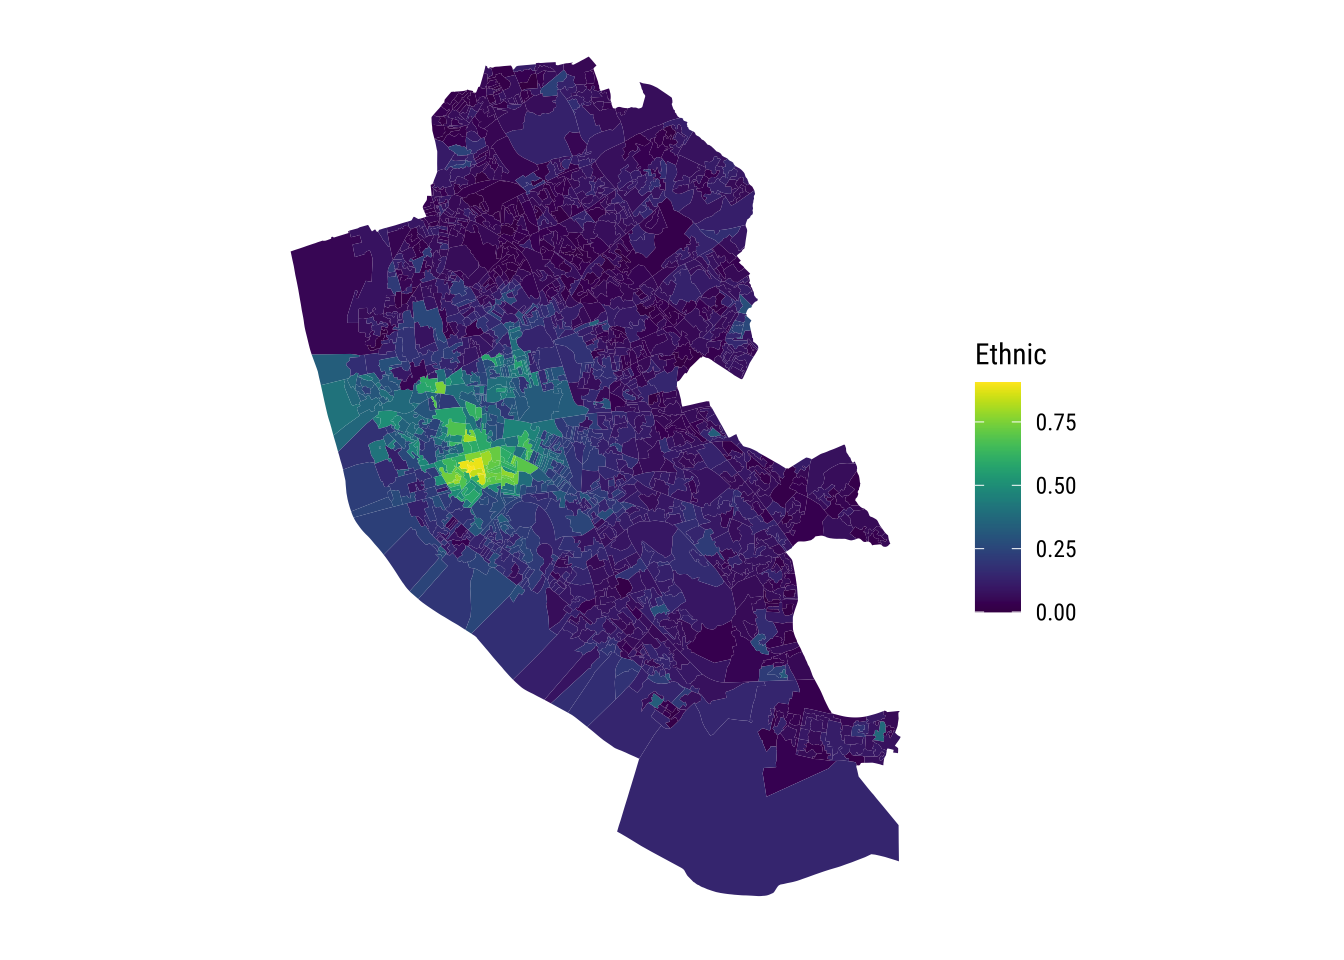
\includegraphics{03-data-wrangling_files/figure-pdf/unnamed-chunk-45-1.pdf}

To master \texttt{ggplot}, see Wickham (2009).

\textbf{Using \texttt{tmap}}

Similar to \texttt{ggplot2}, \texttt{tmap} is based on the idea of a
`grammar of graphics' which involves a separation between the input data
and aesthetics (i.e.~the way data are visualised). Each data set can be
mapped in various different ways, including location as defined by its
geometry, colour and other features. The basic building block is
\texttt{tm\_shape()} (which defines input data), followed by one or more
layer elements such as \texttt{tm\_fill()} and \texttt{tm\_dots()}.

\begin{Shaded}
\begin{Highlighting}[]
\CommentTok{\# ensure geometry is valid}
\NormalTok{oa\_shp }\OtherTok{=}\NormalTok{ sf}\SpecialCharTok{::}\FunctionTok{st\_make\_valid}\NormalTok{(oa\_shp)}

\CommentTok{\# map}
\NormalTok{legend\_title }\OtherTok{=} \FunctionTok{expression}\NormalTok{(}\StringTok{"\% ethnic pop."}\NormalTok{)}
\NormalTok{map\_oa }\OtherTok{=} \FunctionTok{tm\_shape}\NormalTok{(oa\_shp) }\SpecialCharTok{+}
  \FunctionTok{tm\_fill}\NormalTok{(}\AttributeTok{col =} \StringTok{"Ethnic"}\NormalTok{, }\AttributeTok{title =}\NormalTok{ legend\_title, }\AttributeTok{palette =} \FunctionTok{magma}\NormalTok{(}\DecValTok{256}\NormalTok{), }\AttributeTok{style =} \StringTok{"cont"}\NormalTok{) }\SpecialCharTok{+} \CommentTok{\# add fill}
  \FunctionTok{tm\_borders}\NormalTok{(}\AttributeTok{col =} \StringTok{"white"}\NormalTok{, }\AttributeTok{lwd =}\NormalTok{ .}\DecValTok{01}\NormalTok{)  }\SpecialCharTok{+} \CommentTok{\# add borders}
  \FunctionTok{tm\_compass}\NormalTok{(}\AttributeTok{type =} \StringTok{"arrow"}\NormalTok{, }\AttributeTok{position =} \FunctionTok{c}\NormalTok{(}\StringTok{"right"}\NormalTok{, }\StringTok{"top"}\NormalTok{) , }\AttributeTok{size =} \DecValTok{4}\NormalTok{) }\SpecialCharTok{+} \CommentTok{\# add compass}
  \FunctionTok{tm\_scale\_bar}\NormalTok{(}\AttributeTok{breaks =} \FunctionTok{c}\NormalTok{(}\DecValTok{0}\NormalTok{,}\DecValTok{1}\NormalTok{,}\DecValTok{2}\NormalTok{), }\AttributeTok{text.size =} \FloatTok{0.5}\NormalTok{, }\AttributeTok{position =}  \FunctionTok{c}\NormalTok{(}\StringTok{"center"}\NormalTok{, }\StringTok{"bottom"}\NormalTok{)) }\CommentTok{\# add scale bar}
\NormalTok{map\_oa}
\end{Highlighting}
\end{Shaded}

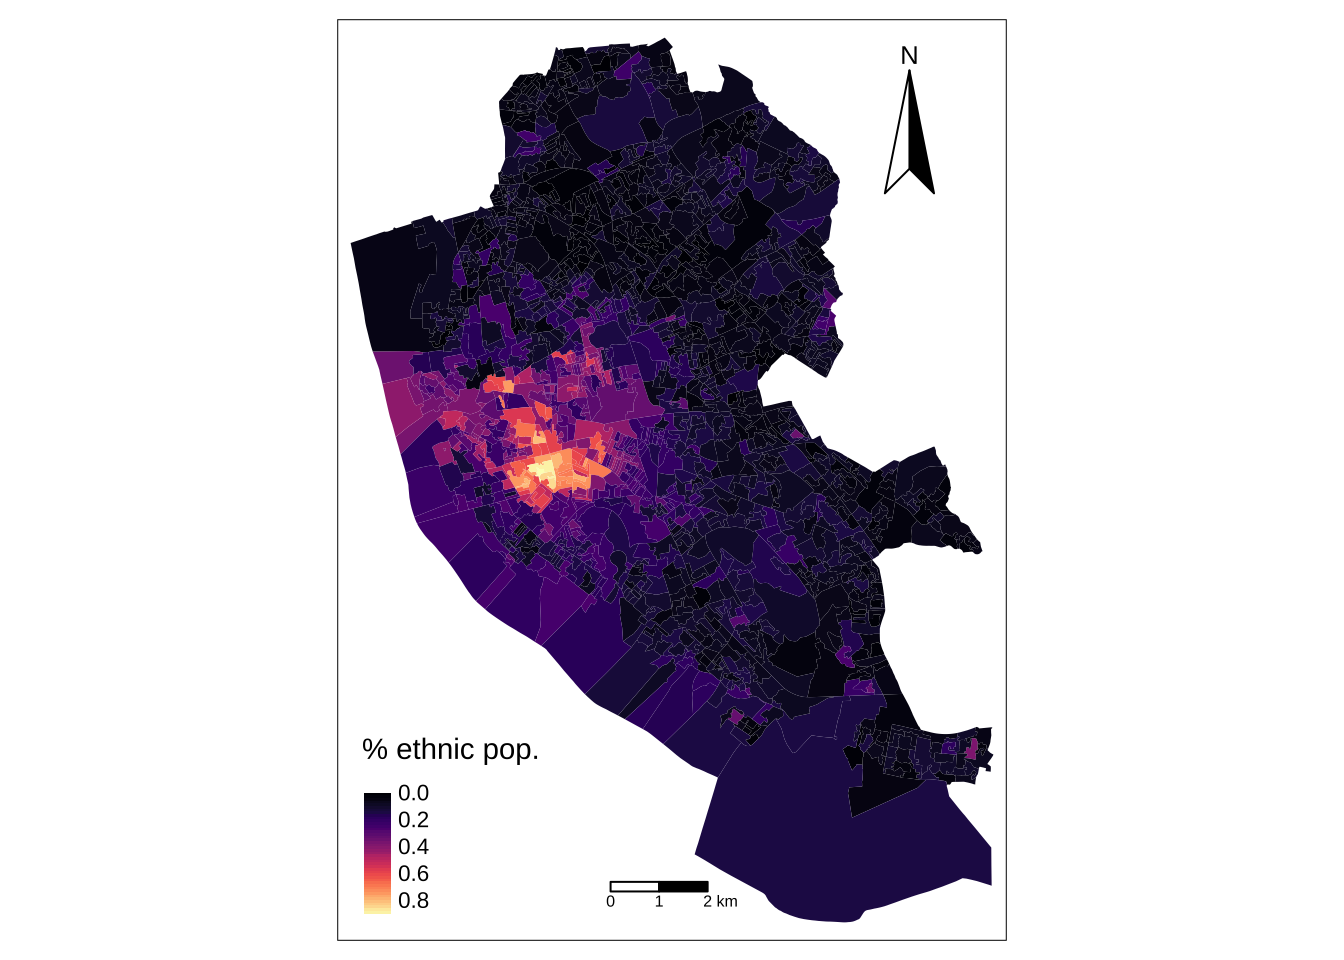
\includegraphics{03-data-wrangling_files/figure-pdf/unnamed-chunk-46-1.pdf}

Note that the operation \texttt{+}, as for \texttt{ggplot} is used to
add new layers. You can set style themes by \texttt{tm\_style}. To
visualise the existing styles use \texttt{tmap\_style\_catalogue()}. An
advantage of \texttt{tmap} is that you can easily create an interactive
map by running \texttt{tmap\_mode}.

\begin{Shaded}
\begin{Highlighting}[]
\FunctionTok{tmap\_mode}\NormalTok{(}\StringTok{"view"}\NormalTok{)}
\end{Highlighting}
\end{Shaded}

\begin{verbatim}
tmap mode set to interactive viewing
\end{verbatim}

\begin{Shaded}
\begin{Highlighting}[]
\NormalTok{map\_oa}
\end{Highlighting}
\end{Shaded}

\begin{verbatim}
Compass not supported in view mode.
\end{verbatim}

\begin{verbatim}
Warning: In view mode, scale bar breaks are ignored.
\end{verbatim}

\includegraphics{03-data-wrangling_files/figure-pdf/unnamed-chunk-47-1.pdf}

\marginnote{\begin{footnotesize}

\begin{tcolorbox}[enhanced jigsaw, colframe=quarto-callout-tip-color-frame, leftrule=.75mm, arc=.35mm, breakable, opacityback=0, bottomrule=.15mm, colback=white, rightrule=.15mm, toprule=.15mm, left=2mm]

\textbf{Task}

Try mapping other variables in the spatial data frame. Where do
population aged 60 and over concentrate?

\end{tcolorbox}

\end{footnotesize}}

\subsection{Comparing geographies}\label{comparing-geographies}

If you recall, one of the key issues of working with spatial data is the
modifiable area unit problem (MAUP) - see (\textbf{spatial\_data?}). To
get a sense of the effects of MAUP, we analyse differences in the
spatial patterns of the ethnic population in Liverpool between Middle
Layer Super Output Areas (MSOAs) and OAs. So we map these geographies
together.

\marginnote{\begin{footnotesize}

\begin{tcolorbox}[enhanced jigsaw, title=\textcolor{quarto-callout-note-color}{\faInfo}\hspace{0.5em}{Note}, opacitybacktitle=0.6, arc=.35mm, coltitle=black, colback=white, colbacktitle=quarto-callout-note-color!10!white, toptitle=1mm, colframe=quarto-callout-note-color-frame, leftrule=.75mm, breakable, opacityback=0, bottomrule=.15mm, left=2mm, titlerule=0mm, rightrule=.15mm, toprule=.15mm, bottomtitle=1mm]

The first line of the chunk code include \texttt{tmap\_mode("plot")}
which tells R that we want a static map. \texttt{tmap\_mode} works like
a switch to interactive and non-interactive mapping.

\end{tcolorbox}

\end{footnotesize}}

\begin{Shaded}
\begin{Highlighting}[]
\FunctionTok{tmap\_mode}\NormalTok{(}\StringTok{"plot"}\NormalTok{)}
\end{Highlighting}
\end{Shaded}

\begin{verbatim}
tmap mode set to plotting
\end{verbatim}

\begin{Shaded}
\begin{Highlighting}[]
\CommentTok{\# read data at the msoa level}
\NormalTok{msoa\_shp }\OtherTok{\textless{}{-}} \FunctionTok{st\_read}\NormalTok{(}\StringTok{"data/census/Liverpool\_MSOA.shp"}\NormalTok{)}
\end{Highlighting}
\end{Shaded}

\begin{verbatim}
Reading layer `Liverpool_MSOA' from data source 
  `/Users/franciscorowe/Dropbox/Francisco/uol/teaching/envs453/202324/san/data/census/Liverpool_MSOA.shp' 
  using driver `ESRI Shapefile'
Simple feature collection with 61 features and 16 fields
Geometry type: MULTIPOLYGON
Dimension:     XY
Bounding box:  xmin: 333086.1 ymin: 381426.3 xmax: 345636 ymax: 397980.1
Projected CRS: Transverse_Mercator
\end{verbatim}

\begin{Shaded}
\begin{Highlighting}[]
\CommentTok{\# ensure geometry is valid}
\NormalTok{msoa\_shp }\OtherTok{=}\NormalTok{ sf}\SpecialCharTok{::}\FunctionTok{st\_make\_valid}\NormalTok{(msoa\_shp)}

\CommentTok{\# create a map}
\NormalTok{map\_msoa }\OtherTok{=} \FunctionTok{tm\_shape}\NormalTok{(msoa\_shp) }\SpecialCharTok{+}
  \FunctionTok{tm\_fill}\NormalTok{(}\AttributeTok{col =} \StringTok{"Ethnic"}\NormalTok{, }\AttributeTok{title =}\NormalTok{ legend\_title, }\AttributeTok{palette =} \FunctionTok{magma}\NormalTok{(}\DecValTok{256}\NormalTok{), }\AttributeTok{style =} \StringTok{"cont"}\NormalTok{) }\SpecialCharTok{+} 
  \FunctionTok{tm\_borders}\NormalTok{(}\AttributeTok{col =} \StringTok{"white"}\NormalTok{, }\AttributeTok{lwd =}\NormalTok{ .}\DecValTok{01}\NormalTok{)  }\SpecialCharTok{+} 
  \FunctionTok{tm\_compass}\NormalTok{(}\AttributeTok{type =} \StringTok{"arrow"}\NormalTok{, }\AttributeTok{position =} \FunctionTok{c}\NormalTok{(}\StringTok{"right"}\NormalTok{, }\StringTok{"top"}\NormalTok{) , }\AttributeTok{size =} \DecValTok{4}\NormalTok{) }\SpecialCharTok{+} 
  \FunctionTok{tm\_scale\_bar}\NormalTok{(}\AttributeTok{breaks =} \FunctionTok{c}\NormalTok{(}\DecValTok{0}\NormalTok{,}\DecValTok{1}\NormalTok{,}\DecValTok{2}\NormalTok{), }\AttributeTok{text.size =} \FloatTok{0.5}\NormalTok{, }\AttributeTok{position =}  \FunctionTok{c}\NormalTok{(}\StringTok{"center"}\NormalTok{, }\StringTok{"bottom"}\NormalTok{)) }

\CommentTok{\# arrange maps }
\FunctionTok{tmap\_arrange}\NormalTok{(map\_msoa, map\_oa) }
\end{Highlighting}
\end{Shaded}

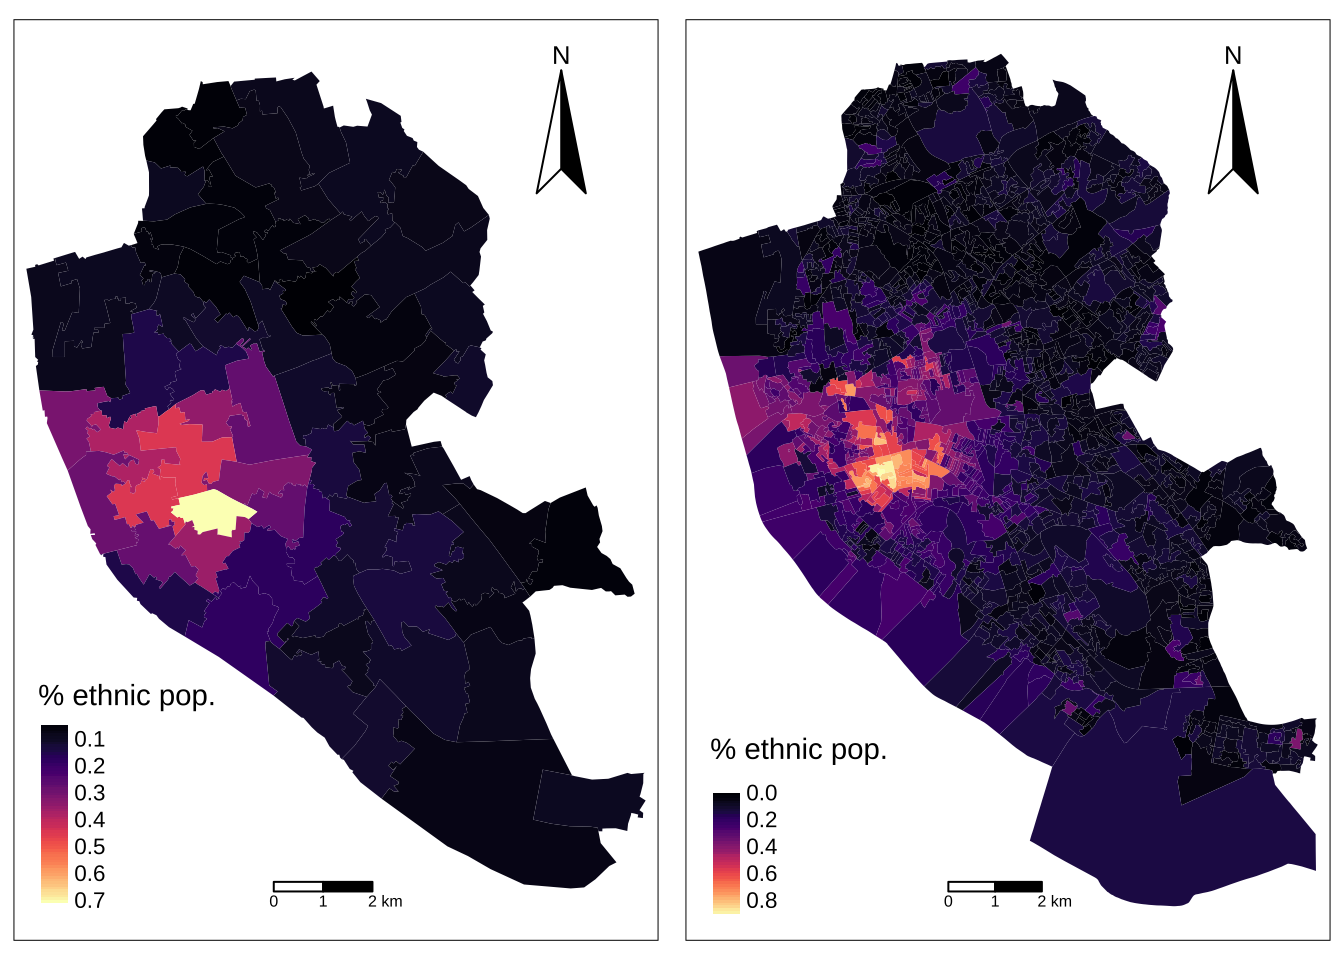
\includegraphics{03-data-wrangling_files/figure-pdf/unnamed-chunk-48-1.pdf}

\marginnote{\begin{footnotesize}

\begin{tcolorbox}[enhanced jigsaw, colframe=quarto-callout-tip-color-frame, leftrule=.75mm, arc=.35mm, breakable, opacityback=0, bottomrule=.15mm, colback=white, rightrule=.15mm, toprule=.15mm, left=2mm]

\textbf{Task}

What differences do you see between OAs and MSOAs?

Can you identify areas of spatial clustering? Where are they?

\end{tcolorbox}

\end{footnotesize}}

\bookmarksetup{startatroot}

\chapter{Point Data Analysis}\label{sec-chp4}

This chapter is based on the following references, which are great
follow-up's on the topic:

\begin{itemize}
\tightlist
\item
  Lovelace, Nowosad, and Muenchow (2019) offer a great introduction.
\item
  Chapter 6 of Brunsdon and Comber (2015), in particular subsections 6.3
  and 6.7.
\item
  R. S. Bivand, Pebesma, and Gómez-Rubio (2013) provides an in-depth
  treatment of spatial data in R.
\end{itemize}

\section{Dependencies}\label{dependencies-1}

We will rely on the following libraries in this section, all of them
included in Section~\ref{sec-dependencies}:

\begin{Shaded}
\begin{Highlighting}[]
\CommentTok{\# data manipulation, transformation and visualisation}
\FunctionTok{library}\NormalTok{(tidyverse)}
\CommentTok{\# spatial data manipulation}
\FunctionTok{library}\NormalTok{(sf)}
\FunctionTok{library}\NormalTok{(sp)}
\CommentTok{\# data visualisation}
\FunctionTok{library}\NormalTok{(gridExtra)}
\CommentTok{\# basemap}
\FunctionTok{library}\NormalTok{(basemapR)}
\CommentTok{\# interpolation}
\FunctionTok{library}\NormalTok{(gstat)}
\FunctionTok{library}\NormalTok{(hexbin)}
\end{Highlighting}
\end{Shaded}

Before we start any analysis, let us set the path to the directory where
we are working. We can easily do that with \texttt{setwd()}. Please
replace in the following line the path to the folder where you have
placed this file -and where the \texttt{house\_transactions} folder with
the data lives.

\section{Data}\label{data}

For this session, we will use the set of Airbnb properties for San Diego
(US), borrowed from the ``Geographic Data Science with Python'' book
(see
\href{https://geographicdata.science/book/data/airbnb/regression_cleaning.html}{here}
for more info on the dataset source). This covers the point location of
properties advertised on the Airbnb website in the San Diego region.

Let us start by reading the data, which comes in a GeoJSON:

\begin{Shaded}
\begin{Highlighting}[]
\NormalTok{db }\OtherTok{\textless{}{-}} \FunctionTok{st\_read}\NormalTok{(}\StringTok{"data/abb\_sd/regression\_db.geojson"}\NormalTok{)}
\end{Highlighting}
\end{Shaded}

\begin{verbatim}
Reading layer `regression_db' from data source 
  `/Users/franciscorowe/Dropbox/Francisco/uol/teaching/envs453/202324/san/data/abb_sd/regression_db.geojson' 
  using driver `GeoJSON'
Simple feature collection with 6110 features and 19 fields
Geometry type: POINT
Dimension:     XY
Bounding box:  xmin: -117.2812 ymin: 32.57349 xmax: -116.9553 ymax: 33.08311
Geodetic CRS:  WGS 84
\end{verbatim}

We can then examine the columns of the table with the \texttt{colnames}
method:

\begin{Shaded}
\begin{Highlighting}[]
\FunctionTok{colnames}\NormalTok{(db)}
\end{Highlighting}
\end{Shaded}

\begin{verbatim}
 [1] "accommodates"       "bathrooms"          "bedrooms"          
 [4] "beds"               "neighborhood"       "pool"              
 [7] "d2balboa"           "coastal"            "price"             
[10] "log_price"          "id"                 "pg_Apartment"      
[13] "pg_Condominium"     "pg_House"           "pg_Other"          
[16] "pg_Townhouse"       "rt_Entire_home.apt" "rt_Private_room"   
[19] "rt_Shared_room"     "geometry"          
\end{verbatim}

The rest of this session will focus on two main elements of the table:
the spatial dimension (as stored in the point coordinates), and the
nightly price values, expressed in USD and contained in the
\texttt{price} column. To get a sense of what they look like first, let
us plot both. We can get a quick look at the non-spatial distribution of
house values with the following commands:

\begin{Shaded}
\begin{Highlighting}[]
\CommentTok{\# Create the histogram}
\FunctionTok{qplot}\NormalTok{( }\AttributeTok{data =}\NormalTok{ db, }\AttributeTok{x =}\NormalTok{ price)}
\end{Highlighting}
\end{Shaded}

\begin{verbatim}
Warning: `qplot()` was deprecated in ggplot2 3.4.0.
\end{verbatim}

\begin{verbatim}
`stat_bin()` using `bins = 30`. Pick better value with `binwidth`.
\end{verbatim}

\begin{figure}[H]

{\centering \includegraphics{04-points_files/figure-pdf/unnamed-chunk-5-1.pdf}

}

\caption{Raw AirBnb prices in San Diego}

\end{figure}%

This basically shows there is a lot of values concentrated around the
lower end of the distribution but a few very large ones. A usual
transformation to \emph{shrink} these differences is to take logarithms.
The original table already contains an additional column with the
logarithm of each price (\texttt{log\_price}).

\begin{Shaded}
\begin{Highlighting}[]
\CommentTok{\# Create the histogram}
\FunctionTok{qplot}\NormalTok{( }\AttributeTok{data =}\NormalTok{ db, }\AttributeTok{x =}\NormalTok{ log\_price )}
\end{Highlighting}
\end{Shaded}

\begin{verbatim}
`stat_bin()` using `bins = 30`. Pick better value with `binwidth`.
\end{verbatim}

\includegraphics{04-points_files/figure-pdf/unnamed-chunk-6-1.pdf}

To obtain the spatial distribution of these houses, we need to focus on
the \texttt{geometry} column. The easiest, quickest (and also
``dirtiest'') way to get a sense of what the data look like over space
is using \texttt{plot}:

\begin{Shaded}
\begin{Highlighting}[]
\FunctionTok{plot}\NormalTok{(}\FunctionTok{st\_geometry}\NormalTok{(db))}
\end{Highlighting}
\end{Shaded}

\includegraphics{04-points_files/figure-pdf/unnamed-chunk-7-1.pdf}

Now this has the classic problem of cluttering: some portions of the map
have so many points that we can't tell what the distribution is like. To
get around this issue, there are two solutions: binning and smoothing.

\section{Binning}\label{binning}

The two-dimensional sister of histograms are binning maps: we divide
each of the two dimensions into ``buckets'', and count how many points
fall within each bucket. Unlike histograms, we encode that count with a
color gradient rather than a bar chart over an additional dimension (for
that, we would need a 3D plot). These ``buckets'' can be squares (left)
or hexagons (right):

\begin{Shaded}
\begin{Highlighting}[]
      \CommentTok{\# Squared binning}
\CommentTok{\# Set up plot}
\NormalTok{sqbin }\OtherTok{\textless{}{-}} \FunctionTok{ggplot}\NormalTok{( ) }\SpecialCharTok{+} 
\CommentTok{\# Add 2D binning with the XY coordinates as}
\CommentTok{\# a dataframe}
  \FunctionTok{geom\_bin2d}\NormalTok{(}
    \AttributeTok{data =} \FunctionTok{as.data.frame}\NormalTok{( }\FunctionTok{st\_coordinates}\NormalTok{( db ) ), }
    \FunctionTok{aes}\NormalTok{( }\AttributeTok{x =}\NormalTok{ X, }\AttributeTok{y =}\NormalTok{ Y)}
\NormalTok{  ) }\SpecialCharTok{+} 
  \CommentTok{\# set theme }
  \FunctionTok{theme\_plot\_tufte}\NormalTok{()}
      \CommentTok{\# Hex binning}
\CommentTok{\# Set up plot}
\NormalTok{hexbin }\OtherTok{\textless{}{-}} \FunctionTok{ggplot}\NormalTok{() }\SpecialCharTok{+}
\CommentTok{\# Add hex binning with the XY coordinates as}
\CommentTok{\# a dataframe }
  \FunctionTok{geom\_hex}\NormalTok{(}
    \AttributeTok{data =} \FunctionTok{as.data.frame}\NormalTok{( }\FunctionTok{st\_coordinates}\NormalTok{( db ) ),}
    \FunctionTok{aes}\NormalTok{( }\AttributeTok{x =}\NormalTok{ X, }\AttributeTok{y =}\NormalTok{ Y)}
\NormalTok{  ) }\SpecialCharTok{+}
\CommentTok{\# Use viridis for color encoding (recommended)}
  \FunctionTok{scale\_fill\_continuous}\NormalTok{( }\AttributeTok{type =} \StringTok{"viridis"}\NormalTok{ ) }\SpecialCharTok{+}
  \FunctionTok{theme\_plot\_tufte}\NormalTok{()}
      \CommentTok{\# Bind in subplots}
\FunctionTok{grid.arrange}\NormalTok{( sqbin, hexbin, }\AttributeTok{ncol =} \DecValTok{2}\NormalTok{ ) }
\end{Highlighting}
\end{Shaded}

\includegraphics{04-points_files/figure-pdf/unnamed-chunk-8-1.pdf}

\section{KDE}\label{kde}

Kernel Density Estimation (KDE) is a technique that creates a
\emph{continuous} representation of the distribution of a given
variable, such as house prices. Although theoretically it can be applied
to any dimension, usually, KDE is applied to either one or two
dimensions.

\subsection{One-dimensional KDE}\label{one-dimensional-kde}

KDE over a single dimension is essentially a contiguous version of a
histogram. We can see that by overlaying a KDE on top of the histogram
of logs that we have created before:

\begin{Shaded}
\begin{Highlighting}[]
\CommentTok{\# Create the base}
\NormalTok{base }\OtherTok{\textless{}{-}} \FunctionTok{ggplot}\NormalTok{(db, }\FunctionTok{aes}\NormalTok{(}\AttributeTok{x=}\NormalTok{log\_price))}
\CommentTok{\# Histogram}
\NormalTok{hist }\OtherTok{\textless{}{-}}\NormalTok{ base }\SpecialCharTok{+} 
  \FunctionTok{geom\_histogram}\NormalTok{(}\AttributeTok{bins=}\DecValTok{50}\NormalTok{, }\FunctionTok{aes}\NormalTok{(}\AttributeTok{y=}\NormalTok{..density..))}
\CommentTok{\# Overlay density plot}
\NormalTok{kde }\OtherTok{\textless{}{-}}\NormalTok{ hist }\SpecialCharTok{+} 
  \FunctionTok{geom\_density}\NormalTok{(}\AttributeTok{fill=}\StringTok{"\#FF6666"}\NormalTok{, }\AttributeTok{alpha=}\FloatTok{0.5}\NormalTok{, }\AttributeTok{colour=}\StringTok{"\#FF6666"}\NormalTok{) }\SpecialCharTok{+}
  \FunctionTok{theme\_plot\_tufte}\NormalTok{()}
\NormalTok{kde}
\end{Highlighting}
\end{Shaded}

\begin{verbatim}
Warning: The dot-dot notation (`..density..`) was deprecated in ggplot2 3.4.0.
i Please use `after_stat(density)` instead.
\end{verbatim}

\includegraphics{04-points_files/figure-pdf/unnamed-chunk-9-1.pdf}

The key idea is that we are smoothing out the discrete binning that the
histogram involves. Note how the histogram is exactly the same as above
shape-wise, but it has been rescalend on the Y axis to reflect
probabilities rather than counts.

\subsection{Two-dimensional (spatial)
KDE}\label{two-dimensional-spatial-kde}

Geography, at the end of the day, is usually represented as a
two-dimensional space where we locate objects using a system of dual
coordinates, \texttt{X} and \texttt{Y} (or latitude and longitude).
Thanks to that, we can use the same technique as above to obtain a
smooth representation of the distribution of a two-dimensional variable.
The crucial difference is that, instead of obtaining a curve as the
output, we will create a \emph{surface}, where intensity will be
represented with a color gradient, rather than with the second
dimension, as it is the case in the figure above.

To create a spatial KDE in R, we can use general tooling for non-spatial
points, such as the \texttt{stat\_density2d\_filled} method:

\begin{Shaded}
\begin{Highlighting}[]
\CommentTok{\# Create the KDE surface}
\NormalTok{kde }\OtherTok{\textless{}{-}} \FunctionTok{ggplot}\NormalTok{(}\AttributeTok{data =}\NormalTok{ db) }\SpecialCharTok{+}
  \FunctionTok{stat\_density2d\_filled}\NormalTok{(}\AttributeTok{alpha =} \DecValTok{1}\NormalTok{,}
    \AttributeTok{data =} \FunctionTok{as.data.frame}\NormalTok{(}\FunctionTok{st\_coordinates}\NormalTok{(db)), }
    \FunctionTok{aes}\NormalTok{(}\AttributeTok{x =}\NormalTok{ X, }\AttributeTok{y =}\NormalTok{ Y),}
    \AttributeTok{n =} \DecValTok{100}
\NormalTok{  ) }\SpecialCharTok{+}
  \CommentTok{\# Tweak the color gradient}
  \FunctionTok{scale\_color\_viridis\_c}\NormalTok{() }\SpecialCharTok{+}
  \CommentTok{\# White theme}
  \FunctionTok{theme\_plot\_tufte}\NormalTok{() }
\NormalTok{kde}
\end{Highlighting}
\end{Shaded}

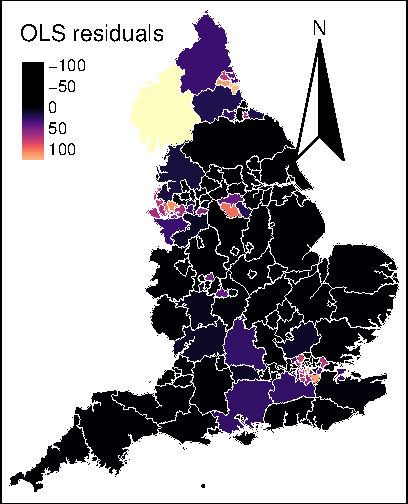
\includegraphics{04-points_files/figure-pdf/unnamed-chunk-10-1.pdf}

This approach generates a surface that represents the density of dots,
that is an estimation of the probability of finding a house transaction
at a given coordinate. However, without any further information, they
are hard to interpret and link with previous knowledge of the area. To
bring such context to the figure, we can plot an underlying basemap,
using a cloud provider such as Google Maps or, as in this case,
OpenStreetMap. To do it, we will leverage the library \texttt{basemapR},
which is designed to play nicely with the \texttt{ggplot2} family (hence
the seemingly counterintuitive example above). Before we can plot them
with the online map, we need to reproject them though.

\begin{Shaded}
\begin{Highlighting}[]
\NormalTok{bbox\_db }\OtherTok{\textless{}{-}} \FunctionTok{st\_bbox}\NormalTok{(db)}
\FunctionTok{ggplot}\NormalTok{() }\SpecialCharTok{+}
  \FunctionTok{base\_map}\NormalTok{(bbox\_db, }\AttributeTok{increase\_zoom =} \DecValTok{2}\NormalTok{, }\AttributeTok{basemap =} \StringTok{"positron"}\NormalTok{) }\SpecialCharTok{+}
  \CommentTok{\#geom\_sf(data = db, fill = NA) +}
  \FunctionTok{stat\_density2d\_filled}\NormalTok{(}\AttributeTok{alpha =} \FloatTok{0.7}\NormalTok{,}
    \AttributeTok{data =} \FunctionTok{as.data.frame}\NormalTok{(}\FunctionTok{st\_coordinates}\NormalTok{(db)), }
    \FunctionTok{aes}\NormalTok{(}\AttributeTok{x =}\NormalTok{ X, }\AttributeTok{y =}\NormalTok{ Y),}
    \AttributeTok{n =} \DecValTok{100}
\NormalTok{  )}
\end{Highlighting}
\end{Shaded}

\includegraphics{04-points_files/figure-pdf/unnamed-chunk-11-1.pdf}

\section{Spatial Interpolation}\label{spatial-interpolation}

The previous section demonstrates how to visualize the distribution of a
set of spatial objects represented as points. In particular, given a
bunch of house locations, it shows how one can effectively visualize
their distribution over space and get a sense of the density of
occurrences. Such visualization, because it is based on KDE, is based on
a smooth continuum, rather than on a discrete approach (as a choropleth
would do, for example).

Many times however, we are not particularly interested in learning about
the density of occurrences, but about the distribution of a given value
attached to each location. Think for example of weather stations and
temperature: the location of the stations is no secret and rarely
changes, so it is not of particular interest to visualize the density of
stations; what we are usually interested instead is to know how
temperature is distributed over space, given we only measure it in a few
places. One could argue the example we have been working with so far,
house prices in AirBnb, fits into this category as well: although where
a house is advertised may be of relevance, more often we are interested
in finding out what the ``surface of price'' looks like. Rather than
\emph{where are most houses being advertised?} we usually want to know
\emph{where the most expensive or most affordable} houses are located.

In cases where we are interested in creating a surface of a given value,
rather than a simple density surface of occurrences, KDE cannot help us.
In these cases, what we are interested in is \emph{spatial
interpolation}, a family of techniques that aim at exactly that:
creating continuous surfaces for a particular phenomenon
(e.g.~temperature, house prices) given only a finite sample of
observations. Spatial interpolation is a large field of research that is
still being actively developed and that can involve a substantial amount
of mathematical complexity in order to obtain the most accurate
estimates possible\footnote{There is also an important economic
  incentive to do this: some of the most popular applications are in the
  oil and gas or mining industries. In fact, the very creator of this
  technique, \href{https://en.wikipedia.org/wiki/Danie_G._Krige}{Danie
  G. Krige}, was a mining engineer. His name is usually used to nickname
  spatial interpolation as \emph{kriging}.}. In this chapter, we will
introduce the simplest possible way of interpolating values, hoping this
will give you a general understanding of the methodology and, if you are
interested, you can check out further literature. For example, Banerjee,
Carlin, and Gelfand (2014) or Cressie (2015) are hard but good
overviews.

\subsection{Inverse Distance Weight (IDW)
interpolation}\label{inverse-distance-weight-idw-interpolation}

The technique we will cover here is called \emph{Inverse Distance
Weighting}, or IDW for convenience. Brunsdon and Comber (2015) offer a
good description:

\begin{quote}
In the \emph{inverse distance weighting} (IDW) approach to
interpolation, to estimate the value of \(z\) at location \(x\) a
weighted mean of nearby observations is taken {[}\ldots{]}. To
accommodate the idea that observations of \(z\) at points closer to
\(x\) should be given more importance in the interpolation, greater
weight is given to these points {[}\ldots{]}

--- Page 204
\end{quote}

The math\footnote{Essentially, for any point \(x\) in space, the IDW
  estimate for value \(z\) is equivalent to
  \(\hat{z} (x) = \dfrac{\sum_i w_i z_i}{\sum_i w_i}\) where \(i\) are
  the observations for which we do have a value, and \(w_i\) is a weight
  given to location \(i\) based on its distance to \(x\).} is not
particularly complicated and may be found in detail elsewhere (the
reference above is a good starting point), so we will not spend too much
time on it. More relevant in this context is the intuition behind. The
idea is that we will create a surface of house price by smoothing many
values arranged along a regular grid and obtained by interpolating from
the known locations to the regular grid locations. This will give us
full and equal coverage to soundly perform the smoothing.

Enough chat, let's code\footnote{If you want a complementary view of
  point interpolation in R, you can read more on this
  \href{https://swilke-geoscience.net/post/2020-09-10-kriging_with_r/kriging/}{fantastic
  blog post}}.

From what we have just mentioned, there are a few steps to perform an
IDW spatial interpolation:

\begin{enumerate}
\def\labelenumi{\arabic{enumi}.}
\tightlist
\item
  Create a regular grid over the area where we have house transactions.
\item
  Obtain IDW estimates for each point in the grid, based on the values
  of \(k\) nearest neighbors.
\item
  Plot a smoothed version of the grid, effectively representing the
  surface of house prices.
\end{enumerate}

Let us go in detail into each of them\footnote{For the relevant
  calculations, we will be using the \texttt{gstat} library.}. First,
let us set up a grid for the extent of the bounding box of our data (not
the use of pipe, \texttt{\%\textgreater{}\%}, operator to chain
functions):

\begin{Shaded}
\begin{Highlighting}[]
\NormalTok{sd.grid }\OtherTok{\textless{}{-}}\NormalTok{ db }\SpecialCharTok{\%\textgreater{}\%}
  \FunctionTok{st\_bbox}\NormalTok{() }\SpecialCharTok{\%\textgreater{}\%}
  \FunctionTok{st\_as\_sfc}\NormalTok{() }\SpecialCharTok{\%\textgreater{}\%}
  \FunctionTok{st\_make\_grid}\NormalTok{(}
    \AttributeTok{n =} \DecValTok{100}\NormalTok{,}
    \AttributeTok{what =} \StringTok{"centers"}
\NormalTok{  ) }\SpecialCharTok{\%\textgreater{}\%}
  \FunctionTok{st\_as\_sf}\NormalTok{() }\SpecialCharTok{\%\textgreater{}\%}
  \FunctionTok{cbind}\NormalTok{(., }\FunctionTok{st\_coordinates}\NormalTok{(.))}
\end{Highlighting}
\end{Shaded}

The object \texttt{sd.grid} is a regular grid with 10,000
(\(100 \times 100\)) equally spaced cells:

\begin{Shaded}
\begin{Highlighting}[]
\NormalTok{sd.grid}
\end{Highlighting}
\end{Shaded}

\begin{verbatim}
Simple feature collection with 10000 features and 2 fields
Geometry type: POINT
Dimension:     XY
Bounding box:  xmin: -117.2795 ymin: 32.57604 xmax: -116.9569 ymax: 33.08056
Geodetic CRS:  WGS 84
First 10 features:
           X        Y                          x
1  -117.2795 32.57604 POINT (-117.2795 32.57604)
2  -117.2763 32.57604 POINT (-117.2763 32.57604)
3  -117.2730 32.57604  POINT (-117.273 32.57604)
4  -117.2698 32.57604 POINT (-117.2698 32.57604)
5  -117.2665 32.57604 POINT (-117.2665 32.57604)
6  -117.2632 32.57604 POINT (-117.2632 32.57604)
7  -117.2600 32.57604   POINT (-117.26 32.57604)
8  -117.2567 32.57604 POINT (-117.2567 32.57604)
9  -117.2535 32.57604 POINT (-117.2535 32.57604)
10 -117.2502 32.57604 POINT (-117.2502 32.57604)
\end{verbatim}

Now, \texttt{sd.grid} only contain the location of points to which we
wish to interpolate. That is, we now have our ``target'' geography for
which we'd like to have AirBnb prices, but we don't have price
estimates. For that, on to the IDW, which will generate estimates for
locations in \texttt{sd.grid} based on the observed prices in
\texttt{db}. Again, this is hugely simplified by \texttt{gstat}:

\begin{Shaded}
\begin{Highlighting}[]
\NormalTok{idw.hp }\OtherTok{\textless{}{-}} \FunctionTok{idw}\NormalTok{(}
\NormalTok{  price }\SpecialCharTok{\textasciitilde{}} \DecValTok{1}\NormalTok{,         }\CommentTok{\# Formula for IDW}
  \AttributeTok{locations =}\NormalTok{ db,    }\CommentTok{\# Initial locations with values}
  \AttributeTok{newdata=}\NormalTok{sd.grid,   }\CommentTok{\# Locations we want predictions for}
  \AttributeTok{nmax =} \DecValTok{150}         \CommentTok{\# Limit the number of neighbours for IDW}
\NormalTok{)}
\end{Highlighting}
\end{Shaded}

\begin{verbatim}
[inverse distance weighted interpolation]
\end{verbatim}

Boom! We've got it. Let us pause for a second to see how we just did it.
First, we pass \texttt{price\ \textasciitilde{}\ 1}. This specifies the
formula we are using to model house prices. The name on the left of
\texttt{\textasciitilde{}} represents the variable we want to explain,
while everything to its right captures the \emph{explanatory} variables.
Since we are considering the simplest possible case, we do not have
further variables to add, so we simply write \texttt{1}. Then we specify
the original locations for which we do have house prices (our original
\texttt{db} object), and the points where we want to interpolate the
house prices (the \texttt{sd.grid} object we just created above). One
more note: by default, \texttt{idw} uses all the available observations,
weighted by distance, to provide an estimate for a given point. If you
want to modify that and restrict the maximum number of neighbors to
consider, you need to tweak the argument \texttt{nmax}, as we do above
by using the 150 nearest observations to each point\footnote{Have a play
  with this because the results do change significantly. Can you reason
  why?}.

The object we get from \texttt{idw} is another spatial table, just as
\texttt{db}, containing the interpolated values. As such, we can inspect
it just as with any other of its kind. For example, to check out the top
of the estimated table:

\begin{Shaded}
\begin{Highlighting}[]
\FunctionTok{head}\NormalTok{(idw.hp)}
\end{Highlighting}
\end{Shaded}

\begin{verbatim}
Simple feature collection with 6 features and 2 fields
Geometry type: POINT
Dimension:     XY
Bounding box:  xmin: -117.2795 ymin: 32.57604 xmax: -117.2632 ymax: 32.57604
Geodetic CRS:  WGS 84
  var1.pred var1.var                   geometry
1  295.6100       NA POINT (-117.2795 32.57604)
2  295.1651       NA POINT (-117.2763 32.57604)
3  296.5927       NA  POINT (-117.273 32.57604)
4  288.2252       NA POINT (-117.2698 32.57604)
5  281.5522       NA POINT (-117.2665 32.57604)
6  268.3567       NA POINT (-117.2632 32.57604)
\end{verbatim}

The column we will pay attention to is \texttt{var1.pred}. For a
hypothetical house advertised at the location in the first row of point
in \texttt{sd.grid}, the price IDW would guess it would cost, based on
prices nearby, is the first element of column \texttt{var1.pred} in
\texttt{idw.hp}.

\subsection{A surface of housing
prices}\label{a-surface-of-housing-prices}

Once we have the IDW object computed, we can plot it to explore the
distribution, not of AirBnb locations in this case, but of house prices
over the geography of San Diego. To do this using \texttt{ggplot2}, we
first append the coordinates of each grid cell as columns of the table:

\begin{Shaded}
\begin{Highlighting}[]
\NormalTok{idw.hp }\OtherTok{=}\NormalTok{ idw.hp }\SpecialCharTok{\%\textgreater{}\%}
  \FunctionTok{cbind}\NormalTok{(}\FunctionTok{st\_coordinates}\NormalTok{(.))}
\end{Highlighting}
\end{Shaded}

Now, we can visualise the surface using standard \texttt{ggplot2} tools:

\begin{Shaded}
\begin{Highlighting}[]
\FunctionTok{ggplot}\NormalTok{(idw.hp, }\FunctionTok{aes}\NormalTok{(}\AttributeTok{x =}\NormalTok{ X, }\AttributeTok{y =}\NormalTok{ Y, }\AttributeTok{fill =}\NormalTok{ var1.pred)) }\SpecialCharTok{+}
  \FunctionTok{geom\_raster}\NormalTok{()}
\end{Highlighting}
\end{Shaded}

\includegraphics{04-points_files/figure-pdf/unnamed-chunk-17-1.pdf}

And we can ``dress it up'' a bit further:

\begin{Shaded}
\begin{Highlighting}[]
\FunctionTok{ggplot}\NormalTok{(idw.hp, }\FunctionTok{aes}\NormalTok{(}\AttributeTok{x =}\NormalTok{ X, }\AttributeTok{y =}\NormalTok{ Y, }\AttributeTok{fill =}\NormalTok{ var1.pred)) }\SpecialCharTok{+}
  \FunctionTok{geom\_raster}\NormalTok{() }\SpecialCharTok{+}
  \FunctionTok{scale\_fill\_viridis\_b}\NormalTok{() }\SpecialCharTok{+}
  \FunctionTok{theme\_void}\NormalTok{() }\SpecialCharTok{+}
  \FunctionTok{geom\_sf}\NormalTok{(}\AttributeTok{alpha=}\DecValTok{0}\NormalTok{)}
\end{Highlighting}
\end{Shaded}

\includegraphics{04-points_files/figure-pdf/unnamed-chunk-18-1.pdf}

Looking at this, we can start to tell some patterns. To bring in
context, it would be great to be able to add a basemap layer, as we did
for the KDE. This is conceptually very similar to what we did above,
starting by reprojecting the points and continuing by overlaying them on
top of the basemap. However, technically speaking it is not possible
because \texttt{ggmap} --the library we have been using to display tiles
from cloud providers-- does not play well with our own rasters (i.e.~the
price surface). At the moment, it is surprisingly tricky to get this to
work, so we will park it for now\footnote{\textbf{BONUS} if you can
  figure out a way to do it yourself!}.

\subsection{\texorpdfstring{\emph{``What should the next house's price
be?''}}{``What should the next house's price be?''}}\label{what-should-the-next-houses-price-be}

The last bit we will explore in this session relates to prediction for
new values. Imagine you are a real state data scientist working for
Airbnb and your boss asks you to give an estimate of how much a new
house going into the market should cost. The only information you have
to make such a guess is the location of the house. In this case, the IDW
model we have just fitted can help you. The trick is realizing that,
instead of creating an entire grid, all we need is to obtain an estimate
of a single location.

Let us say, a new house is going to be advertised on the coordinates
\texttt{X\ =\ -117.02259063720702,\ Y\ =\ 32.76511965117273} as
expressed in longitude and latitude. In that case, we can do as follows:

\begin{Shaded}
\begin{Highlighting}[]
\NormalTok{pt }\OtherTok{\textless{}{-}} \FunctionTok{c}\NormalTok{(}\AttributeTok{X =} \SpecialCharTok{{-}}\FloatTok{117.02259063720702}\NormalTok{, }\AttributeTok{Y =} \FloatTok{32.76511965117273}\NormalTok{) }\SpecialCharTok{\%\textgreater{}\%}
  \FunctionTok{st\_point}\NormalTok{() }\SpecialCharTok{\%\textgreater{}\%}
  \FunctionTok{st\_sfc}\NormalTok{() }\SpecialCharTok{\%\textgreater{}\%}
  \FunctionTok{st\_sf}\NormalTok{(}\AttributeTok{crs =} \StringTok{"EPSG:4326"}\NormalTok{) }\SpecialCharTok{\%\textgreater{}\%}
  \FunctionTok{st\_transform}\NormalTok{(}\FunctionTok{st\_crs}\NormalTok{(db))}
\NormalTok{idw.one }\OtherTok{\textless{}{-}} \FunctionTok{idw}\NormalTok{(price }\SpecialCharTok{\textasciitilde{}} \DecValTok{1}\NormalTok{, }\AttributeTok{locations=}\NormalTok{db, }\AttributeTok{newdata=}\NormalTok{pt)}
\end{Highlighting}
\end{Shaded}

\begin{verbatim}
[inverse distance weighted interpolation]
\end{verbatim}

\begin{Shaded}
\begin{Highlighting}[]
\NormalTok{idw.one}
\end{Highlighting}
\end{Shaded}

\begin{verbatim}
Simple feature collection with 1 feature and 2 fields
Geometry type: POINT
Dimension:     XY
Bounding box:  xmin: -117.0226 ymin: 32.76512 xmax: -117.0226 ymax: 32.76512
Geodetic CRS:  WGS 84
  var1.pred var1.var                   geometry
1  171.4141       NA POINT (-117.0226 32.76512)
\end{verbatim}

And, as show above, the estimated value is \$171.4141334\footnote{\textbf{PRO
  QUESTION} Is that house expensive or cheap, as compared to the other
  houses sold in this dataset? Can you figure out where the house is in
  the distribution?}.

\section{Questions}\label{questions}

We will be using the Madrid AirBnb dataset:

\begin{Shaded}
\begin{Highlighting}[]
\NormalTok{mad\_abb }\OtherTok{\textless{}{-}} \FunctionTok{st\_read}\NormalTok{(}\StringTok{"data/assignment\_1\_madrid/madrid\_abb.gpkg"}\NormalTok{)}
\end{Highlighting}
\end{Shaded}

\begin{verbatim}
Reading layer `madrid_abb' from data source 
  `/Users/franciscorowe/Dropbox/Francisco/uol/teaching/envs453/202324/san/data/assignment_1_madrid/madrid_abb.gpkg' 
  using driver `GPKG'
Simple feature collection with 18399 features and 16 fields
Geometry type: POINT
Dimension:     XY
Bounding box:  xmin: -3.86391 ymin: 40.33243 xmax: -3.556 ymax: 40.56274
Geodetic CRS:  WGS 84
\end{verbatim}

This is fairly similar in spirit to the one from San Diego we have
relied on for the chapter, although the column set is not exactly the
same:

\begin{Shaded}
\begin{Highlighting}[]
\FunctionTok{colnames}\NormalTok{(mad\_abb)}
\end{Highlighting}
\end{Shaded}

\begin{verbatim}
 [1] "price"           "price_usd"       "log1p_price_usd" "accommodates"   
 [5] "bathrooms_text"  "bathrooms"       "bedrooms"        "beds"           
 [9] "neighbourhood"   "room_type"       "property_type"   "WiFi"           
[13] "Coffee"          "Gym"             "Parking"         "km_to_retiro"   
[17] "geom"           
\end{verbatim}

For this set of questions, the only two columns we will need is
\texttt{geom}, which contains the point geometries, and
\texttt{price\_usd}, which record the price of the AirBnb property in
USD.

With this at hand, answer the following questions:

\begin{enumerate}
\def\labelenumi{\arabic{enumi}.}
\tightlist
\item
  Create a KDE that represents the density of locations of AirBnb
  properties in Madrid
\item
  Using inverse distance weighting, create a surface of AirBnb prices
\end{enumerate}

\bookmarksetup{startatroot}

\chapter{Spatial Interaction Modelling}\label{sec-chp5}

This chapter covers spatial interaction flows. Using open data from the
city of San Francisco about trips on its bikeshare system, we will
estimate spatial interaction models that try to capture and explain the
variation in the amount of trips on each given route. After visualizing
the dataset, we begin with a very simple model and then build complexity
progressively by augmenting it with more information, refined
measurements, and better modeling approaches. Throughout the chapter, we
explore different ways to grasp the predictive performance of each
model. We finish with a prediction example that illustrates how these
models can be deployed in a real-world application.

Content is based on the following references, which are great
follow-up's on the topic:

\begin{itemize}
\tightlist
\item
  A. S. Fotheringham and O'Kelly (1989) offer a historical overview of
  spatial interaction models and illustration of use cases.
\item
  Rowe, Lovelace, and Dennett (2022) provide a good overview of the
  existing limitations and opportunities of spatial interaction
  modelling.
\item
  A. Singleton (2017), an online short course on R for Geographic Data
  Science and Urban Analytics. In particular, the section on
  \href{https://github.com/alexsingleton/GDS_UA_2017/tree/master/Mapping_Flows}{mapping
  flows} is specially relevant here.
\item
  The predictive checks section draws heavily from Gelman and Hill
  (2006), in particular Chapters 6 and 7.
\end{itemize}

\section{Dependencies}\label{dependencies-2}

We will rely on the following libraries in this section, all of them
included in Section~\ref{sec-dependencies}:

\begin{Shaded}
\begin{Highlighting}[]
\CommentTok{\# Data management}
\FunctionTok{library}\NormalTok{(tidyverse)}
\CommentTok{\# Spatial Data management}
\FunctionTok{library}\NormalTok{(sf)}
\FunctionTok{library}\NormalTok{(sp)}
\CommentTok{\# Pretty graphics}
\FunctionTok{library}\NormalTok{(ggplot2)}
\CommentTok{\# Thematic maps}
\FunctionTok{library}\NormalTok{(tmap)}
\CommentTok{\# Add basemaps}
\FunctionTok{library}\NormalTok{(basemapR)}
\CommentTok{\# Simulation methods}
\FunctionTok{library}\NormalTok{(arm)}
\end{Highlighting}
\end{Shaded}

In this chapter we will show a slightly different way of managing
spatial data in R. Although most of the functionality will be similar to
that seen in previous chapters, we will not rely on the ``\texttt{sf}
stack'' and we will instead show how to read and manipulate data using
the more traditional \texttt{sp} stack. Although this approach is being
slowly phased out, it is still important to be aware of its existence
and its differences with more modern approaches.

\section{Data}\label{data-1}

In this note, we will use data from the city of San Francisco
representing bike trips on their public bike share system. The original
source is the SF Open Data portal
(\href{http://www.bayareabikeshare.com/open-data}{link}) and the dataset
comprises both the location of each station in the Bay Area as well as
information on trips (station of origin to station of destination)
undertaken in the system from September 2014 to August 2015 and the
following year. Since this note is about modeling and not data
preparation, a cleanly reshaped version of the data, together with some
additional information, has been created and placed in the
\texttt{sf\_bikes} folder. The data file is named \texttt{flows.geojson}
and, in case you are interested, the (Python) code required to created
from the original files in the SF Data Portal is also available on the
\texttt{flows\_prep.ipynb} notebook
\href{https://github.com/darribas/spa_notes/blob/master/sf_bikes/flows_prep.ipynb}{{[}url{]}},
also in the same folder.

Let us then directly load the file with all the information necessary:

\begin{Shaded}
\begin{Highlighting}[]
\NormalTok{db }\OtherTok{\textless{}{-}} \FunctionTok{st\_read}\NormalTok{(}\StringTok{\textquotesingle{}./data/sf\_bikes/flows.geojson\textquotesingle{}}\NormalTok{)}
\end{Highlighting}
\end{Shaded}

\begin{verbatim}
Reading layer `flows' from data source 
  `/Users/franciscorowe/Dropbox/Francisco/uol/teaching/envs453/202324/san/data/sf_bikes/flows.geojson' 
  using driver `GeoJSON'
Simple feature collection with 1722 features and 9 fields
Geometry type: LINESTRING
Dimension:     XY
Bounding box:  xmin: -122.4237 ymin: 37.76914 xmax: -122.3875 ymax: 37.80737
Geodetic CRS:  WGS 84
\end{verbatim}

Note how the interface is slightly different since we are reading a
\texttt{GeoJSON} file instead of a shapefile.

The data contains the geometries of the flows, as calculated from the
\href{https://developers.google.com/maps/}{Google Maps API}, as well as
a series of columns with characteristics of each flow:

\begin{Shaded}
\begin{Highlighting}[]
\FunctionTok{head}\NormalTok{(db)}
\end{Highlighting}
\end{Shaded}

\begin{verbatim}
Simple feature collection with 6 features and 9 fields
Geometry type: LINESTRING
Dimension:     XY
Bounding box:  xmin: -122.4083 ymin: 37.7838 xmax: -122.3945 ymax: 37.80097
Geodetic CRS:  WGS 84
  flow_id dest orig straight_dist street_dist total_down total_up trips15
1   39-41   41   39      1452.201   1804.1150  11.205753 4.698162      68
2   39-42   42   39      1734.861   2069.1557  10.290236 2.897886      23
3   39-45   45   39      1255.349   1747.9928  11.015596 4.593927      83
4   39-46   46   39      1323.303   1490.8361   3.511543 5.038044     258
5   39-47   47   39       715.689    769.9189   0.000000 3.282495     127
6   39-48   48   39      1996.778   2740.1290  11.375186 3.841296      81
  trips16                       geometry
1      68 LINESTRING (-122.4083 37.78...
2      29 LINESTRING (-122.4083 37.78...
3      50 LINESTRING (-122.4083 37.78...
4     163 LINESTRING (-122.4083 37.78...
5      73 LINESTRING (-122.4083 37.78...
6      56 LINESTRING (-122.4083 37.78...
\end{verbatim}

where \texttt{orig} and \texttt{dest} are the station IDs of the origin
and destination, \texttt{street/straight\_dist} is the distance in
metres between stations measured along the street network or
as-the-crow-flies, \texttt{total\_down/up} is the total downhil and
climb in the trip, and \texttt{tripsXX} contains the amount of trips
undertaken in the years of study.

\section{\texorpdfstring{``\emph{Seeing}''
flows}{``Seeing'' flows}}\label{seeing-flows}

The easiest way to get a quick preview of what the data looks like
spatially is to make a simple plot:

\begin{Shaded}
\begin{Highlighting}[]
\FunctionTok{plot}\NormalTok{(db}\SpecialCharTok{$}\NormalTok{geometry)}
\end{Highlighting}
\end{Shaded}

\includegraphics{05-flows_files/figure-pdf/unnamed-chunk-4-1.pdf}

Equally, if we want to visualize a single route, we can simply subset
the table. For example, to get the shape of the trip from station
\texttt{39} to station \texttt{48}, we can:

\begin{Shaded}
\begin{Highlighting}[]
\NormalTok{db }\SpecialCharTok{\%\textgreater{}\%} 
\NormalTok{  dplyr}\SpecialCharTok{::}\FunctionTok{filter}\NormalTok{(orig }\SpecialCharTok{==} \DecValTok{39} \SpecialCharTok{\&}\NormalTok{ dest }\SpecialCharTok{==} \DecValTok{48}\NormalTok{) }\SpecialCharTok{\%\textgreater{}\%} 
  \FunctionTok{ggplot}\NormalTok{(}\AttributeTok{data =}\NormalTok{ .) }\SpecialCharTok{+} 
  \FunctionTok{geom\_sf}\NormalTok{(}\AttributeTok{color =} \StringTok{"black"}\NormalTok{, }
          \AttributeTok{size =} \FloatTok{0.1}\NormalTok{) }\SpecialCharTok{+}
  \FunctionTok{theme\_void}\NormalTok{()}
\end{Highlighting}
\end{Shaded}

\includegraphics{05-flows_files/figure-pdf/unnamed-chunk-5-1.pdf}

or, for the most popular route, we can:

\begin{Shaded}
\begin{Highlighting}[]
\NormalTok{most\_pop }\OtherTok{\textless{}{-}}\NormalTok{ db }\SpecialCharTok{\%\textgreater{}\%} 
\NormalTok{  dplyr}\SpecialCharTok{::}\FunctionTok{filter}\NormalTok{(trips15 }\SpecialCharTok{==} \FunctionTok{max}\NormalTok{(trips15))}
\end{Highlighting}
\end{Shaded}

These however do not reveal a lot: there is no geographical context
(\emph{why are there so many routes along the NE?}) and no sense of how
volumes of bikers are allocated along different routes. Let us fix those
two.

The easiest way to bring in geographical context is by overlaying the
routes on top of a background map of tiles downloaded from the internet.
Let us download this using \texttt{basemapR}:

\begin{Shaded}
\begin{Highlighting}[]
\CommentTok{\# create a bounding box}
\NormalTok{bbox\_db }\OtherTok{\textless{}{-}} \FunctionTok{st\_bbox}\NormalTok{(db)}
\CommentTok{\# download a basemap using ggplot and basemapR}
\FunctionTok{ggplot}\NormalTok{() }\SpecialCharTok{+}
  \FunctionTok{base\_map}\NormalTok{(bbox\_db, }\AttributeTok{increase\_zoom =} \DecValTok{2}\NormalTok{, }\AttributeTok{basemap =} \StringTok{"positron"}\NormalTok{) }\SpecialCharTok{+}
  \FunctionTok{geom\_sf}\NormalTok{(}\AttributeTok{data =}\NormalTok{ db, }\AttributeTok{fill =} \ConstantTok{NA}\NormalTok{, }\AttributeTok{colour =} \StringTok{"transparent"}\NormalTok{) }
\end{Highlighting}
\end{Shaded}

\includegraphics{05-flows_files/figure-pdf/unnamed-chunk-7-1.pdf}

Now to combine tiles and routes, we need to pull out the coordinates
that make up each line. For the route example above, this would be:

\begin{Shaded}
\begin{Highlighting}[]
\NormalTok{xys1 }\OtherTok{\textless{}{-}} \FunctionTok{as.data.frame}\NormalTok{(}\FunctionTok{st\_coordinates}\NormalTok{(most\_pop))}
\end{Highlighting}
\end{Shaded}

Now we can plot the route (note we also dim down the background to focus
the attention on flows):

\marginnote{\begin{footnotesize}

\begin{tcolorbox}[enhanced jigsaw, colframe=quarto-callout-tip-color-frame, leftrule=.75mm, arc=.35mm, breakable, opacityback=0, bottomrule=.15mm, colback=white, rightrule=.15mm, toprule=.15mm, left=2mm]

\textbf{Task}

Can you plot the route for the largest climb?

\end{tcolorbox}

\end{footnotesize}}

\begin{Shaded}
\begin{Highlighting}[]
\FunctionTok{ggplot}\NormalTok{() }\SpecialCharTok{+}
  \FunctionTok{base\_map}\NormalTok{(bbox\_db, }\AttributeTok{increase\_zoom =} \DecValTok{2}\NormalTok{, }\AttributeTok{basemap =} \StringTok{"dark"}\NormalTok{) }\SpecialCharTok{+}
    \FunctionTok{geom\_sf}\NormalTok{( }\AttributeTok{data =}\NormalTok{ db, }\AttributeTok{fill =} \ConstantTok{NA}\NormalTok{, }\AttributeTok{colour =} \StringTok{"transparent"}\NormalTok{) }\SpecialCharTok{+}
  \FunctionTok{geom\_path}\NormalTok{( }\AttributeTok{data =}\NormalTok{ xys1, }
             \FunctionTok{aes}\NormalTok{( }\AttributeTok{x =}\NormalTok{ X, }\AttributeTok{y =}\NormalTok{ Y ), }
             \CommentTok{\#size = 1,}
             \AttributeTok{color =} \StringTok{"green"}\NormalTok{,}
             \AttributeTok{lineend =}\StringTok{\textquotesingle{}round\textquotesingle{}}
\NormalTok{             )}
\end{Highlighting}
\end{Shaded}

\includegraphics{05-flows_files/figure-pdf/unnamed-chunk-9-1.pdf}

Now we can plot all of the lines by using a short \texttt{for} loop to
build up the table:

\begin{Shaded}
\begin{Highlighting}[]
\CommentTok{\# Set up shell data.frame}
\NormalTok{lines }\OtherTok{\textless{}{-}} \FunctionTok{data.frame}\NormalTok{(}
  \AttributeTok{lat =} \FunctionTok{numeric}\NormalTok{(}\DecValTok{0}\NormalTok{), }
  \AttributeTok{lon =} \FunctionTok{numeric}\NormalTok{(}\DecValTok{0}\NormalTok{), }
  \AttributeTok{trips =} \FunctionTok{numeric}\NormalTok{(}\DecValTok{0}\NormalTok{),}
  \AttributeTok{id =} \FunctionTok{numeric}\NormalTok{(}\DecValTok{0}\NormalTok{)}
\NormalTok{)}
\CommentTok{\# Run loop}
\ControlFlowTok{for}\NormalTok{(x }\ControlFlowTok{in} \DecValTok{1}\SpecialCharTok{:}\FunctionTok{nrow}\NormalTok{(db))\{}
  \CommentTok{\# Pull out row}
\NormalTok{  r }\OtherTok{\textless{}{-}}\NormalTok{ db[x, ]}
  \CommentTok{\# Extract lon/lat coords}
\NormalTok{  xys }\OtherTok{\textless{}{-}} \FunctionTok{as.data.frame}\NormalTok{(}\FunctionTok{st\_coordinates}\NormalTok{(r))}
  \FunctionTok{names}\NormalTok{(xys) }\OtherTok{\textless{}{-}} \FunctionTok{c}\NormalTok{(}\StringTok{\textquotesingle{}lon\textquotesingle{}}\NormalTok{, }\StringTok{\textquotesingle{}lat\textquotesingle{}}\NormalTok{)}
  \CommentTok{\# Insert trips and id}
\NormalTok{  xys[}\StringTok{\textquotesingle{}trips\textquotesingle{}}\NormalTok{] }\OtherTok{\textless{}{-}}\NormalTok{ r}\SpecialCharTok{$}\NormalTok{trips15}
\NormalTok{  xys[}\StringTok{\textquotesingle{}id\textquotesingle{}}\NormalTok{] }\OtherTok{\textless{}{-}}\NormalTok{ x}
  \CommentTok{\# Append them to \textasciigrave{}lines\textasciigrave{}}
\NormalTok{  lines }\OtherTok{\textless{}{-}} \FunctionTok{rbind}\NormalTok{(lines, xys)}
\NormalTok{\}}
\end{Highlighting}
\end{Shaded}

Now we can go on and plot all of them:

\begin{Shaded}
\begin{Highlighting}[]
\FunctionTok{ggplot}\NormalTok{() }\SpecialCharTok{+}
  \CommentTok{\# call basemap}
  \FunctionTok{base\_map}\NormalTok{(bbox\_db, }\AttributeTok{increase\_zoom =} \DecValTok{2}\NormalTok{, }\AttributeTok{basemap =} \StringTok{"dark"}\NormalTok{) }\SpecialCharTok{+}
  \FunctionTok{geom\_sf}\NormalTok{(}\AttributeTok{data =}\NormalTok{ db, }\AttributeTok{fill =} \ConstantTok{NA}\NormalTok{, }\AttributeTok{colour =} \StringTok{"transparent"}\NormalTok{) }\SpecialCharTok{+}
  \CommentTok{\# add data}
  \FunctionTok{geom\_path}\NormalTok{( }\AttributeTok{data =}\NormalTok{ lines, }
             \FunctionTok{aes}\NormalTok{(}\AttributeTok{x=}\NormalTok{lon, }\AttributeTok{y=}\NormalTok{lat, }
                 \AttributeTok{group=}\NormalTok{id}
\NormalTok{                 ), }
             \AttributeTok{size =} \DecValTok{1}\NormalTok{,}
             \AttributeTok{color =} \StringTok{"green"}\NormalTok{,}
             \AttributeTok{lineend =} \StringTok{\textquotesingle{}round\textquotesingle{}}\NormalTok{)}
\end{Highlighting}
\end{Shaded}

\includegraphics{05-flows_files/figure-pdf/unnamed-chunk-11-1.pdf}

Finally, we can get a sense of the distribution of the flows by
associating a color gradient to each flow based on its number of trips:

\begin{Shaded}
\begin{Highlighting}[]
\FunctionTok{ggplot}\NormalTok{() }\SpecialCharTok{+}
  \CommentTok{\# call basemap}
  \FunctionTok{base\_map}\NormalTok{(bbox\_db, }\AttributeTok{increase\_zoom =} \DecValTok{2}\NormalTok{, }\AttributeTok{basemap =} \StringTok{"dark"}\NormalTok{) }\SpecialCharTok{+}
  \FunctionTok{geom\_sf}\NormalTok{(}\AttributeTok{data =}\NormalTok{ db, }\AttributeTok{fill =} \ConstantTok{NA}\NormalTok{, }\AttributeTok{colour =} \StringTok{"transparent"}\NormalTok{) }\SpecialCharTok{+}
  \CommentTok{\# add flow data}
  \FunctionTok{geom\_path}\NormalTok{( }\AttributeTok{data =}\NormalTok{ lines, }
             \FunctionTok{aes}\NormalTok{(}\AttributeTok{x =}\NormalTok{ lon, }\AttributeTok{y =}\NormalTok{ lat, }\AttributeTok{group =}\NormalTok{ id, }\AttributeTok{colour =}\NormalTok{ trips ), }
             \AttributeTok{size=}\FunctionTok{log1p}\NormalTok{(lines}\SpecialCharTok{$}\NormalTok{trips }\SpecialCharTok{/} \FunctionTok{max}\NormalTok{(lines}\SpecialCharTok{$}\NormalTok{trips)),}
             \AttributeTok{lineend =} \StringTok{\textquotesingle{}round\textquotesingle{}}
\NormalTok{    ) }\SpecialCharTok{+}
  \CommentTok{\# create a colour palette}
  \FunctionTok{scale\_colour\_gradient}\NormalTok{(}
    \AttributeTok{low=}\StringTok{\textquotesingle{}\#440154FF\textquotesingle{}}\NormalTok{, }\AttributeTok{high=}\StringTok{\textquotesingle{}\#FDE725FF\textquotesingle{}}
\NormalTok{  ) }\SpecialCharTok{+}
  \FunctionTok{theme}\NormalTok{(}
    \AttributeTok{axis.text.x =} \FunctionTok{element\_blank}\NormalTok{(),}
    \AttributeTok{axis.text.y =} \FunctionTok{element\_blank}\NormalTok{(),}
    \AttributeTok{axis.ticks =} \FunctionTok{element\_blank}\NormalTok{()}
\NormalTok{  )}
\end{Highlighting}
\end{Shaded}

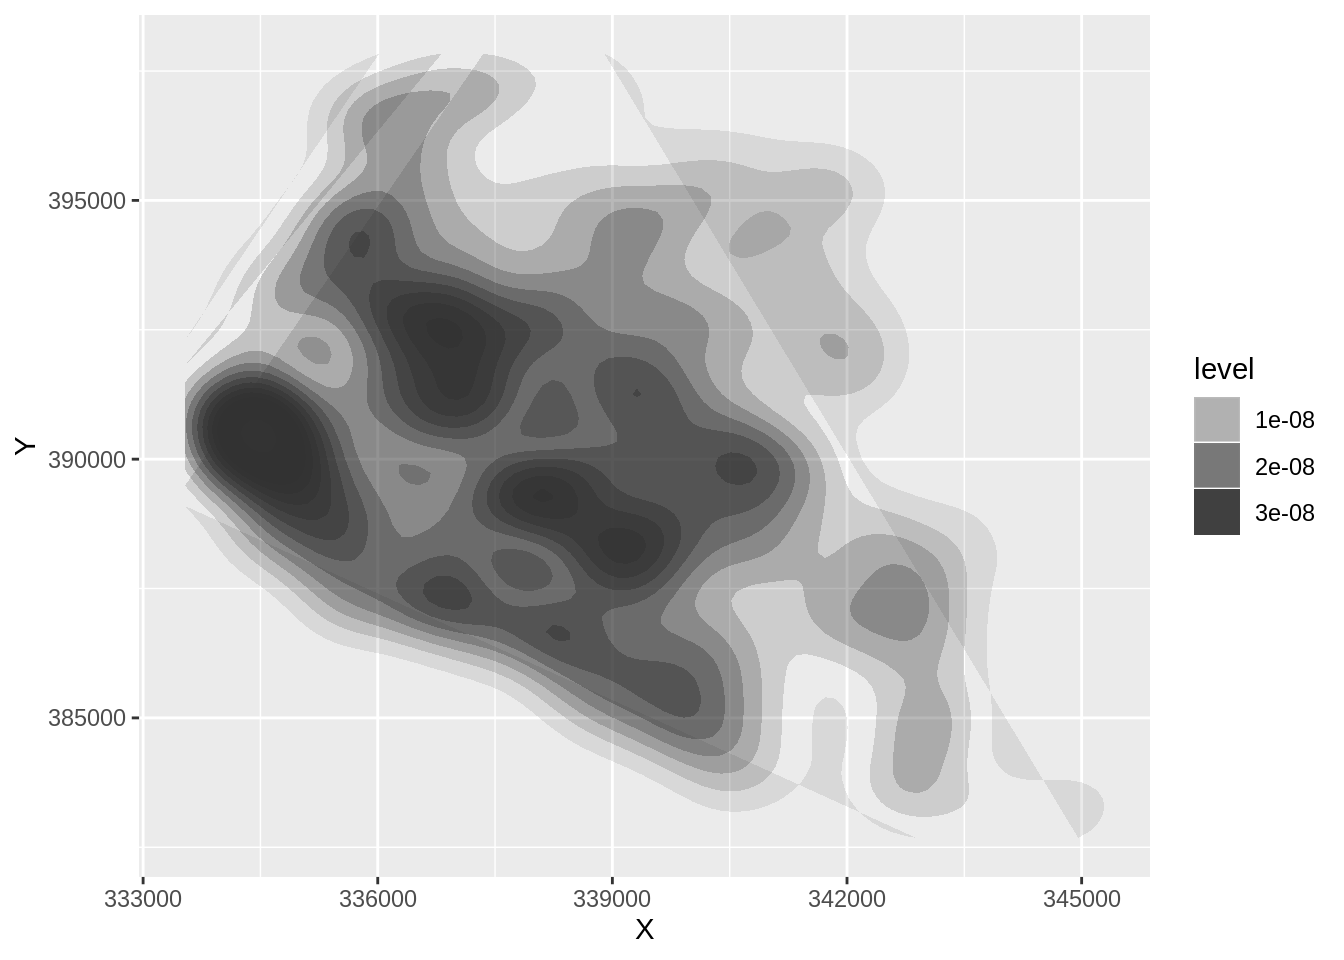
\includegraphics{05-flows_files/figure-pdf/unnamed-chunk-12-1.pdf}

Note how we transform the size so it's a proportion of the largest trip
and then it is compressed with a logarithm.

\section{Modelling flows}\label{modelling-flows}

Now we have an idea of the spatial distribution of flows, we can begin
to think about modeling them. The core idea in this section is to fit a
model that can capture the particular characteristics of our variable of
interest (the volume of trips) using a set of predictors that describe
the nature of a given flow. We will start from the simplest model and
then progressively build complexity until we get to a satisfying point.
Along the way, we will be exploring each model using concepts from
Gelman and Hill (2006) such as predictive performance checks\footnote{For
  a more elaborate introduction to PPC, have a look at Chapters 7 and 8.}
(PPC)

Before we start running regressions, let us first standardize the
predictors so we can interpret the intercept as the average flow when
all the predictors take the average value, and so we can interpret the
model coefficients as changes in standard deviation units:

\begin{Shaded}
\begin{Highlighting}[]
\CommentTok{\# Scale all the table}
\NormalTok{db\_std }\OtherTok{\textless{}{-}}\NormalTok{ db }\SpecialCharTok{\%\textgreater{}\%} \FunctionTok{mutate}\NormalTok{(}\FunctionTok{across}\NormalTok{(}\FunctionTok{where}\NormalTok{(is.numeric), scale))}

\CommentTok{\# Reset trips as we want the original version}
\NormalTok{db\_std}\SpecialCharTok{$}\NormalTok{trips15 }\OtherTok{\textless{}{-}}\NormalTok{ db}\SpecialCharTok{$}\NormalTok{trips15}
\NormalTok{db\_std}\SpecialCharTok{$}\NormalTok{trips16 }\OtherTok{\textless{}{-}}\NormalTok{ db}\SpecialCharTok{$}\NormalTok{trips16}

\CommentTok{\# Reset origin and destination station and express them as factors}
\NormalTok{db\_std}\SpecialCharTok{$}\NormalTok{orig }\OtherTok{\textless{}{-}} \FunctionTok{as.factor}\NormalTok{(db}\SpecialCharTok{$}\NormalTok{orig)}
\NormalTok{db\_std}\SpecialCharTok{$}\NormalTok{dest }\OtherTok{\textless{}{-}} \FunctionTok{as.factor}\NormalTok{(db}\SpecialCharTok{$}\NormalTok{dest)}
\end{Highlighting}
\end{Shaded}

\textbf{Baseline model}

One of the simplest possible models we can fit in this context is a
linear model that explains the number of trips as a function of the
straight distance between the two stations and total amount of climb and
downhill. We will take this as the baseline on which we can further
build later:

\begin{Shaded}
\begin{Highlighting}[]
\NormalTok{m1 }\OtherTok{\textless{}{-}} \FunctionTok{lm}\NormalTok{(}\StringTok{\textquotesingle{}trips15 \textasciitilde{} straight\_dist + total\_up + total\_down\textquotesingle{}}\NormalTok{, }\AttributeTok{data=}\NormalTok{db\_std)}
\FunctionTok{summary}\NormalTok{(m1)}
\end{Highlighting}
\end{Shaded}

\begin{verbatim}

Call:
lm(formula = "trips15 ~ straight_dist + total_up + total_down", 
    data = db_std)

Residuals:
   Min     1Q Median     3Q    Max 
-261.9 -168.3 -102.4   30.8 3527.4 

Coefficients:
              Estimate Std. Error t value Pr(>|t|)    
(Intercept)    182.070      8.110  22.451  < 2e-16 ***
straight_dist   17.906      9.108   1.966   0.0495 *  
total_up       -44.100      9.353  -4.715 2.61e-06 ***
total_down     -20.241      9.229  -2.193   0.0284 *  
---
Signif. codes:  0 '***' 0.001 '**' 0.01 '*' 0.05 '.' 0.1 ' ' 1

Residual standard error: 336.5 on 1718 degrees of freedom
Multiple R-squared:  0.02196,   Adjusted R-squared:  0.02025 
F-statistic: 12.86 on 3 and 1718 DF,  p-value: 2.625e-08
\end{verbatim}

To explore how good this model is, we will be comparing the predictions
the model makes about the number of trips each flow should have with the
actual number of trips. A first approach is to simply plot the
distribution of both variables:

\begin{Shaded}
\begin{Highlighting}[]
\FunctionTok{plot}\NormalTok{(}
  \FunctionTok{density}\NormalTok{( m1}\SpecialCharTok{$}\NormalTok{fitted.values ), }
  \AttributeTok{xlim =} \FunctionTok{c}\NormalTok{(}\SpecialCharTok{{-}}\DecValTok{100}\NormalTok{, }\FunctionTok{max}\NormalTok{( db\_std}\SpecialCharTok{$}\NormalTok{trips15 )),}
  \AttributeTok{main=}\StringTok{\textquotesingle{}\textquotesingle{}}
\NormalTok{)}
\FunctionTok{lines}\NormalTok{(}
  \FunctionTok{density}\NormalTok{( db\_std}\SpecialCharTok{$}\NormalTok{trips15 ), }
  \AttributeTok{col=}\StringTok{\textquotesingle{}red\textquotesingle{}}\NormalTok{,}
  \AttributeTok{main=}\StringTok{\textquotesingle{}\textquotesingle{}}
\NormalTok{)}
\FunctionTok{legend}\NormalTok{(}
  \StringTok{\textquotesingle{}topright\textquotesingle{}}\NormalTok{, }
  \FunctionTok{c}\NormalTok{(}\StringTok{\textquotesingle{}Predicted\textquotesingle{}}\NormalTok{, }\StringTok{\textquotesingle{}Actual\textquotesingle{}}\NormalTok{),}
  \AttributeTok{col=}\FunctionTok{c}\NormalTok{(}\StringTok{\textquotesingle{}black\textquotesingle{}}\NormalTok{, }\StringTok{\textquotesingle{}red\textquotesingle{}}\NormalTok{),}
  \AttributeTok{lwd=}\DecValTok{1}
\NormalTok{)}
\FunctionTok{title}\NormalTok{(}\AttributeTok{main=}\StringTok{"Predictive check, point estimates {-} Baseline model"}\NormalTok{)}
\end{Highlighting}
\end{Shaded}

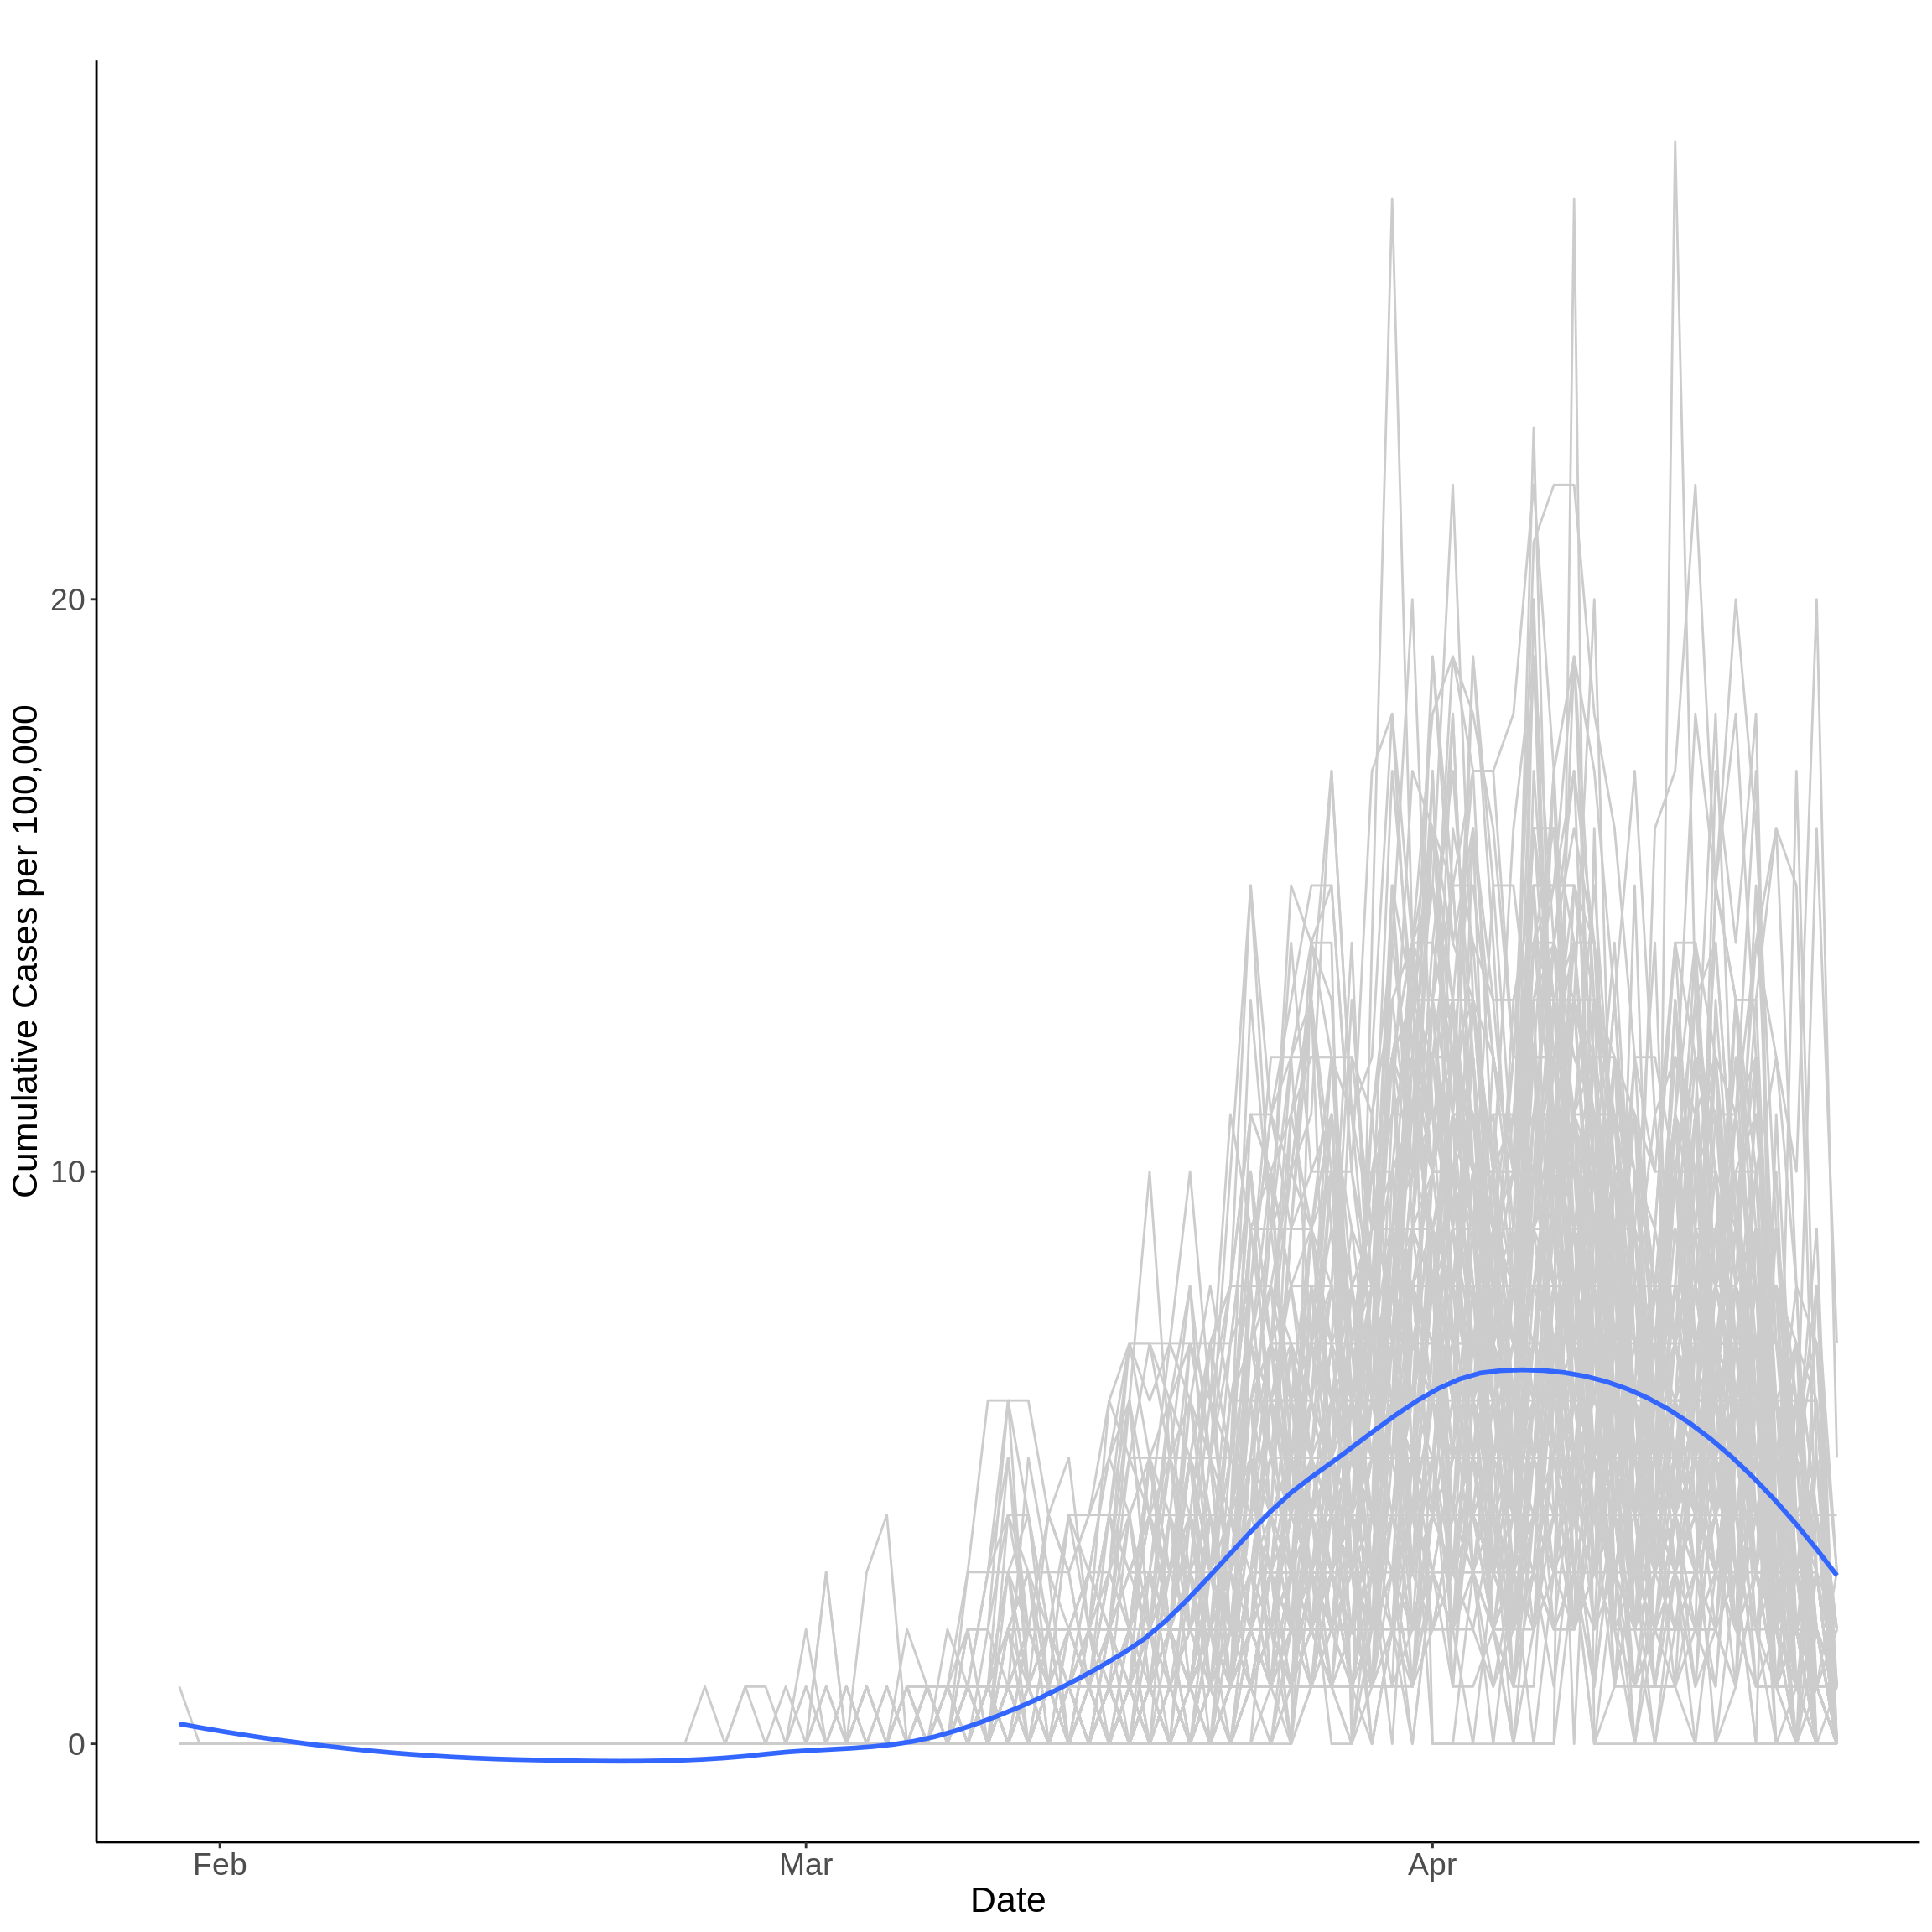
\includegraphics{05-flows_files/figure-pdf/unnamed-chunk-15-1.pdf}

The plot makes pretty obvious that our initial model captures very few
aspects of the distribution we want to explain. However, we should not
get too attached to this plot just yet. What it is showing is the
distribution of predicted \emph{point} estimates from our model. Since
our model is not deterministic but inferential, there is a certain
degree of uncertainty attached to its predictions, and that is
completely absent from this plot.

Generally speaking, a given model has two sources of uncertainty:
\emph{predictive}, and \emph{inferential}. The former relates to the
fact that the equation we fit does not capture all the elements or in
the exact form they enter the true data generating process; the latter
has to do with the fact that we never get to know the true value of the
model parameters only guesses (estimates) subject to error and
uncertainty. If you think of our linear model above as

\[
T_{ij} = X_{ij}\beta + \epsilon_{ij}
\] where \(T_{ij}\) represents the number of trips undertaken between
station \(i\) and \(j\), \(X_{ij}\) is the set of explanatory variables
(length, climb, descent, etc.), and \(\epsilon_{ij}\) is an error term
assumed to be distributed as a normal distribution \(N(0, \sigma)\);
then predictive uncertainty comes from the fact that there are elements
to some extent relevant for \(y\) that are not accounted for and thus
subsummed into \(\epsilon_{ij}\). Inferential uncertainty comes from the
fact that we never get to know \(\beta\) but only an estimate of it
which is also subject to uncertainty itself.

Taking these two sources into consideration means that the black line in
the plot above represents only the behaviour of our model we expect if
the error term is absent (no predictive uncertainty) and the
coefficients are the true estimates (no inferential uncertainty).
However, this is not necessarily the case as our estimate for the
uncertainty of the error term is certainly not zero, and our estimates
for each parameter are also subject to a great deal of inferential
variability. We do not know to what extent other outcomes would be just
as likely. Predictive checking relates to simulating several feasible
scenarios under our model and use those to assess uncertainty and to get
a better grasp of the quality of our predictions.

Technically speaking, to do this, we need to build a mechanism to obtain
a possible draw from our model and then repeat it several times. The
first part of those two steps can be elegantly dealt with by writing a
short function that takes a given model and a set of predictors, and
produces a possible random draw from such model:

\begin{Shaded}
\begin{Highlighting}[]
\NormalTok{generate\_draw }\OtherTok{\textless{}{-}} \ControlFlowTok{function}\NormalTok{(m)\{}
  \CommentTok{\# Set up predictors matrix}
\NormalTok{  x }\OtherTok{\textless{}{-}} \FunctionTok{model.matrix}\NormalTok{( m )}
  \CommentTok{\# Obtain draws of parameters (inferential uncertainty)}
\NormalTok{  sim\_bs }\OtherTok{\textless{}{-}} \FunctionTok{sim}\NormalTok{( m, }\DecValTok{1}\NormalTok{)}
  \CommentTok{\# Predicted value}
\NormalTok{  mu }\OtherTok{\textless{}{-}}\NormalTok{ x }\SpecialCharTok{\%*\%}\NormalTok{ sim\_bs}\SpecialCharTok{@}\NormalTok{coef[}\DecValTok{1}\NormalTok{, ]}
  \CommentTok{\# Draw}
\NormalTok{  n }\OtherTok{\textless{}{-}} \FunctionTok{length}\NormalTok{( mu )}
\NormalTok{  y\_hat }\OtherTok{\textless{}{-}} \FunctionTok{rnorm}\NormalTok{( n, mu, sim\_bs}\SpecialCharTok{@}\NormalTok{sigma[}\DecValTok{1}\NormalTok{])}
  \FunctionTok{return}\NormalTok{(y\_hat)}
\NormalTok{\}}
\end{Highlighting}
\end{Shaded}

This function takes a model \texttt{m} and the set of covariates
\texttt{x} used and returns a random realization of predictions from the
model. To get a sense of how this works, we can get and plot a
realization of the model, compared to the expected one and the actual
values:

\begin{Shaded}
\begin{Highlighting}[]
\NormalTok{new\_y }\OtherTok{\textless{}{-}} \FunctionTok{generate\_draw}\NormalTok{(m1)}

\FunctionTok{plot}\NormalTok{(}
  \FunctionTok{density}\NormalTok{( m1}\SpecialCharTok{$}\NormalTok{fitted.values ), }
  \AttributeTok{xlim =} \FunctionTok{c}\NormalTok{(}\SpecialCharTok{{-}}\DecValTok{100}\NormalTok{, }\FunctionTok{max}\NormalTok{( db\_std}\SpecialCharTok{$}\NormalTok{trips15 )),}
  \AttributeTok{ylim =} \FunctionTok{c}\NormalTok{(}\DecValTok{0}\NormalTok{, }\FunctionTok{max}\NormalTok{(}\FunctionTok{c}\NormalTok{(}
                   \FunctionTok{max}\NormalTok{( }\FunctionTok{density}\NormalTok{( m1}\SpecialCharTok{$}\NormalTok{fitted.values)}\SpecialCharTok{$}\NormalTok{y ), }
                   \FunctionTok{max}\NormalTok{( }\FunctionTok{density}\NormalTok{( db\_std}\SpecialCharTok{$}\NormalTok{trips15)}\SpecialCharTok{$}\NormalTok{y )}
\NormalTok{                   )}
\NormalTok{                )}
\NormalTok{         ),}
  \AttributeTok{col =} \StringTok{\textquotesingle{}black\textquotesingle{}}\NormalTok{,}
  \AttributeTok{main =} \StringTok{\textquotesingle{}\textquotesingle{}}
\NormalTok{)}
\FunctionTok{lines}\NormalTok{(}
  \FunctionTok{density}\NormalTok{( db\_std}\SpecialCharTok{$}\NormalTok{trips15 ), }
  \AttributeTok{col =} \StringTok{\textquotesingle{}red\textquotesingle{}}\NormalTok{,}
  \AttributeTok{main =} \StringTok{\textquotesingle{}\textquotesingle{}}
\NormalTok{)}
\FunctionTok{lines}\NormalTok{(}
  \FunctionTok{density}\NormalTok{( new\_y ), }
  \AttributeTok{col =} \StringTok{\textquotesingle{}green\textquotesingle{}}\NormalTok{,}
  \AttributeTok{main =} \StringTok{\textquotesingle{}\textquotesingle{}}
\NormalTok{)}
\FunctionTok{legend}\NormalTok{(}
  \StringTok{\textquotesingle{}topright\textquotesingle{}}\NormalTok{, }
  \FunctionTok{c}\NormalTok{(}\StringTok{\textquotesingle{}Predicted\textquotesingle{}}\NormalTok{, }\StringTok{\textquotesingle{}Actual\textquotesingle{}}\NormalTok{, }\StringTok{\textquotesingle{}Simulated\textquotesingle{}}\NormalTok{),}
  \AttributeTok{col =} \FunctionTok{c}\NormalTok{( }\StringTok{\textquotesingle{}black\textquotesingle{}}\NormalTok{, }\StringTok{\textquotesingle{}red\textquotesingle{}}\NormalTok{, }\StringTok{\textquotesingle{}green\textquotesingle{}}\NormalTok{ ),}
  \AttributeTok{lwd =} \DecValTok{1}
\NormalTok{)}
\end{Highlighting}
\end{Shaded}

\includegraphics{05-flows_files/figure-pdf/unnamed-chunk-17-1.pdf}

Once we have this ``draw engine'', we can set it to work as many times
as we want using a simple \texttt{for} loop. In fact, we can directly
plot these lines as compared to the expected one and the trip count:

\begin{Shaded}
\begin{Highlighting}[]
\FunctionTok{plot}\NormalTok{(}
  \FunctionTok{density}\NormalTok{( m1}\SpecialCharTok{$}\NormalTok{fitted.values ), }
  \AttributeTok{xlim =} \FunctionTok{c}\NormalTok{(}\SpecialCharTok{{-}}\DecValTok{100}\NormalTok{, }\FunctionTok{max}\NormalTok{( db\_std}\SpecialCharTok{$}\NormalTok{trips15 )),}
  \AttributeTok{ylim =} \FunctionTok{c}\NormalTok{(}\DecValTok{0}\NormalTok{, }\FunctionTok{max}\NormalTok{(}\FunctionTok{c}\NormalTok{(}
               \FunctionTok{max}\NormalTok{( }\FunctionTok{density}\NormalTok{( m1}\SpecialCharTok{$}\NormalTok{fitted.values)}\SpecialCharTok{$}\NormalTok{y ), }
               \FunctionTok{max}\NormalTok{( }\FunctionTok{density}\NormalTok{( db\_std}\SpecialCharTok{$}\NormalTok{trips15)}\SpecialCharTok{$}\NormalTok{y )}
\NormalTok{               )}
\NormalTok{            )}
\NormalTok{     ),}
  \AttributeTok{col=}\StringTok{\textquotesingle{}white\textquotesingle{}}\NormalTok{,}
  \AttributeTok{main=}\StringTok{\textquotesingle{}\textquotesingle{}}
\NormalTok{)}
\CommentTok{\# Loop for realizations}
\ControlFlowTok{for}\NormalTok{(i }\ControlFlowTok{in} \DecValTok{1}\SpecialCharTok{:}\DecValTok{250}\NormalTok{)\{}
\NormalTok{  tmp\_y }\OtherTok{\textless{}{-}} \FunctionTok{generate\_draw}\NormalTok{( m1 )}
  \FunctionTok{lines}\NormalTok{( }\FunctionTok{density}\NormalTok{( tmp\_y ),}
        \AttributeTok{col =} \StringTok{\textquotesingle{}grey\textquotesingle{}}\NormalTok{,}
        \AttributeTok{lwd =} \FloatTok{0.1}
\NormalTok{        )}
\NormalTok{\}}
\CommentTok{\#}
\FunctionTok{lines}\NormalTok{(}
  \FunctionTok{density}\NormalTok{( m1}\SpecialCharTok{$}\NormalTok{fitted.values ), }
  \AttributeTok{col =} \StringTok{\textquotesingle{}black\textquotesingle{}}\NormalTok{,}
  \AttributeTok{main =} \StringTok{\textquotesingle{}\textquotesingle{}}
\NormalTok{)}
\FunctionTok{lines}\NormalTok{(}
  \FunctionTok{density}\NormalTok{( db\_std}\SpecialCharTok{$}\NormalTok{trips15 ), }
  \AttributeTok{col =} \StringTok{\textquotesingle{}red\textquotesingle{}}\NormalTok{,}
  \AttributeTok{main =} \StringTok{\textquotesingle{}\textquotesingle{}}
\NormalTok{)}
\FunctionTok{legend}\NormalTok{(}
  \StringTok{\textquotesingle{}topright\textquotesingle{}}\NormalTok{, }
  \FunctionTok{c}\NormalTok{(}\StringTok{\textquotesingle{}Actual\textquotesingle{}}\NormalTok{, }\StringTok{\textquotesingle{}Predicted\textquotesingle{}}\NormalTok{, }\StringTok{\textquotesingle{}Simulated (n=250)\textquotesingle{}}\NormalTok{),}
  \AttributeTok{col =} \FunctionTok{c}\NormalTok{(}\StringTok{\textquotesingle{}red\textquotesingle{}}\NormalTok{, }\StringTok{\textquotesingle{}black\textquotesingle{}}\NormalTok{, }\StringTok{\textquotesingle{}grey\textquotesingle{}}\NormalTok{),}
  \AttributeTok{lwd =} \DecValTok{1}
\NormalTok{)}
\FunctionTok{title}\NormalTok{(}\AttributeTok{main=}\StringTok{"Predictive check {-} Baseline model"}\NormalTok{)}
\end{Highlighting}
\end{Shaded}

\includegraphics{05-flows_files/figure-pdf/unnamed-chunk-18-1.pdf}

The plot shows there is a significant mismatch between the fitted
values, which are much more concentrated around small positive values,
and the realizations of our ``inferential engine'', which depict a much
less concentrated distribution of values. This is likely due to the
combination of two different reasons: on the one hand, the accuracy of
our estimates may be poor, causing them to jump around a wide range of
potential values and hence resulting in very diverse predictions
(inferential uncertainty); on the other hand, it may be that the amount
of variation we are not able to account for in the model\footnote{The
  \(R^2\) of our model is around 2\%} is so large that the degree of
uncertainty contained in the error term of the model is very large,
hence resulting in such a flat predictive distribution.

It is important to keep in mind that the issues discussed in the
paragraph above relate only to the uncertainty behind our model, not to
the point predictions derived from them, which are a mechanistic result
of the minimization of the squared residuals and hence are not subject
to probability or inference. That allows them in this case to provide a
fitted distribution much more accurate apparently (black line above).
However, the lesson to take from this model is that, even if the point
predictions (fitted values) are artificially accurate\footnote{which
  they are not really, in light of the comparison between the black and
  red lines.}, our capabilities to infer about the more general
underlying process are fairly limited.

\textbf{Improving the model}

The bad news from the previous section is that our initial model is not
great at explaining bike trips. The good news is there are several ways
in which we can improve this. In this section we will cover three main
extensions that exemplify three different routes you can take when
enriching and augmenting models in general, and spatial interaction ones
in particular\footnote{These principles are general and can be applied
  to pretty much any modeling exercise you run into. The specific
  approaches we take in this note relate to spatial interaction models}.
These three routes are aligned around the following principles:

\begin{enumerate}
\def\labelenumi{\arabic{enumi}.}
\tightlist
\item
  Use better approximations to model your dependent variable.
\item
  Recognize the structure of your data.
\item
  Get better predictors.
\end{enumerate}

\begin{itemize}
\tightlist
\item
  \textbf{Use better approximations to model your dependent variable}
\end{itemize}

Standard OLS regression assumes that the error term and, since the
predictors are deterministic, the dependent variable are distributed
following a normal (gaussian) distribution. This is usually a good
approximation for several phenomena of interest, but maybe not the best
one for trips along routes: for one, we know trips cannot be negative,
which the normal distribution does not account for\footnote{For an
  illustration of this, consider the amount of probability mass to the
  left of zero in the predictive checks above.}; more subtly, their
distribution is not really symmetric but skewed with a very long tail on
the right. This is common in variables that represent counts and that is
why usually it is more appropriate to fit a model that relies on a
distribution different from the normal.

One of the most common distributions for this cases is the Poisson,
which can be incorporated through a general linear model (or GLM). The
underlying assumption here is that instead of
\(T_{ij} \sim N(\mu_{ij}, \sigma)\), our model now follows:

\[
T_{ij} \sim Poisson (\exp^{X_{ij}\beta})
\]

As usual, such a model is easy to run in R:

\begin{Shaded}
\begin{Highlighting}[]
\NormalTok{m2 }\OtherTok{\textless{}{-}} \FunctionTok{glm}\NormalTok{(}
  \StringTok{\textquotesingle{}trips15 \textasciitilde{} straight\_dist + total\_up + total\_down\textquotesingle{}}\NormalTok{, }
  \AttributeTok{data=}\NormalTok{db\_std,}
  \AttributeTok{family=}\NormalTok{poisson,}
\NormalTok{)}
\end{Highlighting}
\end{Shaded}

Now let's see how much better, if any, this approach is. To get a quick
overview, we can simply plot the point predictions:

\begin{Shaded}
\begin{Highlighting}[]
\FunctionTok{plot}\NormalTok{(}
  \FunctionTok{density}\NormalTok{( m2}\SpecialCharTok{$}\NormalTok{fitted.values ), }
  \AttributeTok{xlim =} \FunctionTok{c}\NormalTok{( }\SpecialCharTok{{-}}\DecValTok{100}\NormalTok{, }\FunctionTok{max}\NormalTok{( db\_std}\SpecialCharTok{$}\NormalTok{trips15 )),}
  \AttributeTok{ylim =} \FunctionTok{c}\NormalTok{( }\DecValTok{0}\NormalTok{, }\FunctionTok{max}\NormalTok{(}\FunctionTok{c}\NormalTok{(}
               \FunctionTok{max}\NormalTok{( }\FunctionTok{density}\NormalTok{( m2}\SpecialCharTok{$}\NormalTok{fitted.values)}\SpecialCharTok{$}\NormalTok{y ), }
               \FunctionTok{max}\NormalTok{( }\FunctionTok{density}\NormalTok{(db\_std}\SpecialCharTok{$}\NormalTok{trips15)}\SpecialCharTok{$}\NormalTok{y )}
\NormalTok{               )}
\NormalTok{            )}
\NormalTok{   ),}
  \AttributeTok{col =} \StringTok{\textquotesingle{}black\textquotesingle{}}\NormalTok{,}
  \AttributeTok{main =} \StringTok{\textquotesingle{}\textquotesingle{}}
\NormalTok{)}
\FunctionTok{lines}\NormalTok{(}
  \FunctionTok{density}\NormalTok{( db\_std}\SpecialCharTok{$}\NormalTok{trips15 ), }
  \AttributeTok{col =} \StringTok{\textquotesingle{}red\textquotesingle{}}\NormalTok{,}
  \AttributeTok{main =} \StringTok{\textquotesingle{}\textquotesingle{}}
\NormalTok{)}
\FunctionTok{legend}\NormalTok{(}
  \StringTok{\textquotesingle{}topright\textquotesingle{}}\NormalTok{, }
  \FunctionTok{c}\NormalTok{(}\StringTok{\textquotesingle{}Predicted\textquotesingle{}}\NormalTok{, }\StringTok{\textquotesingle{}Actual\textquotesingle{}}\NormalTok{),}
  \AttributeTok{col =} \FunctionTok{c}\NormalTok{(}\StringTok{\textquotesingle{}black\textquotesingle{}}\NormalTok{, }\StringTok{\textquotesingle{}red\textquotesingle{}}\NormalTok{),}
  \AttributeTok{lwd =} \DecValTok{1}
\NormalTok{)}
\FunctionTok{title}\NormalTok{(}\AttributeTok{main =} \StringTok{"Predictive check, point estimates {-} Poisson model"}\NormalTok{)}
\end{Highlighting}
\end{Shaded}

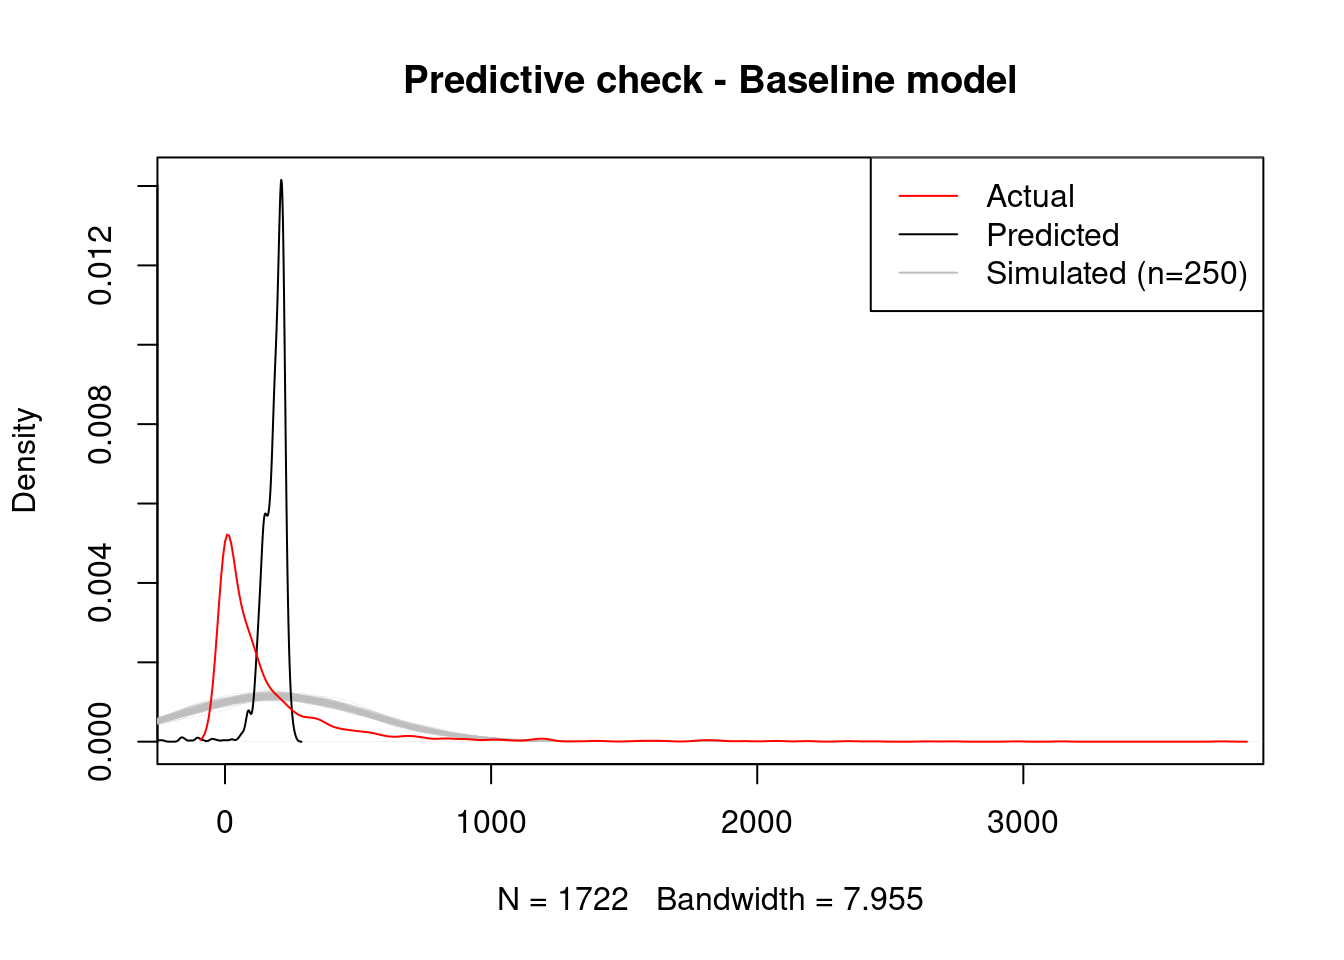
\includegraphics{05-flows_files/figure-pdf/unnamed-chunk-20-1.pdf}

To incorporate uncertainty to these predictions, we need to tweak our
\texttt{generate\_draw} function so it accommodates the fact that our
model is not linear anymore.

\begin{Shaded}
\begin{Highlighting}[]
\NormalTok{generate\_draw\_poi }\OtherTok{\textless{}{-}} \ControlFlowTok{function}\NormalTok{(m)\{}
  \CommentTok{\# Set up predictors matrix}
\NormalTok{  x }\OtherTok{\textless{}{-}} \FunctionTok{model.matrix}\NormalTok{( m )}
  \CommentTok{\# Obtain draws of parameters (inferential uncertainty)}
\NormalTok{  sim\_bs }\OtherTok{\textless{}{-}} \FunctionTok{sim}\NormalTok{( m, }\DecValTok{1}\NormalTok{ )}
  \CommentTok{\# Predicted value}
\NormalTok{  xb }\OtherTok{\textless{}{-}}\NormalTok{ x }\SpecialCharTok{\%*\%}\NormalTok{ sim\_bs}\SpecialCharTok{@}\NormalTok{coef[}\DecValTok{1}\NormalTok{, ]}
  \CommentTok{\#xb \textless{}{-} x \%*\% m$coefficients}
  \CommentTok{\# Transform using the link function}
\NormalTok{  mu }\OtherTok{\textless{}{-}} \FunctionTok{exp}\NormalTok{( xb )}
  \CommentTok{\# Obtain a random realization}
\NormalTok{  y\_hat }\OtherTok{\textless{}{-}} \FunctionTok{rpois}\NormalTok{( }\AttributeTok{n =} \FunctionTok{length}\NormalTok{( mu ), }\AttributeTok{lambda =}\NormalTok{ mu)}
  \FunctionTok{return}\NormalTok{(y\_hat)}
\NormalTok{\}}
\end{Highlighting}
\end{Shaded}

And then we can examine both point predictions an uncertainty around
them:

\begin{Shaded}
\begin{Highlighting}[]
\FunctionTok{plot}\NormalTok{(}
  \FunctionTok{density}\NormalTok{( m2}\SpecialCharTok{$}\NormalTok{fitted.values ), }
  \AttributeTok{xlim =} \FunctionTok{c}\NormalTok{(}\SpecialCharTok{{-}}\DecValTok{100}\NormalTok{, }\FunctionTok{max}\NormalTok{( db\_std}\SpecialCharTok{$}\NormalTok{trips15 )),}
  \AttributeTok{ylim =} \FunctionTok{c}\NormalTok{(}\DecValTok{0}\NormalTok{, }\FunctionTok{max}\NormalTok{(}\FunctionTok{c}\NormalTok{(}
               \FunctionTok{max}\NormalTok{( }\FunctionTok{density}\NormalTok{( m2}\SpecialCharTok{$}\NormalTok{fitted.values)}\SpecialCharTok{$}\NormalTok{y ), }
               \FunctionTok{max}\NormalTok{( }\FunctionTok{density}\NormalTok{( db\_std}\SpecialCharTok{$}\NormalTok{trips15)}\SpecialCharTok{$}\NormalTok{y )}
\NormalTok{               )}
\NormalTok{            )}
\NormalTok{   ),}
  \AttributeTok{col =} \StringTok{\textquotesingle{}white\textquotesingle{}}\NormalTok{,}
  \AttributeTok{main =} \StringTok{\textquotesingle{}\textquotesingle{}}
\NormalTok{)}
\CommentTok{\# Loop for realizations}
\ControlFlowTok{for}\NormalTok{(i }\ControlFlowTok{in} \DecValTok{1}\SpecialCharTok{:}\DecValTok{250}\NormalTok{)\{}
\NormalTok{  tmp\_y }\OtherTok{\textless{}{-}} \FunctionTok{generate\_draw\_poi}\NormalTok{( m2 )}
  \FunctionTok{lines}\NormalTok{(}
    \FunctionTok{density}\NormalTok{( tmp\_y ),}
    \AttributeTok{col =} \StringTok{\textquotesingle{}grey\textquotesingle{}}\NormalTok{,}
    \AttributeTok{lwd =} \FloatTok{0.1}
\NormalTok{  )}
\NormalTok{\}}
\CommentTok{\#}
\FunctionTok{lines}\NormalTok{(}
  \FunctionTok{density}\NormalTok{( m2}\SpecialCharTok{$}\NormalTok{fitted.values ), }
  \AttributeTok{col =} \StringTok{\textquotesingle{}black\textquotesingle{}}\NormalTok{,}
  \AttributeTok{main =} \StringTok{\textquotesingle{}\textquotesingle{}}
\NormalTok{)}
\FunctionTok{lines}\NormalTok{(}
  \FunctionTok{density}\NormalTok{( db\_std}\SpecialCharTok{$}\NormalTok{trips15 ), }
  \AttributeTok{col =} \StringTok{\textquotesingle{}red\textquotesingle{}}\NormalTok{,}
  \AttributeTok{main =} \StringTok{\textquotesingle{}\textquotesingle{}}
\NormalTok{)}
\FunctionTok{legend}\NormalTok{(}
  \StringTok{\textquotesingle{}topright\textquotesingle{}}\NormalTok{, }
  \FunctionTok{c}\NormalTok{(}\StringTok{\textquotesingle{}Predicted\textquotesingle{}}\NormalTok{, }\StringTok{\textquotesingle{}Actual\textquotesingle{}}\NormalTok{, }\StringTok{\textquotesingle{}Simulated (n=250)\textquotesingle{}}\NormalTok{),}
  \AttributeTok{col =} \FunctionTok{c}\NormalTok{(}\StringTok{\textquotesingle{}black\textquotesingle{}}\NormalTok{, }\StringTok{\textquotesingle{}red\textquotesingle{}}\NormalTok{, }\StringTok{\textquotesingle{}grey\textquotesingle{}}\NormalTok{),}
  \AttributeTok{lwd =} \DecValTok{1}
\NormalTok{)}
\FunctionTok{title}\NormalTok{( }\AttributeTok{main =} \StringTok{"Predictive check {-} Poisson model"}\NormalTok{)}
\end{Highlighting}
\end{Shaded}

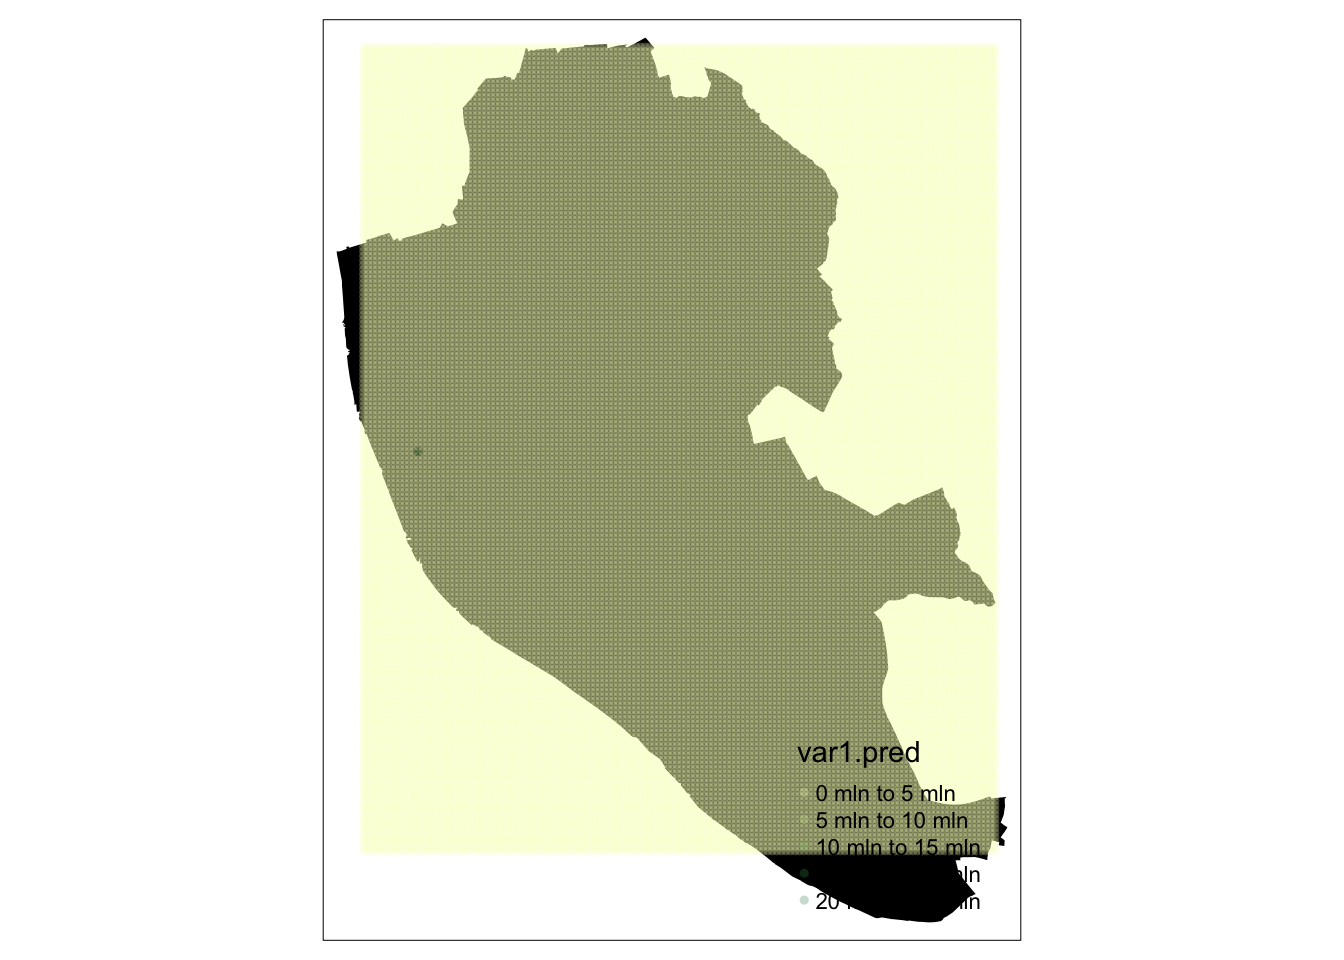
\includegraphics{05-flows_files/figure-pdf/unnamed-chunk-22-1.pdf}

Voila! Although the curve is still a bit off, centered too much to the
right of the actual data, our predictive simulation leaves the fitted
values right in the middle. This speaks to a better fit of the model to
the actual distribution othe original data follow.

\begin{itemize}
\tightlist
\item
  \textbf{Recognize the structure of your data}
\end{itemize}

So far, we've treated our dataset as if it was flat (i.e.~comprise of
fully independent realizations) when in fact it is not. Most crucially,
our baseline model does not account for the fact that every observation
in the dataset pertains to a trip between two stations. This means that
all the trips from or to the same station probably share elements which
likely help explain how many trips are undertaken between stations. For
example, think of trips to and from a station located in the famous
Embarcadero, a popular tourist spot. Every route to and from there
probably has more trips due to the popularity of the area and we are
currently not acknowledging it in the model.

A simple way to incorporate these effects into the model is through
origin and destination fixed effects. This approach shares elements with
both spatial fixed effects and multilevel modeling and essentially
consists of including a binary variable for every origin and destination
station. In mathematical notation, this equates to:

\[
T_{ij} = X_{ij}\beta + \delta_i + \delta_j + \epsilon_{ij}
\]

where \(\delta_i\) and \(\delta_j\) are origin and destination station
fixed effects\footnote{In this session, \(\delta_i\) and \(\delta_j\)
  are estimated as independent variables so their estimates are similar
  to interpret to those in \(\beta\). An alternative approach could be
  to model them as random effects in a multilevel framework.}, and the
rest is as above. This strategy accounts for all the unobserved
heterogeneity associated with the location of the station. Technically
speaking, we simply need to introduce \texttt{orig} and \texttt{dest} in
the the model:

\begin{Shaded}
\begin{Highlighting}[]
\NormalTok{m3 }\OtherTok{\textless{}{-}} \FunctionTok{glm}\NormalTok{(}
  \StringTok{\textquotesingle{}trips15 \textasciitilde{} straight\_dist + total\_up + total\_down + orig + dest\textquotesingle{}}\NormalTok{, }
  \AttributeTok{data =}\NormalTok{ db\_std,}
  \AttributeTok{family =}\NormalTok{ poisson}
\NormalTok{)}
\end{Highlighting}
\end{Shaded}

And with our new model, we can have a look at how well it does at
predicting the overall number of trips\footnote{Although, theoretically,
  we could also include simulations of the model in the plot to get a
  better sense of the uncertainty behind our model, in practice this
  seems troublesome. The problems most likely arise from the fact that
  many of the origin and destination binary variable coefficients are
  estimated with a great deal of uncertainty. This causes some of the
  simulation to generate extreme values that, when passed through the
  exponential term of the Poisson link function, cause problems. If
  anything, this is testimony of how a simple fixed effect model can
  sometimes lack accuracy and generate very uncertain estimates. A
  potential extension to work around these problems could be to fit a
  multilevel model with two specific levels beyond the trip-level: one
  for origin and another one for destination stations.}:

\begin{Shaded}
\begin{Highlighting}[]
\FunctionTok{plot}\NormalTok{(}
  \FunctionTok{density}\NormalTok{( m3}\SpecialCharTok{$}\NormalTok{fitted.values ), }
  \AttributeTok{xlim =} \FunctionTok{c}\NormalTok{(}\SpecialCharTok{{-}}\DecValTok{100}\NormalTok{, }\FunctionTok{max}\NormalTok{( db\_std}\SpecialCharTok{$}\NormalTok{trips15 )),}
  \AttributeTok{ylim =} \FunctionTok{c}\NormalTok{(}\DecValTok{0}\NormalTok{, }\FunctionTok{max}\NormalTok{(}\FunctionTok{c}\NormalTok{(}
               \FunctionTok{max}\NormalTok{( }\FunctionTok{density}\NormalTok{(m3}\SpecialCharTok{$}\NormalTok{fitted.values)}\SpecialCharTok{$}\NormalTok{y ), }
               \FunctionTok{max}\NormalTok{( }\FunctionTok{density}\NormalTok{(db\_std}\SpecialCharTok{$}\NormalTok{trips15)}\SpecialCharTok{$}\NormalTok{y )}
\NormalTok{               )}
\NormalTok{            )}
\NormalTok{   ),}
  \AttributeTok{col =} \StringTok{\textquotesingle{}black\textquotesingle{}}\NormalTok{,}
  \AttributeTok{main =} \StringTok{\textquotesingle{}\textquotesingle{}}
\NormalTok{)}
\FunctionTok{lines}\NormalTok{(}
  \FunctionTok{density}\NormalTok{( db\_std}\SpecialCharTok{$}\NormalTok{trips15 ), }
  \AttributeTok{col =} \StringTok{\textquotesingle{}red\textquotesingle{}}\NormalTok{,}
  \AttributeTok{main =} \StringTok{\textquotesingle{}\textquotesingle{}}
\NormalTok{)}
\FunctionTok{legend}\NormalTok{(}
  \StringTok{\textquotesingle{}topright\textquotesingle{}}\NormalTok{, }
  \FunctionTok{c}\NormalTok{(}\StringTok{\textquotesingle{}Predicted\textquotesingle{}}\NormalTok{, }\StringTok{\textquotesingle{}Actual\textquotesingle{}}\NormalTok{),}
  \AttributeTok{col =} \FunctionTok{c}\NormalTok{(}\StringTok{\textquotesingle{}black\textquotesingle{}}\NormalTok{, }\StringTok{\textquotesingle{}red\textquotesingle{}}\NormalTok{),}
  \AttributeTok{lwd =} \DecValTok{1}
\NormalTok{)}
\FunctionTok{title}\NormalTok{( }\AttributeTok{main =} \StringTok{"Predictive check {-} Orig/dest FE Poisson model"}\NormalTok{)}
\end{Highlighting}
\end{Shaded}

\includegraphics{05-flows_files/figure-pdf/unnamed-chunk-24-1.pdf}

That looks significantly better, doesn't it? In fact, our model now
better accounts for the long tail where a few routes take a lot of
trips. This is likely because the distribution of trips is far from
random across stations and our origin and destination fixed effects do a
decent job at accounting for that structure. However our model is still
notably underpredicting less popular routes and overpredicting routes
with above average number of trips. Maybe we should think about moving
beyond a simple linear model.

\begin{itemize}
\tightlist
\item
  \textbf{Get better predictors}
\end{itemize}

The final extension is, in principle, always available but, in practice,
it can be tricky to implement. The core idea is that your baseline model
might not have the best measurement of the phenomena you want to account
for. In our example, we can think of the distance between stations. So
far, we have been including the distance measured ``as the crow flies''
between stations. Although in some cases this is a good approximation
(particularly when distances are long and likely route taken is as close
to straight as possible), in some cases like ours, where the street
layout and the presence of elevation probably matter more than the
actual final distance pedalled, this is not necessarily a safe
assumption.

As an exampe of this approach, we can replace the straight distance
measurements for more refined ones based on the Google Maps API routes.
This is very easy as all we need to do (once the distances have been
calculated!) is to swap \texttt{straight\_dist} for
\texttt{street\_dist}:

\begin{Shaded}
\begin{Highlighting}[]
\NormalTok{m4 }\OtherTok{\textless{}{-}} \FunctionTok{glm}\NormalTok{(}
  \StringTok{\textquotesingle{}trips15 \textasciitilde{} street\_dist + total\_up + total\_down + orig + dest\textquotesingle{}}\NormalTok{, }
  \AttributeTok{data =}\NormalTok{ db\_std,}
  \AttributeTok{family =}\NormalTok{ poisson}
\NormalTok{)}
\end{Highlighting}
\end{Shaded}

And we can similarly get a sense of our predictive fitting with:

\begin{Shaded}
\begin{Highlighting}[]
\FunctionTok{plot}\NormalTok{(}
  \FunctionTok{density}\NormalTok{( m4}\SpecialCharTok{$}\NormalTok{fitted.values ), }
  \AttributeTok{xlim =} \FunctionTok{c}\NormalTok{(}\SpecialCharTok{{-}}\DecValTok{100}\NormalTok{, }\FunctionTok{max}\NormalTok{( db\_std}\SpecialCharTok{$}\NormalTok{trips15)),}
  \AttributeTok{ylim =} \FunctionTok{c}\NormalTok{(}\DecValTok{0}\NormalTok{, }\FunctionTok{max}\NormalTok{(}\FunctionTok{c}\NormalTok{(}
               \FunctionTok{max}\NormalTok{( }\FunctionTok{density}\NormalTok{(m4}\SpecialCharTok{$}\NormalTok{fitted.values)}\SpecialCharTok{$}\NormalTok{y ), }
               \FunctionTok{max}\NormalTok{( }\FunctionTok{density}\NormalTok{(db\_std}\SpecialCharTok{$}\NormalTok{trips15)}\SpecialCharTok{$}\NormalTok{y )}
\NormalTok{               )}
\NormalTok{            )}
\NormalTok{   ),}
  \AttributeTok{col =} \StringTok{\textquotesingle{}black\textquotesingle{}}\NormalTok{,}
  \AttributeTok{main =} \StringTok{\textquotesingle{}\textquotesingle{}}
\NormalTok{)}
\FunctionTok{lines}\NormalTok{(}
  \FunctionTok{density}\NormalTok{( db\_std}\SpecialCharTok{$}\NormalTok{trips15 ), }
  \AttributeTok{col =} \StringTok{\textquotesingle{}red\textquotesingle{}}\NormalTok{,}
  \AttributeTok{main =} \StringTok{\textquotesingle{}\textquotesingle{}}
\NormalTok{)}
\FunctionTok{legend}\NormalTok{(}
  \StringTok{\textquotesingle{}topright\textquotesingle{}}\NormalTok{, }
  \FunctionTok{c}\NormalTok{(}\StringTok{\textquotesingle{}Predicted\textquotesingle{}}\NormalTok{, }\StringTok{\textquotesingle{}Actual\textquotesingle{}}\NormalTok{),}
  \AttributeTok{col =} \FunctionTok{c}\NormalTok{(}\StringTok{\textquotesingle{}black\textquotesingle{}}\NormalTok{, }\StringTok{\textquotesingle{}red\textquotesingle{}}\NormalTok{),}
  \AttributeTok{lwd =} \DecValTok{1}
\NormalTok{)}
\FunctionTok{title}\NormalTok{( }\AttributeTok{main =} \StringTok{"Predictive check {-} Orig/dest FE Poisson model"}\NormalTok{)}
\end{Highlighting}
\end{Shaded}

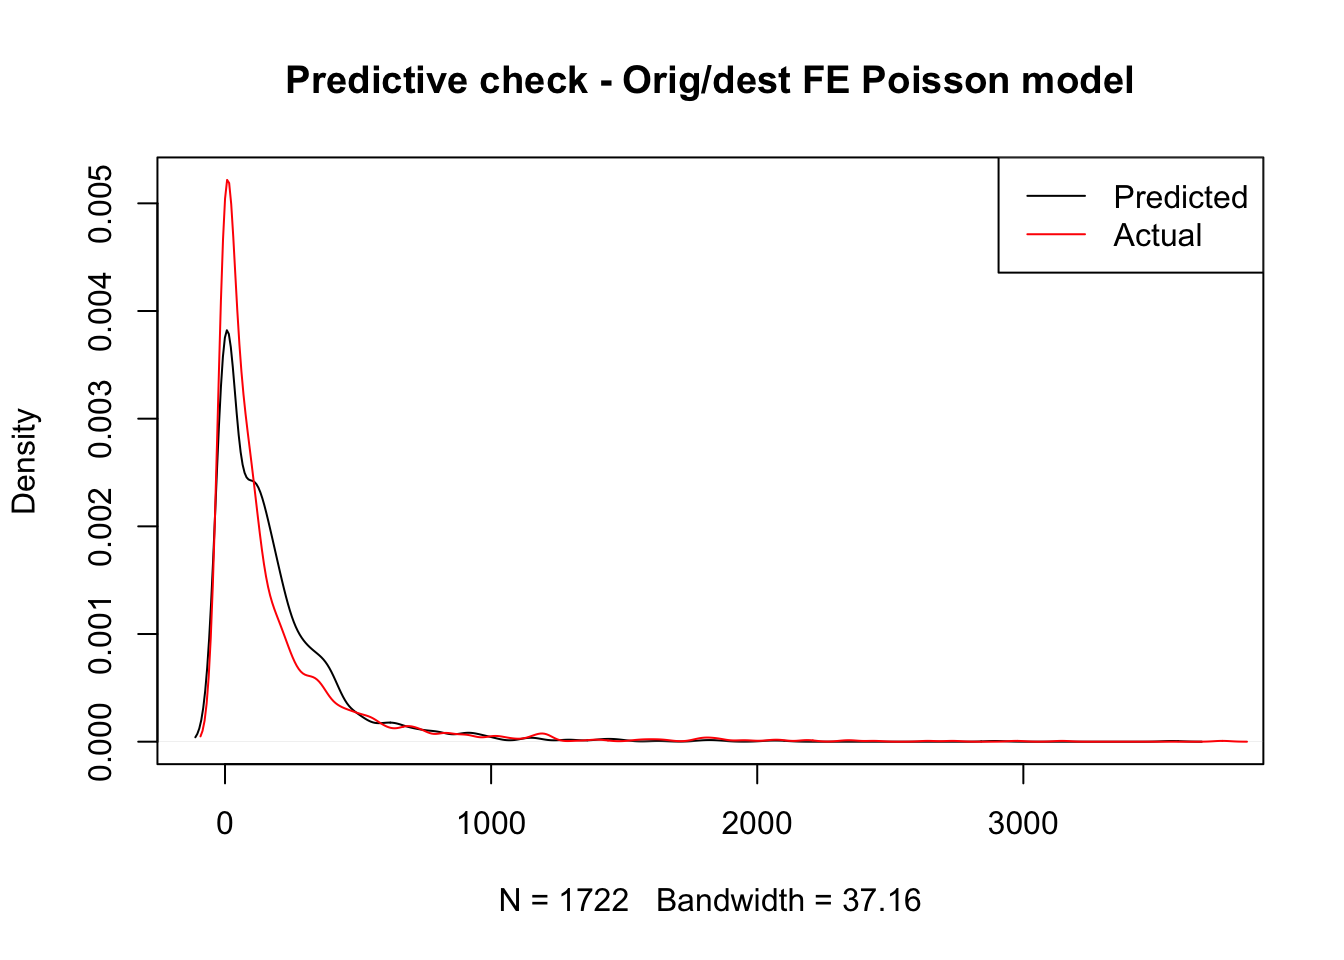
\includegraphics{05-flows_files/figure-pdf/unnamed-chunk-26-1.pdf}

Hard to tell any noticeable difference, right? To see if there is any,
we can have a look at the estimates obtained:

\begin{Shaded}
\begin{Highlighting}[]
\FunctionTok{summary}\NormalTok{(m4)}\SpecialCharTok{$}\NormalTok{coefficients[}\StringTok{\textquotesingle{}street\_dist\textquotesingle{}}\NormalTok{, ]}
\end{Highlighting}
\end{Shaded}

\begin{verbatim}
      Estimate     Std. Error        z value       Pr(>|z|) 
 -9.961619e-02   2.688731e-03  -3.704952e+01  1.828096e-300 
\end{verbatim}

And compare this to that of the straight distances in the previous
model:

\begin{Shaded}
\begin{Highlighting}[]
\FunctionTok{summary}\NormalTok{(m3)}\SpecialCharTok{$}\NormalTok{coefficients[}\StringTok{\textquotesingle{}straight\_dist\textquotesingle{}}\NormalTok{, ]}
\end{Highlighting}
\end{Shaded}

\begin{verbatim}
      Estimate     Std. Error        z value       Pr(>|z|) 
 -7.820014e-02   2.683052e-03  -2.914596e+01  9.399407e-187 
\end{verbatim}

As we can see, the differences exist but they are not massive. Let's use
this example to learn how to interpret coefficients in a Poisson
model\footnote{See section 6.2 of Gelman and Hill (2006) for a similar
  treatment of these.}. Effectively, these estimates can be understood
as multiplicative effects. Since our model fits

\[
T_{ij} \sim Poisson (\exp^{X_{ij}\beta})
\]

we need to transform \(\beta\) through an exponential in order to get a
sense of the effect of distance on the number of trips. This means that
for the street distance, our original estimate is
\(\beta_{street} = -0.0996\), but this needs to be translated through
the exponential into \(e^{-0.0996} = 0.906\). In other words, since
distance is expressed in standard deviations\footnote{Remember the
  transformation at the very beginning.}, we can expect a 10\% decrease
in the number of trips for an increase of one standard deviation (about
1Km) in the distance between the stations. This can be compared with
\(e^{-0.0782} = 0.925\) for the straight distances, or a reduction of
about 8\% the number of trips for every increase of a standard deviation
(about 720m).

\section{Predicting flows}\label{predicting-flows}

So far we have put all of our modeling efforts in understanding the
model we fit and improving such model so it fits our data as closely as
possible. This is essential in any modelling exercise but should be far
from a stopping point. Once we're confident our model is a decent
representation of the data generating process, we can start exploiting
it. In this section, we will cover one specific case that showcases how
a fitted model can help: out-of-sample forecasts.

It is August 2015, and you have just started working as a data scientist
for the bikeshare company that runs the San Francisco system. You join
them as they're planning for the next academic year and, in order to
plan their operations (re-allocating vans, station maintenance, etc.),
they need to get a sense of how many people are going to be pedalling
across the city and, crucially, \emph{where} they are going to be
pedalling through. What can you do to help them?

The easiest approach is to say ``well, a good guess for how many people
will be going between two given stations this coming year is how many
went through last year, isn't it?''. This is one prediction approach.
However, you could see how, even if the same process governs over both
datasets (2015 and 2016), each year will probably have some
idiosyncracies and thus looking too closely into one year might not give
the best possible answer for the next one. Ideally, you want a good
stylized synthesis that captures the bits that stay constant over time
and thus can be applied in the future and that ignores those aspects
that are too particular to a given point in time. That is the rationale
behind using a fitted model to obtain predictions.

However good any theory though, the truth is in the pudding. So, to see
if a modeling approach is better at producing forecasts than just using
the counts from last year, we can put them to a test. The way this is
done when evaluating the predictive performance of a model (as this is
called in the literature) relies on two basic steps: a) obtain
predictions from a given model and b) compare those to the actual values
(in our case, with the counts for 2016 in \texttt{trips16}) and get a
sense of ``how off'' they are. We have essentially covered a) above; for
b), there are several measures to use. We will use one of the most
common ones, the root mean squared error (RMSE), which roughly gives a
sense of the average difference between a predicted vector and the real
deal:

\[
RMSE = \sqrt{ \sum_{ij} (\hat{T_{ij}} - T_{ij})^2}
\]

where \(\hat{T_{ij}}\) is the predicted amount of trips between stations
\(i\) and \(j\). RMSE is straightforward in R and, since we will use it
a couple of times, let's write a short function to make our lives
easier:

\begin{Shaded}
\begin{Highlighting}[]
\NormalTok{rmse }\OtherTok{\textless{}{-}} \ControlFlowTok{function}\NormalTok{(t, p)\{}
\NormalTok{  se }\OtherTok{\textless{}{-}}\NormalTok{ (t }\SpecialCharTok{{-}}\NormalTok{ p)}\SpecialCharTok{\^{}}\DecValTok{2}
\NormalTok{  mse }\OtherTok{\textless{}{-}} \FunctionTok{mean}\NormalTok{(se)}
\NormalTok{  rmse }\OtherTok{\textless{}{-}} \FunctionTok{sqrt}\NormalTok{(mse)}
  \FunctionTok{return}\NormalTok{(rmse)}
\NormalTok{\}}
\end{Highlighting}
\end{Shaded}

where \texttt{t} stands for the vector of true values, and \texttt{p} is
the vector of predictions. Let's give it a spin to make sure it works:

\begin{Shaded}
\begin{Highlighting}[]
\NormalTok{rmse\_m4 }\OtherTok{\textless{}{-}} \FunctionTok{rmse}\NormalTok{(db\_std}\SpecialCharTok{$}\NormalTok{trips16, m4}\SpecialCharTok{$}\NormalTok{fitted.values)}
\NormalTok{rmse\_m4}
\end{Highlighting}
\end{Shaded}

\begin{verbatim}
[1] 256.2197
\end{verbatim}

That means that, on average, predictions in our best model \texttt{m4}
are 256 trips off. Is this good? Bad? Worse? It's hard to say but, being
practical, what we can say is whether this better than our alternative.
Let us have a look at the RMSE of the other models as well as that of
simply plugging in last year's counts:{[}\^{}05-flows-11{]}

\marginnote{\begin{footnotesize}

\begin{tcolorbox}[enhanced jigsaw, colframe=quarto-callout-tip-color-frame, leftrule=.75mm, arc=.35mm, breakable, opacityback=0, bottomrule=.15mm, colback=white, rightrule=.15mm, toprule=.15mm, left=2mm]

\textbf{Task}

Can you create a single plot that displays the distribution of the
predicted values of the five different ways to predict trips in 2016 and
the actual counts of trips?

\end{tcolorbox}

\end{footnotesize}}

\begin{Shaded}
\begin{Highlighting}[]
\NormalTok{rmses }\OtherTok{\textless{}{-}} \FunctionTok{data.frame}\NormalTok{(}
  \AttributeTok{model=}\FunctionTok{c}\NormalTok{(}
    \StringTok{\textquotesingle{}OLS\textquotesingle{}}\NormalTok{, }
    \StringTok{\textquotesingle{}Poisson\textquotesingle{}}\NormalTok{, }
    \StringTok{\textquotesingle{}Poisson + FE\textquotesingle{}}\NormalTok{, }
    \StringTok{\textquotesingle{}Poisson + FE + street dist.\textquotesingle{}}\NormalTok{,}
    \StringTok{\textquotesingle{}Trips{-}2015\textquotesingle{}}
\NormalTok{  ),}
  \AttributeTok{RMSE=}\FunctionTok{c}\NormalTok{(}
  \FunctionTok{rmse}\NormalTok{(db\_std}\SpecialCharTok{$}\NormalTok{trips16, m1}\SpecialCharTok{$}\NormalTok{fitted.values),}
  \FunctionTok{rmse}\NormalTok{(db\_std}\SpecialCharTok{$}\NormalTok{trips16, m2}\SpecialCharTok{$}\NormalTok{fitted.values),}
  \FunctionTok{rmse}\NormalTok{(db\_std}\SpecialCharTok{$}\NormalTok{trips16, m3}\SpecialCharTok{$}\NormalTok{fitted.values),}
  \FunctionTok{rmse}\NormalTok{(db\_std}\SpecialCharTok{$}\NormalTok{trips16, m4}\SpecialCharTok{$}\NormalTok{fitted.values),}
  \FunctionTok{rmse}\NormalTok{(db\_std}\SpecialCharTok{$}\NormalTok{trips16, db\_std}\SpecialCharTok{$}\NormalTok{trips15)}
\NormalTok{  )}
\NormalTok{)}
\NormalTok{rmses}
\end{Highlighting}
\end{Shaded}

\begin{verbatim}
                        model     RMSE
1                         OLS 323.6135
2                     Poisson 320.8962
3                Poisson + FE 254.4468
4 Poisson + FE + street dist. 256.2197
5                  Trips-2015 131.0228
\end{verbatim}

The table is both encouraging and disheartning at the same time. On the
one hand, all the modeling techniques covered above behave as we would
expect: the baseline model displays the worst predicting power of all,
and every improvement (except the street distances!) results in notable
decreases of the RMSE. This is good news. However, on the other hand,
all of our modelling efforts fall short of given a better guess than
simply using the previous year's counts. \emph{Why? Does this mean that
we should not pay attention to modeling and inference?} Not really.
Generally speaking, a model is as good at predicting as it is able to
mimic the underlying process that gave rise to the data in the first
place. The results above point to a case where our model is not picking
up all the factors that determine the amount of trips undertaken in a
give route. This could be improved by enriching the model with
more/better predictors, as we have seen above. Also, the example above
seems to point to a case where those idiosyncracies in 2015 that the
model does not pick up seem to be at work in 2016 as well. This is great
news for our prediction efforts this time, but we have no idea why this
is the case and, for all that matters, it could change the coming year.
Besides the elegant quantification of uncertainty, the true advantage of
a modeling approach in this context is that, if well fit, it is able to
pick up the fundamentals that apply over and over. This means that, if
next year we're not as lucky as this one and previous counts are not
good predictors but the variables we used in our model continue to have
a role in determining the outcome, the data scientist should be luckier
and hit a better prediction.

\section{Questions}\label{questions-1}

We will be using again the Madrid AirBnb dataset:

\begin{Shaded}
\begin{Highlighting}[]
\NormalTok{mad\_abb }\OtherTok{\textless{}{-}} \FunctionTok{st\_read}\NormalTok{(}\StringTok{\textquotesingle{}./data/assignment\_1\_madrid/madrid\_abb.gpkg\textquotesingle{}}\NormalTok{)}
\end{Highlighting}
\end{Shaded}

\begin{verbatim}
Reading layer `madrid_abb' from data source 
  `/Users/franciscorowe/Dropbox/Francisco/uol/teaching/envs453/202324/san/data/assignment_1_madrid/madrid_abb.gpkg' 
  using driver `GPKG'
Simple feature collection with 18399 features and 16 fields
Geometry type: POINT
Dimension:     XY
Bounding box:  xmin: -3.86391 ymin: 40.33243 xmax: -3.556 ymax: 40.56274
Geodetic CRS:  WGS 84
\end{verbatim}

The columns to use here are:

\begin{itemize}
\tightlist
\item
  \texttt{price\_usd}: price expressed in USD
\item
  \texttt{log1p\_price\_usd}: logarithm of the price expressed in USD
\item
  \texttt{accommodates}: number of people the property accommodates
\item
  \texttt{bathrooms}: number of bathrooms the property includes
\item
  \texttt{bedrooms}: number of bedrooms the property includes
\item
  \texttt{beds}: number of beds the property includes
\end{itemize}

With these data at hand, accomplish the following challenges:

\begin{enumerate}
\def\labelenumi{\arabic{enumi}.}
\tightlist
\item
  Set up a baseline regression model where you explain the price of a
  property as a function of its characteristics:
\end{enumerate}

\[
P_i = \alpha + \beta_1 Acc_i + \beta_2 Bath_i + \beta_3 Bedr_i + \beta_4 Beds_i + \epsilon_i
\]

\begin{enumerate}
\def\labelenumi{\arabic{enumi}.}
\setcounter{enumi}{1}
\tightlist
\item
  Fit a parallel model that uses the log of price as dependent variable:
\end{enumerate}

\[
\log(P_i) = \alpha + \beta_1 Acc_i + \beta_2 Bath_i + \beta_3 Bedr_i + \beta_4 Beds_i + \epsilon_i
\]

\begin{enumerate}
\def\labelenumi{\arabic{enumi}.}
\setcounter{enumi}{2}
\tightlist
\item
  Perform a predictive check analysis of both models, discussing how
  they compare, which one you would prefer, and why
\end{enumerate}

\bookmarksetup{startatroot}

\chapter{Spatial Econometrics}\label{sec-chp6}

This chapter is based on the following references, which are good
follow-up's on the topic:

\begin{itemize}
\tightlist
\item
  \href{https://geographicdata.science/book/notebooks/11_regression.html}{Chapter
  11} of the GDS Book, by Rey, Arribas-Bel, and Wolf (2023).
\item
  \href{http://darribas.org/sdar_mini/notes/Class_03.html}{Session III}
  of Dani Arribas-Bel (2014). Check the ``Related readings'' section on
  the session page for more in-depth discussions.
\item
  Anselin (2007), freely available to download
  {[}\href{https://dces.wisc.edu/wp-content/uploads/sites/128/2013/08/W14_Anselin2007.pdf}{\texttt{pdf}}{]}.
\item
  The second part of this tutorial assumes you have reviewed
  \href{https://darribas.org/gds_course/content/bE/concepts_E.html}{the
  Spatial Weights Section} of Dani Arribas-Bel (2019).
\end{itemize}

\section{Dependencies}\label{dependencies-3}

We will rely on the following libraries in this section, all of them
included in Section~\ref{sec-dependencies}:

\begin{Shaded}
\begin{Highlighting}[]
\CommentTok{\# Data management}
\FunctionTok{library}\NormalTok{(tidyverse)}
\CommentTok{\# Spatial Data management}
\FunctionTok{library}\NormalTok{(sf)}
\CommentTok{\# For all your interpolation needs}
\FunctionTok{library}\NormalTok{(gstat)}
\CommentTok{\# Spatial regression}
\FunctionTok{library}\NormalTok{(spdep)}
\end{Highlighting}
\end{Shaded}

\section{Data}\label{data-2}

To explore ideas in spatial regression, we will the set of Airbnb
properties for San Diego (US), borrowed from the ``Geographic Data
Science with Python'' book (see
\href{https://geographicdata.science/book/data/airbnb/regression_cleaning.html}{here}
for more info on the dataset source). This covers the point location of
properties advertised on the Airbnb website in the San Diego region.

Let us load the data:

\begin{Shaded}
\begin{Highlighting}[]
\NormalTok{db }\OtherTok{\textless{}{-}} \FunctionTok{st\_read}\NormalTok{(}\StringTok{\textquotesingle{}data/abb\_sd/regression\_db.geojson\textquotesingle{}}\NormalTok{)}
\end{Highlighting}
\end{Shaded}

\begin{verbatim}
Reading layer `regression_db' from data source 
  `/Users/franciscorowe/Dropbox/Francisco/uol/teaching/envs453/202324/san/data/abb_sd/regression_db.geojson' 
  using driver `GeoJSON'
Simple feature collection with 6110 features and 19 fields
Geometry type: POINT
Dimension:     XY
Bounding box:  xmin: -117.2812 ymin: 32.57349 xmax: -116.9553 ymax: 33.08311
Geodetic CRS:  WGS 84
\end{verbatim}

The table contains the followig variables:

\begin{Shaded}
\begin{Highlighting}[]
\FunctionTok{names}\NormalTok{(db)}
\end{Highlighting}
\end{Shaded}

\begin{verbatim}
 [1] "accommodates"       "bathrooms"          "bedrooms"          
 [4] "beds"               "neighborhood"       "pool"              
 [7] "d2balboa"           "coastal"            "price"             
[10] "log_price"          "id"                 "pg_Apartment"      
[13] "pg_Condominium"     "pg_House"           "pg_Other"          
[16] "pg_Townhouse"       "rt_Entire_home.apt" "rt_Private_room"   
[19] "rt_Shared_room"     "geometry"          
\end{verbatim}

For most of this chapter, we will be exploring determinants and
strategies for modelling the price of a property advertised in AirBnb.
To get a first taste of what this means, we can create a plot of prices
within the area of San Diego:

\begin{Shaded}
\begin{Highlighting}[]
\NormalTok{db }\SpecialCharTok{\%\textgreater{}\%}
  \FunctionTok{ggplot}\NormalTok{(}\FunctionTok{aes}\NormalTok{(}\AttributeTok{color =}\NormalTok{ price)) }\SpecialCharTok{+}
  \FunctionTok{geom\_sf}\NormalTok{() }\SpecialCharTok{+} 
  \FunctionTok{scale\_color\_viridis\_c}\NormalTok{() }\SpecialCharTok{+}
  \FunctionTok{theme\_void}\NormalTok{()}
\end{Highlighting}
\end{Shaded}

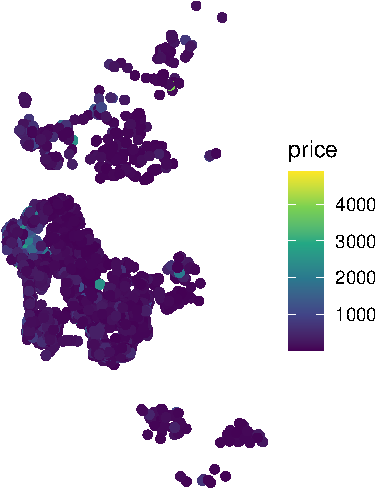
\includegraphics{06-spatial-econometrics_files/figure-pdf/unnamed-chunk-4-1.pdf}

\section{Non-spatial regression, a
refresh}\label{non-spatial-regression-a-refresh}

Before we discuss how to explicitly include space into the linear
regression framework, let us show how basic regression can be carried
out in R, and how you can interpret the results. By no means is this a
formal and complete introduction to regression so, if that is what you
are looking for, the first part of Gelman and Hill (2006), in particular
chapters 3 and 4, are excellent places to check out.

The core idea of linear regression is to explain the variation in a
given (\emph{dependent}) variable as a linear function of a series of
other (\emph{explanatory}) variables. For example, in our case, we may
want to express/explain the price of a property advertised on AirBnb as
a function of some of its characteristics, such as the number of people
it accommodates, and how many bathrooms, bedrooms and beds it features.
At the individual level, we can express this as:

\[
\log(P_i) = \alpha + \beta_1 Acc_i + \beta_2 Bath_i + \beta_3 Bedr_i + \beta_4 Beds_i + \epsilon_i
\]

where \(P_i\) is the price of house \(i\), \(Acc_i\), \(Bath_i\),
\(Bedr_i\) and \(Beds_i\) are the count of people it accommodates,
bathrooms, bedrooms and beds that house \(i\) has, respectively. The
parameters \(\beta_{1,2, 3, 4}\) give us information about in which way
and to what extent each variable is related to the price, and
\(\alpha\), the constant term, is the average house price when all the
other variables are zero. The term \(\epsilon_i\) is usually referred to
as the ``error'' and captures elements that influence the price of a
house but are not accounted for explicitly. We can also express this
relation in matrix form, excluding subindices for \(i\) as:

\[
\log(P) = \alpha + \beta_1 Acc + \beta_2 Bath + \beta_3 Bedr + \beta_4 Beds + \epsilon
\] where each term can be interpreted in terms of vectors instead of
scalars (wit the exception of the parameters
\((\alpha, \beta_{1, 2, 3, 4})\), which \emph{are} scalars). Note we are
using the logarithm of the price, since this allows us to interpret the
coefficients as roughly the percentage change induced by a unit increase
in the explanatory variable of the estimate.

Remember a regression can be seen as a multivariate extension of
bivariate correlations. Indeed, one way to interpret the \(\beta_k\)
coefficients in the equation above is as the degree of correlation
between the explanatory variable \(k\) and the dependent variable,
\emph{keeping all the other explanatory variables constant}. When you
calculate simple bivariate correlations, the coefficient of a variable
is picking up the correlation between the variables, but it is also
subsuming into it variation associated with other correlated variables
--also called confounding factors{[}\^{}06-spatial-econometrics-1{]}.
Regression allows you to isolate the distinct effect that a single
variable has on the dependent one, once we \emph{control} for those
other variables.

\marginnote{\begin{footnotesize}

\begin{tcolorbox}[enhanced jigsaw, colframe=quarto-callout-tip-color-frame, leftrule=.75mm, arc=.35mm, breakable, opacityback=0, bottomrule=.15mm, colback=white, rightrule=.15mm, toprule=.15mm, left=2mm]

\textbf{Task}

Assume that new houses tend to be built more often in areas with low
deprivation. If that is the case, then \(NEW\) and \(IMD\) will be
correlated with each other (as well as with the price of a house, as we
are hypothesizing in this case). If we calculate a simple correlation
between \(P\) and \(IMD\), the coefficient will represent the degree of
association between both variables, but it will also include some of the
association between \(IMD\) and \(NEW\). That is, part of the obtained
correlation coefficient will be due not to the fact that higher prices
tend to be found in areas with low IMD, but to the fact that new houses
tend to be more expensive. This is because (in this example) new houses
tend to be built in areas with low deprivation and simple bivariate
correlation cannot account for that.

\end{tcolorbox}

\end{footnotesize}}

Practically speaking, running linear regressions in \texttt{R} is
straightforward. For example, to fit the model specified in the equation
above, we only need one line of code:

\begin{Shaded}
\begin{Highlighting}[]
\NormalTok{m1 }\OtherTok{\textless{}{-}} \FunctionTok{lm}\NormalTok{(}\StringTok{\textquotesingle{}log\_price \textasciitilde{} accommodates + bathrooms + bedrooms + beds\textquotesingle{}}\NormalTok{, db)}
\end{Highlighting}
\end{Shaded}

We use the command \texttt{lm}, for linear model, and specify the
equation we want to fit using a string that relates the dependent
variable (the log of the price, \texttt{log\_price}) with a set of
explanatory ones (\texttt{accommodates}, \texttt{bathrooms},
\texttt{bedrooms}, \texttt{beds}) by using a tilde
\texttt{\textasciitilde{}} that is akin to the \(=\) symbol in the
mathematical equation above. Since we are using names of variables that
are stored in a table, we need to pass the table object (\texttt{db}) as
well.

In order to inspect the results of the model, the quickest way is to
call \texttt{summary}:

\begin{Shaded}
\begin{Highlighting}[]
\FunctionTok{summary}\NormalTok{(m1)}
\end{Highlighting}
\end{Shaded}

\begin{verbatim}

Call:
lm(formula = "log_price ~ accommodates + bathrooms + bedrooms + beds", 
    data = db)

Residuals:
    Min      1Q  Median      3Q     Max 
-2.8486 -0.3234 -0.0095  0.3023  3.3975 

Coefficients:
              Estimate Std. Error t value Pr(>|t|)    
(Intercept)   4.018133   0.013947  288.10   <2e-16 ***
accommodates  0.176851   0.005323   33.23   <2e-16 ***
bathrooms     0.150981   0.012526   12.05   <2e-16 ***
bedrooms      0.111700   0.012537    8.91   <2e-16 ***
beds         -0.076974   0.007927   -9.71   <2e-16 ***
---
Signif. codes:  0 '***' 0.001 '**' 0.01 '*' 0.05 '.' 0.1 ' ' 1

Residual standard error: 0.5366 on 6105 degrees of freedom
Multiple R-squared:  0.5583,    Adjusted R-squared:  0.558 
F-statistic:  1929 on 4 and 6105 DF,  p-value: < 2.2e-16
\end{verbatim}

A full detailed explanation of the output is beyond the scope of the
chapter, but we will highlight the relevant bits for our main purpose.
This is concentrated on the \texttt{Coefficients} section, which gives
us the estimates for the \(\beta_k\) coefficients in our model. These
estimates are the raw equivalent of the correlation coefficient between
each explanatory variable and the dependent one, once the ``polluting''
effect of the other variables included in the model has been accounted
for\footnote{Keep in mind that regression is no magic. We are only
  discounting the effect of other confounding factors that we include in
  the model, not of \emph{all} potentially confounding factors.}.
Results are as expected for the most part: houses tend to be
significantly more expensive if they accommodate more people (an extra
person increases the price by 17.7\%, approximately), have more
bathrooms (15.1\%), or bedrooms (11.2\%). Perhaps counter intuitively,
an extra bed available seems to decrease the price by about -7.7\%.
However, keep in mind that this is the case, \emph{everything else
equal}. Hence, more beds per room and bathroom (ie. a more crowded
house) is a bit cheaper.

\section{Spatial regression: a (very) first
dip}\label{spatial-regression-a-very-first-dip}

Spatial regression is about \emph{explicitly} introducing space or
geographical context into the statistical framework of a regression.
Conceptually, we want to introduce space into our model whenever we
think it plays an important role in the process we are interested in, or
when space can act as a reasonable proxy for other factors we cannot but
should include in our model. As an example of the former, we can imagine
how houses at the seafront are probably more expensive than those in the
second row, given their better views. To illustrate the latter, we can
think of how the character of a neighborhood is important in determining
the price of a house; however, it is very hard to identify and quantify
``character'' per se, although it might be easier to get at its spatial
variation, hence a case of space as a proxy.

Spatial regression is a large field of development in the econometrics
and statistics literature. In this brief introduction, we will consider
two related but very different processes that give rise to spatial
effects: spatial heterogeneity and spatial dependence. For more rigorous
treatments of the topics introduced here, the reader is referred to
Anselin (2003), Anselin and Rey (2014), and Gibbons, Overman, and
Patacchini (2014).

\section{Spatial heterogeneity}\label{spatial-heterogeneity-1}

Spatial heterogeneity (SH) arises when we cannot safely assume the
process we are studying operates under the same ``rules'' throughout the
geography of interest. In other words, we can observe SH when there are
effects on the outcome variable that are intrinsically linked to
specific locations. A good example of this is the case of seafront
houses above: we are trying to model the price of a house and, the fact
some houses are located under certain conditions (i.e.~by the sea),
makes their price behave differently. This somewhat abstract concept of
SH can be made operational in a model in several ways. We will explore
the following two: spatial fixed-effects (FE); and spatial regimes,
which is a generalization of FE.

\textbf{Spatial FE}

Let us consider the house price example from the previous section to
introduce a more general illustration that relates to the second
motivation for spatial effects (``space as a proxy''). Given we are only
including two explanatory variables in the model, it is likely we are
missing some important factors that play a role at determining the price
at which a house is sold. Some of them, however, are likely to vary
systematically over space (e.g.~different neighborhood characteristics).
If that is the case, we can control for those unobserved factors by
using traditional dummy variables but basing their creation on a spatial
rule. For example, let us include a binary variable for every
neighbourhood, as provided by AirBnB, indicating whether a given house
is located within such area (\texttt{1}) or not (\texttt{0}).
Neighbourhood membership is expressed on the \texttt{neighborhood}
column:

\begin{Shaded}
\begin{Highlighting}[]
\NormalTok{db }\SpecialCharTok{\%\textgreater{}\%}
  \FunctionTok{ggplot}\NormalTok{(}\FunctionTok{aes}\NormalTok{(}\AttributeTok{color =}\NormalTok{ neighborhood)) }\SpecialCharTok{+}
  \FunctionTok{geom\_sf}\NormalTok{() }\SpecialCharTok{+} 
  \FunctionTok{theme\_void}\NormalTok{()}
\end{Highlighting}
\end{Shaded}

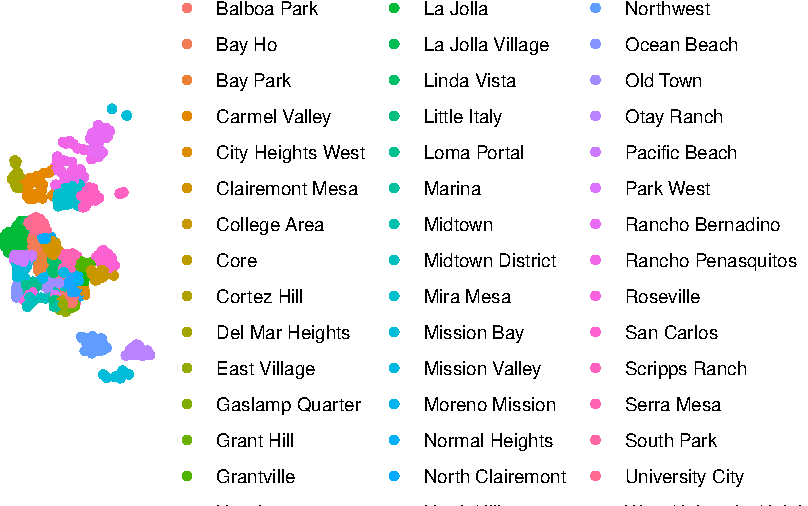
\includegraphics{06-spatial-econometrics_files/figure-pdf/unnamed-chunk-7-1.pdf}

Mathematically, we are now fitting the following equation:

\[
\log(P_i) = \alpha_r + \beta_1 Acc_i + \beta_2 Bath_i + \beta_3 Bedr_i + \beta_4 Beds_i + \epsilon_i
\]

where the main difference is that we are now allowing the constant term,
\(\alpha\), to vary by neighbourhood \(r\), \(\alpha_r\).

Programmatically, we can fit this model with \texttt{lm}:

\begin{Shaded}
\begin{Highlighting}[]
\CommentTok{\# Include \textasciigrave{}{-}1\textasciigrave{} to eliminate the constant term and include a dummy for every area}
\NormalTok{m2 }\OtherTok{\textless{}{-}} \FunctionTok{lm}\NormalTok{(}
  \StringTok{\textquotesingle{}log\_price \textasciitilde{} neighborhood + accommodates + bathrooms + bedrooms + beds {-} 1\textquotesingle{}}\NormalTok{, }
\NormalTok{  db}
\NormalTok{)}
\FunctionTok{summary}\NormalTok{(m2)}
\end{Highlighting}
\end{Shaded}

\begin{verbatim}

Call:
lm(formula = "log_price ~ neighborhood + accommodates + bathrooms + bedrooms + beds - 1", 
    data = db)

Residuals:
    Min      1Q  Median      3Q     Max 
-2.4549 -0.2920 -0.0203  0.2741  3.5323 

Coefficients:
                                     Estimate Std. Error t value Pr(>|t|)    
neighborhoodBalboa Park              3.994775   0.036539  109.33   <2e-16 ***
neighborhoodBay Ho                   3.780025   0.086081   43.91   <2e-16 ***
neighborhoodBay Park                 3.941847   0.055788   70.66   <2e-16 ***
neighborhoodCarmel Valley            4.034052   0.062811   64.23   <2e-16 ***
neighborhoodCity Heights West        3.698788   0.065502   56.47   <2e-16 ***
neighborhoodClairemont Mesa          3.658339   0.051438   71.12   <2e-16 ***
neighborhoodCollege Area             3.649859   0.064979   56.17   <2e-16 ***
neighborhoodCore                     4.433447   0.058864   75.32   <2e-16 ***
neighborhoodCortez Hill              4.294790   0.057648   74.50   <2e-16 ***
neighborhoodDel Mar Heights          4.300659   0.060912   70.61   <2e-16 ***
neighborhoodEast Village             4.241146   0.032019  132.46   <2e-16 ***
neighborhoodGaslamp Quarter          4.473863   0.052493   85.23   <2e-16 ***
neighborhoodGrant Hill               4.001481   0.058825   68.02   <2e-16 ***
neighborhoodGrantville               3.664989   0.080168   45.72   <2e-16 ***
neighborhoodKensington               4.073520   0.087322   46.65   <2e-16 ***
neighborhoodLa Jolla                 4.400145   0.026772  164.36   <2e-16 ***
neighborhoodLa Jolla Village         4.066151   0.087263   46.60   <2e-16 ***
neighborhoodLinda Vista              3.817940   0.063128   60.48   <2e-16 ***
neighborhoodLittle Italy             4.390651   0.052433   83.74   <2e-16 ***
neighborhoodLoma Portal              4.034473   0.036173  111.53   <2e-16 ***
neighborhoodMarina                   4.046133   0.052178   77.55   <2e-16 ***
neighborhoodMidtown                  4.032038   0.030280  133.16   <2e-16 ***
neighborhoodMidtown District         4.356943   0.071756   60.72   <2e-16 ***
neighborhoodMira Mesa                3.570523   0.061543   58.02   <2e-16 ***
neighborhoodMission Bay              4.251309   0.023318  182.32   <2e-16 ***
neighborhoodMission Valley           4.012410   0.083766   47.90   <2e-16 ***
neighborhoodMoreno Mission           4.028288   0.063342   63.59   <2e-16 ***
neighborhoodNormal Heights           3.791895   0.054730   69.28   <2e-16 ***
neighborhoodNorth Clairemont         3.498107   0.076432   45.77   <2e-16 ***
neighborhoodNorth Hills              3.959403   0.026823  147.61   <2e-16 ***
neighborhoodNorthwest                3.810201   0.078158   48.75   <2e-16 ***
neighborhoodOcean Beach              4.152695   0.032352  128.36   <2e-16 ***
neighborhoodOld Town                 4.127737   0.046523   88.72   <2e-16 ***
neighborhoodOtay Ranch               3.722902   0.091633   40.63   <2e-16 ***
neighborhoodPacific Beach            4.116749   0.022711  181.27   <2e-16 ***
neighborhoodPark West                4.216829   0.050370   83.72   <2e-16 ***
neighborhoodRancho Bernadino         3.873962   0.080780   47.96   <2e-16 ***
neighborhoodRancho Penasquitos       3.772037   0.068808   54.82   <2e-16 ***
neighborhoodRoseville                4.070468   0.065299   62.34   <2e-16 ***
neighborhoodSan Carlos               3.935042   0.093205   42.22   <2e-16 ***
neighborhoodScripps Ranch            3.641239   0.085190   42.74   <2e-16 ***
neighborhoodSerra Mesa               3.912127   0.066630   58.71   <2e-16 ***
neighborhoodSouth Park               3.987019   0.060141   66.30   <2e-16 ***
neighborhoodUniversity City          3.772504   0.039638   95.17   <2e-16 ***
neighborhoodWest University Heights  4.043161   0.048238   83.82   <2e-16 ***
accommodates                         0.150283   0.005086   29.55   <2e-16 ***
bathrooms                            0.132287   0.011886   11.13   <2e-16 ***
bedrooms                             0.147631   0.011960   12.34   <2e-16 ***
beds                                -0.074622   0.007405  -10.08   <2e-16 ***
---
Signif. codes:  0 '***' 0.001 '**' 0.01 '*' 0.05 '.' 0.1 ' ' 1

Residual standard error: 0.4971 on 6061 degrees of freedom
Multiple R-squared:  0.9904,    Adjusted R-squared:  0.9904 
F-statistic: 1.28e+04 on 49 and 6061 DF,  p-value: < 2.2e-16
\end{verbatim}

Econometrically speaking, what the postcode FE we have introduced imply
is that, instead of comparing all house prices across San Diego as
equal, we only derive variation from \emph{within} each postcode. In our
particular case, estimating spatial FE in our particular example also
gives you an indirect measure of area \emph{desirability}: since they
are simple dummies in a regression explaining the price of a house,
their estimate tells us about how much people are willing to pay to live
in a given area. We can visualise this ``geography of desirability'' by
plotting the estimates of each fixed effect on a map:

\begin{Shaded}
\begin{Highlighting}[]
\CommentTok{\# Extract neighborhood names from coefficients}
\NormalTok{nei.names }\OtherTok{\textless{}{-}}\NormalTok{ m2}\SpecialCharTok{$}\NormalTok{coefficients }\SpecialCharTok{\%\textgreater{}\%}
  \FunctionTok{as.data.frame}\NormalTok{() }\SpecialCharTok{\%\textgreater{}\%}
  \FunctionTok{row.names}\NormalTok{() }\SpecialCharTok{\%\textgreater{}\%}
  \FunctionTok{str\_replace}\NormalTok{(}\StringTok{"neighborhood"}\NormalTok{, }\StringTok{""}\NormalTok{)}
\CommentTok{\# Set up as Data Frame}
\NormalTok{nei.fes }\OtherTok{\textless{}{-}} \FunctionTok{data.frame}\NormalTok{(}
  \AttributeTok{coef =}\NormalTok{ m2}\SpecialCharTok{$}\NormalTok{coefficients,}
  \AttributeTok{nei =}\NormalTok{ nei.names,}
  \AttributeTok{row.names =}\NormalTok{ nei.names}
\NormalTok{) }\SpecialCharTok{\%\textgreater{}\%}
  \FunctionTok{right\_join}\NormalTok{(}
\NormalTok{    db, }\AttributeTok{by =} \FunctionTok{c}\NormalTok{(}\StringTok{"nei"} \OtherTok{=} \StringTok{"neighborhood"}\NormalTok{)}
\NormalTok{)}
\CommentTok{\# Plot}
\NormalTok{nei.fes }\SpecialCharTok{\%\textgreater{}\%}
  \FunctionTok{st\_as\_sf}\NormalTok{() }\SpecialCharTok{\%\textgreater{}\%}
  \FunctionTok{ggplot}\NormalTok{(}\FunctionTok{aes}\NormalTok{(}\AttributeTok{color =}\NormalTok{ coef)) }\SpecialCharTok{+}
  \FunctionTok{geom\_sf}\NormalTok{() }\SpecialCharTok{+}
  \FunctionTok{scale\_color\_viridis\_c}\NormalTok{() }\SpecialCharTok{+}
  \FunctionTok{theme\_void}\NormalTok{()}
\end{Highlighting}
\end{Shaded}

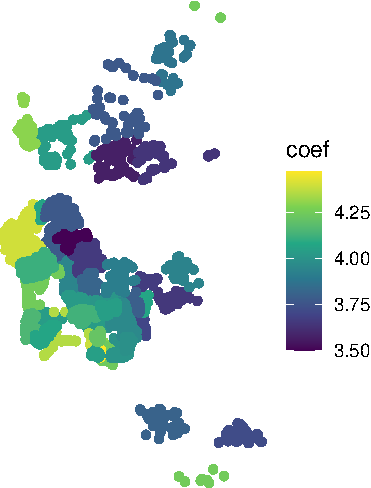
\includegraphics{06-spatial-econometrics_files/figure-pdf/unnamed-chunk-9-1.pdf}

We can see how neighborhoods in the left (west) tend to have higher
prices. What we can't see, but it is represented there if you are
familiar with the geography of San Diego, is that the city is bounded by
the Pacific ocean on the left, suggesting neighbourhoods by the beach
tend to be more expensive.

Remember that the interpretation of a \(\beta_k\) coefficient is the
effect of variable \(k\), \emph{given all the other explanatory
variables included remain constant}. By including a single variable for
each area, we are effectively forcing the model to compare as equal only
house prices that share the same value for each variable; in other
words, only houses located within the same area. Introducing FE affords
you a higher degree of isolation of the effects of the variables you
introduce in your model because you can control for unobserved effects
that align spatially with the distribution of the FE you introduce (by
neighbourhood, in our case).

\textbf{Spatial regimes}

At the core of estimating spatial FEs is the idea that, instead of
assuming the dependent variable behaves uniformly over space, there are
systematic effects following a geographical pattern that affect its
behaviour. In other words, spatial FEs introduce econometrically the
notion of spatial heterogeneity. They do this in the simplest possible
form: by allowing the constant term to vary geographically. The other
elements of the regression are left untouched and hence apply uniformly
across space. The idea of spatial regimes (SRs) is to generalize the
spatial FE approach to allow not only the constant term to vary but also
any other explanatory variable. This implies that the equation we will
be estimating is:
\[\log(P_i) = \alpha_r + \beta_{1r} Acc_i + \beta_{2r} Bath_i + \beta_{3r} Bedr_i + \beta_{4r} Beds_i + \epsilon_i\]

where we are not only allowing the constant term to vary by region
(\(\alpha_r\)), but also every other parameter (\(\beta_{kr}\)).

Also, given we are going to allow \emph{every} coefficient to vary by
regime, we will need to explicitly set a constant term that we can allow
to vary:

\begin{Shaded}
\begin{Highlighting}[]
\NormalTok{db}\SpecialCharTok{$}\NormalTok{one }\OtherTok{\textless{}{-}} \DecValTok{1}
\end{Highlighting}
\end{Shaded}

Then, the estimation leverages the capabilities in model description of
R formulas:

\begin{Shaded}
\begin{Highlighting}[]
\CommentTok{\# \textasciigrave{}:\textasciigrave{} notation implies interaction variables}
\NormalTok{m3 }\OtherTok{\textless{}{-}} \FunctionTok{lm}\NormalTok{(}
  \StringTok{\textquotesingle{}log\_price \textasciitilde{} (one + accommodates + bathrooms + bedrooms + beds):(neighborhood)\textquotesingle{}}\NormalTok{, }
\NormalTok{  db}
\NormalTok{)}
\FunctionTok{summary}\NormalTok{(m3)}
\end{Highlighting}
\end{Shaded}

\begin{verbatim}

Call:
lm(formula = "log_price ~ (one + accommodates + bathrooms + bedrooms + beds):(neighborhood)", 
    data = db)

Residuals:
    Min      1Q  Median      3Q     Max 
-2.5528 -0.2921 -0.0163  0.2586  3.1874 

Coefficients: (1 not defined because of singularities)
                                                  Estimate Std. Error t value
(Intercept)                                       4.012160   0.122261  32.816
one:neighborhoodBalboa Park                       0.128350   0.145826   0.880
one:neighborhoodBay Ho                           -0.202575   0.254393  -0.796
one:neighborhoodBay Park                         -0.272843   0.174512  -1.563
one:neighborhoodCarmel Valley                    -0.063356   0.164404  -0.385
one:neighborhoodCity Heights West                -0.096400   0.205758  -0.469
one:neighborhoodClairemont Mesa                  -0.639595   0.183891  -3.478
one:neighborhoodCollege Area                     -0.185039   0.207335  -0.892
one:neighborhoodCore                              0.416563   0.223962   1.860
one:neighborhoodCortez Hill                       0.309752   0.193169   1.604
one:neighborhoodDel Mar Heights                   0.259677   0.182046   1.426
one:neighborhoodEast Village                      0.205331   0.147158   1.395
one:neighborhoodGaslamp Quarter                  -1.156797   0.282853  -4.090
one:neighborhoodGrant Hill                       -0.077324   0.200580  -0.386
one:neighborhoodGrantville                       -0.355260   0.278718  -1.275
one:neighborhoodKensington                       -0.252743   0.248147  -1.019
one:neighborhoodLa Jolla                          0.380059   0.128014   2.969
one:neighborhoodLa Jolla Village                  0.027119   0.291318   0.093
one:neighborhoodLinda Vista                      -0.448116   0.202151  -2.217
one:neighborhoodLittle Italy                      0.384100   0.188630   2.036
one:neighborhoodLoma Portal                       0.014552   0.148157   0.098
one:neighborhoodMarina                           -0.549055   0.198350  -2.768
one:neighborhoodMidtown                           0.071392   0.134620   0.530
one:neighborhoodMidtown District                 -0.180003   0.219627  -0.820
one:neighborhoodMira Mesa                        -0.596573   0.205262  -2.906
one:neighborhoodMission Bay                       0.399054   0.128693   3.101
one:neighborhoodMission Valley                   -0.249279   0.288450  -0.864
one:neighborhoodMoreno Mission                    0.268901   0.222999   1.206
one:neighborhoodNormal Heights                   -0.253917   0.210697  -1.205
one:neighborhoodNorth Clairemont                 -0.404436   0.221559  -1.825
one:neighborhoodNorth Hills                      -0.103473   0.136994  -0.755
one:neighborhoodNorthwest                         0.198074   0.284402   0.696
one:neighborhoodOcean Beach                       0.192554   0.136493   1.411
one:neighborhoodOld Town                         -0.062746   0.157153  -0.399
one:neighborhoodOtay Ranch                       -0.358005   0.232826  -1.538
one:neighborhoodPacific Beach                     0.113854   0.129413   0.880
one:neighborhoodPark West                         0.154992   0.170398   0.910
one:neighborhoodRancho Bernadino                 -0.019347   0.194468  -0.099
one:neighborhoodRancho Penasquitos               -0.401257   0.163315  -2.457
one:neighborhoodRoseville                         0.120010   0.182676   0.657
one:neighborhoodSan Carlos                       -0.589123   0.284463  -2.071
one:neighborhoodScripps Ranch                    -0.026842   0.215965  -0.124
one:neighborhoodSerra Mesa                       -0.283949   0.207741  -1.367
one:neighborhoodSouth Park                       -0.181786   0.226828  -0.801
one:neighborhoodUniversity City                  -0.298526   0.161655  -1.847
one:neighborhoodWest University Heights                 NA         NA      NA
accommodates:neighborhoodBalboa Park              0.097052   0.024632   3.940
accommodates:neighborhoodBay Ho                  -0.017961   0.089598  -0.200
accommodates:neighborhoodBay Park                 0.155715   0.063773   2.442
accommodates:neighborhoodCarmel Valley            0.151990   0.049440   3.074
accommodates:neighborhoodCity Heights West        0.060303   0.063416   0.951
accommodates:neighborhoodClairemont Mesa          0.260414   0.050425   5.164
accommodates:neighborhoodCollege Area             0.084693   0.053125   1.594
accommodates:neighborhoodCore                     0.106661   0.039204   2.721
accommodates:neighborhoodCortez Hill              0.217358   0.037615   5.779
accommodates:neighborhoodDel Mar Heights          0.075776   0.061335   1.235
accommodates:neighborhoodEast Village             0.162155   0.020465   7.924
accommodates:neighborhoodGaslamp Quarter          0.307007   0.053766   5.710
accommodates:neighborhoodGrant Hill               0.278114   0.056238   4.945
accommodates:neighborhoodGrantville               0.124025   0.075028   1.653
accommodates:neighborhoodKensington               0.063298   0.123887   0.511
accommodates:neighborhoodLa Jolla                 0.119142   0.015162   7.858
accommodates:neighborhoodLa Jolla Village         0.207085   0.111627   1.855
accommodates:neighborhoodLinda Vista              0.172101   0.076208   2.258
accommodates:neighborhoodLittle Italy             0.230108   0.034432   6.683
accommodates:neighborhoodLoma Portal              0.090991   0.034762   2.618
accommodates:neighborhoodMarina                   0.552162   0.045914  12.026
accommodates:neighborhoodMidtown                  0.227617   0.023854   9.542
accommodates:neighborhoodMidtown District         0.179989   0.052007   3.461
accommodates:neighborhoodMira Mesa                0.157603   0.082351   1.914
accommodates:neighborhoodMission Bay              0.085754   0.013455   6.373
accommodates:neighborhoodMission Valley           0.099273   0.134176   0.740
accommodates:neighborhoodMoreno Mission           0.145824   0.060631   2.405
accommodates:neighborhoodNormal Heights           0.237177   0.053060   4.470
accommodates:neighborhoodNorth Clairemont         0.188941   0.084060   2.248
accommodates:neighborhoodNorth Hills              0.143390   0.022069   6.497
accommodates:neighborhoodNorthwest                0.022166   0.069235   0.320
accommodates:neighborhoodOcean Beach              0.113995   0.022845   4.990
accommodates:neighborhoodOld Town                 0.239088   0.042208   5.665
accommodates:neighborhoodOtay Ranch              -0.021530   0.083481  -0.258
accommodates:neighborhoodPacific Beach            0.153379   0.015339   9.999
accommodates:neighborhoodPark West                0.224593   0.045581   4.927
accommodates:neighborhoodRancho Bernadino         0.004730   0.067968   0.070
accommodates:neighborhoodRancho Penasquitos       0.070627   0.060353   1.170
accommodates:neighborhoodRoseville                0.112686   0.060090   1.875
accommodates:neighborhoodSan Carlos              -0.140714   0.087777  -1.603
accommodates:neighborhoodScripps Ranch            0.087078   0.035562   2.449
accommodates:neighborhoodSerra Mesa               0.190589   0.075803   2.514
accommodates:neighborhoodSouth Park               0.206833   0.068093   3.038
accommodates:neighborhoodUniversity City          0.067637   0.030097   2.247
accommodates:neighborhoodWest University Heights  0.124850   0.056034   2.228
bathrooms:neighborhoodBalboa Park                 0.014875   0.073585   0.202
bathrooms:neighborhoodBay Ho                      0.305028   0.225044   1.355
bathrooms:neighborhoodBay Park                    0.065043   0.120545   0.540
bathrooms:neighborhoodCarmel Valley               0.205847   0.065237   3.155
bathrooms:neighborhoodCity Heights West          -0.129465   0.183389  -0.706
bathrooms:neighborhoodClairemont Mesa             0.418033   0.176111   2.374
bathrooms:neighborhoodCollege Area               -0.012095   0.183917  -0.066
bathrooms:neighborhoodCore                        0.464974   0.186634   2.491
bathrooms:neighborhoodCortez Hill                -0.206708   0.101521  -2.036
bathrooms:neighborhoodDel Mar Heights             0.319046   0.096172   3.317
bathrooms:neighborhoodEast Village                0.312707   0.067204   4.653
bathrooms:neighborhoodGaslamp Quarter             1.459299   0.207669   7.027
bathrooms:neighborhoodGrant Hill                  0.040405   0.155867   0.259
bathrooms:neighborhoodGrantville                  0.028466   0.234973   0.121
bathrooms:neighborhoodKensington                  0.146585   0.188987   0.776
bathrooms:neighborhoodLa Jolla                    0.242760   0.026778   9.066
bathrooms:neighborhoodLa Jolla Village           -0.296748   0.326257  -0.910
bathrooms:neighborhoodLinda Vista                 0.170333   0.143441   1.187
bathrooms:neighborhoodLittle Italy                0.035532   0.111044   0.320
bathrooms:neighborhoodLoma Portal                 0.188467   0.082511   2.284
bathrooms:neighborhoodMarina                      0.316509   0.219948   1.439
bathrooms:neighborhoodMidtown                    -0.037771   0.032333  -1.168
bathrooms:neighborhoodMidtown District            0.623515   0.197674   3.154
bathrooms:neighborhoodMira Mesa                   0.215939   0.185982   1.161
bathrooms:neighborhoodMission Bay                 0.176976   0.035418   4.997
bathrooms:neighborhoodMission Valley             -0.009144   0.405637  -0.023
bathrooms:neighborhoodMoreno Mission             -0.208248   0.210241  -0.991
bathrooms:neighborhoodNormal Heights              0.017303   0.201580   0.086
bathrooms:neighborhoodNorth Clairemont           -0.102553   0.212254  -0.483
bathrooms:neighborhoodNorth Hills                 0.098449   0.064065   1.537
bathrooms:neighborhoodNorthwest                  -0.503592   0.255300  -1.973
bathrooms:neighborhoodOcean Beach                 0.082659   0.059578   1.387
bathrooms:neighborhoodOld Town                    0.087046   0.096513   0.902
bathrooms:neighborhoodOtay Ranch                 -0.219480   0.341525  -0.643
bathrooms:neighborhoodPacific Beach               0.116105   0.041006   2.831
bathrooms:neighborhoodPark West                   0.198550   0.107749   1.843
bathrooms:neighborhoodRancho Bernadino            0.365674   0.147799   2.474
bathrooms:neighborhoodRancho Penasquitos          0.320715   0.110007   2.915
bathrooms:neighborhoodRoseville                  -0.053420   0.102487  -0.521
bathrooms:neighborhoodSan Carlos                  0.267797   0.214540   1.248
bathrooms:neighborhoodScripps Ranch              -0.132692   0.169684  -0.782
bathrooms:neighborhoodSerra Mesa                  0.381620   0.197305   1.934
bathrooms:neighborhoodSouth Park                  0.087490   0.196486   0.445
bathrooms:neighborhoodUniversity City             0.138271   0.125198   1.104
bathrooms:neighborhoodWest University Heights     0.042035   0.122097   0.344
bedrooms:neighborhoodBalboa Park                  0.183347   0.065309   2.807
bedrooms:neighborhoodBay Ho                       0.241200   0.170471   1.415
bedrooms:neighborhoodBay Park                     0.214111   0.117198   1.827
bedrooms:neighborhoodCarmel Valley               -0.073928   0.127976  -0.578
bedrooms:neighborhoodCity Heights West            0.272272   0.176859   1.539
bedrooms:neighborhoodClairemont Mesa             -0.046650   0.122263  -0.382
bedrooms:neighborhoodCollege Area                -0.055707   0.108958  -0.511
bedrooms:neighborhoodCore                        -0.069929   0.108896  -0.642
bedrooms:neighborhoodCortez Hill                  0.313288   0.101770   3.078
bedrooms:neighborhoodDel Mar Heights              0.111554   0.097639   1.143
bedrooms:neighborhoodEast Village                 0.088071   0.056654   1.555
bedrooms:neighborhoodGaslamp Quarter             -0.297570   0.090336  -3.294
bedrooms:neighborhoodGrant Hill                   0.091300   0.114501   0.797
bedrooms:neighborhoodGrantville                   0.221461   0.208950   1.060
bedrooms:neighborhoodKensington                   0.450822   0.269641   1.672
bedrooms:neighborhoodLa Jolla                     0.166725   0.035423   4.707
bedrooms:neighborhoodLa Jolla Village             0.845318   0.545842   1.549
bedrooms:neighborhoodLinda Vista                  0.096413   0.171751   0.561
bedrooms:neighborhoodLittle Italy                 0.126794   0.080939   1.567
bedrooms:neighborhoodLoma Portal                  0.172480   0.067268   2.564
bedrooms:neighborhoodMarina                      -0.323085   0.137046  -2.357
bedrooms:neighborhoodMidtown                      0.172711   0.044927   3.844
bedrooms:neighborhoodMidtown District             0.088181   0.134514   0.656
bedrooms:neighborhoodMira Mesa                   -0.029149   0.206406  -0.141
bedrooms:neighborhoodMission Bay                  0.197484   0.032472   6.082
bedrooms:neighborhoodMission Valley               0.393256   0.342308   1.149
bedrooms:neighborhoodMoreno Mission              -0.081003   0.158933  -0.510
bedrooms:neighborhoodNormal Heights               0.199088   0.104514   1.905
bedrooms:neighborhoodNorth Clairemont             0.176509   0.183702   0.961
bedrooms:neighborhoodNorth Hills                  0.283826   0.047159   6.018
bedrooms:neighborhoodNorthwest                    0.411641   0.160558   2.564
bedrooms:neighborhoodOcean Beach                  0.220345   0.055039   4.003
bedrooms:neighborhoodOld Town                     0.209031   0.099966   2.091
bedrooms:neighborhoodOtay Ranch                   0.772212   0.354230   2.180
bedrooms:neighborhoodPacific Beach                0.077503   0.036735   2.110
bedrooms:neighborhoodPark West                   -0.127891   0.110497  -1.157
bedrooms:neighborhoodRancho Bernadino            -0.209594   0.160210  -1.308
bedrooms:neighborhoodRancho Penasquitos           0.107599   0.138183   0.779
bedrooms:neighborhoodRoseville                    0.395961   0.157406   2.516
bedrooms:neighborhoodSan Carlos                   0.239713   0.150420   1.594
bedrooms:neighborhoodScripps Ranch               -0.045580   0.102624  -0.444
bedrooms:neighborhoodSerra Mesa                   0.202756   0.163958   1.237
bedrooms:neighborhoodSouth Park                   0.080548   0.112861   0.714
bedrooms:neighborhoodUniversity City              0.124090   0.120386   1.031
bedrooms:neighborhoodWest University Heights      0.011105   0.095137   0.117
beds:neighborhoodBalboa Park                      0.013322   0.045740   0.291
beds:neighborhoodBay Ho                           0.037070   0.133299   0.278
beds:neighborhoodBay Park                         0.011091   0.108863   0.102
beds:neighborhoodCarmel Valley                    0.086393   0.076151   1.135
beds:neighborhoodCity Heights West                0.076520   0.132072   0.579
beds:neighborhoodClairemont Mesa                 -0.163512   0.090244  -1.812
beds:neighborhoodCollege Area                     0.228165   0.084147   2.712
beds:neighborhoodCore                            -0.080211   0.078673  -1.020
beds:neighborhoodCortez Hill                     -0.039031   0.042752  -0.913
beds:neighborhoodDel Mar Heights                 -0.021375   0.071330  -0.300
beds:neighborhoodEast Village                    -0.174883   0.040811  -4.285
beds:neighborhoodGaslamp Quarter                 -0.064063   0.088752  -0.722
beds:neighborhoodGrant Hill                      -0.178920   0.067398  -2.655
beds:neighborhoodGrantville                      -0.003795   0.126551  -0.030
beds:neighborhoodKensington                      -0.005431   0.175724  -0.031
beds:neighborhoodLa Jolla                        -0.104906   0.022470  -4.669
beds:neighborhoodLa Jolla Village                -0.385895   0.315094  -1.225
beds:neighborhoodLinda Vista                      0.032215   0.073896   0.436
beds:neighborhoodLittle Italy                    -0.145613   0.029817  -4.884
beds:neighborhoodLoma Portal                     -0.013033   0.059097  -0.221
beds:neighborhoodMarina                          -0.210771   0.113913  -1.850
beds:neighborhoodMidtown                         -0.143254   0.036531  -3.921
beds:neighborhoodMidtown District                -0.132655   0.090595  -1.464
beds:neighborhoodMira Mesa                        0.097629   0.113225   0.862
beds:neighborhoodMission Bay                     -0.061315   0.017727  -3.459
beds:neighborhoodMission Valley                   0.073187   0.235760   0.310
beds:neighborhoodMoreno Mission                   0.195918   0.116748   1.678
beds:neighborhoodNormal Heights                  -0.185827   0.062062  -2.994
beds:neighborhoodNorth Clairemont                -0.060468   0.188694  -0.320
beds:neighborhoodNorth Hills                     -0.113150   0.032768  -3.453
beds:neighborhoodNorthwest                        0.116746   0.131088   0.891
beds:neighborhoodOcean Beach                     -0.048848   0.037433  -1.305
beds:neighborhoodOld Town                        -0.158066   0.077352  -2.043
beds:neighborhoodOtay Ranch                       0.071485   0.259986   0.275
beds:neighborhoodPacific Beach                   -0.025064   0.023165  -1.082
beds:neighborhoodPark West                       -0.049627   0.063967  -0.776
beds:neighborhoodRancho Bernadino                 0.270293   0.092164   2.933
beds:neighborhoodRancho Penasquitos               0.011344   0.091156   0.124
beds:neighborhoodRoseville                       -0.085205   0.087365  -0.975
beds:neighborhoodSan Carlos                       0.550169   0.167389   3.287
beds:neighborhoodScripps Ranch                    0.219496   0.122439   1.793
beds:neighborhoodSerra Mesa                      -0.293629   0.189261  -1.551
beds:neighborhoodSouth Park                      -0.020083   0.109799  -0.183
beds:neighborhoodUniversity City                  0.124224   0.062916   1.974
beds:neighborhoodWest University Heights          0.143248   0.096150   1.490
                                                 Pr(>|t|)    
(Intercept)                                       < 2e-16 ***
one:neighborhoodBalboa Park                      0.378810    
one:neighborhoodBay Ho                           0.425887    
one:neighborhoodBay Park                         0.117997    
one:neighborhoodCarmel Valley                    0.699978    
one:neighborhoodCity Heights West                0.639437    
one:neighborhoodClairemont Mesa                  0.000509 ***
one:neighborhoodCollege Area                     0.372180    
one:neighborhoodCore                             0.062939 .  
one:neighborhoodCortez Hill                      0.108871    
one:neighborhoodDel Mar Heights                  0.153795    
one:neighborhoodEast Village                     0.162975    
one:neighborhoodGaslamp Quarter                  4.38e-05 ***
one:neighborhoodGrant Hill                       0.699880    
one:neighborhoodGrantville                       0.202493    
one:neighborhoodKensington                       0.308471    
one:neighborhoodLa Jolla                         0.003001 ** 
one:neighborhoodLa Jolla Village                 0.925835    
one:neighborhoodLinda Vista                      0.026679 *  
one:neighborhoodLittle Italy                     0.041769 *  
one:neighborhoodLoma Portal                      0.921764    
one:neighborhoodMarina                           0.005656 ** 
one:neighborhoodMidtown                          0.595908    
one:neighborhoodMidtown District                 0.412485    
one:neighborhoodMira Mesa                        0.003670 ** 
one:neighborhoodMission Bay                      0.001939 ** 
one:neighborhoodMission Valley                   0.387513    
one:neighborhoodMoreno Mission                   0.227928    
one:neighborhoodNormal Heights                   0.228202    
one:neighborhoodNorth Clairemont                 0.067990 .  
one:neighborhoodNorth Hills                      0.450091    
one:neighborhoodNorthwest                        0.486169    
one:neighborhoodOcean Beach                      0.158381    
one:neighborhoodOld Town                         0.689710    
one:neighborhoodOtay Ranch                       0.124188    
one:neighborhoodPacific Beach                    0.379016    
one:neighborhoodPark West                        0.363079    
one:neighborhoodRancho Bernadino                 0.920756    
one:neighborhoodRancho Penasquitos               0.014041 *  
one:neighborhoodRoseville                        0.511237    
one:neighborhoodSan Carlos                       0.038402 *  
one:neighborhoodScripps Ranch                    0.901090    
one:neighborhoodSerra Mesa                       0.171727    
one:neighborhoodSouth Park                       0.422917    
one:neighborhoodUniversity City                  0.064843 .  
one:neighborhoodWest University Heights                NA    
accommodates:neighborhoodBalboa Park             8.24e-05 ***
accommodates:neighborhoodBay Ho                  0.841129    
accommodates:neighborhoodBay Park                0.014647 *  
accommodates:neighborhoodCarmel Valley           0.002120 ** 
accommodates:neighborhoodCity Heights West       0.341685    
accommodates:neighborhoodClairemont Mesa         2.49e-07 ***
accommodates:neighborhoodCollege Area            0.110943    
accommodates:neighborhoodCore                    0.006535 ** 
accommodates:neighborhoodCortez Hill             7.92e-09 ***
accommodates:neighborhoodDel Mar Heights         0.216716    
accommodates:neighborhoodEast Village            2.74e-15 ***
accommodates:neighborhoodGaslamp Quarter         1.18e-08 ***
accommodates:neighborhoodGrant Hill              7.81e-07 ***
accommodates:neighborhoodGrantville              0.098376 .  
accommodates:neighborhoodKensington              0.609420    
accommodates:neighborhoodLa Jolla                4.61e-15 ***
accommodates:neighborhoodLa Jolla Village        0.063624 .  
accommodates:neighborhoodLinda Vista             0.023963 *  
accommodates:neighborhoodLittle Italy            2.56e-11 ***
accommodates:neighborhoodLoma Portal             0.008879 ** 
accommodates:neighborhoodMarina                   < 2e-16 ***
accommodates:neighborhoodMidtown                  < 2e-16 ***
accommodates:neighborhoodMidtown District        0.000542 ***
accommodates:neighborhoodMira Mesa               0.055697 .  
accommodates:neighborhoodMission Bay             1.99e-10 ***
accommodates:neighborhoodMission Valley          0.459407    
accommodates:neighborhoodMoreno Mission          0.016199 *  
accommodates:neighborhoodNormal Heights          7.97e-06 ***
accommodates:neighborhoodNorth Clairemont        0.024632 *  
accommodates:neighborhoodNorth Hills             8.84e-11 ***
accommodates:neighborhoodNorthwest               0.748867    
accommodates:neighborhoodOcean Beach             6.21e-07 ***
accommodates:neighborhoodOld Town                1.54e-08 ***
accommodates:neighborhoodOtay Ranch              0.796490    
accommodates:neighborhoodPacific Beach            < 2e-16 ***
accommodates:neighborhoodPark West               8.56e-07 ***
accommodates:neighborhoodRancho Bernadino        0.944521    
accommodates:neighborhoodRancho Penasquitos      0.241960    
accommodates:neighborhoodRoseville               0.060803 .  
accommodates:neighborhoodSan Carlos              0.108968    
accommodates:neighborhoodScripps Ranch           0.014369 *  
accommodates:neighborhoodSerra Mesa              0.011955 *  
accommodates:neighborhoodSouth Park              0.002396 ** 
accommodates:neighborhoodUniversity City         0.024659 *  
accommodates:neighborhoodWest University Heights 0.025910 *  
bathrooms:neighborhoodBalboa Park                0.839806    
bathrooms:neighborhoodBay Ho                     0.175338    
bathrooms:neighborhoodBay Park                   0.589509    
bathrooms:neighborhoodCarmel Valley              0.001611 ** 
bathrooms:neighborhoodCity Heights West          0.480243    
bathrooms:neighborhoodClairemont Mesa            0.017643 *  
bathrooms:neighborhoodCollege Area               0.947567    
bathrooms:neighborhoodCore                       0.012753 *  
bathrooms:neighborhoodCortez Hill                0.041784 *  
bathrooms:neighborhoodDel Mar Heights            0.000914 ***
bathrooms:neighborhoodEast Village               3.34e-06 ***
bathrooms:neighborhoodGaslamp Quarter            2.35e-12 ***
bathrooms:neighborhoodGrant Hill                 0.795468    
bathrooms:neighborhoodGrantville                 0.903578    
bathrooms:neighborhoodKensington                 0.437993    
bathrooms:neighborhoodLa Jolla                    < 2e-16 ***
bathrooms:neighborhoodLa Jolla Village           0.363095    
bathrooms:neighborhoodLinda Vista                0.235088    
bathrooms:neighborhoodLittle Italy               0.748992    
bathrooms:neighborhoodLoma Portal                0.022399 *  
bathrooms:neighborhoodMarina                     0.150200    
bathrooms:neighborhoodMidtown                    0.242779    
bathrooms:neighborhoodMidtown District           0.001617 ** 
bathrooms:neighborhoodMira Mesa                  0.245659    
bathrooms:neighborhoodMission Bay                6.00e-07 ***
bathrooms:neighborhoodMission Valley             0.982016    
bathrooms:neighborhoodMoreno Mission             0.321960    
bathrooms:neighborhoodNormal Heights             0.931598    
bathrooms:neighborhoodNorth Clairemont           0.628997    
bathrooms:neighborhoodNorth Hills                0.124417    
bathrooms:neighborhoodNorthwest                  0.048594 *  
bathrooms:neighborhoodOcean Beach                0.165371    
bathrooms:neighborhoodOld Town                   0.367140    
bathrooms:neighborhoodOtay Ranch                 0.520477    
bathrooms:neighborhoodPacific Beach              0.004650 ** 
bathrooms:neighborhoodPark West                  0.065420 .  
bathrooms:neighborhoodRancho Bernadino           0.013384 *  
bathrooms:neighborhoodRancho Penasquitos         0.003566 ** 
bathrooms:neighborhoodRoseville                  0.602221    
bathrooms:neighborhoodSan Carlos                 0.211993    
bathrooms:neighborhoodScripps Ranch              0.434248    
bathrooms:neighborhoodSerra Mesa                 0.053141 .  
bathrooms:neighborhoodSouth Park                 0.656138    
bathrooms:neighborhoodUniversity City            0.269455    
bathrooms:neighborhoodWest University Heights    0.730652    
bedrooms:neighborhoodBalboa Park                 0.005011 ** 
bedrooms:neighborhoodBay Ho                      0.157151    
bedrooms:neighborhoodBay Park                    0.067764 .  
bedrooms:neighborhoodCarmel Valley               0.563507    
bedrooms:neighborhoodCity Heights West           0.123740    
bedrooms:neighborhoodClairemont Mesa             0.702806    
bedrooms:neighborhoodCollege Area                0.609182    
bedrooms:neighborhoodCore                        0.520791    
bedrooms:neighborhoodCortez Hill                 0.002091 ** 
bedrooms:neighborhoodDel Mar Heights             0.253288    
bedrooms:neighborhoodEast Village                0.120105    
bedrooms:neighborhoodGaslamp Quarter             0.000993 ***
bedrooms:neighborhoodGrant Hill                  0.425266    
bedrooms:neighborhoodGrantville                  0.289243    
bedrooms:neighborhoodKensington                  0.094590 .  
bedrooms:neighborhoodLa Jolla                    2.58e-06 ***
bedrooms:neighborhoodLa Jolla Village            0.121520    
bedrooms:neighborhoodLinda Vista                 0.574579    
bedrooms:neighborhoodLittle Italy                0.117274    
bedrooms:neighborhoodLoma Portal                 0.010370 *  
bedrooms:neighborhoodMarina                      0.018431 *  
bedrooms:neighborhoodMidtown                     0.000122 ***
bedrooms:neighborhoodMidtown District            0.512137    
bedrooms:neighborhoodMira Mesa                   0.887701    
bedrooms:neighborhoodMission Bay                 1.26e-09 ***
bedrooms:neighborhoodMission Valley              0.250670    
bedrooms:neighborhoodMoreno Mission              0.610302    
bedrooms:neighborhoodNormal Heights              0.056842 .  
bedrooms:neighborhoodNorth Clairemont            0.336669    
bedrooms:neighborhoodNorth Hills                 1.87e-09 ***
bedrooms:neighborhoodNorthwest                   0.010377 *  
bedrooms:neighborhoodOcean Beach                 6.32e-05 ***
bedrooms:neighborhoodOld Town                    0.036570 *  
bedrooms:neighborhoodOtay Ranch                  0.029299 *  
bedrooms:neighborhoodPacific Beach               0.034919 *  
bedrooms:neighborhoodPark West                   0.247150    
bedrooms:neighborhoodRancho Bernadino            0.190841    
bedrooms:neighborhoodRancho Penasquitos          0.436205    
bedrooms:neighborhoodRoseville                   0.011911 *  
bedrooms:neighborhoodSan Carlos                  0.111073    
bedrooms:neighborhoodScripps Ranch               0.656951    
bedrooms:neighborhoodSerra Mesa                  0.216272    
bedrooms:neighborhoodSouth Park                  0.475443    
bedrooms:neighborhoodUniversity City             0.302694    
bedrooms:neighborhoodWest University Heights     0.907079    
beds:neighborhoodBalboa Park                     0.770871    
beds:neighborhoodBay Ho                          0.780950    
beds:neighborhoodBay Park                        0.918856    
beds:neighborhoodCarmel Valley                   0.256631    
beds:neighborhoodCity Heights West               0.562357    
beds:neighborhoodClairemont Mesa                 0.070055 .  
beds:neighborhoodCollege Area                    0.006717 ** 
beds:neighborhoodCore                            0.307987    
beds:neighborhoodCortez Hill                     0.361302    
beds:neighborhoodDel Mar Heights                 0.764449    
beds:neighborhoodEast Village                    1.86e-05 ***
beds:neighborhoodGaslamp Quarter                 0.470435    
beds:neighborhoodGrant Hill                      0.007960 ** 
beds:neighborhoodGrantville                      0.976078    
beds:neighborhoodKensington                      0.975344    
beds:neighborhoodLa Jolla                        3.10e-06 ***
beds:neighborhoodLa Jolla Village                0.220739    
beds:neighborhoodLinda Vista                     0.662889    
beds:neighborhoodLittle Italy                    1.07e-06 ***
beds:neighborhoodLoma Portal                     0.825463    
beds:neighborhoodMarina                          0.064324 .  
beds:neighborhoodMidtown                         8.90e-05 ***
beds:neighborhoodMidtown District                0.143173    
beds:neighborhoodMira Mesa                       0.388579    
beds:neighborhoodMission Bay                     0.000546 ***
beds:neighborhoodMission Valley                  0.756247    
beds:neighborhoodMoreno Mission                  0.093375 .  
beds:neighborhoodNormal Heights                  0.002763 ** 
beds:neighborhoodNorth Clairemont                0.748634    
beds:neighborhoodNorth Hills                     0.000558 ***
beds:neighborhoodNorthwest                       0.373186    
beds:neighborhoodOcean Beach                     0.191957    
beds:neighborhoodOld Town                        0.041051 *  
beds:neighborhoodOtay Ranch                      0.783359    
beds:neighborhoodPacific Beach                   0.279326    
beds:neighborhoodPark West                       0.437885    
beds:neighborhoodRancho Bernadino                0.003373 ** 
beds:neighborhoodRancho Penasquitos              0.900966    
beds:neighborhoodRoseville                       0.329465    
beds:neighborhoodSan Carlos                      0.001019 ** 
beds:neighborhoodScripps Ranch                   0.073072 .  
beds:neighborhoodSerra Mesa                      0.120848    
beds:neighborhoodSouth Park                      0.854878    
beds:neighborhoodUniversity City                 0.048378 *  
beds:neighborhoodWest University Heights         0.136320    
---
Signif. codes:  0 '***' 0.001 '**' 0.01 '*' 0.05 '.' 0.1 ' ' 1

Residual standard error: 0.478 on 5885 degrees of freedom
Multiple R-squared:  0.6622,    Adjusted R-squared:  0.6494 
F-statistic: 51.51 on 224 and 5885 DF,  p-value: < 2.2e-16
\end{verbatim}

This allows us to get a separate constant term and estimate of the
impact of each variable \emph{for every neighborhood}

\section{Spatial dependence}\label{spatial-dependence-1}

As we have just discussed, SH is about effects of phenomena that are
\emph{explicitly linked} to geography and that hence cause spatial
variation and clustering of values. This encompasses many of the kinds
of spatial effects we may be interested in when we fit linear
regressions. However, in other cases, our interest is on the effect of
the \emph{spatial configuration} of the observations, and the extent to
which that has an effect on the outcome we are considering. For example,
we might think that the price of a house not only depends on the number
of bathrooms it has but, if we take number of bathrooms as a proxy for
size and status, also whether it is surrounded by other houses with many
bathrooms. This kind of spatial effect is fundamentally different from
SH in that is it not related to inherent characteristics of the
geography but relates to the characteristics of the observations in our
dataset and, specially, to their spatial arrangement. We call this
phenomenon by which the values of observations are related to each other
through distance \emph{spatial dependence} (Anselin 1988).

\textbf{Spatial Weights}

There are several ways to introduce spatial dependence in an econometric
framework, with varying degrees of econometric sophistication (see
Anselin 2003 for a good overview). Common to all of them however is the
way space is formally encapsulated: through \emph{spatial weights
matrices (}\(W\))\footnote{If you need to refresh your knowledge on
  spatial weight matrices, check
  \href{https://darribas.org/gds_course/content/bE/concepts_E.html}{Block
  E} of Dani Arribas-Bel (2019);
  \href{https://geographicdata.science/book/notebooks/04_spatial_weights.html}{Chapter
  4} of Rey, Arribas-Bel, and Wolf (2023); or the
  \href{https://fcorowe.github.io/intro-gds/03-spatial_weights.html}{Spatial
  Weights} Section of Rowe (2022).} These are \(NxN\) matrices with zero
diagonals and every \(w_{ij}\) cell with a value that represents the
degree of spatial connectivity/interaction between observations \(i\)
and \(j\). If they are not connected at all, \(w_{ij}=0\), otherwise
\(w_{ij}>0\) and we call \(i\) and \(j\) neighbors. The exact value in
the latter case depends on the criterium we use to define neighborhood
relations. These matrices also tend to be row-standardized so the sum of
each row equals to one.

A related concept to spatial weight matrices is that of \emph{spatial
lag}. This is an operator that multiplies a given variable \(y\) by a
spatial weight matrix:

\[
y_{lag} = W y
\]

If \(W\) is row-standardized, \(y_{lag}\) is effectively the average
value of \(y\) in the neighborhood of each observation. The individual
notation may help clarify this:

\[
y_{lag-i} = \displaystyle \sum_j w_{ij} y_j
\]

where \(y_{lag-i}\) is the spatial lag of variable \(y\) at location
\(i\), and \(j\) sums over the entire dataset. If \(W\) is
row-standardized, \(y_{lag-i}\) becomes an average of \(y\) weighted by
the spatial criterium defined in \(W\).

Given that spatial weights matrices are not the focus of this tutorial,
we will stick to a very simple case. Since we are dealing with points,
we will use \(K\)-nn weights, which take the \(k\) nearest neighbors of
each observation as neighbors and assign a value of one, assigning
everyone else a zero. We will use \(k=50\) to get a good degree of
variation and sensible results.

\begin{Shaded}
\begin{Highlighting}[]
\CommentTok{\# Create knn list of each house}
\NormalTok{hnn }\OtherTok{\textless{}{-}}\NormalTok{ db }\SpecialCharTok{\%\textgreater{}\%}
  \FunctionTok{st\_coordinates}\NormalTok{() }\SpecialCharTok{\%\textgreater{}\%}
  \FunctionTok{as.matrix}\NormalTok{() }\SpecialCharTok{\%\textgreater{}\%}
  \FunctionTok{knearneigh}\NormalTok{(}\AttributeTok{k =} \DecValTok{50}\NormalTok{)}
\CommentTok{\# Create nb object}
\NormalTok{hnb }\OtherTok{\textless{}{-}} \FunctionTok{knn2nb}\NormalTok{(hnn)}
\CommentTok{\# Create spatial weights matrix (note it row{-}standardizes by default)}
\NormalTok{hknn }\OtherTok{\textless{}{-}} \FunctionTok{nb2listw}\NormalTok{(hnb)}
\end{Highlighting}
\end{Shaded}

We can inspect the weights created by simply typing the name of the
object:

\begin{Shaded}
\begin{Highlighting}[]
\NormalTok{hknn}
\end{Highlighting}
\end{Shaded}

\begin{verbatim}
Characteristics of weights list object:
Neighbour list object:
Number of regions: 6110 
Number of nonzero links: 305500 
Percentage nonzero weights: 0.8183306 
Average number of links: 50 
Non-symmetric neighbours list

Weights style: W 
Weights constants summary:
     n       nn   S0       S1       S2
W 6110 37332100 6110 220.5032 24924.44
\end{verbatim}

\textbf{Exogenous spatial effects}

Let us come back to the house price example we have been working with.
So far, we have hypothesized that the price of an AirBnb property in San
Diego can be explained using information about its own characteristics,
and the neighbourhood it belongs to. However, we can hypothesise that
the price of a house is also affected by the characteristics of the
houses surrounding it. Considering it as a proxy for larger and more
luxurious houses, we will use the number of bathrooms of neighboring
houses as an additional explanatory variable. This represents the most
straightforward way to introduce spatial dependence in a regression, by
considering not only a given explanatory variable, but also its spatial
lag.

In our example case, in addition to including the number of bathrooms of
the property, we will include its spatial lag. In other words, we will
be saying that it is not only the number of bathrooms in a house but
also that of the surrounding properties that helps explain the final
price at which a house is advertised for. Mathematically, this implies
estimating the following model:

\[
\log(P_i) = \alpha + \beta_1 Acc_i + \beta_2 Bath_i + \beta_3 Bedr_i + \beta_4 Beds_i+ \beta_5 Bath_{lag-i} + \epsilon_i
\]

Let us first compute the spatial lag of \texttt{bathrooms}:

\begin{Shaded}
\begin{Highlighting}[]
\NormalTok{db}\SpecialCharTok{$}\NormalTok{w\_bathrooms }\OtherTok{\textless{}{-}} \FunctionTok{lag.listw}\NormalTok{(hknn, db}\SpecialCharTok{$}\NormalTok{bathrooms)}
\end{Highlighting}
\end{Shaded}

And then we can include it in our previous specification. Note that we
apply the log to the lag, not the reverse:

\begin{Shaded}
\begin{Highlighting}[]
\NormalTok{m5 }\OtherTok{\textless{}{-}} \FunctionTok{lm}\NormalTok{(}
  \StringTok{\textquotesingle{}log\_price \textasciitilde{} accommodates + bedrooms + beds + bathrooms + w\_bathrooms\textquotesingle{}}\NormalTok{,}
\NormalTok{  db}
\NormalTok{)}

\FunctionTok{summary}\NormalTok{(m5)}
\end{Highlighting}
\end{Shaded}

\begin{verbatim}

Call:
lm(formula = "log_price ~ accommodates + bedrooms + beds + bathrooms + w_bathrooms", 
    data = db)

Residuals:
    Min      1Q  Median      3Q     Max 
-2.8869 -0.3243 -0.0206  0.2931  3.5132 

Coefficients:
              Estimate Std. Error t value Pr(>|t|)    
(Intercept)   3.579448   0.032337 110.692   <2e-16 ***
accommodates  0.173226   0.005233  33.100   <2e-16 ***
bedrooms      0.103116   0.012327   8.365   <2e-16 ***
beds         -0.075071   0.007787  -9.641   <2e-16 ***
bathrooms     0.117268   0.012507   9.376   <2e-16 ***
w_bathrooms   0.353021   0.023572  14.976   <2e-16 ***
---
Signif. codes:  0 '***' 0.001 '**' 0.01 '*' 0.05 '.' 0.1 ' ' 1

Residual standard error: 0.5271 on 6104 degrees of freedom
Multiple R-squared:  0.574, Adjusted R-squared:  0.5736 
F-statistic:  1645 on 5 and 6104 DF,  p-value: < 2.2e-16
\end{verbatim}

As we can see, the lag is not only significative and positive, but its
effect seems to be even larger that that of the property itself. Taken
literally, this implies that the average number of bathrooms in AirBnb's
nearby has a larger effect on the final price of a given AirBnb than its
own number of bathrooms. There are several ways to interpret this. One
is that, if we take the spatial lag of bathrooms, as we said above, to
be a proxy for the types of houses surrounding a property, this is
probably a better predictor of how wealthy an area is than the number of
bathrooms of a single property, which is more variable. If we also
assume that the area where an AirBnb is located has a bigger effect on
price than the number of bathrooms, we can start seeing an answer to the
apparent puzzle.

\textbf{A note on more advanced spatial regression}

Introducing a spatial lag of an explanatory variable, as we have just
seen, is the most straightforward way of incorporating the notion of
spatial dependence in a linear regression framework. It does not require
additional changes, it can be estimated with OLS, and the interpretation
is rather similar to interpreting non-spatial variables. The field of
spatial econometrics however is a much broader one and has produced over
the last decades many techniques to deal with spatial effects and
spatial dependence in different ways. Although this might be an over
simplification, one can say that most of such efforts for the case of a
single cross-section are focused on two main variations: the spatial lag
and the spatial error model. Both are similar to the case we have seen
in that they are based on the introduction of a spatial lag, but they
differ in the component of the model they modify and affect.

The spatial lag model introduces a spatial lag of the \emph{dependent}
variable. In the example we have covered, this would translate into:

\[
\log(P_i) = \alpha + \rho \log(P_i) + \beta_1 Acc_i + \beta_2 Bath_i + \beta_3 Bedr_i + \beta_4 Beds_i + \epsilon_i
\]

Although it might not seem very different from the previous equation,
this model violates the exogeneity assumption, crucial for OLS to work.

Equally, the spatial error model includes a spatial lag in the
\emph{error} term of the equation:

\[
\log(P_i) = \alpha + \beta_1 Acc_i + \beta_2 Bath_i + \beta_3 Bedr_i + \beta_4 Beds_i + u_i
\]

\[
u_i = u_{lag-i} + \epsilon_i
\]

Again, although similar, one can show this specification violates the
assumptions about the error term in a classical OLS model.

Both the spatial lag and error model violate some of the assumptions on
which OLS relies and thus render the technique unusable. Much of the
efforts have thus focused on coming up with alternative methodologies
that allow unbiased, robust, and efficient estimation of such models. A
survey of those is beyond the scope of this note, but the interested
reader is referred to Anselin (1988), Anselin (2003), and Anselin and
Rey (2014) for further reference.

\section{Predicting house prices}\label{predicting-house-prices}

So far, we have seen how to exploit the output of a regression model to
evaluate the role different variables play in explaining another one of
interest. However, once fit, a model can also be used to obtain
predictions of the dependent variable given a new set of values for the
explanatory variables. We will finish this session by dipping our toes
in predicting with linear models.

The core idea is that once you have estimates for the way in which the
explanatory variables can be combined to explain the dependent one, you
can plug new values on the explanatory side of the model and combine
them following the model estimates to obtain predictions. In the example
we have worked with, you can imagine this application would be useful to
obtain valuations of a house, given we know its characteristics.

Conceptually, predicting in linear regression models involves using the
estimates of the parameters to obtain a value for the dependent
variable:

\[
\log(\bar{P_i}) = \bar{\alpha} + \bar{\beta_1} Acc_i^* + \bar{\beta_2} Bath_i^* + \bar{\beta_3} Bedr_i^* + \bar{\beta_4} Beds_i^*
\] where \(\log(\bar{P_i})\) is our predicted value, and we include the
bar sign to note that it is our estimate obtained from fitting the
model. We use the \(^*\) sign to note that those can be new values for
the explanatory variables, not necessarily those used to fit the model.

Technically speaking, prediction in linear models is relatively
streamlined in R. Suppose we are given data for a new house which is to
be put on the AirBnb platform. We know it accommodates four people, and
has two bedrooms, three beds, and one bathroom. We also know that the
surrounding properties have, on average, 1.5 bathrooms. Let us record
the data first:

\begin{Shaded}
\begin{Highlighting}[]
\NormalTok{new.house }\OtherTok{\textless{}{-}} \FunctionTok{data.frame}\NormalTok{(}
  \AttributeTok{accommodates =} \DecValTok{4}\NormalTok{, }
  \AttributeTok{bedrooms =} \DecValTok{2}\NormalTok{,}
  \AttributeTok{beds =} \DecValTok{3}\NormalTok{,}
  \AttributeTok{bathrooms =} \DecValTok{1}\NormalTok{,}
  \AttributeTok{w\_bathrooms =} \FloatTok{1.5}
\NormalTok{)}
\end{Highlighting}
\end{Shaded}

To obtain the prediction for its price, we can use the \texttt{predict}
method:

\begin{Shaded}
\begin{Highlighting}[]
\NormalTok{new.price }\OtherTok{\textless{}{-}} \FunctionTok{predict}\NormalTok{(m5, new.house)}
\NormalTok{new.price}
\end{Highlighting}
\end{Shaded}

\begin{verbatim}
       1 
4.900168 
\end{verbatim}

Now remember we were using the log of the price as dependent variable.
If we want to recover the actual price of the house, we need to take its
exponent:

\begin{Shaded}
\begin{Highlighting}[]
\FunctionTok{exp}\NormalTok{(new.price)}
\end{Highlighting}
\end{Shaded}

\begin{verbatim}
       1 
134.3123 
\end{verbatim}

According to our model, the house would be worth \$134.3123448.

\section{Questions}\label{questions-2}

We will be using again the Madrid AirBnb dataset:

\begin{Shaded}
\begin{Highlighting}[]
\NormalTok{mad\_abb }\OtherTok{\textless{}{-}} \FunctionTok{st\_read}\NormalTok{(}\StringTok{\textquotesingle{}./data/assignment\_1\_madrid/madrid\_abb.gpkg\textquotesingle{}}\NormalTok{)}
\end{Highlighting}
\end{Shaded}

\begin{verbatim}
Reading layer `madrid_abb' from data source 
  `/Users/franciscorowe/Dropbox/Francisco/uol/teaching/envs453/202324/san/data/assignment_1_madrid/madrid_abb.gpkg' 
  using driver `GPKG'
Simple feature collection with 18399 features and 16 fields
Geometry type: POINT
Dimension:     XY
Bounding box:  xmin: -3.86391 ymin: 40.33243 xmax: -3.556 ymax: 40.56274
Geodetic CRS:  WGS 84
\end{verbatim}

\begin{Shaded}
\begin{Highlighting}[]
\FunctionTok{colnames}\NormalTok{(mad\_abb)}
\end{Highlighting}
\end{Shaded}

\begin{verbatim}
 [1] "price"           "price_usd"       "log1p_price_usd" "accommodates"   
 [5] "bathrooms_text"  "bathrooms"       "bedrooms"        "beds"           
 [9] "neighbourhood"   "room_type"       "property_type"   "WiFi"           
[13] "Coffee"          "Gym"             "Parking"         "km_to_retiro"   
[17] "geom"           
\end{verbatim}

In addition to those we have already seen, the columns to use here are:

\begin{itemize}
\tightlist
\item
  \texttt{neighbourhood}: a column with the name of the neighbourhood in
  which the property is located
\end{itemize}

With this at hand, answer the following questions:

\begin{enumerate}
\def\labelenumi{\arabic{enumi}.}
\tightlist
\item
  Fit a baseline model with only property characteristics explaining the
  log of price
\end{enumerate}

\[
\log(P_i) = \alpha + \beta_1 Acc_i + \beta_2 Bath_i + \beta_3 Bedr_i + \beta_4 Beds_i + \epsilon_i
\]

\begin{enumerate}
\def\labelenumi{\arabic{enumi}.}
\setcounter{enumi}{1}
\tightlist
\item
  Augment the model with fixed effects at the neighbourhood level
\end{enumerate}

\[
\log(P_i) = \alpha_r + \beta_1 Acc_i + \beta_2 Bath_i + \beta_3 Bedr_i + \beta_4 Beds_i + \epsilon_i
\]

\begin{enumerate}
\def\labelenumi{\arabic{enumi}.}
\setcounter{enumi}{2}
\tightlist
\item
  {[}Optional{]} Augment the model with spatial regimes at the
  neighbourhood level:
\end{enumerate}

\[
\log(P_i) = \alpha_r + \beta_{r1} Acc_i + \beta_{r2} Bath_i + \beta_{r3} Bedr_i + \beta_{r4} Beds_i + \epsilon_{ri}
\]

\begin{enumerate}
\def\labelenumi{\arabic{enumi}.}
\setcounter{enumi}{3}
\tightlist
\item
  Fit a model that augments the baseline in 1. with the spatial lag of a
  variable you consider interesting. Motivate this choice. Note that to
  complete this, you will need to also generate a spatial weights
  matrix.
\end{enumerate}

In each instance, provide a brief interpretation (no more thana few
lines for each) that demonstrates your understanding of theunderlying
concepts behind your approach.

\bookmarksetup{startatroot}

\chapter{Multilevel Modelling - Part 1}\label{sec-chp7}

This chapter provides an introduction to multi-level data structures and
multi-level modelling and draws on the following references:

\begin{itemize}
\tightlist
\item
  Gelman and Hill (2006) provides an excellent and intuitive explanation
  of multilevel modelling and data analysis in general. Read Part 2A for
  a really good explanation of multilevel models.
\item
  Multilevel Modelling (n.d.) is an useful online resource on multilevel
  modelling and is free!
\end{itemize}

\section{Dependencies}\label{dependencies-4}

We will use the following dependencies

\begin{Shaded}
\begin{Highlighting}[]
\CommentTok{\# Data manipulation, transformation and visualisation}
\FunctionTok{library}\NormalTok{(tidyverse)}
\CommentTok{\# Nice tables}
\FunctionTok{library}\NormalTok{(kableExtra)}
\CommentTok{\# Spatial data manitulation}
\FunctionTok{library}\NormalTok{(sf) }
\CommentTok{\# Thematic maps}
\FunctionTok{library}\NormalTok{(tmap) }
\CommentTok{\# Colour palettes}
\FunctionTok{library}\NormalTok{(viridis) }
\CommentTok{\# Fitting multilevel models}
\FunctionTok{library}\NormalTok{(lme4)}
\CommentTok{\# Tools for extracting information generated by lme4}
\FunctionTok{library}\NormalTok{(merTools)}
\CommentTok{\# Exportable regression tables}
\FunctionTok{library}\NormalTok{(jtools)}
\end{Highlighting}
\end{Shaded}

\section{Data}\label{data-3}

For this chapter, we will data for Liverpool from England's 2011 Census.
The original source is the
\href{https://www.nomisweb.co.uk/home/census2001.asp}{Office of National
Statistics} and the dataset comprises a number of selected variables
capturing demographic, health and socio-economic attributes of the local
resident population at four geographic levels: Output Area (OA), Lower
Super Output Area (LSOA), Middle Super Output Area (MSOA) and Local
Authority District (LAD). The variables include population counts and
percentages. For a description of the variables, see the readme file in
the mlm data folder.\footnote{Read the file in R by executing
  \texttt{read\_tsv("data/mlm/readme.txt")} . Ensure the library
  \texttt{readr} is installed before running \texttt{read\_tsv}.}

Let us read the data:

\begin{Shaded}
\begin{Highlighting}[]
\CommentTok{\# read data}
\NormalTok{oa\_shp }\OtherTok{\textless{}{-}} \FunctionTok{st\_read}\NormalTok{(}\StringTok{"data/mlm/OA.shp"}\NormalTok{)}
\end{Highlighting}
\end{Shaded}

\begin{verbatim}
Reading layer `OA' from data source 
  `/Users/franciscorowe/Dropbox/Francisco/uol/teaching/envs453/202324/san/data/mlm/OA.shp' 
  using driver `ESRI Shapefile'
Simple feature collection with 1584 features and 19 fields
Geometry type: MULTIPOLYGON
Dimension:     XY
Bounding box:  xmin: 332390.2 ymin: 379748.5 xmax: 345636 ymax: 397980.1
Projected CRS: Transverse_Mercator
\end{verbatim}

We can now attach and visualise the structure of the data.

\begin{Shaded}
\begin{Highlighting}[]
\CommentTok{\# attach data frame}
\FunctionTok{attach}\NormalTok{(oa\_shp)}

\CommentTok{\# sort data by oa}
\NormalTok{oa\_shp }\OtherTok{\textless{}{-}}\NormalTok{ oa\_shp[}\FunctionTok{order}\NormalTok{(oa\_cd),]}
\FunctionTok{head}\NormalTok{(oa\_shp)}
\end{Highlighting}
\end{Shaded}

\begin{verbatim}
Simple feature collection with 6 features and 19 fields
Geometry type: MULTIPOLYGON
Dimension:     XY
Bounding box:  xmin: 335056 ymin: 389163 xmax: 336155 ymax: 389642
Projected CRS: Transverse_Mercator
      oa_cd   lsoa_cd   msoa_cd    lad_cd      ward_nm  dstrt_nm    cnty_nm
1 E00032987 E01006515 E02001383 E08000012    Riverside Liverpool Merseyside
2 E00032988 E01006514 E02001383 E08000012 Princes Park Liverpool Merseyside
3 E00032989 E01033768 E02001383 E08000012 Princes Park Liverpool Merseyside
4 E00032990 E01033768 E02001383 E08000012 Princes Park Liverpool Merseyside
5 E00032991 E01033768 E02001383 E08000012 Princes Park Liverpool Merseyside
6 E00032992 E01033768 E02001383 E08000012 Princes Park Liverpool Merseyside
  cntry_nm pop     age_60     unemp      lat      long    males   lt_ill
1  England 198 0.11616162 0.1130435 53.39821 -2.976786 46.46465 19.19192
2  England 348 0.16954023 0.1458333 53.39813 -2.969072 58.33333 33.62069
3  England 333 0.09009009 0.1049724 53.39778 -2.965290 64.26426 23.72372
4  England 330 0.15151515 0.1329787 53.39802 -2.963597 59.69697 23.03030
5  England 320 0.04687500 0.1813725 53.39706 -2.968030 60.62500 25.00000
6  England 240 0.05833333 0.2519685 53.39679 -2.966494 57.91667 28.33333
    Bhealth VBhealth  no_qual   manprof                       geometry
1  6.565657 1.515152 24.69136  7.643312 MULTIPOLYGON (((335187 3894...
2 10.344828 1.436782 14.84848 13.375796 MULTIPOLYGON (((335834 3895...
3  6.606607 2.102102 15.38462 10.204082 MULTIPOLYGON (((335975.2 38...
4  5.151515 2.424242 17.91531 15.224913 MULTIPOLYGON (((336030.8 38...
5  8.750000 2.187500 12.58278 11.333333 MULTIPOLYGON (((335804.9 38...
6  6.666667 2.916667 27.47748  5.479452 MULTIPOLYGON (((335804.9 38...
\end{verbatim}

\begin{figure}[H]

{\centering 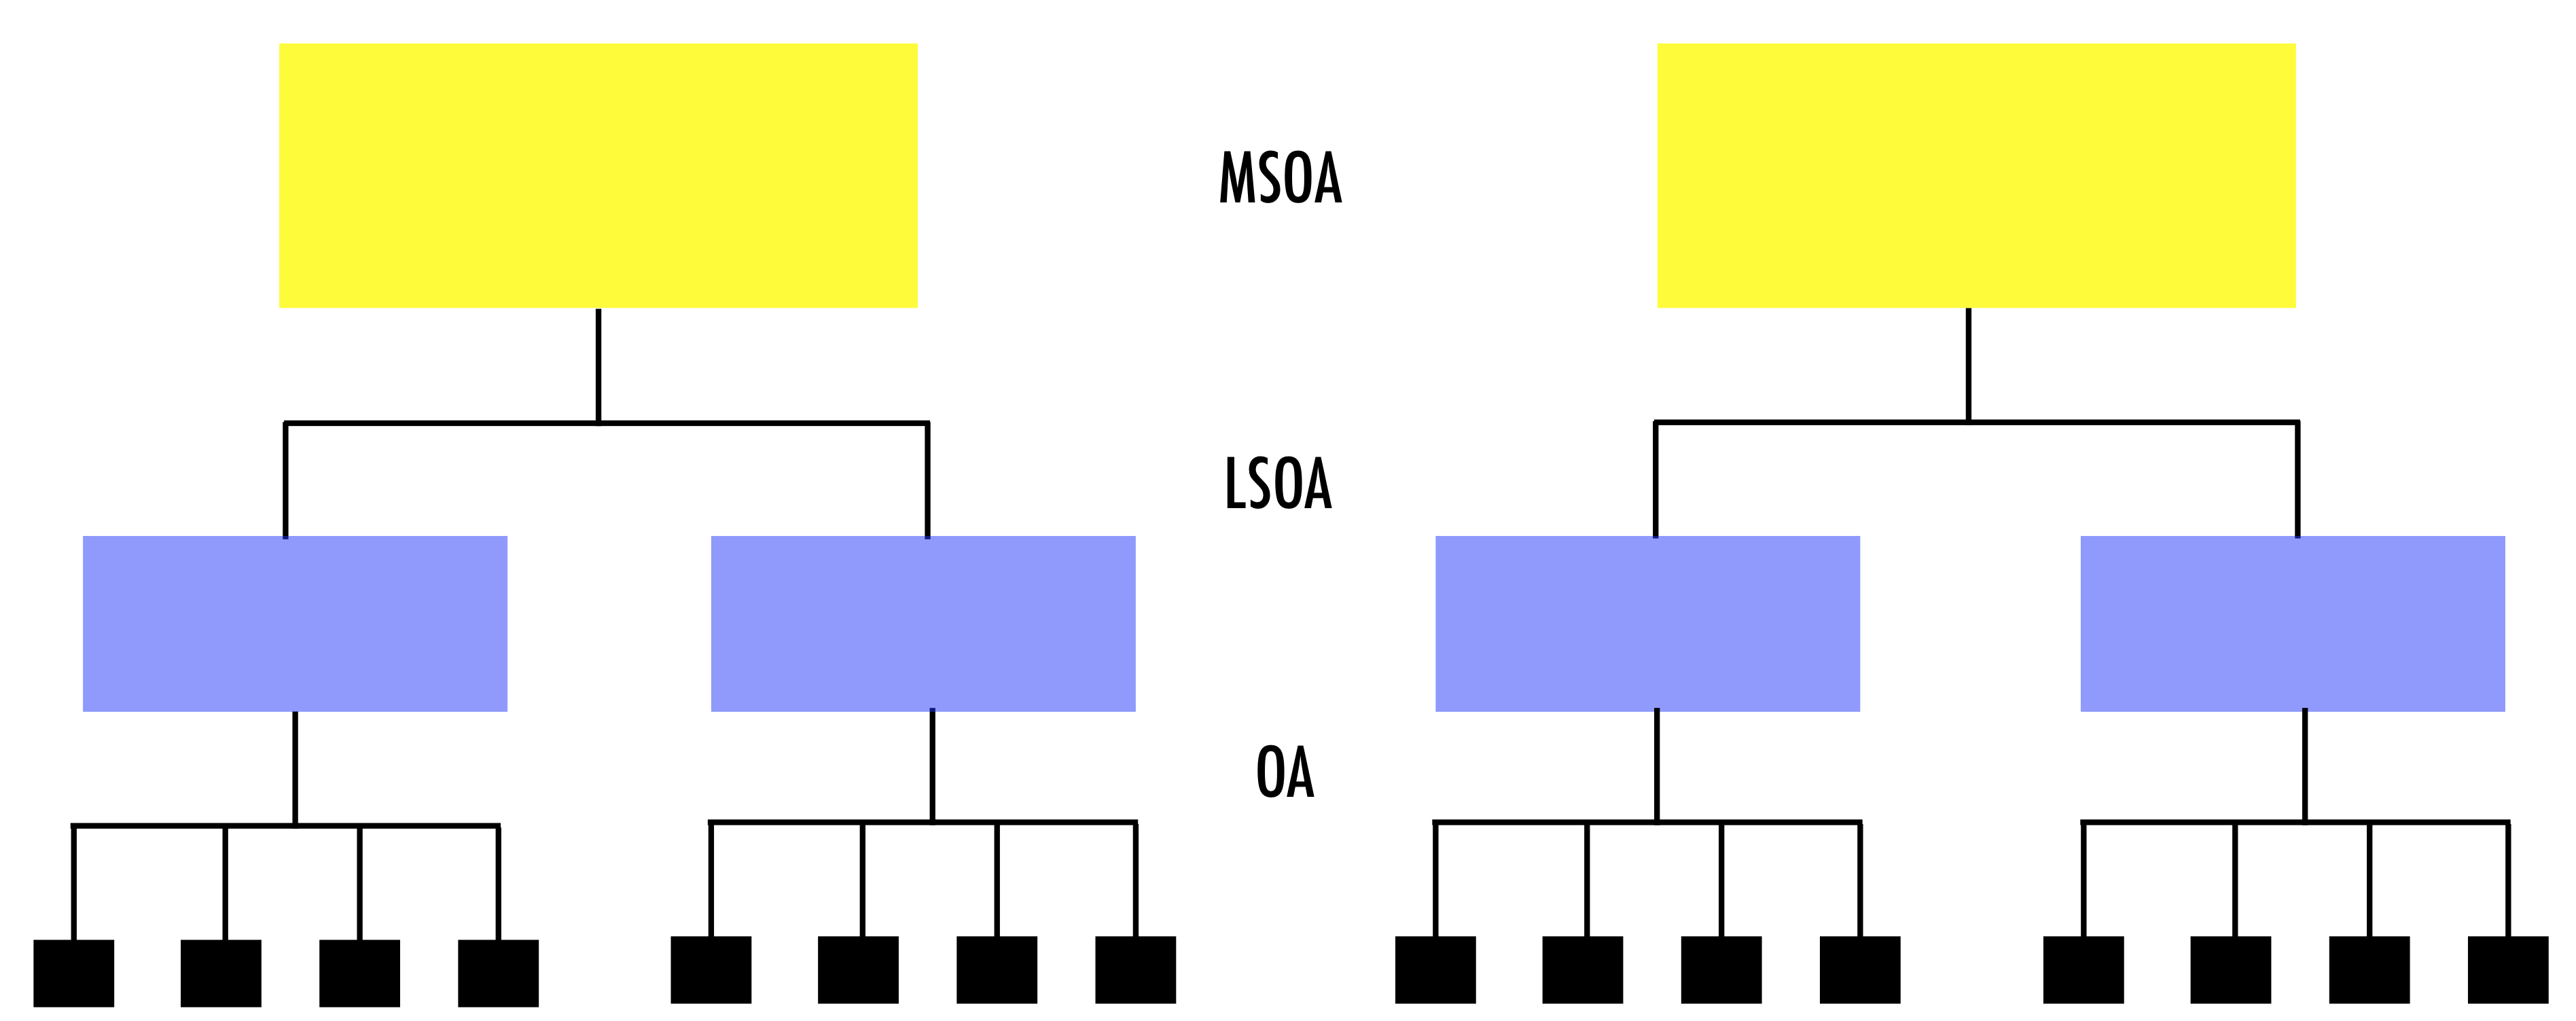
\includegraphics{figs/ch5/datastr.png}

}

\caption{Fig. 1. Data Structure.}

\end{figure}%

The data are hierarchically structured: OAs nested within LSOAs; LSOAs
nested within MSOAs; and, MSOAs nested within LADs. Observations nested
within higher geographical units may be correlated.

This is one type of hierarchical structure. There is a range of data
structures:

\begin{itemize}
\item
  Strict nested data structures eg. an individual unit is nested within
  only one higher unit
\item
  Repeated measures structures eg. various measurements for an
  individual unit
\item
  Crossed classified structures eg. individuals may work and live in
  different neighbourhoods
\item
  Multiple membership structure eg. individuals may have two different
  work places
\end{itemize}

\emph{Why should we care about the structure of the data?}

\begin{itemize}
\item
  \emph{Draw correct statistical inference}: Failing to recognise
  hierarchical structures will lead to underestimated standard errors of
  regression coefficients and an overstatement of statistical
  significance. Standard errors for the coefficients of higher-level
  predictor variables will be the most affected by ignoring grouping.
\item
  \emph{Link context to individual units}: We can link and understand
  the extent of group effects on individual outcomes eg. how belonging
  to a certain socio-economic group influences on future career
  opportunities.
\item
  \emph{Spatial dependency}: Recognising the hierarchical structure of
  data may help mitigate the effects of severe spatial autocorrelation.
\end{itemize}

Quickly, let us get a better idea about the data and look at the number
of OAs nested within LSOAs and MSOAs

\begin{Shaded}
\begin{Highlighting}[]
\CommentTok{\# mean of nested OAs within LSOAs and MSOAs}
\NormalTok{lsoa\_cd }\SpecialCharTok{\%\textgreater{}\%} \FunctionTok{table}\NormalTok{() }\SpecialCharTok{\%\textgreater{}\%}
  \FunctionTok{mean}\NormalTok{() }\SpecialCharTok{\%\textgreater{}\%}
  \FunctionTok{round}\NormalTok{(, }\DecValTok{2}\NormalTok{)}
\end{Highlighting}
\end{Shaded}

\begin{verbatim}
[1] 5
\end{verbatim}

\begin{Shaded}
\begin{Highlighting}[]
\NormalTok{msoa\_cd }\SpecialCharTok{\%\textgreater{}\%} \FunctionTok{table}\NormalTok{() }\SpecialCharTok{\%\textgreater{}\%}
  \FunctionTok{mean}\NormalTok{() }\SpecialCharTok{\%\textgreater{}\%}
  \FunctionTok{round}\NormalTok{(, }\DecValTok{2}\NormalTok{)}
\end{Highlighting}
\end{Shaded}

\begin{verbatim}
[1] 26
\end{verbatim}

\begin{Shaded}
\begin{Highlighting}[]
\CommentTok{\# number of OAs nested within LSOAs and MSOAs}
\NormalTok{lsoa\_cd }\SpecialCharTok{\%\textgreater{}\%} \FunctionTok{table}\NormalTok{() }\SpecialCharTok{\%\textgreater{}\%}
  \FunctionTok{sort}\NormalTok{() }\SpecialCharTok{\%\textgreater{}\%}
  \FunctionTok{plot}\NormalTok{()}
\end{Highlighting}
\end{Shaded}

\includegraphics{07-multilevel-01_files/figure-pdf/unnamed-chunk-5-1.pdf}

\begin{Shaded}
\begin{Highlighting}[]
\NormalTok{msoa\_cd }\SpecialCharTok{\%\textgreater{}\%} \FunctionTok{table}\NormalTok{() }\SpecialCharTok{\%\textgreater{}\%}
  \FunctionTok{sort}\NormalTok{() }\SpecialCharTok{\%\textgreater{}\%}
  \FunctionTok{plot}\NormalTok{()}
\end{Highlighting}
\end{Shaded}

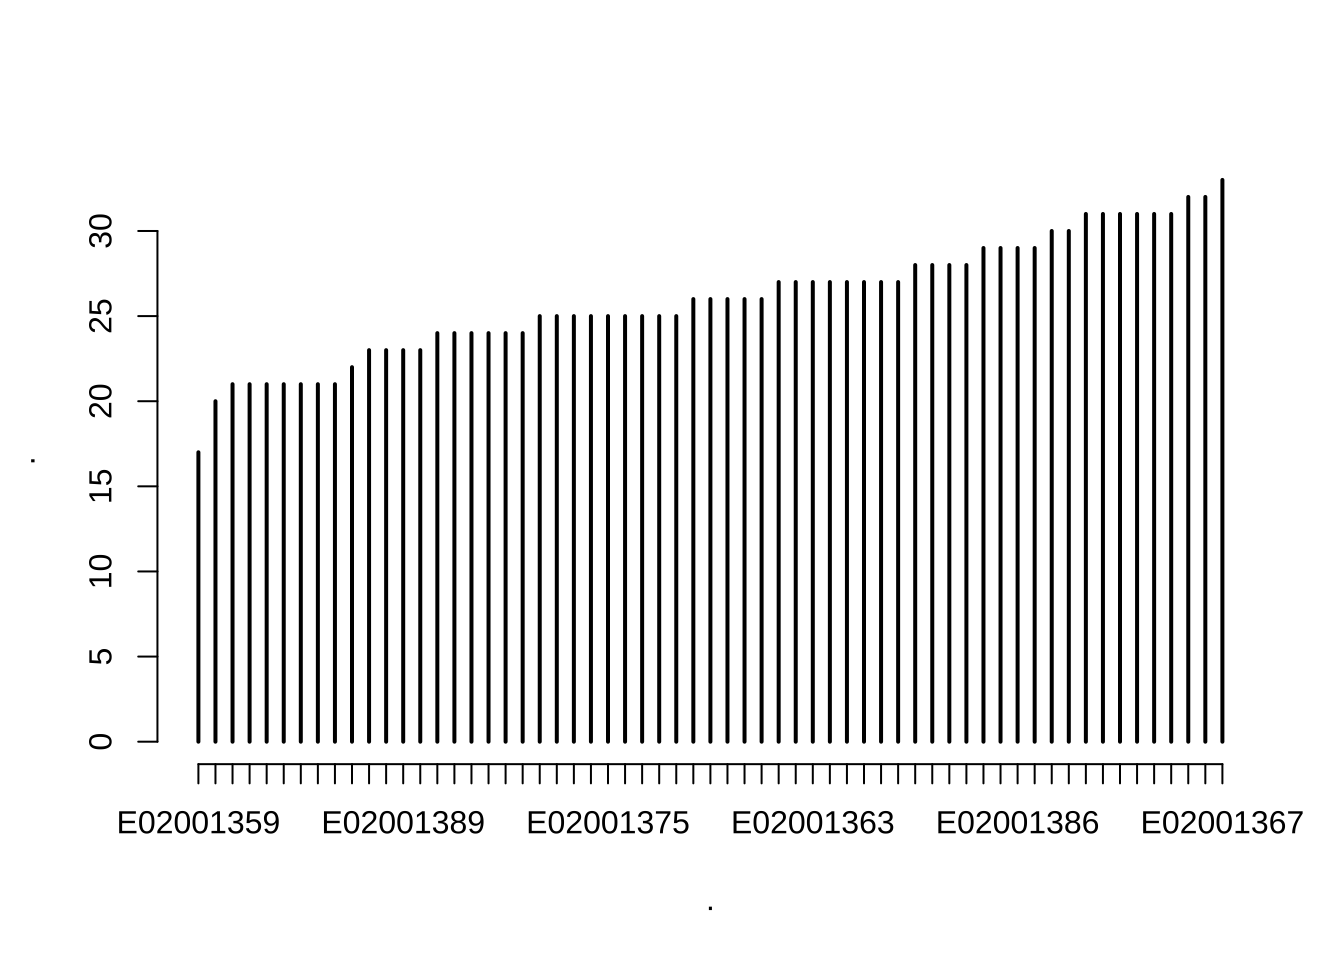
\includegraphics{07-multilevel-01_files/figure-pdf/unnamed-chunk-5-2.pdf}

\section{Modelling}\label{modelling}

We should now be persuaded that ignoring the hierarchical structure of
data may be a major issue. Let us now use a simple example to understand
the intuition of multilevel model using the census data. We will seek to
understand the spatial distribution of the proportion of population in
unemployment in Liverpool, particularly why and where concentrations in
this proportion occur. To illustrate the advantages of taking a
multilevel modelling approach, we will start by estimating a linear
regression model and progressively building complexity. We will first
estimate a model and then explain the intuition underpinning the
process. We will seek to gain a general understanding of multilevel
modelling. If you are interested in the statistical and mathemathical
formalisation of the underpinning concepts, please refer to Gelman and
Hill (2006).

We first need to want to understand our dependent variable: its density
ditribution;

\begin{Shaded}
\begin{Highlighting}[]
\FunctionTok{ggplot}\NormalTok{(}\AttributeTok{data =}\NormalTok{ oa\_shp) }\SpecialCharTok{+}
  \FunctionTok{geom\_density}\NormalTok{(}\AttributeTok{alpha=}\FloatTok{0.8}\NormalTok{, }\AttributeTok{colour=}\StringTok{"black"}\NormalTok{, }\AttributeTok{fill=}\StringTok{"lightblue"}\NormalTok{, }\FunctionTok{aes}\NormalTok{(}\AttributeTok{x =}\NormalTok{ unemp)) }\SpecialCharTok{+}
   \FunctionTok{theme\_plot\_tufte}\NormalTok{()}
\end{Highlighting}
\end{Shaded}

\includegraphics{07-multilevel-01_files/figure-pdf/unnamed-chunk-6-1.pdf}

\begin{Shaded}
\begin{Highlighting}[]
\FunctionTok{summary}\NormalTok{(unemp)}
\end{Highlighting}
\end{Shaded}

\begin{verbatim}
   Min. 1st Qu.  Median    Mean 3rd Qu.    Max. 
0.00000 0.05797 0.10256 0.11581 0.16129 0.50000 
\end{verbatim}

and, its spatial distribution:

\begin{Shaded}
\begin{Highlighting}[]
\CommentTok{\# ensure geometry is valid}
\NormalTok{oa\_shp }\OtherTok{=}\NormalTok{ sf}\SpecialCharTok{::}\FunctionTok{st\_make\_valid}\NormalTok{(oa\_shp)}

\CommentTok{\# create a map}
\NormalTok{legend\_title }\OtherTok{=} \FunctionTok{expression}\NormalTok{(}\StringTok{"\% unemployment"}\NormalTok{)}
\NormalTok{map\_oa }\OtherTok{=} \FunctionTok{tm\_shape}\NormalTok{(oa\_shp) }\SpecialCharTok{+}
  \FunctionTok{tm\_fill}\NormalTok{(}\AttributeTok{col =} \StringTok{"unemp"}\NormalTok{, }\AttributeTok{title =}\NormalTok{ legend\_title, }\AttributeTok{palette =} \FunctionTok{magma}\NormalTok{(}\DecValTok{256}\NormalTok{, }\AttributeTok{begin =} \FloatTok{0.25}\NormalTok{, }\AttributeTok{end =} \DecValTok{1}\NormalTok{), }\AttributeTok{style =} \StringTok{"cont"}\NormalTok{) }\SpecialCharTok{+} 
  \FunctionTok{tm\_borders}\NormalTok{(}\AttributeTok{col =} \StringTok{"white"}\NormalTok{, }\AttributeTok{lwd =}\NormalTok{ .}\DecValTok{01}\NormalTok{)  }\SpecialCharTok{+} 
  \FunctionTok{tm\_compass}\NormalTok{(}\AttributeTok{type =} \StringTok{"arrow"}\NormalTok{, }\AttributeTok{position =} \FunctionTok{c}\NormalTok{(}\StringTok{"right"}\NormalTok{, }\StringTok{"top"}\NormalTok{) , }\AttributeTok{size =} \DecValTok{4}\NormalTok{) }\SpecialCharTok{+} 
  \FunctionTok{tm\_scale\_bar}\NormalTok{(}\AttributeTok{breaks =} \FunctionTok{c}\NormalTok{(}\DecValTok{0}\NormalTok{,}\DecValTok{1}\NormalTok{,}\DecValTok{2}\NormalTok{), }\AttributeTok{text.size =} \FloatTok{0.5}\NormalTok{, }\AttributeTok{position =}  \FunctionTok{c}\NormalTok{(}\StringTok{"center"}\NormalTok{, }\StringTok{"bottom"}\NormalTok{)) }
\NormalTok{map\_oa}
\end{Highlighting}
\end{Shaded}

\includegraphics{07-multilevel-01_files/figure-pdf/unnamed-chunk-8-1.pdf}

Let us look at those areas:

\begin{Shaded}
\begin{Highlighting}[]
\CommentTok{\# high \%s}
\NormalTok{oa\_shp }\SpecialCharTok{\%\textgreater{}\%} \FunctionTok{filter}\NormalTok{(unemp }\SpecialCharTok{\textgreater{}} \FloatTok{0.2}\NormalTok{) }\SpecialCharTok{\%\textgreater{}\%} 
\NormalTok{  dplyr}\SpecialCharTok{::}\FunctionTok{select}\NormalTok{(oa\_cd, pop, unemp) }
\end{Highlighting}
\end{Shaded}

\begin{verbatim}
Simple feature collection with 203 features and 3 fields
Geometry type: POLYGON
Dimension:     XY
Bounding box:  xmin: 333993.8 ymin: 379748.5 xmax: 345600.2 ymax: 397681.5
Projected CRS: Transverse_Mercator
First 10 features:
       oa_cd pop     unemp                       geometry
1  E00032992 240 0.2519685 POLYGON ((335804.9 389421.6...
2  E00033008 345 0.2636364 POLYGON ((335080 388528, 33...
3  E00033074 299 0.2075472 POLYGON ((336947.3 387766.7...
4  E00033075 254 0.2288136 POLYGON ((336753.6 387465.2...
5  E00033080 197 0.2647059 POLYGON ((338196 387079, 33...
6  E00033103 298 0.2148148 POLYGON ((340484 385429.6, ...
7  E00033116 190 0.2156863 POLYGON ((341960.7 386422.1...
8  E00033134 190 0.2674419 POLYGON ((337137 393089.6, ...
9  E00033137 289 0.2661290 POLYGON ((337363.8 392122.4...
10 E00033138 171 0.3561644 POLYGON ((337481.5 392166.2...
\end{verbatim}

\subsection{Baseline Linear Regression
Model}\label{baseline-linear-regression-model}

Now let us estimate a simple linear regression model with the intercept
only:

\begin{Shaded}
\begin{Highlighting}[]
\CommentTok{\# specify a model equation}
\NormalTok{eq1 }\OtherTok{\textless{}{-}}\NormalTok{ unemp }\SpecialCharTok{\textasciitilde{}} \DecValTok{1}
\NormalTok{model1 }\OtherTok{\textless{}{-}} \FunctionTok{lm}\NormalTok{(}\AttributeTok{formula =}\NormalTok{ eq1, }\AttributeTok{data =}\NormalTok{ oa\_shp)}

\CommentTok{\# estimates}
\FunctionTok{summary}\NormalTok{(model1)}
\end{Highlighting}
\end{Shaded}

\begin{verbatim}

Call:
lm(formula = eq1, data = oa_shp)

Residuals:
     Min       1Q   Median       3Q      Max 
-0.11581 -0.05784 -0.01325  0.04548  0.38419 

Coefficients:
            Estimate Std. Error t value Pr(>|t|)    
(Intercept) 0.115812   0.001836   63.09   <2e-16 ***
---
Signif. codes:  0 '***' 0.001 '**' 0.01 '*' 0.05 '.' 0.1 ' ' 1

Residual standard error: 0.07306 on 1583 degrees of freedom
\end{verbatim}

To understand the differences between the linear regression model and
multilevel models, let us consider the model we have estimated:

\[y_{i} = \beta_{0} + e_{i}\] where \(y_{i}\) represents the proportion
of the unemployed resident population in the OA \(i\); \(\beta_{0}\) is
the regression intercept and measures the average proportion of the
unemployed resident population across OAs; and, \(e_{i}\) is the error
term. But how do we deal with the hierarchical structure of the data?

\subsubsection{Limitations}\label{limitations}

Before looking at the answer, let's first understand some of the key
limitations of the linear regression model to handle the hierarchical
structure of data. A key limitation of the linear regression model is
that it only captures average relationships in the data. It does not
capture variations in the relationship between variables across areas or
groups. Another key limitation is that the linear regression model can
capture associations at either macro or micro levels, but it does not
simultaneously measure their interdependencies.

To illustrate this, let us consider the regression intercept. It
indicates that the average percentage of unemployed population at the OA
level is 0.12 but this model ignores any spatial clustering ie. the
percentage of unemployed population tends to be similar across OAs
nested within a same LSOA or MSOA. A side effect of ignoring this is
that our standard errors are biased, and thus claims about statistical
significance based on them would be misleading. Additionally, this
situation also means we cannot explore variations in the percentage of
unemployed population across LSOAs or MSOAs ie. how the percentage of
unemployed population may be dependent on various contextual factors at
these geographical scales.

\subsubsection{Fixed Effect Approach}\label{fixed-effect-approach}

An alternative approach is to adopt a fixed effects approach, or
no-pooling model; that is, adding dummy variables indicating the group
classification into the regression model eg. the way OAs is nested
within LSOAs (or MSOAs). This approach has limitations. First, there is
high risk of overfitting. The number of groups may be too large,
relative to the number of observations. Second, the estimation of
multiple parameters may be required so that measuring differences
between groups may be challenging. Third, a fixed effects approach does
not allow including group-level explanatory variables. You can try
fitting a linear regression model extending our estimated model to
include dummy variables for individual LSOAs (and/or MSOAs) so you can
compare this to the multilevel model below.

An alternative is fitting separate linear regression models for each
group. This approach is not always possible if there are groups with
small sizes.

\section{Multilevel Modelling: Random Intercept
Model}\label{multilevel-modelling-random-intercept-model}

We use multilevel modelling to account for the hierarchical nature of
the data by explicitly recognising that OAs are nested within LSOAs and
MSOAs. Multilevel models can easily be estimated using in R using the
package \texttt{lme4}. We implement an two-level model to allow for
variation across LSOAs. We estimate an only intercept model allowing for
variation across LSOAs. In essence, we are estimating a model with
varying intercept coefficient by LSOA. As you can see in the code chunk
below, the equation has an additional component. This is the group
component or LSOA effect. The \texttt{(1\ \textbar{}\ lsoa\_cd)} means
that we are allowing the intercept, represented by 1, to vary by LSOA.

\begin{Shaded}
\begin{Highlighting}[]
\CommentTok{\# specify a model equation}
\NormalTok{eq2 }\OtherTok{\textless{}{-}}\NormalTok{ unemp }\SpecialCharTok{\textasciitilde{}} \DecValTok{1} \SpecialCharTok{+}\NormalTok{ (}\DecValTok{1} \SpecialCharTok{|}\NormalTok{ lsoa\_cd)}
\NormalTok{model2 }\OtherTok{\textless{}{-}} \FunctionTok{lmer}\NormalTok{(eq2, }\AttributeTok{data =}\NormalTok{ oa\_shp)}

\CommentTok{\# estimates}
\FunctionTok{summary}\NormalTok{(model2)}
\end{Highlighting}
\end{Shaded}

\begin{verbatim}
Linear mixed model fit by REML ['lmerMod']
Formula: unemp ~ 1 + (1 | lsoa_cd)
   Data: oa_shp

REML criterion at convergence: -4382.6

Scaled residuals: 
    Min      1Q  Median      3Q     Max 
-2.8741 -0.5531 -0.1215  0.4055  5.8207 

Random effects:
 Groups   Name        Variance Std.Dev.
 lsoa_cd  (Intercept) 0.002701 0.05197 
 Residual             0.002575 0.05074 
Number of obs: 1584, groups:  lsoa_cd, 298

Fixed effects:
            Estimate Std. Error t value
(Intercept) 0.114316   0.003277   34.89
\end{verbatim}

We can estimate a three-level model by replacing
\texttt{(1\ \textbar{}\ lsoa\_cd)} for
\texttt{(1\ \textbar{}\ msoa\_cd/lsoa\_cd)} to allow the intercept to
also vary by MSOAs and account for the nesting structure of LSOAs within
MSOAs. In multilevel modelling, these types of models are formally known
as \emph{nested random effects} and they differ from a different set of
models known as \emph{crossed random effects}.

::: column-margin ::: callout-note A crossed random effect model in our
example would be expressed as follows:

\texttt{unemp\ \textasciitilde{}\ 1\ +\ (1\ \textbar{}\ lsoa\_cd)\ +\ (1\ \textbar{}\ msoa\_cd)}

::: ::: column-margin

\begin{Shaded}
\begin{Highlighting}[]
\CommentTok{\# specify a model equation}
\NormalTok{eq3 }\OtherTok{\textless{}{-}}\NormalTok{ unemp }\SpecialCharTok{\textasciitilde{}} \DecValTok{1} \SpecialCharTok{+}\NormalTok{ (}\DecValTok{1} \SpecialCharTok{|}\NormalTok{ msoa\_cd}\SpecialCharTok{/}\NormalTok{lsoa\_cd)}
\NormalTok{model3 }\OtherTok{\textless{}{-}} \FunctionTok{lmer}\NormalTok{(eq3, }\AttributeTok{data =}\NormalTok{ oa\_shp)}

\CommentTok{\# estimates}
\FunctionTok{summary}\NormalTok{(model3)}
\end{Highlighting}
\end{Shaded}

\begin{verbatim}
Linear mixed model fit by REML ['lmerMod']
Formula: unemp ~ 1 + (1 | msoa_cd/lsoa_cd)
   Data: oa_shp

REML criterion at convergence: -4529.3

Scaled residuals: 
    Min      1Q  Median      3Q     Max 
-2.5624 -0.5728 -0.1029  0.4228  6.1363 

Random effects:
 Groups          Name        Variance  Std.Dev.
 lsoa_cd:msoa_cd (Intercept) 0.0007603 0.02757 
 msoa_cd         (Intercept) 0.0020735 0.04554 
 Residual                    0.0025723 0.05072 
Number of obs: 1584, groups:  lsoa_cd:msoa_cd, 298; msoa_cd, 61

Fixed effects:
            Estimate Std. Error t value
(Intercept) 0.115288   0.006187   18.64
\end{verbatim}

We see two sets of coefficients: \emph{fixed effects} and \emph{random
effects}. \emph{Fixed effects} correspond to the standard linear
regression coefficients. Their interpretation is as usual. \emph{Random
effects} are the novelty. It is a term in multilevel modelling and
refers to varying coefficients i.e.~the randomness in the probability of
the model for the group-level coefficients. Specifically they relate to
estimates of the average variance and standard deviation within groups
(i.e.~LSOAs or MSOAs). Intiutively, variance and standard deviation
indicate the extent to which the intercept, on average, varies by LSOAs
and MSOAs.

\begin{figure}[H]

{\centering 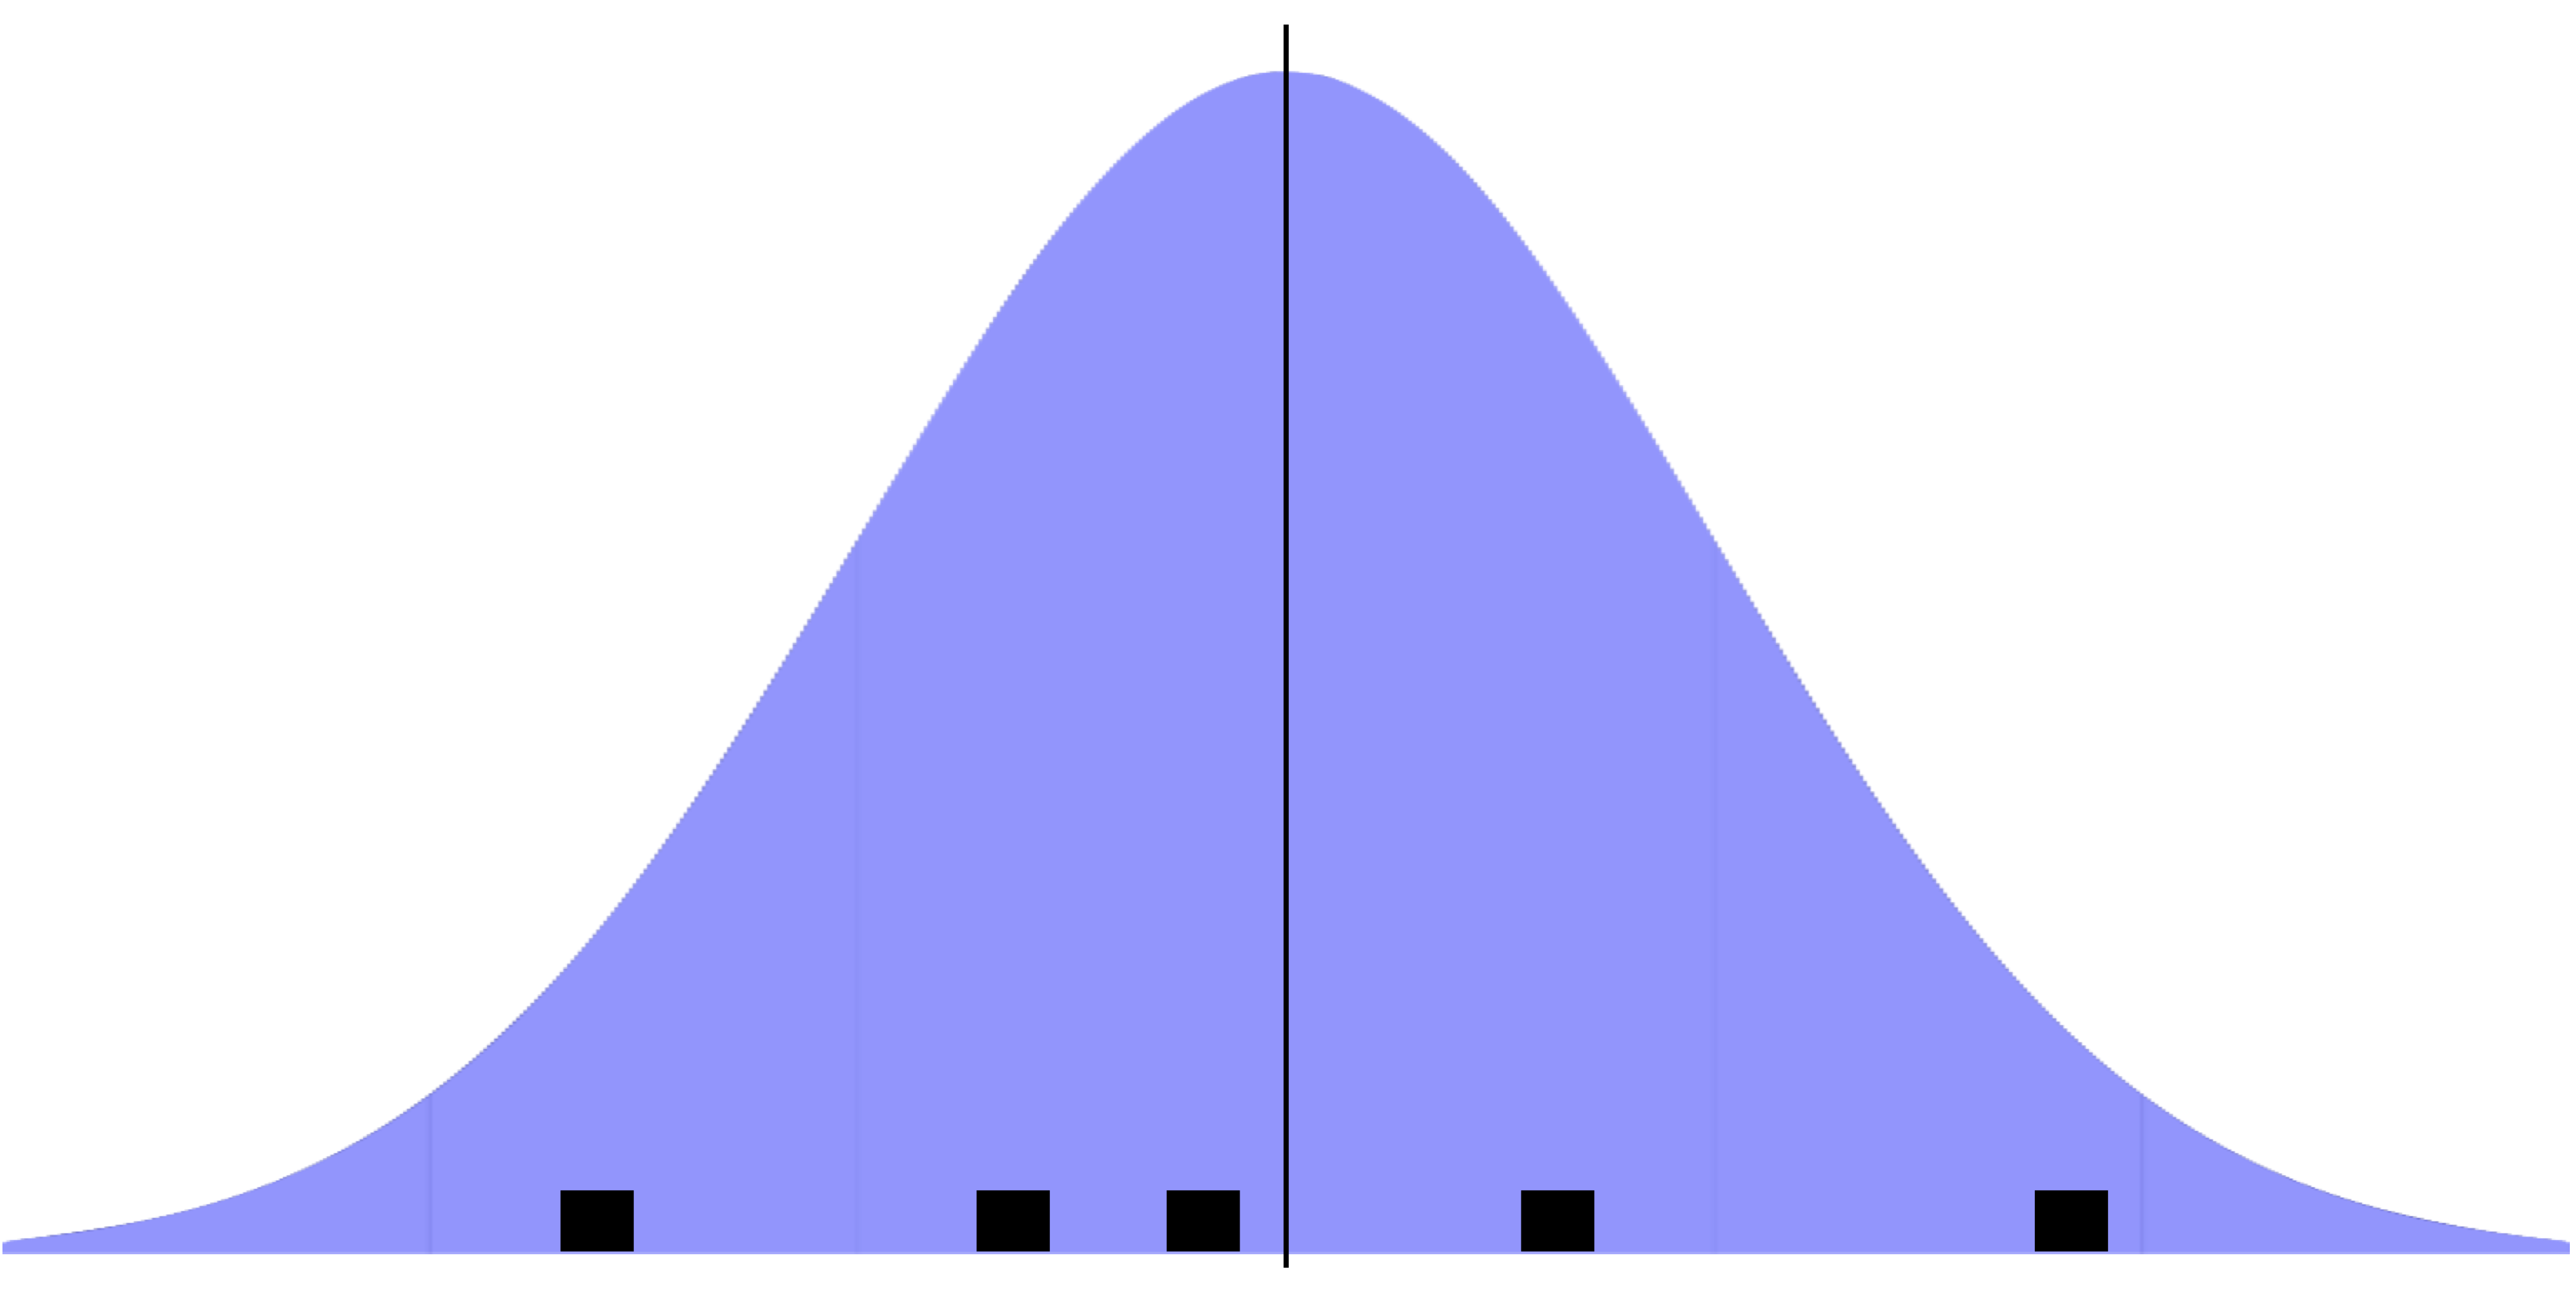
\includegraphics{figs/ch5/nm_dist_obs.png}

}

\caption{Fig. 2. Variation of observations around their level 1 group
mean.}

\end{figure}%%
\begin{figure}[H]

{\centering 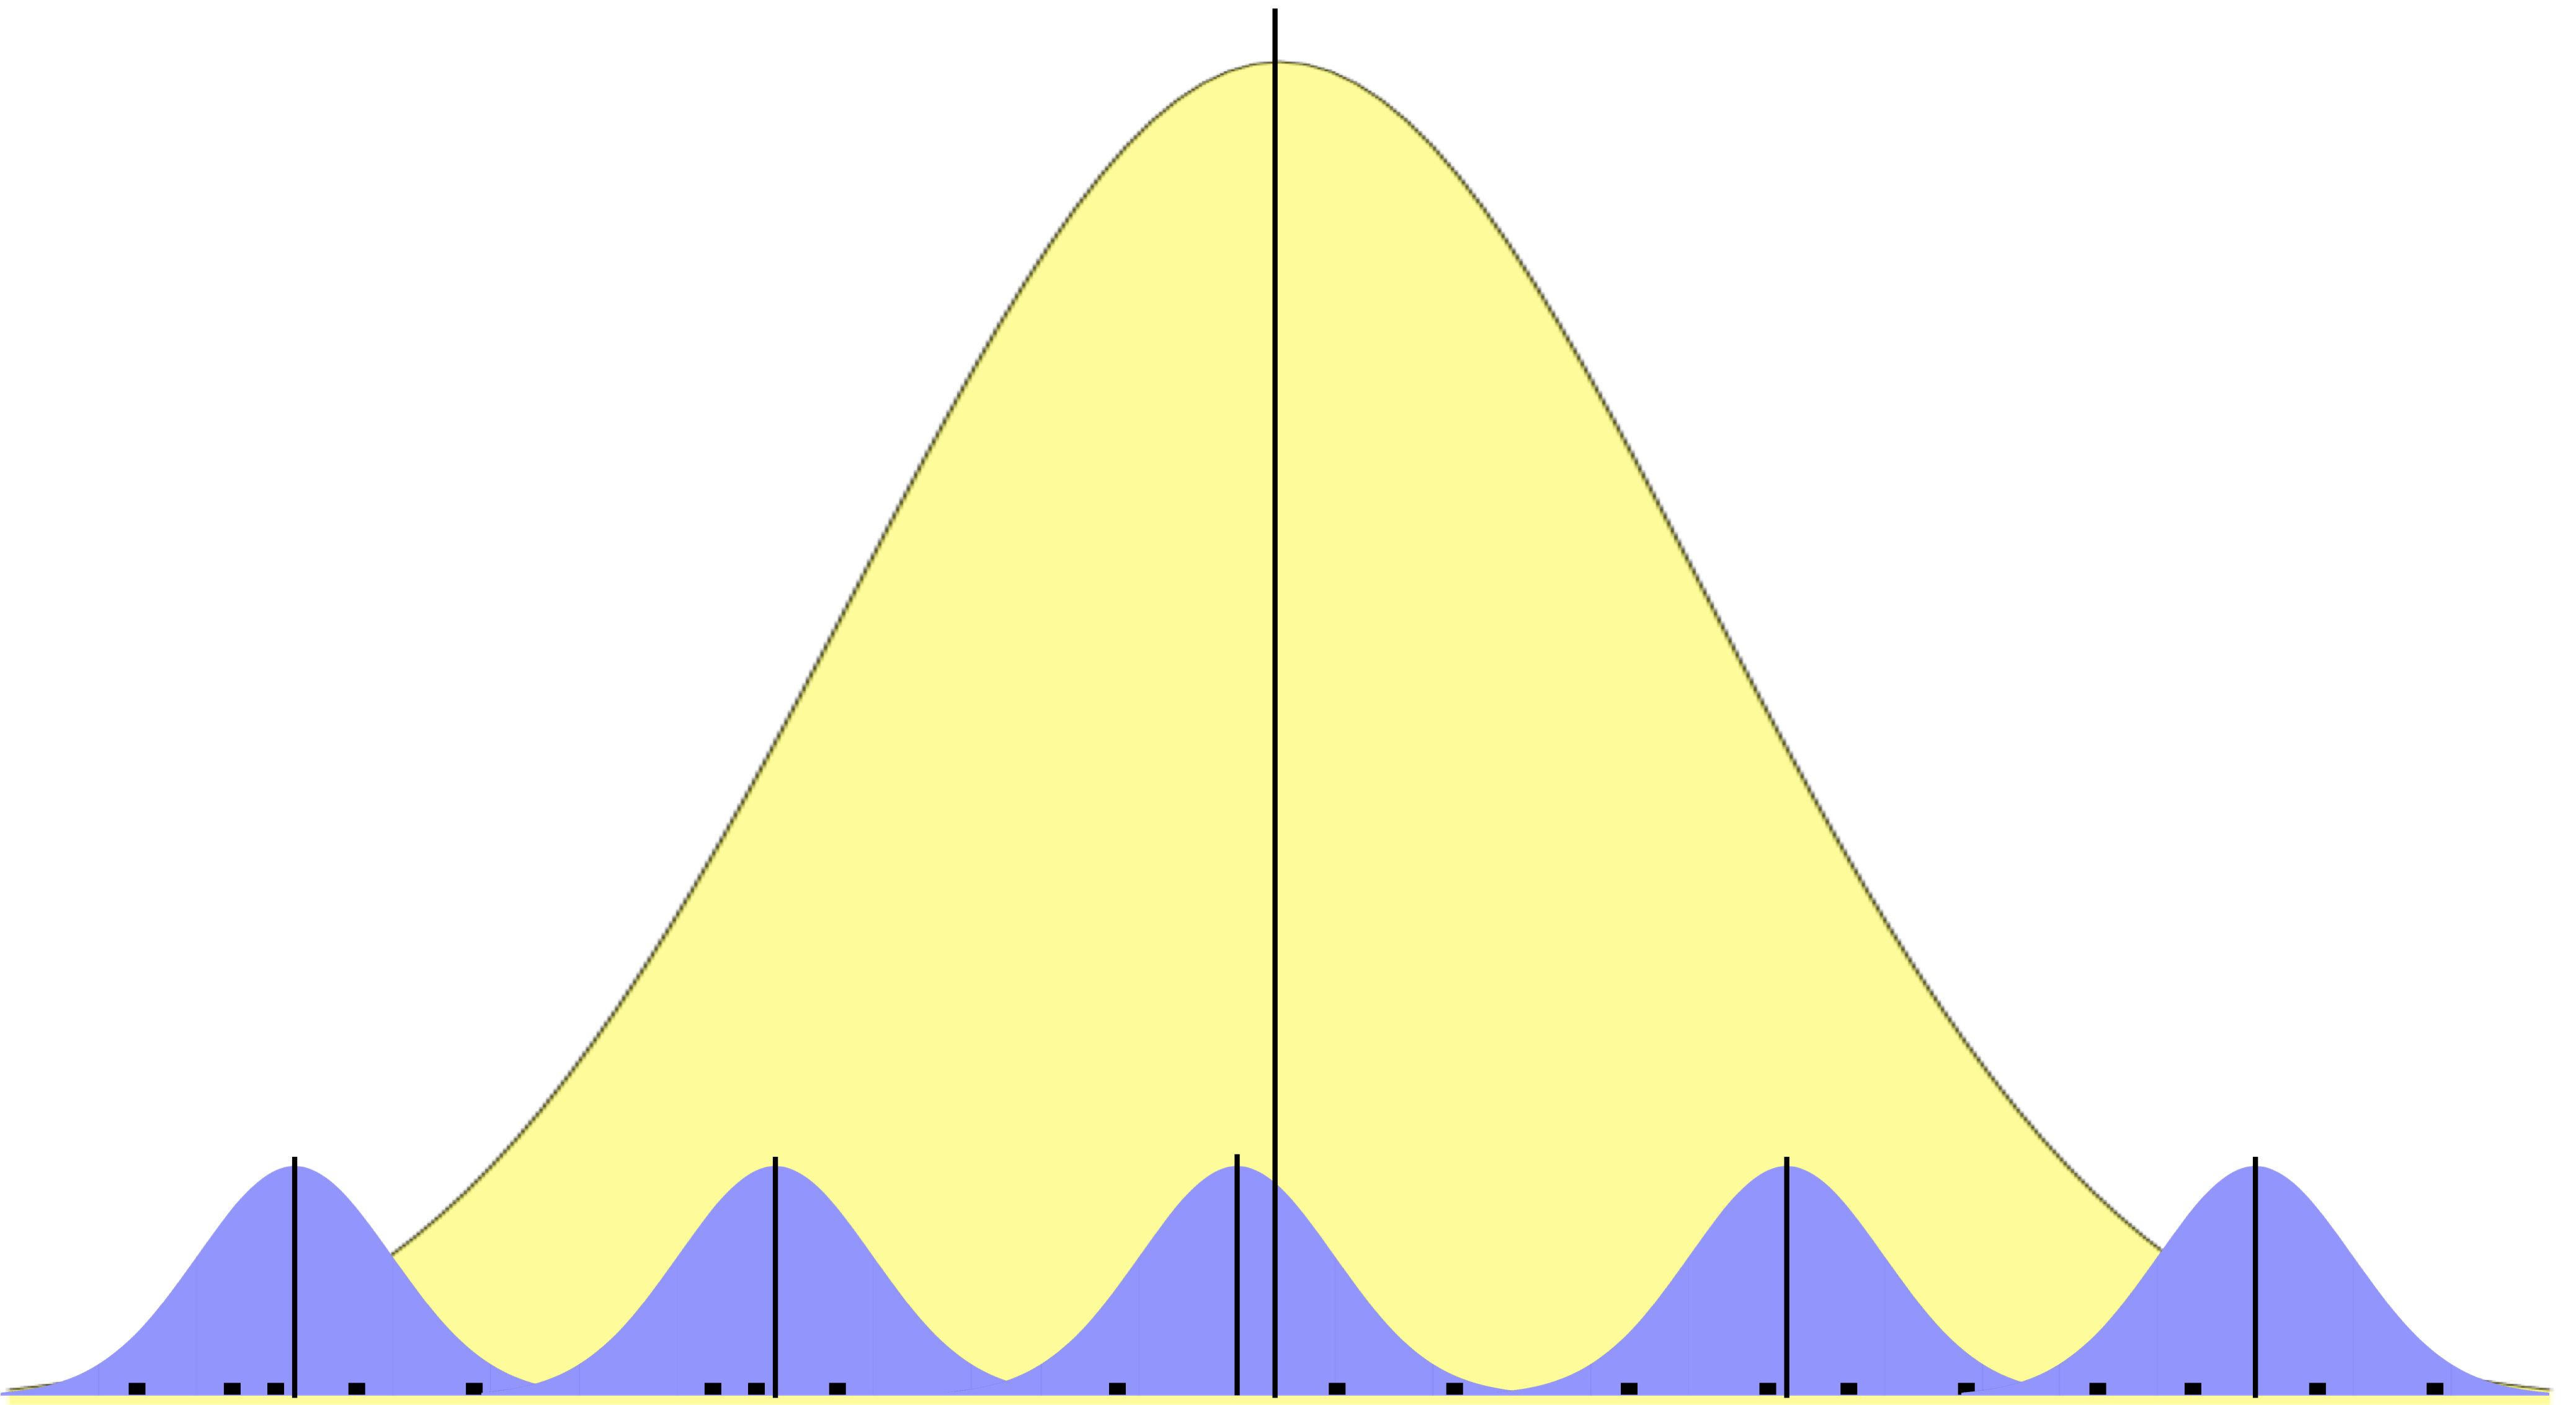
\includegraphics{figs/ch5/nm_dist_msoa.png}

}

\caption{Fig. 3. Variation of level 1 group mean around their level 2
group mean.}

\end{figure}%%
\begin{figure}[H]

{\centering 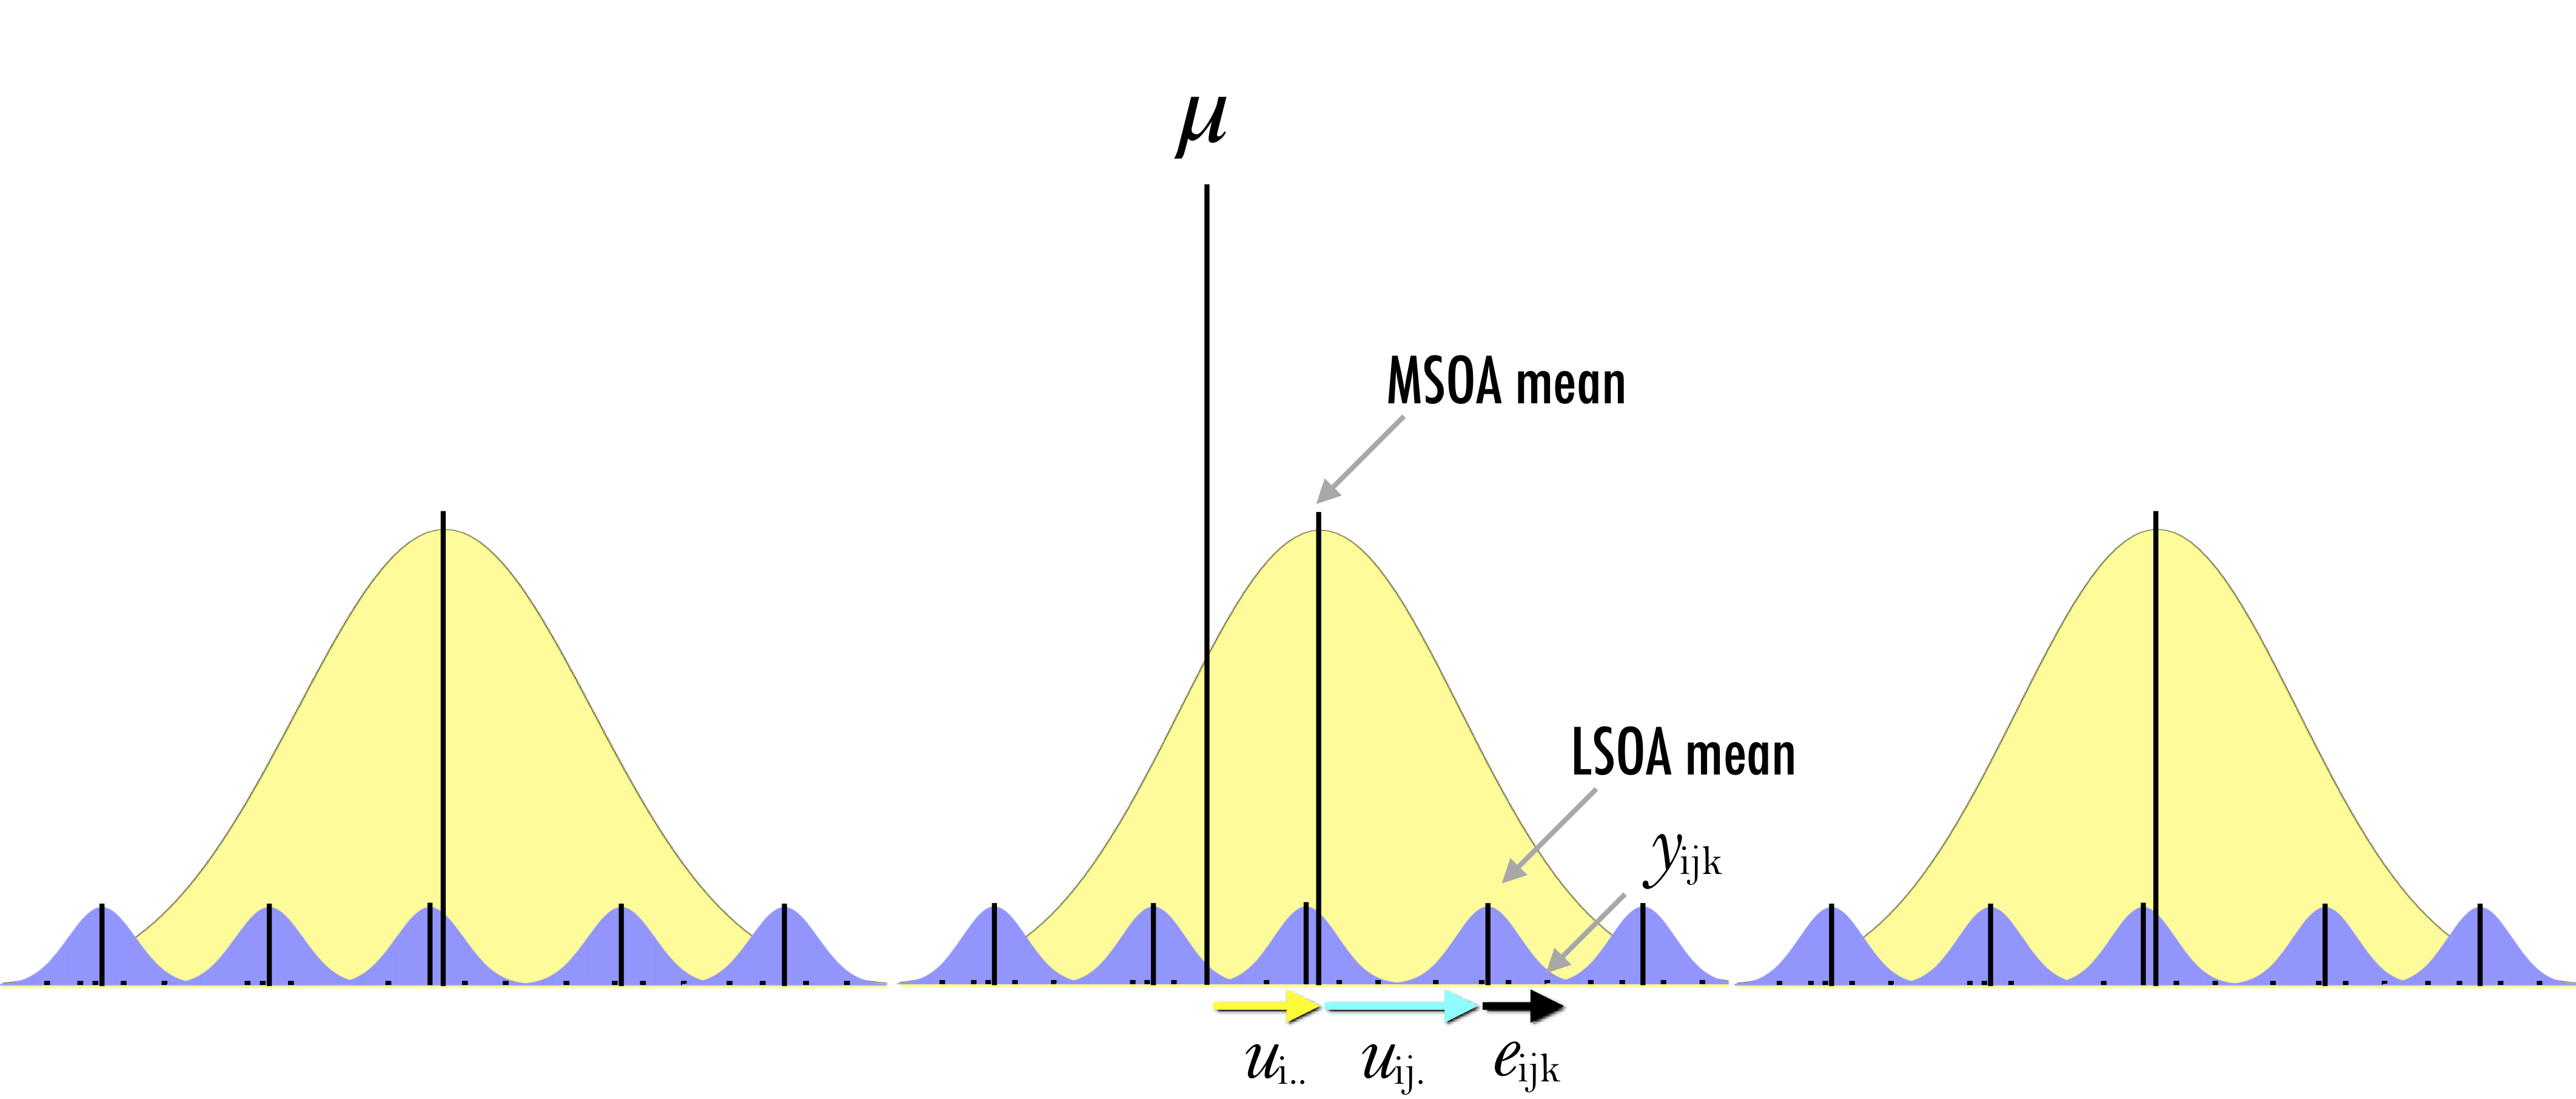
\includegraphics{figs/ch5/nm_dist_grand.png}

}

\caption{Fig. 4. Grand mean.}

\end{figure}%

More formally, we first estimated the simplest regression model which is
an intercept-only model and equivalent to the sample mean (i.e.~the
\emph{fixed} part of the model):

\[y_{ijk} = \mu + e_{ijk}\] and then we made the \emph{random} part of
the model (\(e_{ijk}\)) more complex to account for the hierarchical
structure of the data by estimating the following three-level regression
model:

\[y_{ijk} = \mu + u_{i..} + u_{ij.} + e_{ijk}\]

where \(y_{ijk}\) represents the proportion of unemployed population in
OA \(i\) nested within LSOA \(j\) and MSOA \(k\); \(\mu\) represents the
sample mean and the \emph{fixed} part of the model; \(e_{ijk}\) is the
deviation of an observation from its LSOA mean; \(u_{ij.}\) is the
deviation of the LSOA mean from its MSOA mean; \(u_{i..}\) is the
deviation of the MSOA mean from the fixed part of the model \(\mu\).
Conceptually, this model is decomposing the variance of the model in
terms of the hierarchical structure of the data. It is partitioning the
observation's residual into three parts or \emph{variance components}.
These components measure the relative extent of variation of each
hierarchical level ie. LSOA, MSOA and grand means. To estimate the set
of residuals, they are assumed to follow a normal distribution and are
obtained after fitting the model and are based on the estimates of the
model parameters (i.e.~intercept and variances of the random
parameters).

Let's now return to our three-level model (reported again below), we see
that the intercept or fixed part of the model is the same as for the
linear regression. The multilevel model reports greater standard errors.
Multilevel models capture the hierarchical structure of the data and
thus more precisely estimate the standard errors for our parameters.

\begin{Shaded}
\begin{Highlighting}[]
\CommentTok{\# report model 3}
\FunctionTok{summary}\NormalTok{(model3)}
\end{Highlighting}
\end{Shaded}

\begin{verbatim}
Linear mixed model fit by REML ['lmerMod']
Formula: unemp ~ 1 + (1 | msoa_cd/lsoa_cd)
   Data: oa_shp

REML criterion at convergence: -4529.3

Scaled residuals: 
    Min      1Q  Median      3Q     Max 
-2.5624 -0.5728 -0.1029  0.4228  6.1363 

Random effects:
 Groups          Name        Variance  Std.Dev.
 lsoa_cd:msoa_cd (Intercept) 0.0007603 0.02757 
 msoa_cd         (Intercept) 0.0020735 0.04554 
 Residual                    0.0025723 0.05072 
Number of obs: 1584, groups:  lsoa_cd:msoa_cd, 298; msoa_cd, 61

Fixed effects:
            Estimate Std. Error t value
(Intercept) 0.115288   0.006187   18.64
\end{verbatim}

\subsection{Interpretation}\label{interpretation}

\begin{quote}
Fixed effects
\end{quote}

We start by examining the fixed effects or estimated model averaging
over LSOAs and MSOAs, \(y_{ijk} = 0.115288\) which can also be called by
executing:

\begin{Shaded}
\begin{Highlighting}[]
\FunctionTok{fixef}\NormalTok{(model3)}
\end{Highlighting}
\end{Shaded}

\begin{verbatim}
(Intercept) 
  0.1152881 
\end{verbatim}

Th estimated intercept indicates that the overall mean taken across
LSOAs and MSOAs is estimated as \texttt{0.1152881}.

\begin{quote}
Random effects
\end{quote}

The set of random effects contains three estimates of variance and
standard deviation and refer to the variance components discussed above.
The \texttt{lsoa\_cd:msoa\_cd}, \texttt{msoa\_cd} and \texttt{Residual}
estimates indicate that the extent of estimated LSOA-, MSOA- and
individual-level variance is \texttt{0.0007603}, \texttt{0.0020735} and
\texttt{0.0025723}, respectively.

\subsection{Variance Partition Coefficient
(VPC)}\label{variance-partition-coefficient-vpc}

The purpose of multilevel models is to partition variance in the outcome
between the different groupings in the data. We thus often want to know
the percentage of variation in the dependent variable accounted by
differences across groups i.e.~what proportion of the total variance is
attributable to variation within-groups, or how much is found
between-groups. The statistic to obtain this is termed the variance
partition coefficient (VPC), or intraclass correlation.\footnote{The VPC
  is equal to the intra-class correlation coefficient which is the
  correlation between the observations of the dependent variable
  selected randomly from the same group. For instance, if the VPC is
  0.1, we would say that 10\% of the variation is between groups and
  90\% within. The correlation between randomly chosen pairs of
  observations belonging to the same group is 0.1.} For our case, the
VPC at the MSOA level indicates that 38\% of the variation in percentage
of unemployed resident population across OAs can be explained by
differences across MSOAs.

\marginnote{\begin{footnotesize}

\begin{tcolorbox}[enhanced jigsaw, colframe=quarto-callout-tip-color-frame, leftrule=.75mm, arc=.35mm, breakable, opacityback=0, bottomrule=.15mm, colback=white, rightrule=.15mm, toprule=.15mm, left=2mm]

\textbf{Task} What is the VPC at the LSOA level?

\end{tcolorbox}

\end{footnotesize}}

\begin{Shaded}
\begin{Highlighting}[]
\NormalTok{vpc\_msoa }\OtherTok{\textless{}{-}} \FloatTok{0.0020735} \SpecialCharTok{/}\NormalTok{ (}\FloatTok{0.0007603} \SpecialCharTok{+} \FloatTok{0.0020735} \SpecialCharTok{+} \FloatTok{0.0025723}\NormalTok{)}
\NormalTok{vpc\_msoa }\SpecialCharTok{*} \DecValTok{100}
\end{Highlighting}
\end{Shaded}

\begin{verbatim}
[1] 38.35482
\end{verbatim}

You can also obtain the VPC by executing:

\begin{Shaded}
\begin{Highlighting}[]
\FunctionTok{summ}\NormalTok{(model3)}
\end{Highlighting}
\end{Shaded}

\begin{table}[!h]
\centering
\begin{tabular}{lr}
\toprule
\cellcolor{gray!10}{Observations} & \cellcolor{gray!10}{1584}\\
Dependent variable & unemp\\
\cellcolor{gray!10}{Type} & \cellcolor{gray!10}{Mixed effects linear regression}\\
\bottomrule
\end{tabular}
\end{table} \begin{table}[!h]
\centering
\begin{tabular}{lr}
\toprule
\cellcolor{gray!10}{AIC} & \cellcolor{gray!10}{-4521.26}\\
BIC & -4499.79\\
\cellcolor{gray!10}{Pseudo-R² (fixed effects)} & \cellcolor{gray!10}{0.00}\\
Pseudo-R² (total) & 0.52\\
\bottomrule
\end{tabular}
\end{table} \begin{table}[!h]
\centering
\begin{threeparttable}
\begin{tabular}{lrrrrr}
\toprule
\multicolumn{6}{c}{Fixed Effects} \\
\cmidrule(l{3pt}r{3pt}){1-6}
  & Est. & S.E. & t val. & d.f. & p\\
\midrule
\cellcolor{gray!10}{(Intercept)} & \cellcolor{gray!10}{0.12} & \cellcolor{gray!10}{0.01} & \cellcolor{gray!10}{18.63} & \cellcolor{gray!10}{59.98} & \cellcolor{gray!10}{0.00}\\
\bottomrule
\end{tabular}
\begin{tablenotes}
\item  p values calculated using Kenward-Roger standard errors and d.f. 
\end{tablenotes}
\end{threeparttable}
\end{table} \begin{table}[!h]
\centering
\begin{tabular}{lll}
\toprule
\multicolumn{3}{c}{Random Effects} \\
\cmidrule(l{3pt}r{3pt}){1-3}
Group & Parameter & Std. Dev.\\
\midrule
\cellcolor{gray!10}{lsoa\_cd:msoa\_cd} & \cellcolor{gray!10}{(Intercept)} & \cellcolor{gray!10}{0.03}\\
msoa\_cd & (Intercept) & 0.05\\
\cellcolor{gray!10}{Residual} & \cellcolor{gray!10}{} & \cellcolor{gray!10}{0.05}\\
\bottomrule
\end{tabular}
\end{table} \begin{table}[!h]
\centering
\begin{tabular}{lrl}
\toprule
\multicolumn{3}{c}{Grouping Variables} \\
\cmidrule(l{3pt}r{3pt}){1-3}
Group & \# groups & ICC\\
\midrule
\cellcolor{gray!10}{lsoa\_cd:msoa\_cd} & \cellcolor{gray!10}{298} & \cellcolor{gray!10}{0.14}\\
msoa\_cd & 61 & 0.38\\
\bottomrule
\end{tabular}
\end{table}

\subsection{Uncertainty of Estimates}\label{uncertainty-of-estimates}

You may have noticed that \texttt{lme4} does not provide p-values,
because of
\href{https://stat.ethz.ch/pipermail/r-help/2006-May/094765.html}{various
reasons} as explained by Doug Bates, one of the author of \texttt{lme4}.
These explanations mainly refer to the complexity of dealing with
varying sample sizes at a given hierarchical level. The number of
observations at each hierarchical level varies across individual
groupings (i.e.~LSOA or MSOA). It may even be one single observation.
This has implications for the distributional assumptions, denominator
degrees of freedom and how to approximate a ``best'' solution. Various
approaches exist to compute the statistical significance of estimates.
We use the \texttt{confint} function available within \texttt{lme4} to
obtain confidence intervals.

\begin{Shaded}
\begin{Highlighting}[]
\FunctionTok{confint}\NormalTok{(model3, }\AttributeTok{level =} \FloatTok{0.95}\NormalTok{)}
\end{Highlighting}
\end{Shaded}

\begin{verbatim}
Computing profile confidence intervals ...
\end{verbatim}

\begin{verbatim}
                 2.5 %     97.5 %
.sig01      0.02360251 0.03189046
.sig02      0.03707707 0.05562307
.sigma      0.04882281 0.05273830
(Intercept) 0.10307341 0.12751103
\end{verbatim}

\texttt{.sig01} refers to the LSOA level; \texttt{.sig02} refers to the
MSOA level; and, \texttt{.sigma} refers to the OA level.

\subsection{Assessing Group-level
Variation}\label{assessing-group-level-variation}

\emph{Estimated regression coefficients}

In multilevel modelling, our primary interest is in knowing differences
across groups. To visualise the estimated model within each group (ie.
LSOA and MSOA), we type:

\begin{Shaded}
\begin{Highlighting}[]
\NormalTok{coef\_m3 }\OtherTok{\textless{}{-}} \FunctionTok{coef}\NormalTok{(model3)}
\FunctionTok{head}\NormalTok{(coef\_m3}\SpecialCharTok{$}\NormalTok{lsoa\_cd,}\DecValTok{5}\NormalTok{)}
\end{Highlighting}
\end{Shaded}

\begin{verbatim}
                    (Intercept)
E01006512:E02001377  0.09915456
E01006513:E02006932  0.09889615
E01006514:E02001383  0.09297051
E01006515:E02001383  0.09803754
E01006518:E02001390  0.09642939
\end{verbatim}

The results indicate that the estimated regression line is
\(y = 0.09915456\) for LSOA \texttt{E01006512} within MSOA
\texttt{E02001377}; \(y = 0.09889615\) for LSOA \texttt{E01006513}
within MSOA \texttt{E02006932} and so forth.

\marginnote{\begin{footnotesize}

\begin{tcolorbox}[enhanced jigsaw, colframe=quarto-callout-tip-color-frame, leftrule=.75mm, arc=.35mm, breakable, opacityback=0, bottomrule=.15mm, colback=white, rightrule=.15mm, toprule=.15mm, left=2mm]

\textbf{Task} Try getting the estimated model within each MSOA.

\end{tcolorbox}

\end{footnotesize}}

\emph{Random effects}

We can look at the estimated group-level (or LSOA-level and MSOA-level)
errors; that is, \emph{random effects}:

\begin{Shaded}
\begin{Highlighting}[]
\NormalTok{ranef\_m3 }\OtherTok{\textless{}{-}} \FunctionTok{ranef}\NormalTok{(model3)}
\FunctionTok{head}\NormalTok{(ranef\_m3}\SpecialCharTok{$}\NormalTok{lsoa\_cd, }\DecValTok{5}\NormalTok{)}
\end{Highlighting}
\end{Shaded}

\begin{verbatim}
                    (Intercept)
E01006512:E02001377 -0.01613353
E01006513:E02006932 -0.01639194
E01006514:E02001383 -0.02231758
E01006515:E02001383 -0.01725055
E01006518:E02001390 -0.01885870
\end{verbatim}

Group-level errors indicate how much the intercept is shifted up or down
in particular groups (ie. LSOAs or MSOAs). Thus, for example, in LSOA
\texttt{E01006512}, the estimated intercept is \texttt{-0.01613353}
lower than average, so that the regression line is
\texttt{(0.1152881\ -\ 0.01613353)} \texttt{=\ 0.09915457} which is what
we observed from the call to \texttt{coef()}.

We can also obtain group-level errors (\emph{random effects}) by using a
simulation approach, labelled ``Empirical Bayes'' and discussed
\href{https://stat.ethz.ch/pipermail/r-sig-mixed-models/2009q4/002984.html}{here}.
To this end, we run:

\begin{Shaded}
\begin{Highlighting}[]
\CommentTok{\# obtain estimates}
\NormalTok{merTools}\SpecialCharTok{::}\FunctionTok{REsim}\NormalTok{(model3) }\SpecialCharTok{\%\textgreater{}\%} 
  \FunctionTok{head}\NormalTok{(}\DecValTok{10}\NormalTok{)}
\end{Highlighting}
\end{Shaded}

\begin{verbatim}
         groupFctr             groupID        term         mean       median
1  lsoa_cd:msoa_cd E01006512:E02001377 (Intercept) -0.016230733 -0.015679163
2  lsoa_cd:msoa_cd E01006513:E02006932 (Intercept) -0.017855562 -0.017453058
3  lsoa_cd:msoa_cd E01006514:E02001383 (Intercept) -0.023174142 -0.023070460
4  lsoa_cd:msoa_cd E01006515:E02001383 (Intercept) -0.019046446 -0.018424676
5  lsoa_cd:msoa_cd E01006518:E02001390 (Intercept) -0.020844126 -0.020489264
6  lsoa_cd:msoa_cd E01006519:E02001402 (Intercept) -0.015121885 -0.014971543
7  lsoa_cd:msoa_cd E01006520:E02001389 (Intercept) -0.022773247 -0.021570102
8  lsoa_cd:msoa_cd E01006521:E02001398 (Intercept)  0.004364382  0.004426917
9  lsoa_cd:msoa_cd E01006522:E02001394 (Intercept)  0.018489467  0.017401586
10 lsoa_cd:msoa_cd E01006523:E02001398 (Intercept)  0.002770507  0.002081709
           sd
1  0.02000335
2  0.02106280
3  0.02069983
4  0.01801245
5  0.01910512
6  0.01004657
7  0.02034097
8  0.01905460
9  0.02179056
10 0.01924445
\end{verbatim}

The results contain the estimated mean, median and standard deviation
for the intercept within each group (e.g.~LSOA). The mean estimates are
similar to those obtained from \texttt{ranef} with some small
differences due to rounding.

To gain an undertanding of the general pattern of the \emph{random
effects}, we can use caterpillar plots via \texttt{plotREsim} - reported
below. The plot on the right shows the estimated random effects for each
MSOA and their respective interval estimate. Note that random effects
are on average zero, represented by the red horizontal line. Intervals
that do not include zero are in bold. Also note that the width of the
confidence interval depends on the standard error of the respective
residual estimate, which is inversely related to the size of the sample.
The residuals represent an observation departures from the grand mean,
so an observation whose confidence interval does not overlap the line at
zero (representing the mean proportion of unemployed population across
all areas) is said to differ significantly from the average at the 5\%
level.

\begin{Shaded}
\begin{Highlighting}[]
\CommentTok{\# plot}
\FunctionTok{plotREsim}\NormalTok{(}\FunctionTok{REsim}\NormalTok{(model3)) }
\end{Highlighting}
\end{Shaded}

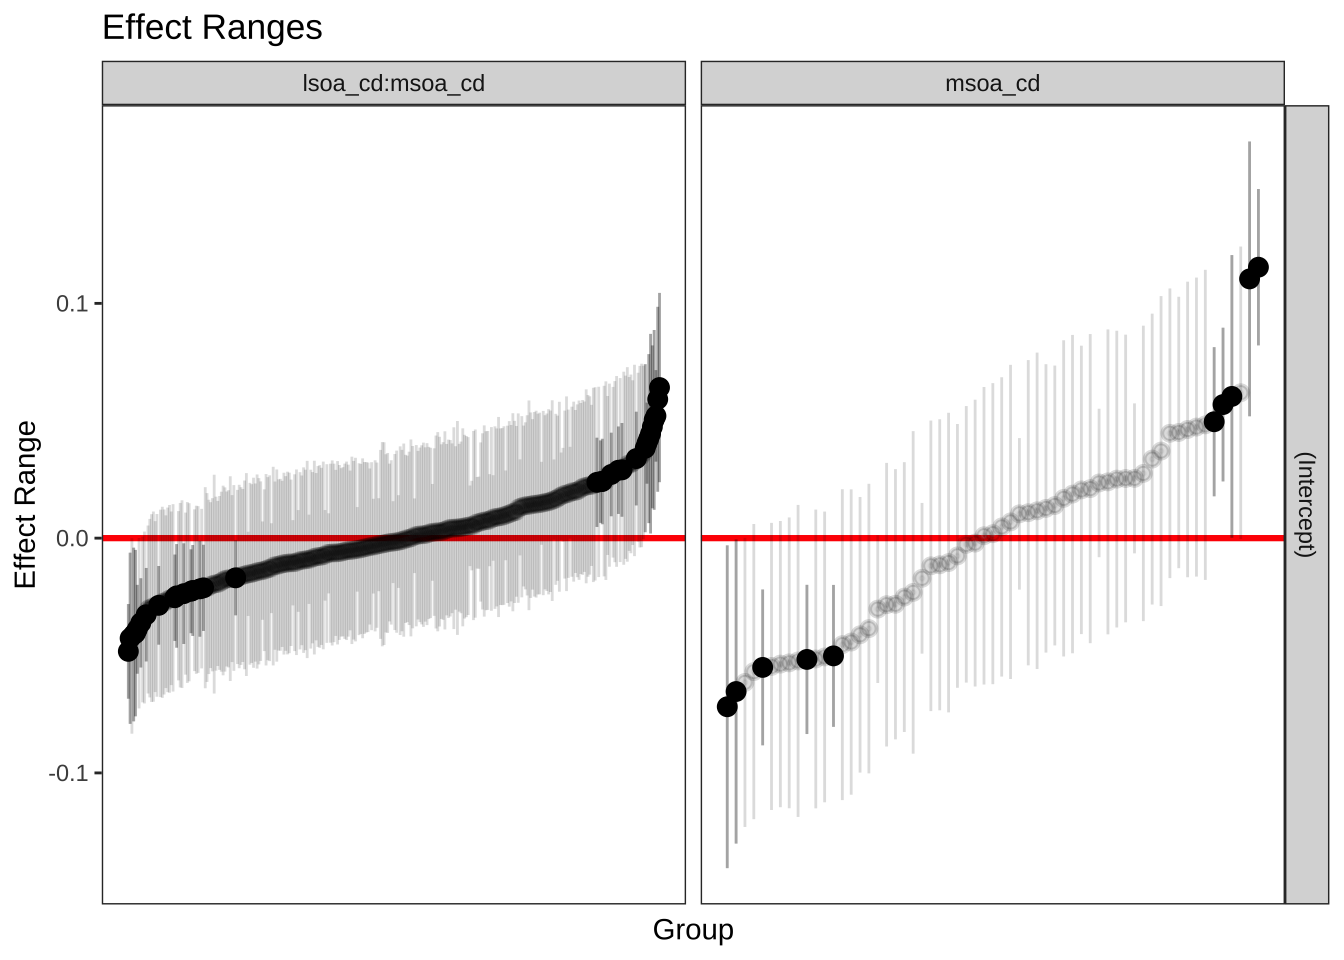
\includegraphics{07-multilevel-01_files/figure-pdf/unnamed-chunk-21-1.pdf}

Focusing on the plot on the right, we see MSOAs whose mean proportion of
unemployed population, assuming no explanatory variables, is lower than
average. These are the dots below the horizontal red line. On the
right-hand side of the plot, you will see MSOAs whose mean proportion is
higher than average. The MSOAs with the smallest residuals include the
districts of Allerton and Hunt Cross, Church, Childwall, Wavertree and
Woolton.

\marginnote{\begin{footnotesize}

\begin{tcolorbox}[enhanced jigsaw, colframe=quarto-callout-tip-color-frame, leftrule=.75mm, arc=.35mm, breakable, opacityback=0, bottomrule=.15mm, colback=white, rightrule=.15mm, toprule=.15mm, left=2mm]

\textbf{Task} What districts do we have at the other extreme? Have a go
at identifying them.

\end{tcolorbox}

\end{footnotesize}}

\begin{Shaded}
\begin{Highlighting}[]
\NormalTok{re }\OtherTok{\textless{}{-}} \FunctionTok{REsim}\NormalTok{(model3)}
\NormalTok{oa\_shp }\SpecialCharTok{\%\textgreater{}\%}\NormalTok{ dplyr}\SpecialCharTok{::}\FunctionTok{select}\NormalTok{(msoa\_cd, ward\_nm, unemp) }\SpecialCharTok{\%\textgreater{}\%}
    \FunctionTok{filter}\NormalTok{(}\FunctionTok{as.character}\NormalTok{(msoa\_cd) }\SpecialCharTok{==} \StringTok{"E02001387"} \SpecialCharTok{|} \FunctionTok{as.character}\NormalTok{(msoa\_cd) }\SpecialCharTok{==} \StringTok{"E02001393"}\NormalTok{)}
\end{Highlighting}
\end{Shaded}

\begin{verbatim}
Simple feature collection with 49 features and 3 fields
Geometry type: POLYGON
Dimension:     XY
Bounding box:  xmin: 339178.6 ymin: 386244.2 xmax: 341959.9 ymax: 389646.7
Projected CRS: Transverse_Mercator
First 10 features:
     msoa_cd                  ward_nm      unemp                       geometry
1  E02001393 Allerton and Hunts Cross 0.03246753 POLYGON ((341333.6 387163.2...
2  E02001393 Allerton and Hunts Cross 0.03684211 POLYGON ((340658.2 387205.6...
3  E02001393                   Church 0.04098361 POLYGON ((339908.1 387222.3...
4  E02001393 Allerton and Hunts Cross 0.05982906 POLYGON ((340306 386587, 34...
5  E02001393                   Church 0.01212121 POLYGON ((339974.2 387118.5...
6  E02001393                   Church 0.09219858 POLYGON ((340181.4 386957.8...
7  E02001393                   Church 0.01986755 POLYGON ((340301.2 386582.2...
8  E02001393                   Church 0.04615385 POLYGON ((340375.9 386918.6...
9  E02001393 Allerton and Hunts Cross 0.04117647 POLYGON ((340435.3 386337.4...
10 E02001393 Allerton and Hunts Cross 0.02272727 POLYGON ((340681.7 386614.4...
\end{verbatim}

We can also map the MSOA-level \emph{random effects}. To this end, we
first need to read a shapefile containing data at the MSOA level and
merge it with the \emph{random effects} estimates.

\begin{Shaded}
\begin{Highlighting}[]
\CommentTok{\# read data}
\NormalTok{msoa\_shp }\OtherTok{\textless{}{-}} \FunctionTok{st\_read}\NormalTok{(}\StringTok{"data/mlm/MSOA.shp"}\NormalTok{)}
\end{Highlighting}
\end{Shaded}

\begin{verbatim}
Reading layer `MSOA' from data source 
  `/Users/franciscorowe/Dropbox/Francisco/uol/teaching/envs453/202324/san/data/mlm/MSOA.shp' 
  using driver `ESRI Shapefile'
Simple feature collection with 61 features and 17 fields
Geometry type: MULTIPOLYGON
Dimension:     XY
Bounding box:  xmin: 333086.1 ymin: 381426.3 xmax: 345636 ymax: 397980.1
Projected CRS: Transverse_Mercator
\end{verbatim}

\begin{Shaded}
\begin{Highlighting}[]
\CommentTok{\# create a dataframe for MSOA{-}level random effects}
\NormalTok{re\_msoa }\OtherTok{\textless{}{-}}\NormalTok{ re }\SpecialCharTok{\%\textgreater{}\%} \FunctionTok{filter}\NormalTok{(groupFctr }\SpecialCharTok{==} \StringTok{"msoa\_cd"}\NormalTok{)}
\FunctionTok{str}\NormalTok{(re\_msoa)}
\end{Highlighting}
\end{Shaded}

\begin{verbatim}
'data.frame':   61 obs. of  6 variables:
 $ groupFctr: chr  "msoa_cd" "msoa_cd" "msoa_cd" "msoa_cd" ...
 $ groupID  : chr  "E02001347" "E02001348" "E02001349" "E02001350" ...
 $ term     : chr  "(Intercept)" "(Intercept)" "(Intercept)" "(Intercept)" ...
 $ mean     : num  -0.00897 -0.02846 -0.02772 0.00339 0.02241 ...
 $ median   : num  -0.0107 -0.0277 -0.0289 0.0016 0.0208 ...
 $ sd       : num  0.0336 0.0304 0.0311 0.0301 0.016 ...
\end{verbatim}

\begin{Shaded}
\begin{Highlighting}[]
\CommentTok{\# merge data}
\NormalTok{msoa\_shp }\OtherTok{\textless{}{-}} \FunctionTok{merge}\NormalTok{(}\AttributeTok{x =}\NormalTok{ msoa\_shp, }\AttributeTok{y =}\NormalTok{ re\_msoa, }\AttributeTok{by.x =} \StringTok{"MSOA\_CD"}\NormalTok{, }\AttributeTok{by.y =} \StringTok{"groupID"}\NormalTok{)}
\end{Highlighting}
\end{Shaded}

Now we can create our map:

\begin{Shaded}
\begin{Highlighting}[]
\CommentTok{\# ensure geometry is valid}
\NormalTok{msoa\_shp }\OtherTok{=}\NormalTok{ sf}\SpecialCharTok{::}\FunctionTok{st\_make\_valid}\NormalTok{(msoa\_shp)}

\CommentTok{\# create a map}
\NormalTok{legend\_title }\OtherTok{=} \FunctionTok{expression}\NormalTok{(}\StringTok{"MSOA{-}level residuals"}\NormalTok{)}
\NormalTok{map\_msoa }\OtherTok{=} \FunctionTok{tm\_shape}\NormalTok{(msoa\_shp) }\SpecialCharTok{+}
  \FunctionTok{tm\_fill}\NormalTok{(}\AttributeTok{col =} \StringTok{"mean"}\NormalTok{, }\AttributeTok{title =}\NormalTok{ legend\_title, }\AttributeTok{palette =} \FunctionTok{magma}\NormalTok{(}\DecValTok{256}\NormalTok{, }\AttributeTok{begin =} \DecValTok{0}\NormalTok{, }\AttributeTok{end =} \DecValTok{1}\NormalTok{), }\AttributeTok{style =} \StringTok{"cont"}\NormalTok{) }\SpecialCharTok{+} 
  \FunctionTok{tm\_borders}\NormalTok{(}\AttributeTok{col =} \StringTok{"white"}\NormalTok{, }\AttributeTok{lwd =}\NormalTok{ .}\DecValTok{01}\NormalTok{)  }\SpecialCharTok{+} 
  \FunctionTok{tm\_compass}\NormalTok{(}\AttributeTok{type =} \StringTok{"arrow"}\NormalTok{, }\AttributeTok{position =} \FunctionTok{c}\NormalTok{(}\StringTok{"right"}\NormalTok{, }\StringTok{"top"}\NormalTok{) , }\AttributeTok{size =} \DecValTok{4}\NormalTok{) }\SpecialCharTok{+} 
  \FunctionTok{tm\_scale\_bar}\NormalTok{(}\AttributeTok{breaks =} \FunctionTok{c}\NormalTok{(}\DecValTok{0}\NormalTok{,}\DecValTok{1}\NormalTok{,}\DecValTok{2}\NormalTok{), }\AttributeTok{text.size =} \FloatTok{0.5}\NormalTok{, }\AttributeTok{position =}  \FunctionTok{c}\NormalTok{(}\StringTok{"center"}\NormalTok{, }\StringTok{"bottom"}\NormalTok{)) }
\NormalTok{map\_msoa}
\end{Highlighting}
\end{Shaded}

\includegraphics{07-multilevel-01_files/figure-pdf/unnamed-chunk-24-1.pdf}

\subsection{Adding Individual-level Predictors}\label{sec-indlevel}

In this example, \(\mu\) represents the sample mean but it could include
a collection of independent variables or predictors. To explain the
logic, we will assume that unemployment is strongly associated to
long-term illness. We could expect that long-term illness
(\texttt{lt\_ill}) will reduce the chances of working and therefore
being unemployed. Note that our focus is on the relationship, not on
establishing causation. Specifically we want to estimate the
relationship between unemployment and long-term illness and we are
interested in variations in OA-level unemployment by MSOAs so we will
estimate the following two-level model:

OA-level:

\[y_{ij} = \beta_{0j} + \beta_{1}x_{ij} + e_{ij}\] MSOA-level:

\[\beta_{0j} = \beta_{0} + u_{0j}\] Replacing the first equation into
the second, we have:

\[y_{ij} = (\beta_{0} + u_{0j}) + \beta_{1}x_{ij} + e_{ij}\] where \(y\)
the proportion of unemployed population in OA \(i\) within MSOA \(j\);
\(\beta_{0}\) is the fixed intercept (averaging over all MSOAs);
\(u_{0j}\) represents the MSOA-level residuals or \emph{random effects};
\(\beta_{0}\) and \(u_{0j}\) together represent the varying-intercept;
\(\beta_{1}\) is the slope coefficient; \(x_{ij}\) represents the
percentage of long-term illness population; and, \(e_{ij}\) is the
individual-level residuals.

We estimate the model executing:

\begin{Shaded}
\begin{Highlighting}[]
\CommentTok{\# change to proportion}
\NormalTok{oa\_shp}\SpecialCharTok{$}\NormalTok{lt\_ill }\OtherTok{\textless{}{-}}\NormalTok{ lt\_ill}\SpecialCharTok{/}\DecValTok{100}

\CommentTok{\# specify a model equation}
\NormalTok{eq4 }\OtherTok{\textless{}{-}}\NormalTok{ unemp }\SpecialCharTok{\textasciitilde{}}\NormalTok{ lt\_ill }\SpecialCharTok{+}\NormalTok{ (}\DecValTok{1} \SpecialCharTok{|}\NormalTok{ msoa\_cd)}
\NormalTok{model4 }\OtherTok{\textless{}{-}} \FunctionTok{lmer}\NormalTok{(eq4, }\AttributeTok{data =}\NormalTok{ oa\_shp)}

\CommentTok{\# estimates}
\FunctionTok{summary}\NormalTok{(model4)}
\end{Highlighting}
\end{Shaded}

\begin{verbatim}
Linear mixed model fit by REML ['lmerMod']
Formula: unemp ~ lt_ill + (1 | msoa_cd)
   Data: oa_shp

REML criterion at convergence: -4711.9

Scaled residuals: 
    Min      1Q  Median      3Q     Max 
-5.1941 -0.5718 -0.0906  0.4507  5.9393 

Random effects:
 Groups   Name        Variance Std.Dev.
 msoa_cd  (Intercept) 0.001421 0.03769 
 Residual             0.002674 0.05171 
Number of obs: 1584, groups:  msoa_cd, 61

Fixed effects:
            Estimate Std. Error t value
(Intercept)  0.04682    0.00625   7.492
lt_ill       0.29588    0.01615  18.317

Correlation of Fixed Effects:
       (Intr)
lt_ill -0.600
\end{verbatim}

\emph{Fixed effects}: model averaging over MSOAs

\begin{Shaded}
\begin{Highlighting}[]
\FunctionTok{fixef}\NormalTok{(model4)}
\end{Highlighting}
\end{Shaded}

\begin{verbatim}
(Intercept)      lt_ill 
 0.04681959  0.29588110 
\end{verbatim}

yields an estimated regression line in an average McSOA:
\(y = 0.04681959 + 0.29588110x\)

\emph{Random effects}: MSOA-level errors

\begin{Shaded}
\begin{Highlighting}[]
\NormalTok{ranef\_m4 }\OtherTok{\textless{}{-}} \FunctionTok{ranef}\NormalTok{(model4)}
\FunctionTok{head}\NormalTok{(ranef\_m4}\SpecialCharTok{$}\NormalTok{msoa\_cd, }\DecValTok{5}\NormalTok{)}
\end{Highlighting}
\end{Shaded}

\begin{verbatim}
           (Intercept)
E02001347 -0.017474815
E02001348 -0.021203807
E02001349 -0.022469313
E02001350 -0.003539869
E02001351  0.008502813
\end{verbatim}

yields an estimated intercept for MSOA \texttt{E02001347} which is
\texttt{0.017474815} lower than the average with a regression line:
\texttt{(0.04681959\ -\ 0.017474815)\ +\ 0.29588110x} \texttt{=}
\texttt{0.02934478\ +\ 0.29588110x}. You can confirm this by looking at
the estimated model within each MSOA by executing on the first row:

\begin{Shaded}
\begin{Highlighting}[]
\FunctionTok{coef}\NormalTok{(model4) }\SpecialCharTok{\%\textgreater{}\%} \FunctionTok{head}\NormalTok{(}\AttributeTok{n =} \DecValTok{5}\NormalTok{ )}
\end{Highlighting}
\end{Shaded}

\begin{verbatim}
$msoa_cd
            (Intercept)    lt_ill
E02001347  0.0293447796 0.2958811
E02001348  0.0256157871 0.2958811
E02001349  0.0243502820 0.2958811
E02001350  0.0432797257 0.2958811
E02001351  0.0553224074 0.2958811
E02001352  0.0636246817 0.2958811
E02001353  0.0160357811 0.2958811
E02001354  0.0581675090 0.2958811
E02001355  0.0528556223 0.2958811
E02001356  0.1061228409 0.2958811
E02001357  0.0582394764 0.2958811
E02001358  0.0740589539 0.2958811
E02001359  0.0174543833 0.2958811
E02001360  0.0715947302 0.2958811
E02001361  0.0466345080 0.2958811
E02001362  0.0160157652 0.2958811
E02001363  0.0815677365 0.2958811
E02001364  0.0934291622 0.2958811
E02001365  0.0919597741 0.2958811
E02001366  0.0620614209 0.2958811
E02001367  0.0030188157 0.2958811
E02001368  0.0808079877 0.2958811
E02001369  0.0632672806 0.2958811
E02001370  0.1335873521 0.2958811
E02001371  0.0515952786 0.2958811
E02001372  0.0309188138 0.2958811
E02001373  0.0545884863 0.2958811
E02001374  0.1039777893 0.2958811
E02001375  0.0409780838 0.2958811
E02001376  0.0964558147 0.2958811
E02001377  0.0558567086 0.2958811
E02001378  0.0241577873 0.2958811
E02001380  0.0046345234 0.2958811
E02001381  0.0711500934 0.2958811
E02001382  0.0064505905 0.2958811
E02001383  0.0742504417 0.2958811
E02001384  0.0490214750 0.2958811
E02001385  0.1707802796 0.2958811
E02001386  0.0336177791 0.2958811
E02001387 -0.0007218010 0.2958811
E02001388  0.0125049014 0.2958811
E02001389  0.0711118539 0.2958811
E02001390  0.0805482208 0.2958811
E02001391  0.0417458225 0.2958811
E02001392 -0.0074952916 0.2958811
E02001393 -0.0051402516 0.2958811
E02001394  0.0181501721 0.2958811
E02001395  0.0009387908 0.2958811
E02001396  0.0521380692 0.2958811
E02001397 -0.0006698249 0.2958811
E02001398  0.0197886833 0.2958811
E02001399  0.0030131040 0.2958811
E02001400  0.0274024412 0.2958811
E02001401 -0.0043446188 0.2958811
E02001402  0.0074558647 0.2958811
E02001403  0.0539235547 0.2958811
E02001404  0.0647550886 0.2958811
E02001405  0.0903509760 0.2958811
E02006932  0.0310245337 0.2958811
E02006933  0.0276019142 0.2958811
E02006934  0.0350623557 0.2958811
\end{verbatim}

\emph{Fixed effect correlations}

In the bottom of the output, we have the correlations between the
fixed-effects estimates. In our example, it refers to the correlation
between \(\beta_{0}\) and \(\beta_{1}\). It is negative indicating that
in MSOAs where the relationship between unemployment and long-term
illness is greater, as measured by \(\beta_{1}\), the average proportion
of unemployed people tends to be smaller, as captured by \(\beta_{0}\).

\subsection{Adding Group-level Predictors}\label{sec-grouplevel}

We can also add group-level predictors. We use the formulation:

OA-level:

\[y_{ij} = \beta_{0j} + \beta_{1}x_{ij} + e_{ij}\]

MSOA-level:

\[\beta_{0j} = \beta_{0} + \gamma_{1}m_{j} + u_{0j}\]

where \(x_{ij}\) is the OA-level proportion of population suffering
long-term illness and \(m_{j}\) is the MSOA-level proportion of male
population. We first need to create this group-level predictor:

\begin{Shaded}
\begin{Highlighting}[]
\CommentTok{\# detach OA shp and attach MSOA shp}
\FunctionTok{detach}\NormalTok{(oa\_shp)}
\FunctionTok{attach}\NormalTok{(msoa\_shp)}

\CommentTok{\# group{-}level predictor}
\NormalTok{msoa\_shp}\SpecialCharTok{$}\NormalTok{pr\_male }\OtherTok{\textless{}{-}}\NormalTok{ males}\SpecialCharTok{/}\NormalTok{pop}

\CommentTok{\# remove geometries}
\NormalTok{msoa\_df }\OtherTok{\textless{}{-}} \StringTok{\textasciigrave{}}\AttributeTok{st\_geometry\textless{}{-}}\StringTok{\textasciigrave{}}\NormalTok{(msoa\_shp, }\ConstantTok{NULL}\NormalTok{)}

\CommentTok{\# select variables}
\NormalTok{msoa\_df }\OtherTok{\textless{}{-}}\NormalTok{ msoa\_df }\SpecialCharTok{\%\textgreater{}\%}\NormalTok{ dplyr}\SpecialCharTok{::}\FunctionTok{select}\NormalTok{(MSOA\_CD, pop, pr\_male)}

\CommentTok{\# merge data sets}
\NormalTok{oa\_shp }\OtherTok{\textless{}{-}} \FunctionTok{merge}\NormalTok{(}\AttributeTok{x=}\NormalTok{oa\_shp, }\AttributeTok{y=}\NormalTok{msoa\_df, }\AttributeTok{by.x =} \StringTok{"msoa\_cd"}\NormalTok{, }\AttributeTok{by.y=}\StringTok{"MSOA\_CD"}\NormalTok{)}

\CommentTok{\# inspect data}
\FunctionTok{head}\NormalTok{(oa\_shp[}\DecValTok{1}\SpecialCharTok{:}\DecValTok{10}\NormalTok{, }\FunctionTok{c}\NormalTok{(}\StringTok{"msoa\_cd"}\NormalTok{, }\StringTok{"oa\_cd"}\NormalTok{, }\StringTok{"unemp"}\NormalTok{, }\StringTok{"pr\_male"}\NormalTok{)])}
\end{Highlighting}
\end{Shaded}

\begin{verbatim}
Simple feature collection with 6 features and 4 fields
Geometry type: POLYGON
Dimension:     XY
Bounding box:  xmin: 337693.5 ymin: 396068.2 xmax: 339430.9 ymax: 397790
Projected CRS: Transverse_Mercator
    msoa_cd     oa_cd      unemp   pr_male                       geometry
1 E02001347 E00033730 0.10322581 0.4775905 POLYGON ((338376 397059, 33...
2 E02001347 E00033722 0.06306306 0.4775905 POLYGON ((337929.4 397669.9...
3 E02001347 E00033712 0.09090909 0.4775905 POLYGON ((338830 396068.2, ...
4 E02001347 E00033739 0.09401709 0.4775905 POLYGON ((339140.3 397191, ...
5 E02001347 E00033719 0.05855856 0.4775905 POLYGON ((338128.8 397658.6...
6 E02001347 E00033711 0.12195122 0.4775905 POLYGON ((339163.2 396833.6...
\end{verbatim}

We can now estimate our model:

\begin{Shaded}
\begin{Highlighting}[]
\FunctionTok{detach}\NormalTok{(msoa\_shp)}
\FunctionTok{attach}\NormalTok{(oa\_shp)}

\CommentTok{\# specify a model equation}
\NormalTok{eq5 }\OtherTok{\textless{}{-}}\NormalTok{ unemp }\SpecialCharTok{\textasciitilde{}}\NormalTok{ lt\_ill }\SpecialCharTok{+}\NormalTok{ pr\_male }\SpecialCharTok{+}\NormalTok{ (}\DecValTok{1} \SpecialCharTok{|}\NormalTok{ msoa\_cd)}
\NormalTok{model5 }\OtherTok{\textless{}{-}} \FunctionTok{lmer}\NormalTok{(eq5, }\AttributeTok{data =}\NormalTok{ oa\_shp)}

\CommentTok{\# estimates}
\FunctionTok{summary}\NormalTok{(model5)}
\end{Highlighting}
\end{Shaded}

\begin{verbatim}
Linear mixed model fit by REML ['lmerMod']
Formula: unemp ~ lt_ill + pr_male + (1 | msoa_cd)
   Data: oa_shp

REML criterion at convergence: -4712.3

Scaled residuals: 
    Min      1Q  Median      3Q     Max 
-5.2162 -0.5696 -0.0929  0.4549  5.9370 

Random effects:
 Groups   Name        Variance Std.Dev.
 msoa_cd  (Intercept) 0.001391 0.03729 
 Residual             0.002674 0.05171 
Number of obs: 1584, groups:  msoa_cd, 61

Fixed effects:
            Estimate Std. Error t value
(Intercept) -0.07746    0.08768  -0.883
lt_ill       0.29781    0.01620  18.389
pr_male      0.25059    0.17642   1.420

Correlation of Fixed Effects:
        (Intr) lt_ill
lt_ill  -0.118       
pr_male -0.997  0.075
\end{verbatim}

This model includes the proportion of males and intercepts that vary by
MSOA. The \texttt{lmer()} function only accepts predictors at the
individual level, so we have included data on the proportion of male
population at this level. Explore and interpret the model running the
functions below:

\begin{Shaded}
\begin{Highlighting}[]
\CommentTok{\# fixed effects}
\FunctionTok{fixef}\NormalTok{(model5)}
\end{Highlighting}
\end{Shaded}

\begin{verbatim}
(Intercept)      lt_ill     pr_male 
 -0.0774607   0.2978084   0.2505913 
\end{verbatim}

\begin{Shaded}
\begin{Highlighting}[]
\CommentTok{\# random effects}
\NormalTok{ranef\_m5 }\OtherTok{\textless{}{-}} \FunctionTok{ranef}\NormalTok{(model5)}
\FunctionTok{head}\NormalTok{(ranef\_m5}\SpecialCharTok{$}\NormalTok{msoa\_cd, }\DecValTok{5}\NormalTok{)}
\end{Highlighting}
\end{Shaded}

\begin{verbatim}
           (Intercept)
E02001347 -0.013625261
E02001348 -0.019757846
E02001349 -0.023709992
E02001350  0.003003861
E02001351  0.003508477
\end{verbatim}

Adding group-level predictors tends to improve inferences for group
coefficients. Examine the confidence intervals, in order to evalute how
the precision of our estimates of the MSOA intercepts have changed.
\emph{Have confidence intervals for the intercepts of Model 4 and 5
increased or reduced?} Hint: look at how to get the confidence intervals
above.

\section{Questions}\label{questions-3}

For the second assignment, we will be using a different dataset
comprising information on COVID-19 cases, census data and the Index of
Multiple Deprivation (IMD) for England. The data set is similar in
structured to that used in this chapter. It is hierarchically organised
into 149 Upper Tier Local Authority Districts (UTLADs) within 9 Regions
and has 508 variables - see Chapter @ref(datasets) for a more detailed
description of the data.

\begin{Shaded}
\begin{Highlighting}[]
\NormalTok{sdf }\OtherTok{\textless{}{-}} \FunctionTok{st\_read}\NormalTok{(}\StringTok{"data/assignment\_2\_covid/covid19\_eng.gpkg"}\NormalTok{)}
\end{Highlighting}
\end{Shaded}

\begin{verbatim}
Reading layer `covid19_eng' from data source 
  `/Users/franciscorowe/Dropbox/Francisco/uol/teaching/envs453/202324/san/data/assignment_2_covid/covid19_eng.gpkg' 
  using driver `GPKG'
Simple feature collection with 149 features and 507 fields
Geometry type: MULTIPOLYGON
Dimension:     XY
Bounding box:  xmin: 134112.4 ymin: 11429.67 xmax: 655653.8 ymax: 657536
Projected CRS: OSGB36 / British National Grid
\end{verbatim}

Here we see a selection of 10 variables for 5 UTLADs.

\begin{Shaded}
\begin{Highlighting}[]
\FunctionTok{head}\NormalTok{(sdf[}\DecValTok{1}\SpecialCharTok{:}\DecValTok{5}\NormalTok{,}\FunctionTok{c}\NormalTok{(}\DecValTok{3}\NormalTok{,}\DecValTok{4}\NormalTok{,}\DecValTok{9}\NormalTok{,}\DecValTok{10}\NormalTok{,}\DecValTok{381}\NormalTok{,}\DecValTok{385}\NormalTok{,}\DecValTok{386}\NormalTok{,}\DecValTok{387}\NormalTok{,}\DecValTok{403}\NormalTok{,}\DecValTok{406}\NormalTok{)])}
\end{Highlighting}
\end{Shaded}

\begin{verbatim}
Simple feature collection with 5 features and 10 fields
Geometry type: MULTIPOLYGON
Dimension:     XY
Bounding box:  xmin: 418871.2 ymin: 506329.3 xmax: 478441.5 ymax: 537152
Projected CRS: OSGB36 / British National Grid
             ctyua19nm     Region X2020.01.31 X2020.02.01 IMD...Average.score
1           Hartlepool North East           0           0              35.037
2        Middlesbrough North East           0           0              40.460
3 Redcar and Cleveland North East           0           0              29.792
4     Stockton-on-Tees North East           0           0              25.790
5           Darlington North East           0           0              25.657
  Residents Households Dwellings Age_85plus White_British_and_Irish
1     92028      40434     42102       1856                   89117
2    138412      57203     59956       2465                  119680
3    135177      59605     61899       3113                  132343
4    191610      79159     82237       3481                  179501
5    105564      46670     48644       2550                   99226
                            geom
1 MULTIPOLYGON (((447097 5371...
2 MULTIPOLYGON (((449862.8 52...
3 MULTIPOLYGON (((455939.7 52...
4 MULTIPOLYGON (((444126.1 52...
5 MULTIPOLYGON (((423475.7 52...
\end{verbatim}

\begin{itemize}
\tightlist
\item
  \texttt{ctyua19nm}: Upper Tier Local Authority District name
\item
  \texttt{Region}: Region name
\item
  \texttt{X2020.01.31}: COVID-19 cases on January 31st 2020
\item
  \texttt{X2020.02.01}: COVID-19 cases on February 1st 2020
\item
  \texttt{IMD...Average.score}: Average IMD score for UTLADs - see
  \href{https://www.gov.uk/government/statistics/english-indices-of-deprivation-2019}{File
  11: upper-tier local authority summaries} for information on this and
  associated indicators.
\item
  \texttt{Residents}: Number of residents
\item
  \texttt{Households}: Number of households
\item
  \texttt{Dwellings}: Number of dwellings
\item
  \texttt{Age\_85plus}: Number of people aged 85 and over
\item
  \texttt{White\_British\_and\_Irish}: Number of white British and Irish
  people
\end{itemize}

Note that variable names relating to the daily COVID-19 cases are
organised in the following way: \texttt{X} stands for daily COVID-19
cases, followed by the year (i.e.~2020, 2021); month (i.e.~January to
December); and day (i.e.~01 to 31).

Using these data, you are required to address the following challenges:

\begin{enumerate}
\def\labelenumi{\arabic{enumi}.}
\item
  Fit a varying-intercept model with no explanatory variables. Let the
  intercept to vary by region.
\item
  Fit a varying-intercept model with including at least three
  explanatory variables.
\item
  Compute the Variance Partition Coefficient (VPC) for the models
  estimated according to points 1 and 2 above.
\item
  Create caterpillar plots to visualise the varying intercepts.
\end{enumerate}

Analyse and discuss: 1. the extent of variation in the dependent
variables at the two geographical scales (variation at which
geographical scale explains most of variance in your dependent
variable); 2. the varying intercept estimate(s) from your model(s) (what
can they tell you about the difference between groups / areas? are they
statistically significantly different?);

Ensure you appropriately describe the structure of the data and identify
the various geographical scales of analysis (i.e.~level-1 and level-2
units)

In addressing the challenges in this and following chapters, you have
some flexibility to be creative. A set of key factors to consider:

\begin{enumerate}
\def\labelenumi{\arabic{enumi}.}
\tightlist
\item
  \emph{Dependent Variable}: We will seek to explain daily COVID-19
  cases, and you will need to make a decision as to:
\end{enumerate}

\begin{itemize}
\item
  \emph{Daily vs cumulative COVID-19 cases}. Given that we will be
  focusing on cross-sectional models (i.e.~models for one snapshot), you
  can focus on modelling daily cases at one specific date or cumulative
  daily cases over a period of time.
\item
  \emph{Time period}. You can select the date or period of time that you
  will focus your analysis on.
\item
  \emph{Use risk of COVID-19 infection}. The dependent variable should
  be the risk or rate of COVID-19 infection.
\end{itemize}

For example, the risk of COVID-19 infection for the period (i.e.~between
Dec.~1st, 2020 - January 29th, 2021) comprising the third wave of the
pandemic in the United Kingdom can be computed as:

\begin{Shaded}
\begin{Highlighting}[]
\CommentTok{\# computing cumulative COVID cases for  01/12/2020 {-} 29/01/2021}
\NormalTok{sdf[, }\DecValTok{509}\NormalTok{] }\OtherTok{\textless{}{-}}\NormalTok{ sdf }\SpecialCharTok{\%\textgreater{}\%}\NormalTok{ dplyr}\SpecialCharTok{::}\FunctionTok{select}\NormalTok{(}\StringTok{"X2020.12.01"}\SpecialCharTok{:}\StringTok{"X2021.01.29"}\NormalTok{) }\SpecialCharTok{\%\textgreater{}\%} \CommentTok{\# select COVID cases 01/12/2020 {-} 29/01/2021}
  \FunctionTok{mutate}\NormalTok{(}\AttributeTok{cum\_covid =} \FunctionTok{rowSums}\NormalTok{(}\FunctionTok{across}\NormalTok{(}\FunctionTok{where}\NormalTok{(is.numeric)))) }\SpecialCharTok{\%\textgreater{}\%} \CommentTok{\# sum daily cases}
\NormalTok{  dplyr}\SpecialCharTok{::}\FunctionTok{select}\NormalTok{(cum\_covid) }\SpecialCharTok{\%\textgreater{}\%} \CommentTok{\# select cumulative cases}
   \FunctionTok{st\_set\_geometry}\NormalTok{(., }\ConstantTok{NULL}\NormalTok{) }\CommentTok{\# set geometry to NULL}

\CommentTok{\# computing risk of infection}
\NormalTok{sdf }\OtherTok{\textless{}{-}}\NormalTok{ sdf }\SpecialCharTok{\%\textgreater{}\%}  \FunctionTok{mutate}\NormalTok{(}
  \AttributeTok{covid19\_r =} \FunctionTok{round}\NormalTok{((cum\_covid }\SpecialCharTok{/}\NormalTok{ Residents ) }\SpecialCharTok{*} \DecValTok{1000}\NormalTok{) }
\NormalTok{  )}
\end{Highlighting}
\end{Shaded}

\begin{enumerate}
\def\labelenumi{\arabic{enumi}.}
\setcounter{enumi}{1}
\tightlist
\item
  \emph{Explanatory variables}:
\end{enumerate}

\begin{itemize}
\item
  \emph{At least 3}. Use at least 3 explanatory variables. There is no
  maximum limit but consider your model to be parsimonious.
\item
  \emph{Choice your set}. Select the set of variables you consider
  appropriate / interesting. Make sure you justify your choice based on
  evidence and/or theory.
\item
  \emph{Percentages / Proportions}. Use percentages or proportions to
  capture the composition of places, rather than numbers of people,
  households or dwellings. For this, ensure you are using the
  appropriate denominator.
\end{itemize}

For instance, if you want to capture the relationship between cumulative
COVID-19 cases and overcrowding, share of elderly population and
nonwhite minorities, use the following variables

\begin{Shaded}
\begin{Highlighting}[]
\NormalTok{sdf }\OtherTok{\textless{}{-}}\NormalTok{ sdf }\SpecialCharTok{\%\textgreater{}\%} \FunctionTok{mutate}\NormalTok{(}
  \AttributeTok{crowded\_hou =}\NormalTok{ Crowded\_housing }\SpecialCharTok{/}\NormalTok{ Households, }\CommentTok{\# share of crowded housing}
  \AttributeTok{elderly =}\NormalTok{ (Age\_85plus) }\SpecialCharTok{/}\NormalTok{ Residents, }\CommentTok{\# share of population aged 65+}
  \AttributeTok{ethnic =}\NormalTok{ (Mixed }\SpecialCharTok{+}\NormalTok{ Indian }\SpecialCharTok{+}\NormalTok{ Pakistani }\SpecialCharTok{+}\NormalTok{ Bangladeshi }\SpecialCharTok{+}\NormalTok{ Chinese }\SpecialCharTok{+}\NormalTok{ Other\_Asian }\SpecialCharTok{+}\NormalTok{ Black }\SpecialCharTok{+}\NormalTok{ Other\_ethnicity) }\SpecialCharTok{/}\NormalTok{ Residents, }\CommentTok{\# share of nonwhite population}
\NormalTok{)}
\end{Highlighting}
\end{Shaded}

\textbf{ADVICE}: Create a new spatial data frame including only the
variables you will analyse. For example:

\begin{Shaded}
\begin{Highlighting}[]
\NormalTok{nsdf }\OtherTok{\textless{}{-}}\NormalTok{ sdf  }\SpecialCharTok{\%\textgreater{}\%}\NormalTok{  dplyr}\SpecialCharTok{::}\FunctionTok{select}\NormalTok{(objectid, }
\NormalTok{                         ctyua19cd, }
\NormalTok{                         ctyua19nm, }
\NormalTok{                         Region, }
\NormalTok{                         covid19\_r, }
\NormalTok{                         crowded\_hou, }
\NormalTok{                         elderly, }
\NormalTok{                         ethnic, }
\NormalTok{                         Residents)}
\end{Highlighting}
\end{Shaded}

\bookmarksetup{startatroot}

\chapter{Multilevel Modelling - Part 2}\label{sec-chp8}

This chapter explains varying slopes and draws on the following
references:

The content of this chapter is based on:

\begin{itemize}
\item
  Gelman and Hill (2006) provides an excellent and intuitive explanation
  of multilevel modelling and data analysis in general. Read Part 2A for
  a really good explanation of multilevel models.
\item
  Multilevel Modelling (n.d.) is an useful online resource on multilevel
  modelling and is free!
\end{itemize}

\section{Dependencies}\label{dependencies-5}

This chapter uses the following libraries which are listed in the
Section~\ref{sec-dependencies} in Chapter 1:

\begin{Shaded}
\begin{Highlighting}[]
\CommentTok{\# Data manipulation, transformation and visualisation}
\FunctionTok{library}\NormalTok{(tidyverse)}
\CommentTok{\# Nice tables}
\FunctionTok{library}\NormalTok{(kableExtra)}
\CommentTok{\# Simple features (a standardised way to encode vector data ie. points, lines, polygons)}
\FunctionTok{library}\NormalTok{(sf) }
\CommentTok{\# Spatial objects conversion}
\FunctionTok{library}\NormalTok{(sp) }
\CommentTok{\# Thematic maps}
\FunctionTok{library}\NormalTok{(tmap) }
\CommentTok{\# Colour palettes}
\FunctionTok{library}\NormalTok{(viridis) }
\CommentTok{\# Fitting multilevel models}
\FunctionTok{library}\NormalTok{(lme4)}
\CommentTok{\# Tools for extracting information generated by lme4}
\FunctionTok{library}\NormalTok{(merTools)}
\CommentTok{\# Exportable regression tables}
\FunctionTok{library}\NormalTok{(jtools)}
\end{Highlighting}
\end{Shaded}

\section{Data}\label{data-4}

For this chapter, we will data for Liverpool from England's 2011 Census.
The original source is the
\href{https://www.nomisweb.co.uk/home/census2001.asp}{Office of National
Statistics} and the dataset comprises a number of selected variables
capturing demographic, health and socio-economic of the local resident
population at four geographic levels: Output Area (OA), Lower Super
Output Area (LSOA), Middle Super Output Area (MSOA) and Local Authority
District (LAD). The variables include population counts and percentages.
For a description of the variables, see the readme file in the mlm data
folder.\footnote{Read the file in R by executing
  \texttt{read\_tsv("data/mlm/readme.txt")} . Ensure the library
  \texttt{readr} is installed before running \texttt{read\_tsv}.}

Let us read the data:

\begin{Shaded}
\begin{Highlighting}[]
\CommentTok{\# clean workspace}
\FunctionTok{rm}\NormalTok{(}\AttributeTok{list=}\FunctionTok{ls}\NormalTok{())}
\CommentTok{\# read data}
\NormalTok{oa\_shp }\OtherTok{\textless{}{-}} \FunctionTok{st\_read}\NormalTok{(}\StringTok{"data/mlm/OA.shp"}\NormalTok{)}
\end{Highlighting}
\end{Shaded}

\section{Conceptual Overview}\label{conceptual-overview}

So far, we have estimated varying-intercept models; that is, when the
intercept (\(\beta_{0}\)) is allowed to vary by group (eg. geographical
area) - as shown in Fig. 1(a). The strength of the relationship between
\(y\) (i.e.~unemployment rate) and \(x\) (long-term illness) has been
assumed to be the same across groups (i.e.~MSOAs), as captured by the
regression slope (\(\beta_{1}\)). Yet it can also vary by group as shown
in Fig. 1(b), or we can observe group variability for both intercepts
and slopes as represented in Fig. 1(c).

\begin{figure}[H]

{\centering 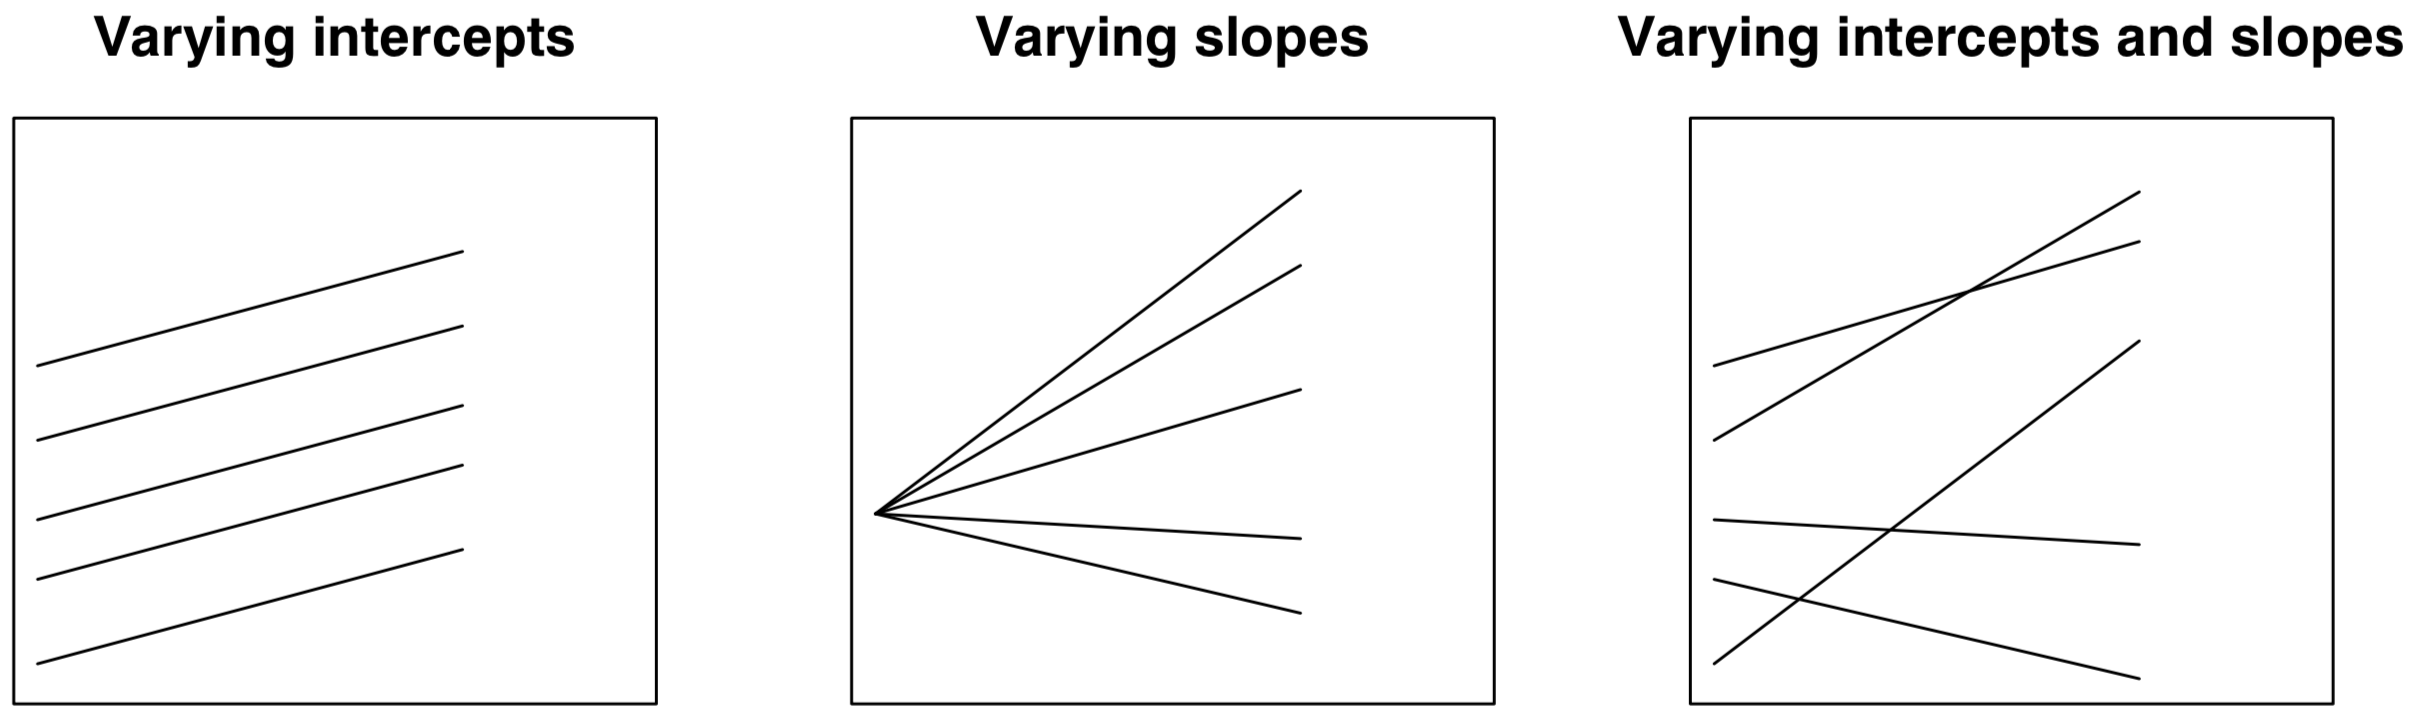
\includegraphics{figs/ch6/fig11.1_Gelman_Hill.png}

}

\caption{Fig. 1. Linear regression model with (a) varying intercepts,
(b) varying slopes, and (c) both. Source: Gelman and Hill (2006) p.238.}

\end{figure}%

\subsection{Exploratory Analysis: Varying
Slopes}\label{exploratory-analysis-varying-slopes}

Let's then explore if there is variation in the relationship between
unemployment rate and the share of population in long-term illness. We
do this by selecting the 8 MSOAs containing OAs with the highest
unemployment rates in Liverpool.

\begin{Shaded}
\begin{Highlighting}[]
\CommentTok{\# Sort data }
\NormalTok{oa\_shp }\OtherTok{\textless{}{-}}\NormalTok{ oa\_shp }\SpecialCharTok{\%\textgreater{}\%} \FunctionTok{arrange}\NormalTok{(}\SpecialCharTok{{-}}\NormalTok{unemp)}
\NormalTok{oa\_shp[}\DecValTok{1}\SpecialCharTok{:}\DecValTok{9}\NormalTok{, }\FunctionTok{c}\NormalTok{(}\StringTok{"msoa\_cd"}\NormalTok{, }\StringTok{"unemp"}\NormalTok{)]}
\end{Highlighting}
\end{Shaded}

\begin{verbatim}
Simple feature collection with 9 features and 2 fields
Geometry type: MULTIPOLYGON
Dimension:     XY
Bounding box:  xmin: 335032 ymin: 387777 xmax: 338576.1 ymax: 395022.4
Projected CRS: Transverse_Mercator
    msoa_cd     unemp                       geometry
1 E02001354 0.5000000 MULTIPOLYGON (((337491.2 39...
2 E02001369 0.4960630 MULTIPOLYGON (((335272.3 39...
3 E02001366 0.4461538 MULTIPOLYGON (((338198.1 39...
4 E02001365 0.4352941 MULTIPOLYGON (((336572.2 39...
5 E02001370 0.4024390 MULTIPOLYGON (((336328.3 39...
6 E02001390 0.3801653 MULTIPOLYGON (((335833.6 38...
7 E02001354 0.3750000 MULTIPOLYGON (((337403 3949...
8 E02001385 0.3707865 MULTIPOLYGON (((336251.6 38...
9 E02001368 0.3648649 MULTIPOLYGON (((335209.3 39...
\end{verbatim}

\begin{Shaded}
\begin{Highlighting}[]
\CommentTok{\# Select MSOAs}
\NormalTok{s\_t8 }\OtherTok{\textless{}{-}}\NormalTok{ oa\_shp }\SpecialCharTok{\%\textgreater{}\%}\NormalTok{ dplyr}\SpecialCharTok{::}\FunctionTok{filter}\NormalTok{(}
    \FunctionTok{as.character}\NormalTok{(msoa\_cd) }\SpecialCharTok{\%in\%} \FunctionTok{c}\NormalTok{(}
      \StringTok{"E02001354"}\NormalTok{, }
      \StringTok{"E02001369"}\NormalTok{, }
      \StringTok{"E02001366"}\NormalTok{, }
      \StringTok{"E02001365"}\NormalTok{, }
      \StringTok{"E02001370"}\NormalTok{, }
      \StringTok{"E02001390"}\NormalTok{, }
      \StringTok{"E02001368"}\NormalTok{, }
      \StringTok{"E02001385"}\NormalTok{)}
\NormalTok{    )}
\end{Highlighting}
\end{Shaded}

And then we generate a set of scatter plots and draw regression lines
for each MSOA.

\begin{Shaded}
\begin{Highlighting}[]
\FunctionTok{ggplot}\NormalTok{(s\_t8, }\FunctionTok{aes}\NormalTok{(}\AttributeTok{x =}\NormalTok{ lt\_ill, }\AttributeTok{y =}\NormalTok{ unemp)) }\SpecialCharTok{+} 
  \FunctionTok{geom\_point}\NormalTok{() }\SpecialCharTok{+} 
  \FunctionTok{geom\_smooth}\NormalTok{(}\AttributeTok{method =} \StringTok{"lm"}\NormalTok{) }\SpecialCharTok{+}
  \FunctionTok{facet\_wrap}\NormalTok{(}\SpecialCharTok{\textasciitilde{}}\NormalTok{ msoa\_cd, }\AttributeTok{nrow =} \DecValTok{2}\NormalTok{) }\SpecialCharTok{+}
  \FunctionTok{ylab}\NormalTok{(}\StringTok{"Unemployment rate"}\NormalTok{) }\SpecialCharTok{+} 
  \FunctionTok{xlab}\NormalTok{(}\StringTok{"Long{-}term Illness (\%)"}\NormalTok{) }\SpecialCharTok{+}
  \FunctionTok{theme\_classic}\NormalTok{()}
\end{Highlighting}
\end{Shaded}

\begin{verbatim}
`geom_smooth()` using formula = 'y ~ x'
\end{verbatim}

\includegraphics{08-multilevel-02_files/figure-pdf/unnamed-chunk-4-1.pdf}

We can observe great variability in the relationship between
unemployment rates and the percentage of population in long-term
illness. A strong and positive relationship exists in MSOA
\texttt{E02001366} (Tuebrook and Stoneycroft), while it is negative in
MSOA \texttt{E02001370} (Everton) and neutral in MSOA \texttt{E02001390}
(Princes Park \& Riverside). This visual inspection suggests that
accounting for differences in the way unmployment rates relate to
long-term illness is important. Contextual factors may differ across
MSOAs in systematic ways.

\section{Estimating Varying Intercept and Slopes
Models}\label{estimating-varying-intercept-and-slopes-models}

A way to capture for these group differences in the relationship between
unemployment rates and long-term illness is to allow the relevant slope
to vary by group (i.e.~MSOA). We can do this estimating the following
model:

OA-level:

\[y_{ij} = \beta_{0j} + \beta_{1j}x_{ij} + e_{ij}\]

MSOA-level:

\[\beta_{0j} = \beta_{0} + u_{0j}\] \[\beta_{1j} = \beta_{1} + u_{1j} \]
Replacing the first equation into the second generates:

\[y_{ij} = (\beta_{0} + u_{0j}) + (\beta_{1} + u_{1j})x_{ij} + e_{ij}\]
where, as in the previous Chapter, \(y\) the proportion of unemployed
population in OA \(i\) within MSOA \(j\); \(\beta_{0}\) is the fixed
intercept (averaging over all MSOAs); \(u_{0j}\) represents the
MSOA-level residuals, or \emph{random effects}, of the intercept;
\(e_{ij}\) is the individual-level residuals; and, \(x_{ij}\) represents
the percentage of long-term illness population. \emph{But} now we have a
varying slope represented by \(\beta_{1}\) and \(u_{1j}\): \(\beta_{1}\)
is estimated average slope - fixed part of the model; and, \(u_{1j}\) is
the estimated group-level errors of the slope.

To estimate such model, we add \texttt{lt\_ill} in the bracket with a
\texttt{+} sign between \texttt{1} and \texttt{\textbar{}}
i.e.~\texttt{(1\ +\ lt\_ill\ \textbar{}\ msoa\_cd)}.

\begin{Shaded}
\begin{Highlighting}[]
\CommentTok{\# attach df}
\FunctionTok{attach}\NormalTok{(oa\_shp)}

\CommentTok{\# change to proportion}
\NormalTok{oa\_shp}\SpecialCharTok{$}\NormalTok{lt\_ill }\OtherTok{\textless{}{-}}\NormalTok{ lt\_ill}\SpecialCharTok{/}\DecValTok{100}

\CommentTok{\# specify a model equation}
\NormalTok{eq6 }\OtherTok{\textless{}{-}}\NormalTok{ unemp }\SpecialCharTok{\textasciitilde{}}\NormalTok{ lt\_ill }\SpecialCharTok{+}\NormalTok{ (}\DecValTok{1} \SpecialCharTok{+}\NormalTok{ lt\_ill }\SpecialCharTok{|}\NormalTok{ msoa\_cd)}
\NormalTok{model6 }\OtherTok{\textless{}{-}} \FunctionTok{lmer}\NormalTok{(eq6, }\AttributeTok{data =}\NormalTok{ oa\_shp)}

\CommentTok{\# estimates}
\FunctionTok{summary}\NormalTok{(model6)}
\end{Highlighting}
\end{Shaded}

\begin{verbatim}
Linear mixed model fit by REML ['lmerMod']
Formula: unemp ~ lt_ill + (1 + lt_ill | msoa_cd)
   Data: oa_shp

REML criterion at convergence: -4762.8

Scaled residuals: 
    Min      1Q  Median      3Q     Max 
-3.6639 -0.5744 -0.0873  0.4565  5.4876 

Random effects:
 Groups   Name        Variance Std.Dev. Corr 
 msoa_cd  (Intercept) 0.003428 0.05855       
          lt_ill      0.029425 0.17154  -0.73
 Residual             0.002474 0.04974       
Number of obs: 1584, groups:  msoa_cd, 61

Fixed effects:
            Estimate Std. Error t value
(Intercept) 0.047650   0.008635   5.519
lt_ill      0.301259   0.028162  10.697

Correlation of Fixed Effects:
       (Intr)
lt_ill -0.786
\end{verbatim}

In this model, the estimated standard deviation of the unexplained
within-MSOA variation is 0.04974, and the estimated standard deviation
of the MSOA intercepts is 0.05855. But, additionally, we also have
estimates of standard deviation of the MSOA slopes (0.17154) and
correlation between MSOA-level residuals for the intercept and slope
(-0.73). While the former measures the extent of average deviation in
the slopes across MSOAs, the latter indicates that the intercept and
slope MSOA-level residuals are negatively associated; that is, MSOAs
with large slopes have relatively smaller intercepts and \emph{vice
versa}. We will come back to this in Section
\hyperref[interpreting-correlations-between-group-level-intercepts-and-slopes]{Interpreting
Correlations Between Group-level Intercepts and Slopes}.

Similarly, the correlation of fixed effects indicates a negative
relationship between the intercept and slope of the average regression
model; that is, as the average model intercept tends to increase, the
average strength of the relationship between unemployment rate and
long-term illness decreases and \emph{vice versa}.

We then explore the estimated average coefficients (\emph{fixed
effects}):

\begin{Shaded}
\begin{Highlighting}[]
\FunctionTok{fixef}\NormalTok{(model6)}
\end{Highlighting}
\end{Shaded}

\begin{verbatim}
(Intercept)      lt_ill 
 0.04765009  0.30125875 
\end{verbatim}

yields an estimated regression line in an average LSOA:
\(y = 0.04764998 + 0.30125916x\). The fixed intercept indicates that the
average unemployment rate is 0.05 if the percentage of population with
long-term illness is zero.The fixed slope indicates that the average
relationship between unemployment rate and long-term illness is positive
across MSOAs i.e.~as the percentage of population with long-term illness
increases by 1 percentage point, the unemployment rate increases by 0.3.

We look the estimated MSOA-level errors (\emph{random effects}):

\begin{Shaded}
\begin{Highlighting}[]
\NormalTok{ranef\_m6 }\OtherTok{\textless{}{-}} \FunctionTok{ranef}\NormalTok{(model6)}
\FunctionTok{head}\NormalTok{(ranef\_m6}\SpecialCharTok{$}\NormalTok{msoa\_cd, }\DecValTok{5}\NormalTok{)}
\end{Highlighting}
\end{Shaded}

\begin{verbatim}
           (Intercept)      lt_ill
E02001347 -0.026561345  0.02718102
E02001348  0.001688245 -0.11533102
E02001349 -0.036084817  0.05547075
E02001350  0.032240842 -0.14298734
E02001351  0.086214137 -0.28130162
\end{verbatim}

Recall these estimates indicate the extent of deviation of the
MSOA-specific intercept and slope from the estimated model average
captured by the fixed model component.

We can also regain the estimated intercept and slope for each county by
adding the estimated MSOA-level errors to the estimated average
coefficients; or by executing:

\begin{Shaded}
\begin{Highlighting}[]
\CommentTok{\#coef(model6)}
\end{Highlighting}
\end{Shaded}

We are normally more interested in identifying the extent of deviation
and its significance. To this end, we create a caterpillar plot:

\begin{Shaded}
\begin{Highlighting}[]
\CommentTok{\# plot}
\FunctionTok{plotREsim}\NormalTok{(}\FunctionTok{REsim}\NormalTok{(model6))}
\end{Highlighting}
\end{Shaded}

\includegraphics{08-multilevel-02_files/figure-pdf/unnamed-chunk-9-1.pdf}

These plots reveal some interesting patterns. First, only one MSOA,
containing wards such as Tuebrook and Stoneycroft, Anfield \& Everton,
seems to have a statistically significantly different intercept, or
average unemployment rate. Confidence intervals overlap zero for all
other 60 MSOAs. Despite this, note that when a slope is allowed to vary
by group, it generally makes sense for the intercept to also vary.
Second, significant variability exists in the association between
unemployment rate and long-term illness across MSOAs. Ten MSOAs display
a significant positive association, while 12 exhibit a significantly
negative relationship. Third, these results reveal that geographical
differences in the relationship between unemployment rate and long-term
illness can explain the significant differences in average unemployment
rates in the varying intercept only model.

Let's try to get a better understanding of the varying relationship
between unemployment rate and long-term illness by mapping the relevant
MSOA-level errors.

\begin{Shaded}
\begin{Highlighting}[]
\CommentTok{\# read data}
\NormalTok{msoa\_shp }\OtherTok{\textless{}{-}} \FunctionTok{st\_read}\NormalTok{(}\StringTok{"data/mlm/MSOA.shp"}\NormalTok{)}
\end{Highlighting}
\end{Shaded}

\begin{verbatim}
Reading layer `MSOA' from data source 
  `/Users/franciscorowe/Dropbox/Francisco/uol/teaching/envs453/202324/san/data/mlm/MSOA.shp' 
  using driver `ESRI Shapefile'
Simple feature collection with 61 features and 17 fields
Geometry type: MULTIPOLYGON
Dimension:     XY
Bounding box:  xmin: 333086.1 ymin: 381426.3 xmax: 345636 ymax: 397980.1
Projected CRS: Transverse_Mercator
\end{verbatim}

\begin{Shaded}
\begin{Highlighting}[]
\CommentTok{\# create a dataframe for MSOA{-}level random effects}
\NormalTok{re\_msoa\_m6 }\OtherTok{\textless{}{-}} \FunctionTok{REsim}\NormalTok{(model6) }\SpecialCharTok{\%\textgreater{}\%} \FunctionTok{filter}\NormalTok{(groupFctr }\SpecialCharTok{==} \StringTok{"msoa\_cd"}\NormalTok{) }\SpecialCharTok{\%\textgreater{}\%}
  \FunctionTok{filter}\NormalTok{(term }\SpecialCharTok{==} \StringTok{"lt\_ill"}\NormalTok{)}
\FunctionTok{str}\NormalTok{(re\_msoa\_m6)}
\end{Highlighting}
\end{Shaded}

\begin{verbatim}
'data.frame':   61 obs. of  6 variables:
 $ groupFctr: chr  "msoa_cd" "msoa_cd" "msoa_cd" "msoa_cd" ...
 $ groupID  : chr  "E02001347" "E02001348" "E02001349" "E02001350" ...
 $ term     : chr  "lt_ill" "lt_ill" "lt_ill" "lt_ill" ...
 $ mean     : num  0.0301 -0.1226 0.0586 -0.1452 -0.2815 ...
 $ median   : num  0.028 -0.1105 0.0665 -0.1448 -0.2816 ...
 $ sd       : num  0.0421 0.0759 0.0873 0.0355 0.039 ...
\end{verbatim}

\begin{Shaded}
\begin{Highlighting}[]
\CommentTok{\# merge data}
\NormalTok{msoa\_shp }\OtherTok{\textless{}{-}} \FunctionTok{merge}\NormalTok{(}\AttributeTok{x =}\NormalTok{ msoa\_shp, }\AttributeTok{y =}\NormalTok{ re\_msoa\_m6, }\AttributeTok{by.x =} \StringTok{"MSOA\_CD"}\NormalTok{, }\AttributeTok{by.y =} \StringTok{"groupID"}\NormalTok{)}
\end{Highlighting}
\end{Shaded}

\begin{Shaded}
\begin{Highlighting}[]
\CommentTok{\# ensure geometry is valid}
\NormalTok{msoa\_shp }\OtherTok{=}\NormalTok{ sf}\SpecialCharTok{::}\FunctionTok{st\_make\_valid}\NormalTok{(msoa\_shp)}

\CommentTok{\# create a map}
\NormalTok{legend\_title }\OtherTok{=} \FunctionTok{expression}\NormalTok{(}\StringTok{"MSOA{-}level residuals"}\NormalTok{)}
\NormalTok{map\_msoa }\OtherTok{=} \FunctionTok{tm\_shape}\NormalTok{(msoa\_shp) }\SpecialCharTok{+}
  \FunctionTok{tm\_fill}\NormalTok{(}\AttributeTok{col =} \StringTok{"median"}\NormalTok{, }\AttributeTok{title =}\NormalTok{ legend\_title, }\AttributeTok{palette =} \FunctionTok{magma}\NormalTok{(}\DecValTok{256}\NormalTok{, }\AttributeTok{begin =} \DecValTok{0}\NormalTok{, }\AttributeTok{end =} \DecValTok{1}\NormalTok{), }\AttributeTok{style =} \StringTok{"cont"}\NormalTok{) }\SpecialCharTok{+} 
  \FunctionTok{tm\_borders}\NormalTok{(}\AttributeTok{col =} \StringTok{"white"}\NormalTok{, }\AttributeTok{lwd =}\NormalTok{ .}\DecValTok{01}\NormalTok{)  }\SpecialCharTok{+} 
  \FunctionTok{tm\_compass}\NormalTok{(}\AttributeTok{type =} \StringTok{"arrow"}\NormalTok{, }\AttributeTok{position =} \FunctionTok{c}\NormalTok{(}\StringTok{"right"}\NormalTok{, }\StringTok{"top"}\NormalTok{) , }\AttributeTok{size =} \DecValTok{4}\NormalTok{) }\SpecialCharTok{+} 
  \FunctionTok{tm\_scale\_bar}\NormalTok{(}\AttributeTok{breaks =} \FunctionTok{c}\NormalTok{(}\DecValTok{0}\NormalTok{,}\DecValTok{1}\NormalTok{,}\DecValTok{2}\NormalTok{), }\AttributeTok{text.size =} \FloatTok{0.5}\NormalTok{, }\AttributeTok{position =}  \FunctionTok{c}\NormalTok{(}\StringTok{"center"}\NormalTok{, }\StringTok{"bottom"}\NormalTok{)) }
\NormalTok{map\_msoa}
\end{Highlighting}
\end{Shaded}

\includegraphics{08-multilevel-02_files/figure-pdf/unnamed-chunk-11-1.pdf}

The map indicates that the relationship between unemployment rate and
long-term illness is tends to stronger and positive in northern MSOAs;
that is, the percentage of population with long-term illness explains a
greater share of the variation in unemployment rates in these locations.
As expected, a greater share of population in long-term illness is
associated with higher local unemployment. In contrast, the relationship
between unemployment rate and long-term illness tends to operate in the
reverse direction in north-east and middle-southern MSOAs. In these
MSOAs, OAs tend to have a higher unemployment rate relative the share of
population in long-term illness. You can confirm this examining the data
for specific MSOA executing:

\begin{Shaded}
\begin{Highlighting}[]
\NormalTok{oa\_shp }\SpecialCharTok{\%\textgreater{}\%}\NormalTok{ dplyr}\SpecialCharTok{::}\FunctionTok{select}\NormalTok{(msoa\_cd, ward\_nm, unemp, lt\_ill) }\SpecialCharTok{\%\textgreater{}\%}
    \FunctionTok{filter}\NormalTok{(}\FunctionTok{as.character}\NormalTok{(msoa\_cd) }\SpecialCharTok{==} \StringTok{"E02001370"}\NormalTok{)}
\end{Highlighting}
\end{Shaded}

\begin{verbatim}
Simple feature collection with 23 features and 4 fields
Geometry type: MULTIPOLYGON
Dimension:     XY
Bounding box:  xmin: 335885 ymin: 391134.2 xmax: 337596.3 ymax: 392467
Projected CRS: Transverse_Mercator
First 10 features:
     msoa_cd                  ward_nm     unemp    lt_ill
1  E02001370                  Everton 0.4024390 0.2792793
2  E02001370 Tuebrook and Stoneycroft 0.3561644 0.3391813
3  E02001370                  Everton 0.3285714 0.3106383
4  E02001370                  Everton 0.3209877 0.3283019
5  E02001370                  Anfield 0.3082707 0.1785714
6  E02001370                  Everton 0.3000000 0.4369501
7  E02001370                  Everton 0.2886598 0.3657143
8  E02001370                  Everton 0.2727273 0.3375000
9  E02001370                  Everton 0.2705882 0.2534247
10 E02001370 Tuebrook and Stoneycroft 0.2661290 0.2941176
                         geometry
1  MULTIPOLYGON (((336328.3 39...
2  MULTIPOLYGON (((337481.5 39...
3  MULTIPOLYGON (((336018.5 39...
4  MULTIPOLYGON (((336475.7 39...
5  MULTIPOLYGON (((337110.6 39...
6  MULTIPOLYGON (((336516.3 39...
7  MULTIPOLYGON (((336668.6 39...
8  MULTIPOLYGON (((336173.8 39...
9  MULTIPOLYGON (((336870 3917...
10 MULTIPOLYGON (((337363.8 39...
\end{verbatim}

Now try adding a group-level predictor and an individual-level predictor
to the model. Unsure, look at Section~\ref{sec-indlevel} and
Section~\ref{sec-grouplevel} in Chapter~\ref{sec-chp7}.

\section{Interpreting Correlations Between Group-level Intercepts and
Slopes}\label{interpreting-correlations-between-group-level-intercepts-and-slopes}

Correlations of random effects are confusing to interpret. Key for their
appropriate interpretation is to recall they refer to group-level
residuals i.e.~deviation of intercepts and slopes from the average model
intercept and slope. A strong \emph{negative} correlation indicates that
groups with high intercepts have relatively low slopes, and \emph{vice
versa}. A strong \emph{positive} correlation indicates that groups with
high intercepts have relatively high slopes, and \emph{vice versa}. A
correlation close to \emph{zero} indicate little or no systematic
between intercepts and slopes. Note that a high correlation between
intercepts and slopes is not a problem, but it makes the interpretation
of the estimated intercepts more challenging. For this reason, a
suggestion is to center predictors (\(x's\)); that is, substract their
average value (\(z = x - \bar{x}\)). For a more detailed discussion, see
Multilevel Modelling (n.d.).

To illustrate this, let's reestimate our model adding an
individual-level predictor: the share of population with no educational
qualification.

\begin{Shaded}
\begin{Highlighting}[]
\CommentTok{\# centering to the mean}
\NormalTok{oa\_shp}\SpecialCharTok{$}\NormalTok{z\_no\_qual }\OtherTok{\textless{}{-}}\NormalTok{ no\_qual}\SpecialCharTok{/}\DecValTok{100} \SpecialCharTok{{-}} \FunctionTok{mean}\NormalTok{(no\_qual}\SpecialCharTok{/}\DecValTok{100}\NormalTok{)}
\NormalTok{oa\_shp}\SpecialCharTok{$}\NormalTok{z\_lt\_ill }\OtherTok{\textless{}{-}}\NormalTok{ lt\_ill }\SpecialCharTok{{-}} \FunctionTok{mean}\NormalTok{(lt\_ill)}

\CommentTok{\# specify a model equation}
\NormalTok{eq7 }\OtherTok{\textless{}{-}}\NormalTok{ unemp }\SpecialCharTok{\textasciitilde{}}\NormalTok{ z\_lt\_ill }\SpecialCharTok{+}\NormalTok{ z\_no\_qual }\SpecialCharTok{+}\NormalTok{ (}\DecValTok{1} \SpecialCharTok{+}\NormalTok{ z\_lt\_ill }\SpecialCharTok{|}\NormalTok{ msoa\_cd)}
\NormalTok{model7 }\OtherTok{\textless{}{-}} \FunctionTok{lmer}\NormalTok{(eq7, }\AttributeTok{data =}\NormalTok{ oa\_shp)}

\CommentTok{\# estimates}
\FunctionTok{summary}\NormalTok{(model7)}
\end{Highlighting}
\end{Shaded}

\begin{verbatim}
Linear mixed model fit by REML ['lmerMod']
Formula: unemp ~ z_lt_ill + z_no_qual + (1 + z_lt_ill | msoa_cd)
   Data: oa_shp

REML criterion at convergence: -4940.7

Scaled residuals: 
    Min      1Q  Median      3Q     Max 
-3.6830 -0.5949 -0.0868  0.4631  6.3556 

Random effects:
 Groups   Name        Variance  Std.Dev. Corr 
 msoa_cd  (Intercept) 8.200e-04 0.02864       
          z_lt_ill    2.161e-06 0.00147  -0.04
 Residual             2.246e-03 0.04739       
Number of obs: 1584, groups:  msoa_cd, 61

Fixed effects:
              Estimate Std. Error t value
(Intercept)  0.1163682  0.0039201   29.68
z_lt_ill    -0.0003130  0.0003404   -0.92
z_no_qual    0.3245811  0.0221347   14.66

Correlation of Fixed Effects:
          (Intr) z_lt_l
z_lt_ill  -0.007       
z_no_qual -0.015 -0.679
\end{verbatim}

How do you interpret the random effect correlation?

\section{Model building}\label{model-building}

Now we know how to estimate multilevel regression models in \emph{R}.
The question that remains is: \emph{When does multilevel modeling make a
difference?} The short answer is: when there is little group-level
variation. When there is very little group-level variation, the
multilevel modelling reduces to classical linear regression estimates
\emph{with no group indicators}. Inversely, when group-level
coefficients vary greatly (compared to their standard errors of
estimation), multilevel modelling reduces to classical regression
\emph{with group indicators} Gelman and Hill (2006).

\emph{How do you go about building a model?}

We generally start simple by fitting simple linear regressions and then
work our way up to a full multilevel model - see Gelman and Hill (2006)
p.~270.

\emph{How many groups are needed?}

As an absolute minimum, more than two groups are required. With only one
or two groups, a multilevel model reduces to a linear regression model.

\emph{How many observations per group?}

Two observations per group is sufficient to fit a multilevel model.

\subsection{Model Comparison}\label{model-comparison}

\emph{How we assess different candidate models?} We can use the function
\texttt{anova()} and assess various statistics: The Akaike Information
Criterion (AIC), the Bayesian Information Criterion (BIC), Loglik and
Deviance. Generally, we look for lower scores for all these indicators.
We can also refer to the \emph{Chisq} statistic below. It tests the
hypothesis of whether additional predictors improve model fit.
Particularly it tests the \emph{Null Hypothesis} whether the
coefficients of the additional predictors equal 0. It does so comparing
the deviance statistic and determining if changes in the deviance are
statistically significant. Note that a major limitation of the deviance
test is that it is for nested models i.e.~a model being compared must be
nested in the other. Below we compare our two models. The results
indicate that adding an individual-level predictor (i.e.~the share of
population with no qualification) provides a model with better.

\begin{Shaded}
\begin{Highlighting}[]
\FunctionTok{anova}\NormalTok{(model6, model7)}
\end{Highlighting}
\end{Shaded}

\begin{verbatim}
refitting model(s) with ML (instead of REML)
\end{verbatim}

\begin{verbatim}
Data: oa_shp
Models:
model6: unemp ~ lt_ill + (1 + lt_ill | msoa_cd)
model7: unemp ~ z_lt_ill + z_no_qual + (1 + z_lt_ill | msoa_cd)
       npar     AIC     BIC logLik deviance  Chisq Df Pr(>Chisq)    
model6    6 -4764.7 -4732.5 2388.3  -4776.7                         
model7    7 -4956.5 -4918.9 2485.2  -4970.5 193.76  1  < 2.2e-16 ***
---
Signif. codes:  0 '***' 0.001 '**' 0.01 '*' 0.05 '.' 0.1 ' ' 1
\end{verbatim}

\section{Questions}\label{questions-4}

We will continue to use the COVID-19 dataset. Please see
Chapter~\ref{sec-chp11} for details on the data.

\begin{Shaded}
\begin{Highlighting}[]
\NormalTok{sdf }\OtherTok{\textless{}{-}} \FunctionTok{st\_read}\NormalTok{(}\StringTok{"data/assignment\_2\_covid/covid19\_eng.gpkg"}\NormalTok{)}
\end{Highlighting}
\end{Shaded}

\begin{verbatim}
Reading layer `covid19_eng' from data source 
  `/Users/franciscorowe/Dropbox/Francisco/uol/teaching/envs453/202324/san/data/assignment_2_covid/covid19_eng.gpkg' 
  using driver `GPKG'
Simple feature collection with 149 features and 507 fields
Geometry type: MULTIPOLYGON
Dimension:     XY
Bounding box:  xmin: 134112.4 ymin: 11429.67 xmax: 655653.8 ymax: 657536
Projected CRS: OSGB36 / British National Grid
\end{verbatim}

Using these data, you are required to address the following challenges:

\begin{enumerate}
\def\labelenumi{\arabic{enumi}.}
\item
  Fit a varying-slope model. Let one slope to vary by region. Think
  carefully your choice.
\item
  Fit a varying-intercept and varying-slope model.
\item
  Compare the results for models fitted in 1 and 2. Which is better?
  Why?
\end{enumerate}

Use the same explanatory variables used for the Chapter~\ref{sec-chp7}
challenge, so you can compare the model results from this chapter.

Analyse and discuss:

\begin{enumerate}
\def\labelenumi{\arabic{enumi}.}
\tightlist
\item
  the varying slope estimate(s) from your model(s) (to what extent does
  the relationship between your dependent and independent variables vary
  across groups / areas? are they statistically significantly
  different?).
\item
  differences between your varying intercept and varying slope models.
\end{enumerate}

\bookmarksetup{startatroot}

\chapter{Geographically Weighted Regression}\label{sec-chp9}

This chapter provides an introduction to geographically weighted
regression models.

The content of this chapter is based on:

\begin{itemize}
\item
  S. Fotheringham, Brunsdon, and Charlton (2002), a must-go book if you
  are working or planning to start working on geographically weighted
  regression modelling.
\item
  Comber et al. (2022) provide a roadmap to approach various practical
  issues in the application of GWR.
\end{itemize}

\section{Dependencies}\label{dependencies-6}

This chapter uses the following libraries:

\begin{Shaded}
\begin{Highlighting}[]
\CommentTok{\# Data manipulation, transformation and visualisation}
\FunctionTok{library}\NormalTok{(tidyverse)}
\CommentTok{\# Nice tables}
\FunctionTok{library}\NormalTok{(kableExtra)}
\CommentTok{\# Simple features (a standardised way to encode vector data ie. points, lines, polygons)}
\FunctionTok{library}\NormalTok{(sf) }
\CommentTok{\# Spatial objects conversion}
\FunctionTok{library}\NormalTok{(sp) }
\CommentTok{\# Thematic maps}
\FunctionTok{library}\NormalTok{(tmap) }
\CommentTok{\# Colour palettes}
\FunctionTok{library}\NormalTok{(RColorBrewer) }
\CommentTok{\# More colour palettes}
\FunctionTok{library}\NormalTok{(viridis) }\CommentTok{\# nice colour schemes}
\CommentTok{\# Fitting geographically weighted regression models}
\FunctionTok{library}\NormalTok{(spgwr)}
\CommentTok{\# Obtain correlation coefficients}
\FunctionTok{library}\NormalTok{(corrplot)}
\CommentTok{\# Exportable regression tables}
\FunctionTok{library}\NormalTok{(jtools)}
\CommentTok{\# Assess multicollinearity}
\FunctionTok{library}\NormalTok{(car)}
\end{Highlighting}
\end{Shaded}

\section{Data}\label{data-5}

For this chapter, we will use data on:

\begin{itemize}
\item
  cumulative COVID-19 confirmed cases from 1st January, 2020 to 14th
  April, 2020 from Public Health England via the
  \href{https://coronavirus.data.gov.uk}{GOV.UK dashboard};
\item
  resident population characteristics from the 2011 census, available
  from the \href{https://www.nomisweb.co.uk/home/census2001.asp}{Office
  of National Statistics}; and,
\item
  2019 Index of Multiple Deprivation (IMD) data from
  \href{https://www.gov.uk/government/statistics/english-indices-of-deprivation-2019}{GOV.UK}
  and published by the Ministry of Housing, Communities \& Local
  Government.
\end{itemize}

The data used for this Chapter are organised at the ONS Upper Tier Local
Authority (UTLA) level - also known as
\href{https://geoportal.statistics.gov.uk}{Counties and Unitary
Authorities}. They are the geographical units used to report COVID-19
data.

If you use the dataset utilised in this chapter, make sure cite this
book. For a full list of the variables included in the data set used in
this Chapter, see the readme file in the gwr data folder.\footnote{Read
  the file in R by executing \texttt{read\_tsv("data/gwr/readme.txt")}.
  Ensure the library readr is installed before running read\_tsv.99079}

Let's read the data:

\begin{Shaded}
\begin{Highlighting}[]
\CommentTok{\# clean workspace}
\FunctionTok{rm}\NormalTok{(}\AttributeTok{list=}\FunctionTok{ls}\NormalTok{())}
\CommentTok{\# read data}
\NormalTok{utla\_shp }\OtherTok{\textless{}{-}} \FunctionTok{st\_read}\NormalTok{(}\StringTok{"data/gwr/Covid19\_total\_cases\_geo.shp"}\NormalTok{) }\SpecialCharTok{\%\textgreater{}\%}
  \FunctionTok{select}\NormalTok{(objct, cty19c, ctyu19nm, long, lat, st\_rs, st\_ln, X2020.}\FloatTok{04.14}\NormalTok{, I.PL1, IMD20, IMD2., Rsdnt, Hshld, Dwlln, Hsh\_S, E\_16\_, A\_65\_, Ag\_85, Mixed, Indin, Pkstn, Bngld, Chins, Oth\_A, Black, Othr\_t, CB\_U\_, Crwd\_, Lng\_\_, Trn\_\_, Adm\_\_, Ac\_\_\_, Pb\_\_\_, Edctn, H\_\_\_\_, geometry)}

\CommentTok{\# replace nas with 0s}
\NormalTok{utla\_shp[}\FunctionTok{is.na}\NormalTok{(utla\_shp)] }\OtherTok{\textless{}{-}} \DecValTok{0}
\CommentTok{\# explore data}
\FunctionTok{str}\NormalTok{(utla\_shp)}
\end{Highlighting}
\end{Shaded}

\section{Recap: Spatial Effects}\label{recap-spatial-effects}

To this point, we have implicitly discussed three distinctive spatial
effects:

\begin{itemize}
\item
  \emph{Spatial heterogeneity} refers to the uneven distribution of a
  variable's values across space
\item
  \emph{Spatial dependence} refers to the spatial relationship of a
  variable's values for a pair of locations at a certain distance apart,
  so that they are more similar (or less similar) than expected for
  randomly associated pairs of observations
\item
  \emph{Spatial nonstationarity} refers to variations in the
  relationship between an outcome variable and a set of predictor
  variables across space
\end{itemize}

In previous sessions, we considered multilevel models to deal with
spatial nonstationarity, recognising that the strength and direction of
the relationship between an outcome \(y\) and a set of predictors \(x\)
may vary over space. Here we consider a different approach, namely
geographically weighted regression (GWR).

\section{Exploratory Analysis}\label{exploratory-analysis}

We will explore this technique through an empirical analysis considering
the current global COVID-19 outbreak. Specifically we will seek to
identify potential contextual factors that may be related to an
increased risk of local infection. Population density, overcrowded
housing, vulnerable individuals and critical workers have all been
linked to a higher risk of COVID-19 infection.

First, we will define and develop some basic understanding of our
variable of interest. We define the risk of COVID-19 infection by the
cumulative number of confirmed positive cases COVID-19 per 100,000
people:

\begin{Shaded}
\begin{Highlighting}[]
\CommentTok{\# risk of covid{-}19 infection}
\NormalTok{utla\_shp}\SpecialCharTok{$}\NormalTok{covid19\_r }\OtherTok{\textless{}{-}}\NormalTok{ (utla\_shp}\SpecialCharTok{$}\NormalTok{X2020.}\FloatTok{04.14} \SpecialCharTok{/}\NormalTok{ utla\_shp}\SpecialCharTok{$}\NormalTok{Rsdnt) }\SpecialCharTok{*} \DecValTok{100000}

\CommentTok{\# histogram}
\FunctionTok{ggplot}\NormalTok{(}\AttributeTok{data =}\NormalTok{ utla\_shp) }\SpecialCharTok{+}
\FunctionTok{geom\_density}\NormalTok{(}\AttributeTok{alpha=}\FloatTok{0.8}\NormalTok{, }\AttributeTok{colour=}\StringTok{"black"}\NormalTok{, }\AttributeTok{fill=}\StringTok{"lightblue"}\NormalTok{, }\FunctionTok{aes}\NormalTok{(}\AttributeTok{x =}\NormalTok{ covid19\_r)) }\SpecialCharTok{+}
   \FunctionTok{theme\_classic}\NormalTok{()}
\end{Highlighting}
\end{Shaded}

\includegraphics{09-gwr_files/figure-pdf/unnamed-chunk-3-1.pdf}

\begin{Shaded}
\begin{Highlighting}[]
\CommentTok{\# distribution in numbers}
\FunctionTok{summary}\NormalTok{(utla\_shp}\SpecialCharTok{$}\NormalTok{covid19\_r)}
\end{Highlighting}
\end{Shaded}

\begin{verbatim}
   Min. 1st Qu.  Median    Mean 3rd Qu.    Max. 
  32.11   92.81  140.15  146.66  190.96  341.56 
\end{verbatim}

The results indicate a wide variation in the risk of infection across
UTLAs in England, ranging from 31 to 342 confirmed positive cases of
COVID-19 per 100,000 people with a median of 147. We map the cases to
understand their spatial structure.

\begin{Shaded}
\begin{Highlighting}[]
\CommentTok{\# read region boundaries for a better looking map}
\NormalTok{reg\_shp }\OtherTok{\textless{}{-}} \FunctionTok{st\_read}\NormalTok{(}\StringTok{"data/gwr/Regions\_December\_2019\_Boundaries\_EN\_BGC.shp"}\NormalTok{)}
\end{Highlighting}
\end{Shaded}

\begin{verbatim}
Reading layer `Regions_December_2019_Boundaries_EN_BGC' from data source 
  `/Users/franciscorowe/Dropbox/Francisco/uol/teaching/envs453/202324/san/data/gwr/Regions_December_2019_Boundaries_EN_BGC.shp' 
  using driver `ESRI Shapefile'
Simple feature collection with 9 features and 9 fields
Geometry type: MULTIPOLYGON
Dimension:     XY
Bounding box:  xmin: 82672 ymin: 5342.7 xmax: 655653.8 ymax: 657536
Projected CRS: OSGB36 / British National Grid
\end{verbatim}

\begin{Shaded}
\begin{Highlighting}[]
\CommentTok{\# ensure geometry is valid}
\NormalTok{utla\_shp }\OtherTok{=}\NormalTok{ sf}\SpecialCharTok{::}\FunctionTok{st\_make\_valid}\NormalTok{(utla\_shp)}
\NormalTok{reg\_shp }\OtherTok{=}\NormalTok{ sf}\SpecialCharTok{::}\FunctionTok{st\_make\_valid}\NormalTok{(reg\_shp)}

\CommentTok{\# map}
\NormalTok{legend\_title }\OtherTok{=} \FunctionTok{expression}\NormalTok{(}\StringTok{"Cumulative cases per 100,000"}\NormalTok{)}
\NormalTok{map\_utla }\OtherTok{=} \FunctionTok{tm\_shape}\NormalTok{(utla\_shp) }\SpecialCharTok{+}
  \FunctionTok{tm\_fill}\NormalTok{(}\AttributeTok{col =} \StringTok{"covid19\_r"}\NormalTok{, }\AttributeTok{title =}\NormalTok{ legend\_title, }\AttributeTok{palette =} \FunctionTok{magma}\NormalTok{(}\DecValTok{256}\NormalTok{), }\AttributeTok{style =} \StringTok{"cont"}\NormalTok{) }\SpecialCharTok{+} \CommentTok{\# add fill}
  \FunctionTok{tm\_borders}\NormalTok{(}\AttributeTok{col =} \StringTok{"white"}\NormalTok{, }\AttributeTok{lwd =}\NormalTok{ .}\DecValTok{1}\NormalTok{)  }\SpecialCharTok{+} \CommentTok{\# add borders}
  \FunctionTok{tm\_compass}\NormalTok{(}\AttributeTok{type =} \StringTok{"arrow"}\NormalTok{, }\AttributeTok{position =} \FunctionTok{c}\NormalTok{(}\StringTok{"right"}\NormalTok{, }\StringTok{"top"}\NormalTok{) , }\AttributeTok{size =} \DecValTok{5}\NormalTok{) }\SpecialCharTok{+} \CommentTok{\# add compass}
  \FunctionTok{tm\_scale\_bar}\NormalTok{(}\AttributeTok{breaks =} \FunctionTok{c}\NormalTok{(}\DecValTok{0}\NormalTok{,}\DecValTok{1}\NormalTok{,}\DecValTok{2}\NormalTok{), }\AttributeTok{text.size =} \FloatTok{0.7}\NormalTok{, }\AttributeTok{position =}  \FunctionTok{c}\NormalTok{(}\StringTok{"center"}\NormalTok{, }\StringTok{"bottom"}\NormalTok{)) }\SpecialCharTok{+} \CommentTok{\# add scale bar}
  \FunctionTok{tm\_layout}\NormalTok{(}\AttributeTok{bg.color =} \StringTok{"white"}\NormalTok{) }\CommentTok{\# change background colour}
\NormalTok{map\_utla }\SpecialCharTok{+} \FunctionTok{tm\_shape}\NormalTok{(reg\_shp) }\SpecialCharTok{+} \CommentTok{\# add region boundaries}
  \FunctionTok{tm\_borders}\NormalTok{(}\AttributeTok{col =} \StringTok{"white"}\NormalTok{, }\AttributeTok{lwd =}\NormalTok{ .}\DecValTok{5}\NormalTok{) }\CommentTok{\# add borders}
\end{Highlighting}
\end{Shaded}

\includegraphics{09-gwr_files/figure-pdf/unnamed-chunk-4-1.pdf}

The map shows that concentrations of high incidence of infections in the
metropolitan areas of London, Liverpool, Newcastle, Sheffield,
Middlesbrough and Birmingham. Below we list the UTLAs in these areas in
descending order.

\begin{Shaded}
\begin{Highlighting}[]
\NormalTok{hotspots }\OtherTok{\textless{}{-}}\NormalTok{ utla\_shp }\SpecialCharTok{\%\textgreater{}\%} \FunctionTok{select}\NormalTok{(ctyu19nm, covid19\_r) }\SpecialCharTok{\%\textgreater{}\%}
  \FunctionTok{filter}\NormalTok{(covid19\_r }\SpecialCharTok{\textgreater{}} \DecValTok{190}\NormalTok{)}
\NormalTok{hotspots[}\FunctionTok{order}\NormalTok{(}\SpecialCharTok{{-}}\NormalTok{hotspots}\SpecialCharTok{$}\NormalTok{covid19\_r),]}
\end{Highlighting}
\end{Shaded}

\begin{verbatim}
Simple feature collection with 38 features and 2 fields
Geometry type: GEOMETRY
Dimension:     XY
Bounding box:  xmin: 293941.4 ymin: 155850.8 xmax: 561956.7 ymax: 588517.4
Projected CRS: Transverse_Mercator
First 10 features:
    ctyu19nm covid19_r                       geometry
14     Brent  341.5645 POLYGON ((520113.1 190480.8...
32 Southwark  337.1687 POLYGON ((532223 180545.4, ...
27   Lambeth  305.5238 POLYGON ((531189.5 180531.3...
22    Harrow  286.1254 POLYGON ((517363.8 194171.3...
17   Croydon  276.8467 POLYGON ((531549.3 171045, ...
12    Barnet  274.1410 POLYGON ((524645.2 198138.3...
28  Lewisham  261.3408 POLYGON ((536691.6 178958.8...
30    Newham  258.4550 POLYGON ((542600.7 186497.3...
38   Cumbria  255.6726 MULTIPOLYGON (((321364.8 46...
15   Bromley  253.7234 POLYGON ((542252.7 172828.7...
\end{verbatim}

\begin{quote}
Challenge 1: How does Liverpool ranked in this list?
\end{quote}

\section{Global Regression}\label{global-regression}

To provide an intuitive understanding of GWR, a useful start is to
explore the data using an ordinary least squares (OLS) linear regression
model. The key issue here is to understand if high incidence of COVID-19
is linked to structural differences across UTLAs in England. As
indicated above, confirmed positive cases of COVID-19 have been
associated with overcrowded housing, vulnerable populations - including
people in elderly age groups, economically disadvantaged groups and
those suffering from chronic health conditions - ethnic minorities,
critical workers in the health \& social work, education, accommodation
\& food, transport, and administrative \& support sectors. So, let's
create a set of variables to approximate these factors.

\begin{Shaded}
\begin{Highlighting}[]
\CommentTok{\# define predictors}
\NormalTok{utla\_shp }\OtherTok{\textless{}{-}}\NormalTok{ utla\_shp }\SpecialCharTok{\%\textgreater{}\%} \FunctionTok{mutate}\NormalTok{(}
  \AttributeTok{crowded\_hou =}\NormalTok{ Crwd\_ }\SpecialCharTok{/}\NormalTok{ Hshld, }\CommentTok{\# share of crowded housing}
  \AttributeTok{elderly =}\NormalTok{ (A\_65\_ }\SpecialCharTok{+}\NormalTok{ Ag\_85) }\SpecialCharTok{/}\NormalTok{ Rsdnt, }\CommentTok{\# share of population aged 65+}
  \AttributeTok{lt\_illness =}\NormalTok{ Lng\_\_ }\SpecialCharTok{/}\NormalTok{ Rsdnt, }\CommentTok{\# share of population in long{-}term illness}
  \AttributeTok{ethnic =}\NormalTok{ (Mixed }\SpecialCharTok{+}\NormalTok{ Indin }\SpecialCharTok{+}\NormalTok{ Pkstn }\SpecialCharTok{+}\NormalTok{ Bngld }\SpecialCharTok{+}\NormalTok{ Chins }\SpecialCharTok{+}\NormalTok{ Oth\_A }\SpecialCharTok{+}\NormalTok{ Black }\SpecialCharTok{+}\NormalTok{ Othr\_t) }\SpecialCharTok{/}\NormalTok{ Rsdnt, }\CommentTok{\# share of nonwhite population}
  \AttributeTok{imd19\_ext =}\NormalTok{ IMD20, }\CommentTok{\# proportion of a larger area’s population living in the most deprived LSOAs in the country}
  \AttributeTok{hlthsoc\_sec =}\NormalTok{ H\_\_\_\_ }\SpecialCharTok{/}\NormalTok{ E\_16\_, }\CommentTok{\# share of workforce in the human health \& social work sector}
  \AttributeTok{educ\_sec =}\NormalTok{ Edctn }\SpecialCharTok{/}\NormalTok{ E\_16\_, }\CommentTok{\# share of workforce in the education sector}
  \AttributeTok{trnsp\_sec=}\NormalTok{ Trn\_\_ }\SpecialCharTok{/}\NormalTok{ E\_16\_, }\CommentTok{\# share of workforce in the Transport \& storage sector}
  \AttributeTok{accfood\_sec =}\NormalTok{ Ac\_\_\_ }\SpecialCharTok{/}\NormalTok{ E\_16\_, }\CommentTok{\# share of workforce in the accommodation \& food service sector}
  \AttributeTok{admsupport\_sec =}\NormalTok{ Adm\_\_ }\SpecialCharTok{/}\NormalTok{  E\_16\_, }\CommentTok{\# share of workforce in the administrative \& support sector}
  \AttributeTok{pblic\_sec =}\NormalTok{ Pb\_\_\_ }\SpecialCharTok{/}\NormalTok{ E\_16\_ }\CommentTok{\# share of workforce in the public administration \& defence sector}
\NormalTok{)}
\end{Highlighting}
\end{Shaded}

Let's quickly examine how they correlate to our outcome variable
i.e.~incidence rate of COVID-19 using correlation coefficients and
correlograms.

\begin{Shaded}
\begin{Highlighting}[]
\CommentTok{\# obtain a matrix of Pearson correlation coefficients}
\NormalTok{df\_sel }\OtherTok{\textless{}{-}} \FunctionTok{st\_set\_geometry}\NormalTok{(utla\_shp[,}\DecValTok{37}\SpecialCharTok{:}\DecValTok{48}\NormalTok{], }\ConstantTok{NULL}\NormalTok{) }\CommentTok{\# temporary data set removing geometries}
\NormalTok{cormat }\OtherTok{\textless{}{-}} \FunctionTok{cor}\NormalTok{(df\_sel, }\AttributeTok{use=}\StringTok{"complete.obs"}\NormalTok{, }\AttributeTok{method=}\StringTok{"pearson"}\NormalTok{)}

\CommentTok{\# significance test}
\NormalTok{sig1 }\OtherTok{\textless{}{-}}\NormalTok{ corrplot}\SpecialCharTok{::}\FunctionTok{cor.mtest}\NormalTok{(df\_sel, }\AttributeTok{conf.level =}\NormalTok{ .}\DecValTok{95}\NormalTok{)}

\CommentTok{\# creta a correlogram}
\NormalTok{corrplot}\SpecialCharTok{::}\FunctionTok{corrplot}\NormalTok{(cormat, }\AttributeTok{type=}\StringTok{"lower"}\NormalTok{,}
                   \AttributeTok{method =} \StringTok{"circle"}\NormalTok{, }
                   \AttributeTok{order =} \StringTok{"original"}\NormalTok{, }
                   \AttributeTok{tl.cex =} \FloatTok{0.7}\NormalTok{,}
                   \AttributeTok{p.mat =}\NormalTok{ sig1}\SpecialCharTok{$}\NormalTok{p, }\AttributeTok{sig.level =}\NormalTok{ .}\DecValTok{05}\NormalTok{, }
                   \AttributeTok{col =}\NormalTok{ viridis}\SpecialCharTok{::}\FunctionTok{viridis}\NormalTok{(}\DecValTok{100}\NormalTok{, }\AttributeTok{option =} \StringTok{"plasma"}\NormalTok{),}
                   \AttributeTok{diag =} \ConstantTok{FALSE}\NormalTok{)}
\end{Highlighting}
\end{Shaded}

\includegraphics{09-gwr_files/figure-pdf/unnamed-chunk-7-1.pdf}

The correlogram shows the strength and significance of the linear
relationship between our set of variables. The size of the circle
reflects the strength of the relationships as captured by the Pearson
correlation coefficient, and crosses indicate statistically
insignificant relationships at the 95\% level of confidence. The colour
indicate the direction of the relationship with dark (light) colours
indicating a negative (positive) association.

The results indicate that the incidence of COVID-19 is significantly and
positively related to the share of overcrowded housing, nonwhite ethnic
minorities and administrative \& support workers. Against expectations,
the incidence of COVID-19 appears to be negatively correlated with the
share of elderly population, of population suffering from long-term
illness and of administrative \& support workers, and displays no
significant association with the share of the population living in
deprived areas as well as the share of public administration \& defence
workers, and health \& social workers. The latter probably reflects the
effectiveness of the protective measures undertaken to prevent infection
among these population groups, but it may also reflect the partial
coverage of COVID-19 testing and underreporting. It may also reveal the
descriptive limitations of correlation coefficients as they show the
relationship between a pairs of variables, not controlling for others.
Correlation coefficients can thus produce spurious relationships
resulting from confounded variables. We will return to this point below.

The results also reveal high collinearity between particular pairs of
variables, notably between the share of crowded housing and of nonwhite
ethnic population, the share of crowded housing and of elderly
population, the share of overcrowded housing and of administrative \&
support workers, the share of elderly population and of population
suffering from long-term illness. A more refined analysis of
multicollinearity is needed. Various diagnostics for multicollinearity
in a regression framework exist, including matrix condition numbers
(CNs), predictor variance inflation factors (VIFs) and variance
decomposition factors (VDPs). Rules of thumb (CNs \textgreater{} 30,
VIFs \textgreater{} 10 and VDPs \textgreater{} 0.5) to indicate worrying
levels of collinearity can be found in Belsley, Kuh, and Welsch (2005).
To avoid problems of multicollinearity, often a simple strategy is to
remove highly correlated predictors. The difficultly is in deciding
which predictor(s) to remove, especially when all are considered
important. Keep this in mind when specifying your model.

\begin{quote}
Challenge 2: Analyse the relationship of all the variables executing
\texttt{pairs(df\_sel)}. How accurate would a linear regression be in
capturing the relationships for our set of variables?
\end{quote}

\subsection{Global Regression Results}\label{global-regression-results}

To gain a better understanding of these relationships, we can regress
the incidence rate of COVID-19 on a series of factors capturing
differences across areas. To focus on the description of GWR, we keep
our analysis simple and study the incidence rate of COVID-19 as a
function of the share of nonwhite ethnic population and of population
suffering from long-term illness by estimating the following OLS linear
regression model:

\begin{Shaded}
\begin{Highlighting}[]
\CommentTok{\# attach data}
\FunctionTok{attach}\NormalTok{(utla\_shp)}

\CommentTok{\# specify a model equation}
\NormalTok{eq1 }\OtherTok{\textless{}{-}}\NormalTok{ covid19\_r }\SpecialCharTok{\textasciitilde{}}\NormalTok{ ethnic }\SpecialCharTok{+}\NormalTok{ lt\_illness}
\NormalTok{model1 }\OtherTok{\textless{}{-}} \FunctionTok{lm}\NormalTok{(}\AttributeTok{formula =}\NormalTok{ eq1, }\AttributeTok{data =}\NormalTok{ utla\_shp)}

\CommentTok{\# estimates}
\FunctionTok{summary}\NormalTok{(model1)}
\end{Highlighting}
\end{Shaded}

\begin{verbatim}

Call:
lm(formula = eq1, data = utla_shp)

Residuals:
     Min       1Q   Median       3Q      Max 
-109.234  -38.386   -4.879   29.284  143.786 

Coefficients:
            Estimate Std. Error t value Pr(>|t|)    
(Intercept)    63.77      30.13   2.117    0.036 *  
ethnic        271.10      30.65   8.845 2.64e-15 ***
lt_illness    216.20     151.88   1.424    0.157    
---
Signif. codes:  0 '***' 0.001 '**' 0.01 '*' 0.05 '.' 0.1 ' ' 1

Residual standard error: 51 on 147 degrees of freedom
Multiple R-squared:  0.3926,    Adjusted R-squared:  0.3844 
F-statistic: 47.52 on 2 and 147 DF,  p-value: < 2.2e-16
\end{verbatim}

We also compute the VIFs for the variables in the model:

\begin{Shaded}
\begin{Highlighting}[]
\FunctionTok{vif}\NormalTok{(model1)}
\end{Highlighting}
\end{Shaded}

\begin{verbatim}
    ethnic lt_illness 
   1.43015    1.43015 
\end{verbatim}

The regression results indicate a positive relationship exists between
the share of nonwhite population and an increased risk of COVID-19
infection. A one percentage point increase in the share of nonwhite
population returns a 271 rise in the cumulative count of COVID-19
infection per 100,000 people, everything else constant. The results also
reveal a positive (albeit statistically insignificant) relationship
between the share of population suffering from long-term illness and an
increased risk of COVID-19 infection, after controlling for the share of
nonwhite population, thereby confirming our suspicion about the
limitations of correlation coefficients; that is, once differences in
the share of nonwhite population are taken into account, the association
between the share of population suffering from long-term illness and an
increased risk of COVID-19 infection becomes positive. We also test for
multicollinearity. The VIFs are below 10 indicating that
multicollinearity is not highly problematic.

The \(R^{2}\) value for the OLS regression is 0.393 indicating that our
model explains only 39\% of the variance in the rate of COVID-19
infection. This leaves 71\% of the variance unexplained. Some of this
unexplained variance can be because we have only included two
explanatory variables in our model, but also because the OLS regression
model assumes that the relationships in the model are constant over
space; that is, it assumes a stationary process. Hence, an OLS
regression model is considered to capture global relationships. However,
relationships may vary over space. Suppose, for instance, that there are
intrinsic behavioural variations across England and that people have
adhered more strictly to self-isolation and social distancing measures
in some areas than in others, or that ethnic minorities are less exposed
to contracting COVID-19 in certain parts of England. If such variations
in associations exist over space, our estimated OLS model will be a
misspecification of reality because it assumes these relationships to be
constant.

To better understand this potential misspecification, we investigate the
model residuals which show high variability (see below). The
distribution is non-random displaying large positive residuals in the
metropolitan areas of London, Liverpool, Newcastle (in light colours)
and the Lake District and large negative residuals across much of
England (in black). This conforms to the spatial pattern of confirmed
COVID-19 cases with high concentration in a limited number of
metropolitan areas (see above). While our residual map reveals that
there is a problem with the OLS model, it does not indicate which, if
any, of the parameters in the model might exhibit spatial
nonstationarity. A simple way of examining if the relationships being
modelled in our global OLS model are likely to be stationary over space
would be to estimate separate OLS model for each UTLA in England. But
this would require higher resolution i.e.~data within UTLA, and we only
have one data point per UTLA. -S. Fotheringham, Brunsdon, and Charlton
(2002) (2002, p.40-44) discuss alternative approaches and their
limitations.

\begin{Shaded}
\begin{Highlighting}[]
\NormalTok{utla\_shp}\SpecialCharTok{$}\NormalTok{res\_m1 }\OtherTok{\textless{}{-}} \FunctionTok{residuals}\NormalTok{(model1)}

\CommentTok{\# map}
\NormalTok{legend\_title }\OtherTok{=} \FunctionTok{expression}\NormalTok{(}\StringTok{"OLS residuals"}\NormalTok{)}
\NormalTok{map\_utla }\OtherTok{=} \FunctionTok{tm\_shape}\NormalTok{(utla\_shp) }\SpecialCharTok{+}
  \FunctionTok{tm\_fill}\NormalTok{(}\AttributeTok{col =} \StringTok{"res\_m1"}\NormalTok{, }\AttributeTok{title =}\NormalTok{ legend\_title, }\AttributeTok{palette =} \FunctionTok{magma}\NormalTok{(}\DecValTok{256}\NormalTok{), }\AttributeTok{style =} \StringTok{"cont"}\NormalTok{) }\SpecialCharTok{+} \CommentTok{\# add fill}
  \FunctionTok{tm\_borders}\NormalTok{(}\AttributeTok{col =} \StringTok{"white"}\NormalTok{, }\AttributeTok{lwd =}\NormalTok{ .}\DecValTok{1}\NormalTok{)  }\SpecialCharTok{+} \CommentTok{\# add borders}
  \FunctionTok{tm\_compass}\NormalTok{(}\AttributeTok{type =} \StringTok{"arrow"}\NormalTok{, }\AttributeTok{position =} \FunctionTok{c}\NormalTok{(}\StringTok{"right"}\NormalTok{, }\StringTok{"top"}\NormalTok{) , }\AttributeTok{size =} \DecValTok{5}\NormalTok{) }\SpecialCharTok{+} \CommentTok{\# add compass}
  \FunctionTok{tm\_scale\_bar}\NormalTok{(}\AttributeTok{breaks =} \FunctionTok{c}\NormalTok{(}\DecValTok{0}\NormalTok{,}\DecValTok{1}\NormalTok{,}\DecValTok{2}\NormalTok{), }\AttributeTok{text.size =} \FloatTok{0.7}\NormalTok{, }\AttributeTok{position =}  \FunctionTok{c}\NormalTok{(}\StringTok{"center"}\NormalTok{, }\StringTok{"bottom"}\NormalTok{)) }\SpecialCharTok{+} \CommentTok{\# add scale bar}
  \FunctionTok{tm\_layout}\NormalTok{(}\AttributeTok{bg.color =} \StringTok{"white"}\NormalTok{) }\CommentTok{\# change background colour}
\NormalTok{map\_utla }\SpecialCharTok{+} \FunctionTok{tm\_shape}\NormalTok{(reg\_shp) }\SpecialCharTok{+} \CommentTok{\# add region boundaries}
  \FunctionTok{tm\_borders}\NormalTok{(}\AttributeTok{col =} \StringTok{"white"}\NormalTok{, }\AttributeTok{lwd =}\NormalTok{ .}\DecValTok{5}\NormalTok{) }\CommentTok{\# add borders}
\end{Highlighting}
\end{Shaded}

\includegraphics{09-gwr_files/figure-pdf/unnamed-chunk-10-1.pdf}

\section{Fitting a Geographically Weighted
Regression}\label{fitting-a-geographically-weighted-regression}

GWR overcomes the limitation of the OLS regression model of generating a
global set of estimates. The basic idea behind GWR is to examine the way
in which the relationships between a dependent variable and a set of
predictors might vary over space. GWR operates by moving a search window
from one regression point to the next, working sequentially through all
the existing regression points in the dataset. A set of regions is then
defined around each regression point and within the search window. A
regression model is then fitted to all data contained in each of the
identified regions around a regression point, with data points closer to
the sample point being weighted more heavily than are those farther
away. This process is repeated for all samples points in the dataset.
For a data set of 150 observations GWR will fit 150 weighted regression
models. The resulting local estimates can then be mapped at the
locations of the regression points to view possible variations in the
relationships between variables.

Graphically, GWR involves fitting a spatial kernel to the data as
described in the Fig. 1. For a given regression point \(X\), the weight
(\(W\)) of a data point is at a maximum at the location of the
regression point. The weight decreases gradually as the distance between
two points increases. A regression model is thus calibrated locally by
moving the regression point across the area under study. For each
location, the data are weighted differently so that the resulting
estimates are unique to a particular location.

\begin{figure}[H]

{\centering \includegraphics{figs/ch8/fixed_bandwidth.png}

}

\caption{Fig. 1. GWR with fixed spatial kernel. Source: Fotheringham et
al. (2002, 45).}

\end{figure}%

\subsection{Fixed or Adaptive Kernel}\label{fixed-or-adaptive-kernel}

A key issue is to decide between two options of spatial kernels: a fixed
kernel or an adaptive kernel. Intuitively, a fixed kernel involves using
a fixed bandwidth to define a region around all regression points as
displayed in Fig. 1. The extent of the kernel is determined by the
distance to a given regression point, with the kernel being identical at
any point in space. An adaptive kernel involves using varying bandwidth
to define a region around regression points as displayed in Fig. 2. The
extent of the kernel is determined by the number of nearest neighbours
from a given regression point. The kernels have larger bandwidths where
the data are sparse.

\begin{figure}[H]

{\centering \includegraphics{figs/ch8/adaptive_bandwidth.png}

}

\caption{Fig. 2. GWR with adaptive spatial kernel. Source: Fotheringham
et al. (2002, 47).}

\end{figure}%

\subsection{Optimal Bandwidth}\label{optimal-bandwidth}

A second issue is to define the extent of geographical area
(i.e.~\emph{optimal bandwidth}) of the spatial kernel. The bandwidth is
the distance beyond which a value of zero is assigned to weight
observations. Larger bandwidths include a larger number of observations
receiving a non-zero weight and more observations are used to fit a
local regression.

To determine the optimal bandwidth, a cross-validation approach is
applied; that is, for a location, a local regression is fitted based on
a given bandwidth and used to predict the value of the dependent
variable. The resulting predicted value is used to compute the residuals
of the model. Residuals are compared using a series of bandwidth and the
bandwidth returning the smallest local residuals are selected.

\textbf{Variance and Bias Trade off}

Choosing an optimal bandwidth involves a compromise between bias and
precision. For example, a larger bandwidth will involve using a larger
number of observations to fit a local regression, and hence result in
reduced variance (or increased precision) but high bias of estimates. On
the other hand, too small bandwidth involves using a very small number
of observations resulting in increased variance but small bias. An
optimal bandwidth offers a compromise between bias and variance.

\subsection{Shape of Spatial Kernel}\label{shape-of-spatial-kernel}

Two general set of kernel functions can be distinguished: continuous
kernels and kernels with compact support. Continuous kernels are used to
weight all observations in the study area and includes uniform, Gaussian
and Exponential kernel functions. Kernel with compact support are used
to assign a nonzero weight to observations within a certain distance and
a zero weight beyond it. The shape of the kernel has been reported to
cause small changes to resulting estimates (Brunsdon, Fotheringham, and
Charlton 1998).

\subsection{Selecting a Bandwidth}\label{selecting-a-bandwidth}

Let's now implement a GWR model. The first key step is to define the
optimal bandwidth. We first illustrate the use of a fixed spatial
kernel.

\subsubsection{Fixed Bandwidth}\label{fixed-bandwidth}

Cross-validation is used to search for the optimal bandwidth. Recall
that this procedure compares the model residuals based on different
bandwidths and chooses the optimal solution i.e.~the bandwidth returning
the smallest model residuals based on a given model specification. A key
parameter here is the shape of the geographical weight function
(\texttt{gweight}). We set it to be a Gaussian function which is the
default. A bi-square function is recommended to reduce computational
time. Since we have a simple model, a Gaussian function should not take
that long. Note that we set the argument \texttt{longlat} to
\texttt{TRUE} and use latitude and longitude for coordinates
(\texttt{coords}). When \texttt{longlat} is set to \texttt{TRUE},
distances are measured in kilometres.

\begin{Shaded}
\begin{Highlighting}[]
\CommentTok{\# find optimal kernel bandwidth using cross validation}
\NormalTok{fbw }\OtherTok{\textless{}{-}} \FunctionTok{gwr.sel}\NormalTok{(eq1, }
               \AttributeTok{data =}\NormalTok{ utla\_shp, }
               \AttributeTok{coords=}\FunctionTok{cbind}\NormalTok{( long, lat),}
               \AttributeTok{longlat =} \ConstantTok{TRUE}\NormalTok{,}
               \AttributeTok{adapt=}\ConstantTok{FALSE}\NormalTok{, }
               \AttributeTok{gweight =}\NormalTok{ gwr.Gauss, }
               \AttributeTok{verbose =} \ConstantTok{FALSE}\NormalTok{)}

\CommentTok{\# view selected bandwidth}
\NormalTok{fbw}
\end{Highlighting}
\end{Shaded}

\begin{verbatim}
[1] 29.30417
\end{verbatim}

The result indicates that the optimal bandwidth is 39.79 kms. This means
that neighbouring UTLAs within a fixed radius of 39.79 kms will be taken
to estimate local regressions. To estimate a GWR, we execute the code
below in which the optimal bandwidth above is used as an input in the
argument \texttt{bandwidth}.

\begin{Shaded}
\begin{Highlighting}[]
\CommentTok{\# fit a gwr based on fixed bandwidth}
\NormalTok{fb\_gwr }\OtherTok{\textless{}{-}} \FunctionTok{gwr}\NormalTok{(eq1, }
            \AttributeTok{data =}\NormalTok{ utla\_shp,}
            \AttributeTok{coords=}\FunctionTok{cbind}\NormalTok{( long, lat),}
            \AttributeTok{longlat =} \ConstantTok{TRUE}\NormalTok{,}
            \AttributeTok{bandwidth =}\NormalTok{ fbw, }
            \AttributeTok{gweight =}\NormalTok{ gwr.Gauss,}
            \AttributeTok{hatmatrix=}\ConstantTok{TRUE}\NormalTok{, }
            \AttributeTok{se.fit=}\ConstantTok{TRUE}\NormalTok{)}

\NormalTok{fb\_gwr}
\end{Highlighting}
\end{Shaded}

\begin{verbatim}
Call:
gwr(formula = eq1, data = utla_shp, coords = cbind(long, lat), 
    bandwidth = fbw, gweight = gwr.Gauss, hatmatrix = TRUE, longlat = TRUE, 
    se.fit = TRUE)
Kernel function: gwr.Gauss 
Fixed bandwidth: 29.30417 
Summary of GWR coefficient estimates at data points:
                  Min.   1st Qu.    Median   3rd Qu.      Max.  Global
X.Intercept.  -187.913   -42.890    93.702   211.685   792.989  63.768
ethnic        -785.938   104.813   194.609   254.717  1078.854 271.096
lt_illness   -2599.119  -563.128   128.176   690.603  1507.024 216.198
Number of data points: 150 
Effective number of parameters (residual: 2traceS - traceS'S): 57.11019 
Effective degrees of freedom (residual: 2traceS - traceS'S): 92.88981 
Sigma (residual: 2traceS - traceS'S): 38.34777 
Effective number of parameters (model: traceS): 44.65744 
Effective degrees of freedom (model: traceS): 105.3426 
Sigma (model: traceS): 36.00992 
Sigma (ML): 30.17717 
AICc (GWR p. 61, eq 2.33; p. 96, eq. 4.21): 1580.349 
AIC (GWR p. 96, eq. 4.22): 1492.465 
Residual sum of squares: 136599.2 
Quasi-global R2: 0.7830537 
\end{verbatim}

We will skip the interpretation of the results for now and consider them
in the next section. Now, we want to focus on the overall model fit and
will map the results of the \(R^{2}\) for the estimated local
regressions. To do this, we extract the model results stored in a
Spatial Data Frame (SDF) and add them to our spatial data frame
\texttt{utla\_shp}. Note that the Quasi-global \(R^{2}\) is very high
(0.77) indicating a high in-sample prediction accuracy.

\begin{Shaded}
\begin{Highlighting}[]
\CommentTok{\# write gwr output into a data frame}
\NormalTok{fb\_gwr\_out }\OtherTok{\textless{}{-}} \FunctionTok{as.data.frame}\NormalTok{(fb\_gwr}\SpecialCharTok{$}\NormalTok{SDF)}

\NormalTok{utla\_shp}\SpecialCharTok{$}\NormalTok{fmb\_localR2 }\OtherTok{\textless{}{-}}\NormalTok{ fb\_gwr\_out}\SpecialCharTok{$}\NormalTok{localR2}

\CommentTok{\# map}
  \CommentTok{\# Local R2}
\NormalTok{legend\_title }\OtherTok{=} \FunctionTok{expression}\NormalTok{(}\StringTok{"Fixed: Local R2"}\NormalTok{)}
\NormalTok{map\_fbgwr1 }\OtherTok{=} \FunctionTok{tm\_shape}\NormalTok{(utla\_shp) }\SpecialCharTok{+}
  \FunctionTok{tm\_fill}\NormalTok{(}\AttributeTok{col =} \StringTok{"fmb\_localR2"}\NormalTok{, }\AttributeTok{title =}\NormalTok{ legend\_title, }\AttributeTok{palette =} \FunctionTok{magma}\NormalTok{(}\DecValTok{256}\NormalTok{), }\AttributeTok{style =} \StringTok{"cont"}\NormalTok{) }\SpecialCharTok{+} \CommentTok{\# add fill}
  \FunctionTok{tm\_borders}\NormalTok{(}\AttributeTok{col =} \StringTok{"white"}\NormalTok{, }\AttributeTok{lwd =}\NormalTok{ .}\DecValTok{1}\NormalTok{)  }\SpecialCharTok{+} \CommentTok{\# add borders}
  \FunctionTok{tm\_compass}\NormalTok{(}\AttributeTok{type =} \StringTok{"arrow"}\NormalTok{, }\AttributeTok{position =} \FunctionTok{c}\NormalTok{(}\StringTok{"right"}\NormalTok{, }\StringTok{"top"}\NormalTok{) , }\AttributeTok{size =} \DecValTok{5}\NormalTok{) }\SpecialCharTok{+} \CommentTok{\# add compass}
  \FunctionTok{tm\_scale\_bar}\NormalTok{(}\AttributeTok{breaks =} \FunctionTok{c}\NormalTok{(}\DecValTok{0}\NormalTok{,}\DecValTok{1}\NormalTok{,}\DecValTok{2}\NormalTok{), }\AttributeTok{text.size =} \FloatTok{0.7}\NormalTok{, }\AttributeTok{position =}  \FunctionTok{c}\NormalTok{(}\StringTok{"center"}\NormalTok{, }\StringTok{"bottom"}\NormalTok{)) }\SpecialCharTok{+} \CommentTok{\# add scale bar}
  \FunctionTok{tm\_layout}\NormalTok{(}\AttributeTok{bg.color =} \StringTok{"white"}\NormalTok{) }\CommentTok{\# change background colour}
\NormalTok{map\_fbgwr1 }\SpecialCharTok{+} \FunctionTok{tm\_shape}\NormalTok{(reg\_shp) }\SpecialCharTok{+} \CommentTok{\# add region boundaries}
  \FunctionTok{tm\_borders}\NormalTok{(}\AttributeTok{col =} \StringTok{"white"}\NormalTok{, }\AttributeTok{lwd =}\NormalTok{ .}\DecValTok{5}\NormalTok{) }\CommentTok{\# add borders}
\end{Highlighting}
\end{Shaded}

\includegraphics{09-gwr_files/figure-pdf/unnamed-chunk-13-1.pdf}

The map shows very high in-sample model predictions of up to 80\% in
relatively large UTLAs (i.e.~Cornwall, Devon and Cumbria) but poor
predictions in Linconshire and small UTLAs in the North West and
Yorkshire \& The Humber Regions and the Greater London. The spatial
distribution of this pattern may reflect a potential problem that arise
in the application of GWR with fixed spatial kernels. The use of fixed
kernels implies that local regressions for small spatial units may be
calibrated on a large number of dissimilar areas, while local
regressions for large areas may be calibrated on very few data points,
giving rise to estimates with large standard errors. In extreme cases,
generating estimates might not be possible due to insufficient variation
in small samples. In practice, this issue is relatively common if the
number of geographical areas in the dataset is small.

\subsubsection{Adaptive Bandwidth}\label{adaptive-bandwidth}

To reduce these problems, adaptive spatial kernels can be used. These
kernels adapt in size to variations in the density of the data so that
the kernels have larger bandwidths where the data are sparse and have
smaller bandwidths where the data are plentiful. As above, we first need
to search for the optimal bandwidth before estimating a GWR.

\begin{Shaded}
\begin{Highlighting}[]
\CommentTok{\# find optimal kernel bandwidth using cross validation}
\NormalTok{abw }\OtherTok{\textless{}{-}} \FunctionTok{gwr.sel}\NormalTok{(eq1, }
               \AttributeTok{data =}\NormalTok{ utla\_shp, }
               \AttributeTok{coords=}\FunctionTok{cbind}\NormalTok{( long, lat),}
               \AttributeTok{longlat =} \ConstantTok{TRUE}\NormalTok{,}
               \AttributeTok{adapt =} \ConstantTok{TRUE}\NormalTok{, }
               \AttributeTok{gweight =}\NormalTok{ gwr.Gauss, }
               \AttributeTok{verbose =} \ConstantTok{FALSE}\NormalTok{)}

\CommentTok{\# view selected bandwidth}
\NormalTok{abw}
\end{Highlighting}
\end{Shaded}

\begin{verbatim}
[1] 0.03126972
\end{verbatim}

The optimal bandwidth is 0.03 indicating the proportion of observations
(or k-nearest neighbours) to be included in the weighting scheme. In
this example, the optimal bandwidth indicates that for a given UTLA, 3\%
of its nearest neighbours should be used to calibrate the relevant local
regression; that is about 5 UTLAs. The search window will thus be
variable in size depending on the extent of UTLAs. Note that here the
optimal bandwidth is defined based on a data point's k-nearest
neighbours. It can also be defined by geographical distance as done
above for the fixed spatial kernel. We next fit a GWR based on an
adaptive bandwidth.

\begin{Shaded}
\begin{Highlighting}[]
\CommentTok{\# fit a gwr based on adaptive bandwidth}
\NormalTok{ab\_gwr }\OtherTok{\textless{}{-}} \FunctionTok{gwr}\NormalTok{(eq1, }
            \AttributeTok{data =}\NormalTok{ utla\_shp,}
            \AttributeTok{coords=}\FunctionTok{cbind}\NormalTok{( long, lat),}
            \AttributeTok{longlat =} \ConstantTok{TRUE}\NormalTok{,}
            \AttributeTok{adapt =}\NormalTok{ abw, }
            \AttributeTok{gweight =}\NormalTok{ gwr.Gauss,}
            \AttributeTok{hatmatrix=}\ConstantTok{TRUE}\NormalTok{, }
            \AttributeTok{se.fit=}\ConstantTok{TRUE}\NormalTok{)}

\NormalTok{ab\_gwr}
\end{Highlighting}
\end{Shaded}

\begin{verbatim}
Call:
gwr(formula = eq1, data = utla_shp, coords = cbind(long, lat), 
    gweight = gwr.Gauss, adapt = abw, hatmatrix = TRUE, longlat = TRUE, 
    se.fit = TRUE)
Kernel function: gwr.Gauss 
Adaptive quantile: 0.03126972 (about 4 of 150 data points)
Summary of GWR coefficient estimates at data points:
                  Min.   1st Qu.    Median   3rd Qu.      Max.  Global
X.Intercept.  -198.790   -28.398   113.961   226.437   346.510  63.768
ethnic        -121.872   106.822   229.591   283.739  1162.123 271.096
lt_illness   -1907.098  -746.468  -125.855   798.875  1496.549 216.198
Number of data points: 150 
Effective number of parameters (residual: 2traceS - traceS'S): 48.59361 
Effective degrees of freedom (residual: 2traceS - traceS'S): 101.4064 
Sigma (residual: 2traceS - traceS'S): 36.57493 
Effective number of parameters (model: traceS): 36.04378 
Effective degrees of freedom (model: traceS): 113.9562 
Sigma (model: traceS): 34.50222 
Sigma (ML): 30.07257 
AICc (GWR p. 61, eq 2.33; p. 96, eq. 4.21): 1546.029 
AIC (GWR p. 96, eq. 4.22): 1482.809 
Residual sum of squares: 135653.9 
Quasi-global R2: 0.7845551 
\end{verbatim}

\subsection{Model fit}\label{model-fit}

Assessing the global fit of the model, marginal improvements are
observed. The \(AIC\) and \emph{Residual sum of squares} experienced
marginal reductions, while the \(R^{2}\) increased compared to the GRW
based on a fixed kernel. To gain a better understanding of these
changes, as above, we map the \(R^{2}\) values for the estimated local
regressions.

\begin{Shaded}
\begin{Highlighting}[]
\CommentTok{\# write gwr output into a data frame}
\NormalTok{ab\_gwr\_out }\OtherTok{\textless{}{-}} \FunctionTok{as.data.frame}\NormalTok{(ab\_gwr}\SpecialCharTok{$}\NormalTok{SDF)}

\NormalTok{utla\_shp}\SpecialCharTok{$}\NormalTok{amb\_ethnic }\OtherTok{\textless{}{-}}\NormalTok{ ab\_gwr\_out}\SpecialCharTok{$}\NormalTok{ethnic}
\NormalTok{utla\_shp}\SpecialCharTok{$}\NormalTok{amb\_lt\_illness }\OtherTok{\textless{}{-}}\NormalTok{ ab\_gwr\_out}\SpecialCharTok{$}\NormalTok{lt\_illness}
\NormalTok{utla\_shp}\SpecialCharTok{$}\NormalTok{amb\_localR2 }\OtherTok{\textless{}{-}}\NormalTok{ ab\_gwr\_out}\SpecialCharTok{$}\NormalTok{localR2}

\CommentTok{\# map}
  \CommentTok{\# Local R2}
\NormalTok{legend\_title }\OtherTok{=} \FunctionTok{expression}\NormalTok{(}\StringTok{"Adaptive: Local R2"}\NormalTok{)}
\NormalTok{map\_abgwr1 }\OtherTok{=} \FunctionTok{tm\_shape}\NormalTok{(utla\_shp) }\SpecialCharTok{+}
  \FunctionTok{tm\_fill}\NormalTok{(}\AttributeTok{col =} \StringTok{"amb\_localR2"}\NormalTok{, }\AttributeTok{title =}\NormalTok{ legend\_title, }\AttributeTok{palette =} \FunctionTok{magma}\NormalTok{(}\DecValTok{256}\NormalTok{), }\AttributeTok{style =} \StringTok{"cont"}\NormalTok{) }\SpecialCharTok{+} \CommentTok{\# add fill}
  \FunctionTok{tm\_borders}\NormalTok{(}\AttributeTok{col =} \StringTok{"white"}\NormalTok{, }\AttributeTok{lwd =}\NormalTok{ .}\DecValTok{1}\NormalTok{)  }\SpecialCharTok{+} \CommentTok{\# add borders}
  \FunctionTok{tm\_compass}\NormalTok{(}\AttributeTok{type =} \StringTok{"arrow"}\NormalTok{, }\AttributeTok{position =} \FunctionTok{c}\NormalTok{(}\StringTok{"right"}\NormalTok{, }\StringTok{"top"}\NormalTok{) , }\AttributeTok{size =} \DecValTok{5}\NormalTok{) }\SpecialCharTok{+} \CommentTok{\# add compass}
  \FunctionTok{tm\_scale\_bar}\NormalTok{(}\AttributeTok{breaks =} \FunctionTok{c}\NormalTok{(}\DecValTok{0}\NormalTok{,}\DecValTok{1}\NormalTok{,}\DecValTok{2}\NormalTok{), }\AttributeTok{text.size =} \FloatTok{0.7}\NormalTok{, }\AttributeTok{position =}  \FunctionTok{c}\NormalTok{(}\StringTok{"center"}\NormalTok{, }\StringTok{"bottom"}\NormalTok{)) }\SpecialCharTok{+} \CommentTok{\# add scale bar}
  \FunctionTok{tm\_layout}\NormalTok{(}\AttributeTok{bg.color =} \StringTok{"white"}\NormalTok{) }\CommentTok{\# change background colour}
\NormalTok{map\_abgwr1 }\SpecialCharTok{+} \FunctionTok{tm\_shape}\NormalTok{(reg\_shp) }\SpecialCharTok{+} \CommentTok{\# add region boundaries}
  \FunctionTok{tm\_borders}\NormalTok{(}\AttributeTok{col =} \StringTok{"white"}\NormalTok{, }\AttributeTok{lwd =}\NormalTok{ .}\DecValTok{5}\NormalTok{) }\CommentTok{\# add borders}
\end{Highlighting}
\end{Shaded}

\includegraphics{09-gwr_files/figure-pdf/unnamed-chunk-16-1.pdf}

The map reveals notable improvements in local estimates for UTLAs within
West and East Midlands, the South East, South West and East of England.
Estimates are still poor in hot spot UTLAs concentrating confirmed cases
of COVID-19, such as the Greater London, Liverpool and Newcastle areas.

\subsection{Interpretation}\label{interpretation-1}

The key strength of GWR models is in identifying patterns of spatial
variation in the associations between pairs of variables. The results
reveal how these coefficients vary across the 150 UTLAs of England. To
examine this variability, let's first focus on the adaptive GWR output
reported in Section 8.6.4.2. The output includes a summary of GWR
coefficient estimates at various data points. The last column reports
the global estimates which are the same as the coefficients from the OLS
regression we fitted at the start of our analysis. For our variable
nonwhite ethnic population, the GWR outputs reveals that local
coefficients range from a minimum value of -148.41 to a maximum value of
1076.84, indicating that one percentage point increase in the share of
nonwhite ethnic population is associated with a a reduction of 148.41 in
the number of cumulative confirmed cases of COVID-19 per 100,000 people
in some UTLAs and an increase of 1076.84 in others. For half of the
UTLAs in the dataset, as the share of nonwhite ethnic population
increases by one percentage point, the rate of COVID-19 will increase
between 106.29 and 291.24 cases; that is, the inter-quartile range
between the 1st Qu and the 3rd Qu. To analyse the spatial structure, we
next map the estimated coefficients obtained from the adaptive kernel
GWR.

\begin{Shaded}
\begin{Highlighting}[]
  \CommentTok{\# Ethnic}
\NormalTok{legend\_title }\OtherTok{=} \FunctionTok{expression}\NormalTok{(}\StringTok{"Ethnic"}\NormalTok{)}
\NormalTok{map\_abgwr2 }\OtherTok{=} \FunctionTok{tm\_shape}\NormalTok{(utla\_shp) }\SpecialCharTok{+}
  \FunctionTok{tm\_fill}\NormalTok{(}\AttributeTok{col =} \StringTok{"amb\_ethnic"}\NormalTok{, }\AttributeTok{title =}\NormalTok{ legend\_title, }\AttributeTok{palette =} \FunctionTok{magma}\NormalTok{(}\DecValTok{256}\NormalTok{), }\AttributeTok{style =} \StringTok{"cont"}\NormalTok{) }\SpecialCharTok{+} \CommentTok{\# add fill}
  \FunctionTok{tm\_borders}\NormalTok{(}\AttributeTok{col =} \StringTok{"white"}\NormalTok{, }\AttributeTok{lwd =}\NormalTok{ .}\DecValTok{1}\NormalTok{)  }\SpecialCharTok{+} \CommentTok{\# add borders}
  \FunctionTok{tm\_compass}\NormalTok{(}\AttributeTok{type =} \StringTok{"arrow"}\NormalTok{, }\AttributeTok{position =} \FunctionTok{c}\NormalTok{(}\StringTok{"right"}\NormalTok{, }\StringTok{"top"}\NormalTok{) , }\AttributeTok{size =} \DecValTok{5}\NormalTok{) }\SpecialCharTok{+} \CommentTok{\# add compass}
  \FunctionTok{tm\_scale\_bar}\NormalTok{(}\AttributeTok{breaks =} \FunctionTok{c}\NormalTok{(}\DecValTok{0}\NormalTok{,}\DecValTok{1}\NormalTok{,}\DecValTok{2}\NormalTok{), }\AttributeTok{text.size =} \FloatTok{0.7}\NormalTok{, }\AttributeTok{position =}  \FunctionTok{c}\NormalTok{(}\StringTok{"center"}\NormalTok{, }\StringTok{"bottom"}\NormalTok{)) }\SpecialCharTok{+} \CommentTok{\# add scale bar}
  \FunctionTok{tm\_layout}\NormalTok{(}\AttributeTok{bg.color =} \StringTok{"white"}\NormalTok{) }\CommentTok{\# change background colour}
\NormalTok{map\_abgwr2 }\OtherTok{=}\NormalTok{ map\_abgwr2 }\SpecialCharTok{+} \FunctionTok{tm\_shape}\NormalTok{(reg\_shp) }\SpecialCharTok{+} \CommentTok{\# add region boundaries}
  \FunctionTok{tm\_borders}\NormalTok{(}\AttributeTok{col =} \StringTok{"white"}\NormalTok{, }\AttributeTok{lwd =}\NormalTok{ .}\DecValTok{5}\NormalTok{) }\CommentTok{\# add borders}

  \CommentTok{\# Long{-}term Illness}
\NormalTok{legend\_title }\OtherTok{=} \FunctionTok{expression}\NormalTok{(}\StringTok{"Long{-}term illness"}\NormalTok{)}
\NormalTok{map\_abgwr3 }\OtherTok{=} \FunctionTok{tm\_shape}\NormalTok{(utla\_shp) }\SpecialCharTok{+}
  \FunctionTok{tm\_fill}\NormalTok{(}\AttributeTok{col =} \StringTok{"amb\_lt\_illness"}\NormalTok{, }\AttributeTok{title =}\NormalTok{ legend\_title, }\AttributeTok{palette =} \FunctionTok{magma}\NormalTok{(}\DecValTok{256}\NormalTok{), }\AttributeTok{style =} \StringTok{"cont"}\NormalTok{) }\SpecialCharTok{+} \CommentTok{\# add fill}
  \FunctionTok{tm\_borders}\NormalTok{(}\AttributeTok{col =} \StringTok{"white"}\NormalTok{, }\AttributeTok{lwd =}\NormalTok{ .}\DecValTok{1}\NormalTok{)  }\SpecialCharTok{+} \CommentTok{\# add borders}
  \FunctionTok{tm\_scale\_bar}\NormalTok{(}\AttributeTok{breaks =} \FunctionTok{c}\NormalTok{(}\DecValTok{0}\NormalTok{,}\DecValTok{1}\NormalTok{,}\DecValTok{2}\NormalTok{), }\AttributeTok{text.size =} \FloatTok{0.7}\NormalTok{, }\AttributeTok{position =}  \FunctionTok{c}\NormalTok{(}\StringTok{"center"}\NormalTok{, }\StringTok{"bottom"}\NormalTok{)) }\SpecialCharTok{+} \CommentTok{\# add scale bar}
  \FunctionTok{tm\_layout}\NormalTok{(}\AttributeTok{bg.color =} \StringTok{"white"}\NormalTok{) }\CommentTok{\# change background colour}
\NormalTok{map\_abgwr3 }\OtherTok{=}\NormalTok{ map\_abgwr3 }\SpecialCharTok{+} \FunctionTok{tm\_shape}\NormalTok{(reg\_shp) }\SpecialCharTok{+} \CommentTok{\# add region boundaries}
  \FunctionTok{tm\_borders}\NormalTok{(}\AttributeTok{col =} \StringTok{"white"}\NormalTok{, }\AttributeTok{lwd =}\NormalTok{ .}\DecValTok{5}\NormalTok{) }\CommentTok{\# add borders}

\FunctionTok{tmap\_arrange}\NormalTok{(map\_abgwr2, map\_abgwr3)}
\end{Highlighting}
\end{Shaded}

\includegraphics{09-gwr_files/figure-pdf/unnamed-chunk-17-1.pdf}

Analysing the map for long-term illness, a clear North-South divide can
be identified. In the North we observed the expected positive
relationship between COVID-19 and long-term illness i.e.~as the share of
the local population suffering from long-term illness rises, the
cumulative number of positive COVID-19 cases is expected to increase. In
the South, we observe the inverse pattern i.e.~as the share of local
population suffering from long-term illness rises, the cumulative number
of positive COVID-19 cases is expected to drop. This pattern is
counterintuitive but may be explained by the wider socio-economic
disadvantages between the North and the South of England. The North is
usually characterised by a persistent concentration of more
disadvantaged neighbourhoods than the South where affluent households
have tended to cluster for the last 40 years (Patias, Rowe, and
Arribas-Bel 2021).

\subsection{Assessing statistical
significance}\label{assessing-statistical-significance}

While the maps above offer valuable insights to understand the spatial
pattering of relationships, they do not identify whether these
associations are statistically significant. They may not be. Roughly, if
a coefficient estimate has an absolute value of t greater than 1.96 and
the sample is sufficiently large, then it is statistically significant.
Our sample has only 150 observations, so we are more conservative and
considered a coefficient to be statistically significant if it has an
absolute value of t larger than 2. Note also that p-values could be
computed - see Lu et al. (2014).

\begin{Shaded}
\begin{Highlighting}[]
\CommentTok{\# compute t statistic}
\NormalTok{utla\_shp}\SpecialCharTok{$}\NormalTok{t\_ethnic }\OtherTok{=}\NormalTok{ ab\_gwr\_out}\SpecialCharTok{$}\NormalTok{ethnic }\SpecialCharTok{/}\NormalTok{ ab\_gwr\_out}\SpecialCharTok{$}\NormalTok{ethnic\_se}

\CommentTok{\# categorise t values}
\NormalTok{utla\_shp}\SpecialCharTok{$}\NormalTok{t\_ethnic\_cat }\OtherTok{\textless{}{-}} \FunctionTok{cut}\NormalTok{(utla\_shp}\SpecialCharTok{$}\NormalTok{t\_ethnic,}
                     \AttributeTok{breaks=}\FunctionTok{c}\NormalTok{(}\FunctionTok{min}\NormalTok{(utla\_shp}\SpecialCharTok{$}\NormalTok{t\_ethnic), }\SpecialCharTok{{-}}\DecValTok{2}\NormalTok{, }\DecValTok{2}\NormalTok{, }\FunctionTok{max}\NormalTok{(utla\_shp}\SpecialCharTok{$}\NormalTok{t\_ethnic)),}
                     \AttributeTok{labels=}\FunctionTok{c}\NormalTok{(}\StringTok{"sig"}\NormalTok{,}\StringTok{"nonsig"}\NormalTok{, }\StringTok{"sig"}\NormalTok{))}

\CommentTok{\# map statistically significant coefs for ethnic}
\NormalTok{legend\_title }\OtherTok{=} \FunctionTok{expression}\NormalTok{(}\StringTok{"Ethnic: significant"}\NormalTok{)}
\NormalTok{map\_sig }\OtherTok{=} \FunctionTok{tm\_shape}\NormalTok{(utla\_shp) }\SpecialCharTok{+} 
  \FunctionTok{tm\_fill}\NormalTok{(}\AttributeTok{col =} \StringTok{"t\_ethnic\_cat"}\NormalTok{, }\AttributeTok{title =}\NormalTok{ legend\_title, }\AttributeTok{legend.hist =} \ConstantTok{TRUE}\NormalTok{, }\AttributeTok{midpoint =} \ConstantTok{NA}\NormalTok{, }\AttributeTok{textNA =} \StringTok{""}\NormalTok{, }\AttributeTok{colorNA =} \StringTok{"white"}\NormalTok{) }\SpecialCharTok{+}  \CommentTok{\# add fill}
  \FunctionTok{tm\_borders}\NormalTok{(}\AttributeTok{col =} \StringTok{"white"}\NormalTok{, }\AttributeTok{lwd =}\NormalTok{ .}\DecValTok{1}\NormalTok{)  }\SpecialCharTok{+} \CommentTok{\# add borders}
  \FunctionTok{tm\_compass}\NormalTok{(}\AttributeTok{type =} \StringTok{"arrow"}\NormalTok{, }\AttributeTok{position =} \FunctionTok{c}\NormalTok{(}\StringTok{"right"}\NormalTok{, }\StringTok{"top"}\NormalTok{) , }\AttributeTok{size =} \DecValTok{5}\NormalTok{) }\SpecialCharTok{+} \CommentTok{\# add compass}
  \FunctionTok{tm\_scale\_bar}\NormalTok{(}\AttributeTok{breaks =} \FunctionTok{c}\NormalTok{(}\DecValTok{0}\NormalTok{,}\DecValTok{1}\NormalTok{,}\DecValTok{2}\NormalTok{), }\AttributeTok{text.size =} \FloatTok{0.7}\NormalTok{, }\AttributeTok{position =}  \FunctionTok{c}\NormalTok{(}\StringTok{"center"}\NormalTok{, }\StringTok{"bottom"}\NormalTok{)) }\SpecialCharTok{+} \CommentTok{\# add scale bar}
  \FunctionTok{tm\_layout}\NormalTok{(}\AttributeTok{bg.color =} \StringTok{"white"}\NormalTok{, }\AttributeTok{legend.outside =} \ConstantTok{TRUE}\NormalTok{) }\CommentTok{\# change background colour \& place legend outside}

\NormalTok{map\_sig }\SpecialCharTok{+} \FunctionTok{tm\_shape}\NormalTok{(reg\_shp) }\SpecialCharTok{+} \CommentTok{\# add region boundaries}
  \FunctionTok{tm\_borders}\NormalTok{(}\AttributeTok{col =} \StringTok{"white"}\NormalTok{, }\AttributeTok{lwd =}\NormalTok{ .}\DecValTok{5}\NormalTok{) }\CommentTok{\# add borders}
\end{Highlighting}
\end{Shaded}

\includegraphics{09-gwr_files/figure-pdf/unnamed-chunk-18-1.pdf}

\begin{Shaded}
\begin{Highlighting}[]
\CommentTok{\# utla count}
\FunctionTok{table}\NormalTok{(utla\_shp}\SpecialCharTok{$}\NormalTok{t\_ethnic\_cat)}
\end{Highlighting}
\end{Shaded}

\begin{verbatim}

   sig nonsig 
   105     45 
\end{verbatim}

For the share of nonwhite population, 67\% of all local coefficients are
statistically significant and these are largely in the South of England.
Coefficients in the North tend to be insignificant. Through outliers
exist in both regions. In the South, nonsignificant coefficients are
observed in the metropolitan areas of London, Birmingham and Nottingham,
while significant coefficients exist in the areas of Newcastle and
Middlesbrough in the North.

\begin{quote}
Challenge 3 Compute the t values for the intercept and estimated
coefficient for long-term illness and create maps of their statistical
significance. How many UTLAs report statistically significant
coefficients?
\end{quote}

\subsection{Collinearity in GWR}\label{collinearity-in-gwr}

An important final note is: collinearity tends to be problematic in GWR
models. It can be present in the data subsets to estimate local
coefficients even when not observed globally Wheeler and Tiefelsdorf
(2005). Collinearity can be highly problematic in the case of
compositional, categorical and ordinal predictors, and may result in
exact local collinearity making the search for an optimal bandwidth
impossible. A recent paper suggests potential ways forward (Comber et
al. 2022).

\section{Questions}\label{questions-5}

We will continue to use the COVID-19 dataset. Please see
Chapter~\ref{sec-chp11} for details on the data.

\begin{Shaded}
\begin{Highlighting}[]
\NormalTok{sdf }\OtherTok{\textless{}{-}} \FunctionTok{st\_read}\NormalTok{(}\StringTok{"data/assignment\_2\_covid/covid19\_eng.gpkg"}\NormalTok{)}
\end{Highlighting}
\end{Shaded}

\begin{verbatim}
Reading layer `covid19_eng' from data source 
  `/Users/franciscorowe/Dropbox/Francisco/uol/teaching/envs453/202324/san/data/assignment_2_covid/covid19_eng.gpkg' 
  using driver `GPKG'
Simple feature collection with 149 features and 507 fields
Geometry type: MULTIPOLYGON
Dimension:     XY
Bounding box:  xmin: 134112.4 ymin: 11429.67 xmax: 655653.8 ymax: 657536
Projected CRS: OSGB36 / British National Grid
\end{verbatim}

Using these data, you are required to address the following challenges:

\begin{itemize}
\item
  Fit a GWR model using a fixed and an adaptive bandwidth.
\item
  Create a multiple map figure to analyse the spatial variation of
  coefficients.
\end{itemize}

Analyse and discuss:

\begin{enumerate}
\def\labelenumi{\arabic{enumi}.}
\tightlist
\item
  How regression coefficients vary across space. Do they vary in size
  and statistical significance?
\item
  What is the appropriate bandwidth for your GWR? Why?
\end{enumerate}

\bookmarksetup{startatroot}

\chapter{Spatio-Temporal Analysis}\label{sec-chp10}

This chapter provides an introduction to the complexities of
spatio-temporal data and modelling. For modelling, we consider the Fixed
Rank Kriging (FRK) framework developed by Cressie and Johannesson
(2008). It enables constructing a spatial random effects model on a
discretised spatial domain. Key advantages of this approach comprise the
capacity to: (1) work with large data sets, (2) be scaled up; (3)
generate predictions based on sparse linear algebraic techniques, and
(4) produce fine-scale resolution uncertainty estimates.

The content of this chapter is based on:

\begin{itemize}
\item
  Wikle, Zammit-Mangion, and Cressie (2019), a recently published book
  which provides a good overview of existing statistical approaches to
  spatio-temporal modelling and R packages.
\item
  Zammit-Mangion and Cressie (2017), who introduce the statistical
  framework and R package for modelling spatio-temporal used in this
  Chapter.
\end{itemize}

\section{Dependencies}\label{dependencies-7}

This chapter uses the following libraries:

\begin{Shaded}
\begin{Highlighting}[]
\CommentTok{\# Data manipulation, transformation and visualisation}
\FunctionTok{library}\NormalTok{(tidyverse)}
\CommentTok{\# Nice tables}
\FunctionTok{library}\NormalTok{(kableExtra)}
\CommentTok{\# Simple features (a standardised way to encode vector data ie. points, lines, polygons)}
\FunctionTok{library}\NormalTok{(sf) }
\CommentTok{\# Spatial objects conversion}
\FunctionTok{library}\NormalTok{(sp) }
\CommentTok{\# Thematic maps}
\FunctionTok{library}\NormalTok{(tmap) }
\CommentTok{\# Nice colour schemes}
\FunctionTok{library}\NormalTok{(viridis) }
\CommentTok{\# Obtain correlation coefficients}
\FunctionTok{library}\NormalTok{(corrplot)}
\CommentTok{\# Highlight data on plots}
\FunctionTok{library}\NormalTok{(gghighlight)}
\CommentTok{\# Analysing spatio{-}temporal data}
\CommentTok{\#library(STRbook)}
\FunctionTok{library}\NormalTok{(spacetime)}
\CommentTok{\# Date parsing and manipulation}
\FunctionTok{library}\NormalTok{(lubridate)}
\CommentTok{\# Applied statistics}
\FunctionTok{library}\NormalTok{(MASS)}
\CommentTok{\# Statistical tests for linear regression models}
\FunctionTok{library}\NormalTok{(lmtest)}
\CommentTok{\# Fit spatial random effects models}
\FunctionTok{library}\NormalTok{(FRK)}
\CommentTok{\# Exportable regression tables}
\FunctionTok{library}\NormalTok{(jtools)}
\end{Highlighting}
\end{Shaded}

\section{Data}\label{data-6}

For this chapter, we will use data on:

\begin{itemize}
\item
  COVID-19 confirmed cases from 30th January, 2020 to 21st April, 2020
  from Public Health England via the
  \href{https://coronavirus.data.gov.uk}{GOV.UK dashboard};
\item
  resident population characteristics from the 2011 census, available
  from the \href{https://www.nomisweb.co.uk/home/census2001.asp}{Office
  of National Statistics}; and,
\item
  2019 Index of Multiple Deprivation (IMD) data from
  \href{https://www.gov.uk/government/statistics/english-indices-of-deprivation-2019}{GOV.UK}
  and published by the Ministry of Housing, Communities \& Local
  Government. The data are at the ONS Upper Tier Local Authority (UTLA)
  level - also known as
  \href{https://geoportal.statistics.gov.uk}{Counties and Unitary
  Authorities}.
\end{itemize}

For a full list of the variables included in the data sets used in this
chapter, see the readme file in the sta data folder.\footnote{Read the
  file in R by executing \texttt{read\_tsv("data/sta/readme.txt")}.
  Ensure the library readr is installed before running read\_tsv.}.
Before we get our hands on the data, there are some important concepts
that need to be introduced. They provide a useful framework to
understand the complex structure of spatio-temporal data. Let's start by
first highlighling the importance of spatio-temporal analysis.

\section{Why Spatio-Temporal
Analysis?}\label{why-spatio-temporal-analysis}

Investigating the spatial patterns of human processes as we have done so
far in this book only offers a partial incomplete representation of
these processes. It does not allow understanding of the temporal
evolution of these processes. Human processes evolve in space and time.
Human mobility is a inherent geographical process which changes over the
course of the day, with peaks at rush hours and high concentration
towards employment, education and retail centres. Exposure to air
pollution changes with local climatic conditions, and emission and
concentration of atmospheric pollutants which fluctuate over time. The
rate of disease spread varies over space and may significantly change
over time as we have seen during the current outbreak, with flattened or
rapid declining trends in Australia, New Zealand and South Korea but
fast proliferation in the United Kingdom and the United States. Only by
considering time and space together we can address how geographic
entities change over time and why they change. A large part of how and
why of such change occurs is due to interactions across space and time,
and multiple processes. It is essential to understand the past to inform
our understanding of the present and make predictions about the future.

\subsection{Spatio-temporal Data
Structures}\label{spatio-temporal-data-structures}

A first key element is to understand the structure of spatio-temporal
data. Spatio-temporal data incorporate two dimensions. At one end, we
have the temporal dimension. In quantitative analysis, time-series data
are used to capture geographical processes at regular or irregular
intervals; that is, in a continuous (daily) or discrete (only when a
event occurs) temporal scale. At another end, we have the spatial
dimension. We often use spatial data as temporal aggregations or
temporally frozen states (or `snapshots') of a geographical process -
this is what we have done so far. Recall that spatial data can be
capture in different geographical units, such as areal or lattice,
points, flows or trajectories - refer to the introductory lecture in
Week 1. Relatively few ways exist to formally integrate temporal and
spatial data in consistent analytical framework. Two notable exceptions
in R are the packages \texttt{TraMiner} (Gabadinho et al. 2009) and
\texttt{spacetime} (Pebesma et al. 2012). We use the class definitions
defined in the R package \texttt{spacetime}. These classes extend those
used for spatial data in \texttt{sp} and time-series data in
\texttt{xts}. Next a brief introduction to concepts that facilitate
thinking about spatio-temporal data structures.

\subsubsection{Type of Table}\label{type-of-table}

Spatio-temporal data can be conceptualised as three main different types
of tables:

\begin{itemize}
\item
  time-wide: a table in which columns correspond to different time
  points
\item
  space-wide: a table in which columns correspond to different spatial
  location
\item
  long formats: a table in which each row-column pair corresponds to a
  specific time and spatial location (or space coordinate)
\end{itemize}

\begin{quote}
Note that data in long format are space inefficient because spatial
coordinates and time attributes are required for each data point. Yet,
data in this format are relatively easy to manipulate via packages such
as \texttt{dplyr} and \texttt{tidyr}, and visualise using
\texttt{ggplot2}. These packages are designed to work with data in long
format.
\end{quote}

\subsubsection{Type of Spatio-Temporal
Object}\label{type-of-spatio-temporal-object}

To integrate spatio-temporal data, spatio-temporal objects are needed.
We consider four different spatio-temporal frames (STFs) or objects
which can be defined via the package \texttt{spacetime}:

\begin{itemize}
\item
  Full grid (STF): an object containing data on all possible locations
  in all time points in a sequence of data;
\item
  Sparse grid (STS): an object similar to STF but only containing
  non-missing space-time data combinations;
\item
  Irregular (STI): an object with an irregular space-time data
  structure, where each point is allocated a spatial coordinate and a
  time stamp;
\item
  Simple Trajectories (STT): an object containig a sequence of
  space-time points that form trajectories.
\end{itemize}

More details on these spatio-temporal structures, construction and
manipulation, see Pebesma et al. (2012). Enough theory, let's code!

\section{Data Wrangling}\label{data-wrangling}

This section illustrates the complexities of handling spatio-temporal
data. It discusses good practices in data manipulation and construction
of a Space Time Irregular Data Frame (STIDF) object. Three key
requirements to define a STFDF object are:

\begin{enumerate}
\def\labelenumi{\arabic{enumi}.}
\item
  Have a data frame in long format i.e.~a location-time pair data frame
\item
  Define a time stamp
\item
  Construct the spatio-temporal object of class STIDF by indicating the
  spatial and temporal coordinates
\end{enumerate}

Let's now read all the required data. While we can have all data in a
single data frame, you will find helpful to have separate data objects
to identify:

\begin{itemize}
\item
  spatial locations
\item
  temporal units
\item
  data
\end{itemize}

These data objects correspond to \texttt{locs}, \texttt{time}, and
\texttt{covid19} and \texttt{censusimd} below. Throughout the chapter
you will notice that we switch between the various data frames when
convinient, depending on the operation.

\begin{Shaded}
\begin{Highlighting}[]
\CommentTok{\# clear workspace}
\FunctionTok{rm}\NormalTok{(}\AttributeTok{list=}\FunctionTok{ls}\NormalTok{())}

\CommentTok{\# read ONS UTLA shapefile}
\NormalTok{utla\_shp }\OtherTok{\textless{}{-}} \FunctionTok{st\_read}\NormalTok{(}\StringTok{"data/sta/ons\_utla.shp"}\NormalTok{) }
\end{Highlighting}
\end{Shaded}

\begin{verbatim}
Reading layer `ons_utla' from data source 
  `/Users/franciscorowe/Dropbox/Francisco/uol/teaching/envs453/202324/san/data/sta/ons_utla.shp' 
  using driver `ESRI Shapefile'
Simple feature collection with 150 features and 11 fields
Geometry type: MULTIPOLYGON
Dimension:     XY
Bounding box:  xmin: 134112.4 ymin: 11429.67 xmax: 655653.8 ymax: 657536
Projected CRS: Transverse_Mercator
\end{verbatim}

\begin{Shaded}
\begin{Highlighting}[]
\CommentTok{\# create table of locations}
\NormalTok{locs }\OtherTok{\textless{}{-}}\NormalTok{ utla\_shp }\SpecialCharTok{\%\textgreater{}\%} \FunctionTok{as.data.frame}\NormalTok{() }\SpecialCharTok{\%\textgreater{}\%}
\NormalTok{  dplyr}\SpecialCharTok{::}\FunctionTok{select}\NormalTok{(objct, cty19c, ctyu19nm, long, lat, st\_rs) }

\CommentTok{\# read time data frame}
\NormalTok{time }\OtherTok{\textless{}{-}} \FunctionTok{read\_csv}\NormalTok{(}\StringTok{"data/sta/reporting\_dates.csv"}\NormalTok{)}

\CommentTok{\# read COVID{-}19 data in long format}
\NormalTok{covid19 }\OtherTok{\textless{}{-}} \FunctionTok{read\_csv}\NormalTok{(}\StringTok{"data/sta/covid19\_cases.csv"}\NormalTok{)}

\CommentTok{\# read census and IMD data}
\NormalTok{censusimd }\OtherTok{\textless{}{-}} \FunctionTok{read\_csv}\NormalTok{(}\StringTok{"data/sta/2011census\_2019imd\_utla.csv"}\NormalTok{)}
\end{Highlighting}
\end{Shaded}

If we explore the structure of the data via \texttt{head} and
\texttt{str}, we can see we have data on daily and cumulative new
COVID-19 cases for 150 spatial units (i.e.~UTLAs) over 71 time points
from January 30th to April 21st. We also have census and IMD data for a
range of attributes.

\begin{Shaded}
\begin{Highlighting}[]
\FunctionTok{head}\NormalTok{(covid19, }\DecValTok{3}\NormalTok{)}
\end{Highlighting}
\end{Shaded}

\begin{verbatim}
# A tibble: 3 x 6
  Area.name            Area.code Area.type     date       Daily.lab.confirmed.~1
  <chr>                <chr>     <chr>         <date>                      <dbl>
1 Barking and Dagenham E09000002 Upper tier l~ 2020-01-30                      0
2 Barnet               E09000003 Upper tier l~ 2020-01-30                      0
3 Barnsley             E08000016 Upper tier l~ 2020-01-30                      0
# i abbreviated name: 1: Daily.lab.confirmed.cases
# i 1 more variable: Cumulative.lab.confirmed.cases <dbl>
\end{verbatim}

Once we have understood the structure of the data, we first need to
confirm if the \texttt{covid19} data are in wide or long format. Luckily
they are in long format; otherwise, we would have needed to transform
the data from wide to long format. Useful functions to achieve this
include \texttt{pivot\_longer} (\texttt{pivot\_longer}) which has
superseded \texttt{gather} (\texttt{spread}) in the \texttt{tidyr}
package. Note that the \texttt{covid19} data frame has 10,650
observations (i.e.~rows); that is, 150 UTLAs * 71 daily observations.

We then define a regular time stamp for our temporal data. We use the
\texttt{lubridate} package to do this. A key advantage of
\texttt{lubridate} is that it automatically recognises the common
separators used when recording dates (``-'', ``/'', ``.'', and ``\,``).
As a result, you only need to focus on specifying the order of the date
elements to determine the parsing function applied. Below we check the
structure of our time data, define a time stamp and create separate
variables for days, weeks, months and year.

\begin{quote}
Note that working with dates can be a complex task. A good discussion of
these complexities is provided
\href{http://uc-r.github.io/dates/\#convert_date}{here}.
\end{quote}

\begin{Shaded}
\begin{Highlighting}[]
\CommentTok{\# check the time structure used for reporting covid cases}
\FunctionTok{head}\NormalTok{(covid19}\SpecialCharTok{$}\NormalTok{date, }\DecValTok{5}\NormalTok{)}
\end{Highlighting}
\end{Shaded}

\begin{verbatim}
[1] "2020-01-30" "2020-01-30" "2020-01-30" "2020-01-30" "2020-01-30"
\end{verbatim}

\begin{Shaded}
\begin{Highlighting}[]
\CommentTok{\# parsing data into a time stamp}
\NormalTok{covid19}\SpecialCharTok{$}\NormalTok{date }\OtherTok{\textless{}{-}} \FunctionTok{ymd}\NormalTok{(covid19}\SpecialCharTok{$}\NormalTok{date)}
\FunctionTok{class}\NormalTok{(covid19}\SpecialCharTok{$}\NormalTok{date)}
\end{Highlighting}
\end{Shaded}

\begin{verbatim}
[1] "Date"
\end{verbatim}

\begin{Shaded}
\begin{Highlighting}[]
\CommentTok{\# separate date variable into day,week, month and year variables}
\NormalTok{covid19}\SpecialCharTok{$}\NormalTok{day }\OtherTok{\textless{}{-}} \FunctionTok{day}\NormalTok{(covid19}\SpecialCharTok{$}\NormalTok{date)}
\NormalTok{covid19}\SpecialCharTok{$}\NormalTok{week }\OtherTok{\textless{}{-}} \FunctionTok{week}\NormalTok{(covid19}\SpecialCharTok{$}\NormalTok{date) }\CommentTok{\# week of the year}
\NormalTok{covid19}\SpecialCharTok{$}\NormalTok{month }\OtherTok{\textless{}{-}} \FunctionTok{month}\NormalTok{(covid19}\SpecialCharTok{$}\NormalTok{date)}
\NormalTok{covid19}\SpecialCharTok{$}\NormalTok{year }\OtherTok{\textless{}{-}} \FunctionTok{year}\NormalTok{(covid19}\SpecialCharTok{$}\NormalTok{date)}
\end{Highlighting}
\end{Shaded}

Once defined the time stamp, we need to add the spatial information
contained in our shapefile to create a spatio-temporal data frame.

\begin{Shaded}
\begin{Highlighting}[]
\CommentTok{\# join dfs}
\NormalTok{covid19\_spt }\OtherTok{\textless{}{-}} \FunctionTok{left\_join}\NormalTok{(utla\_shp, covid19, }\AttributeTok{by =} \FunctionTok{c}\NormalTok{(}\StringTok{"ctyu19nm"} \OtherTok{=} \StringTok{"Area.name"}\NormalTok{))}
\end{Highlighting}
\end{Shaded}

We now have all the components to build a spatio-temporal object of
class STIDF using \texttt{STIDF} from the \texttt{spacetime} package:

\begin{Shaded}
\begin{Highlighting}[]
\CommentTok{\# identifying spatial fields}
\NormalTok{spat\_part }\OtherTok{\textless{}{-}} \FunctionTok{as}\NormalTok{(dplyr}\SpecialCharTok{::}\FunctionTok{select}\NormalTok{(covid19\_spt, }\SpecialCharTok{{-}}\FunctionTok{c}\NormalTok{(bng\_e, bng\_n, Area.code, Area.type, Daily.lab.confirmed.cases, Cumulative.lab.confirmed.cases, date, day, week, month, year)), }\AttributeTok{Class =} \StringTok{"Spatial"}\NormalTok{)}

\CommentTok{\# identifying temporal fields}
\NormalTok{temp\_part }\OtherTok{\textless{}{-}}\NormalTok{ covid19\_spt}\SpecialCharTok{$}\NormalTok{date}

\CommentTok{\# identifying data}
\NormalTok{covid19\_data }\OtherTok{\textless{}{-}}\NormalTok{ covid19\_spt }\SpecialCharTok{\%\textgreater{}\%}\NormalTok{ dplyr}\SpecialCharTok{::}\FunctionTok{select}\NormalTok{(}\FunctionTok{c}\NormalTok{(Area.code, Area.type, date, Daily.lab.confirmed.cases, Cumulative.lab.confirmed.cases, day, week, month, year)) }\SpecialCharTok{\%\textgreater{}\%}
  \FunctionTok{as.data.frame}\NormalTok{()}

\CommentTok{\# construct STIDF object}
\NormalTok{covid19\_stobj }\OtherTok{\textless{}{-}} \FunctionTok{STIDF}\NormalTok{(}\AttributeTok{sp =}\NormalTok{ spat\_part, }\CommentTok{\# spatial fields}
                \AttributeTok{time =}\NormalTok{ temp\_part, }\CommentTok{\# time fields}
                \AttributeTok{data =}\NormalTok{ covid19\_data) }\CommentTok{\# data}
                
\FunctionTok{class}\NormalTok{(covid19\_stobj)}
\end{Highlighting}
\end{Shaded}

\begin{verbatim}
[1] "STIDF"
attr(,"package")
[1] "spacetime"
\end{verbatim}

We now add census and IMD variables. For the purposes of this Chapter,
we only add total population and long-term sick or disabled population
counts. You can add more variables by adding their names in the
\texttt{select} function.

\begin{Shaded}
\begin{Highlighting}[]
\CommentTok{\# select pop data}
\NormalTok{pop }\OtherTok{\textless{}{-}}\NormalTok{ censusimd }\SpecialCharTok{\%\textgreater{}\%}\NormalTok{ dplyr}\SpecialCharTok{::}\FunctionTok{select}\NormalTok{(}\StringTok{"UTLA19NM"}\NormalTok{, }\StringTok{"Residents"}\NormalTok{, }\StringTok{"Longterm\_sick\_or\_disabled"}\NormalTok{)}
\CommentTok{\# join dfs}
\NormalTok{covid19\_spt }\OtherTok{\textless{}{-}} \FunctionTok{left\_join}\NormalTok{(covid19\_spt, pop,}
                         \AttributeTok{by =} \FunctionTok{c}\NormalTok{(}\StringTok{"ctyu19nm"} \OtherTok{=} \StringTok{"UTLA19NM"}\NormalTok{))}
\NormalTok{covid19 }\OtherTok{\textless{}{-}} \FunctionTok{left\_join}\NormalTok{(covid19, pop, }\AttributeTok{by =} \FunctionTok{c}\NormalTok{(}\StringTok{"Area.name"} \OtherTok{=} \StringTok{"UTLA19NM"}\NormalTok{))}
\end{Highlighting}
\end{Shaded}

\section{Exploring Spatio-Temporal
Data}\label{exploring-spatio-temporal-data}

We now have all the required data in place. In this section various
methods of data visualisation are illustrated before key dimensions of
the data are explored. Both of these types of exploration can be
challenging as one or more dimensions in space and one in time need to
be interrogated.

\subsection{Visualisation}\label{visualisation}

In the context spatio-temporal data, a first challenge is data
visualization. Visualising more than two dimensions of spatio-temporal
data, so it is helpful to slice or aggregate the data over a dimension,
use color, or build animations through time. Before exploring the data,
we need to define our key variable of interest; that is, the number of
confirmed COVID-19 cases per 100,000 people. We also compute the
cumulative number of confirmed COVID-19 cases per 100,000 people as it
may be handy in some analyses.

Fisrt create variable to be analysed:

\begin{Shaded}
\begin{Highlighting}[]
\CommentTok{\# rate of new covid{-}19 infection}
\NormalTok{covid19\_spt}\SpecialCharTok{$}\NormalTok{n\_covid19\_r }\OtherTok{\textless{}{-}} \FunctionTok{round}\NormalTok{( (covid19\_spt}\SpecialCharTok{$}\NormalTok{Daily.lab.confirmed.cases }\SpecialCharTok{/}\NormalTok{ covid19\_spt}\SpecialCharTok{$}\NormalTok{Residents) }\SpecialCharTok{*} \DecValTok{100000}\NormalTok{)}
\NormalTok{covid19}\SpecialCharTok{$}\NormalTok{n\_covid19\_r }\OtherTok{\textless{}{-}} \FunctionTok{round}\NormalTok{( (covid19}\SpecialCharTok{$}\NormalTok{Daily.lab.confirmed.cases }\SpecialCharTok{/}\NormalTok{ covid19}\SpecialCharTok{$}\NormalTok{Residents) }\SpecialCharTok{*} \DecValTok{100000}\NormalTok{ )}

\CommentTok{\# risk of cumulative covid{-}19 infection}
\NormalTok{covid19\_spt}\SpecialCharTok{$}\NormalTok{c\_covid19\_r }\OtherTok{\textless{}{-}} \FunctionTok{round}\NormalTok{( (covid19\_spt}\SpecialCharTok{$}\NormalTok{Cumulative.lab.confirmed.cases }\SpecialCharTok{/}\NormalTok{ covid19\_spt}\SpecialCharTok{$}\NormalTok{Residents) }\SpecialCharTok{*} \DecValTok{100000}\NormalTok{)}
\NormalTok{covid19}\SpecialCharTok{$}\NormalTok{c\_covid19\_r }\OtherTok{\textless{}{-}} \FunctionTok{round}\NormalTok{( (covid19}\SpecialCharTok{$}\NormalTok{Cumulative.lab.confirmed.cases }\SpecialCharTok{/}\NormalTok{ covid19}\SpecialCharTok{$}\NormalTok{Residents) }\SpecialCharTok{*} \DecValTok{100000}\NormalTok{)}
\end{Highlighting}
\end{Shaded}

\subsubsection{Spatial Plots}\label{spatial-plots}

One way to visualise the data is using spatial plots; that is, snapshots
of a geographic process for a given time period. Data can be mapped in
different ways using clorepleth, countour or surface plots. The key aim
of these maps is to understand how the overall extent of spatial
variation and local patterns of spatial concentration change over time.
Below we visualise the weekly number of confirmed COVID-19 cases per
100,000 people.

\begin{quote}
Note that Weeks range from 5 to 16 as they refer to calendar weeks.
Calendar week 5 is when the first COVID-19 case in England was reported.
\end{quote}

\begin{Shaded}
\begin{Highlighting}[]
\CommentTok{\# create data frame for new cases by week}
\NormalTok{daycases\_week }\OtherTok{\textless{}{-}}\NormalTok{ covid19\_spt }\SpecialCharTok{\%\textgreater{}\%} 
  \FunctionTok{group\_by}\NormalTok{(week, ctyu19nm, }
           \FunctionTok{as.character}\NormalTok{(cty19c), }
\NormalTok{           Residents) }\SpecialCharTok{\%\textgreater{}\%}
  \FunctionTok{summarise}\NormalTok{(}\AttributeTok{n\_daycases =} \FunctionTok{sum}\NormalTok{(Daily.lab.confirmed.cases)) }

\CommentTok{\# weekly rate of new covid{-}19 infection}
\NormalTok{daycases\_week}\SpecialCharTok{$}\NormalTok{wn\_covid19\_r }\OtherTok{\textless{}{-}}\NormalTok{ (daycases\_week}\SpecialCharTok{$}\NormalTok{n\_daycases }\SpecialCharTok{/}\NormalTok{ daycases\_week}\SpecialCharTok{$}\NormalTok{Residents) }\SpecialCharTok{*} \DecValTok{100000}

\CommentTok{\# map}
\NormalTok{legend\_title }\OtherTok{=} \FunctionTok{expression}\NormalTok{(}\StringTok{"Cumulative Cases per 100,000 Population"}\NormalTok{)}
\FunctionTok{tm\_shape}\NormalTok{(daycases\_week) }\SpecialCharTok{+}
  \FunctionTok{tm\_fill}\NormalTok{(}\StringTok{"wn\_covid19\_r"}\NormalTok{, }\AttributeTok{title =}\NormalTok{ legend\_title, }\AttributeTok{palette =} \FunctionTok{magma}\NormalTok{(}\DecValTok{256}\NormalTok{), }\AttributeTok{style =}\StringTok{"cont"}\NormalTok{, }\AttributeTok{legend.hist=}\ConstantTok{FALSE}\NormalTok{, }\AttributeTok{legend.is.portrait=}\ConstantTok{FALSE}\NormalTok{) }\SpecialCharTok{+}
  \FunctionTok{tm\_facets}\NormalTok{(}\AttributeTok{by =} \StringTok{"week"}\NormalTok{, }\AttributeTok{ncol =} \DecValTok{4}\NormalTok{) }\SpecialCharTok{+}
  \FunctionTok{tm\_borders}\NormalTok{(}\AttributeTok{col =} \StringTok{"white"}\NormalTok{, }\AttributeTok{lwd =}\NormalTok{ .}\DecValTok{1}\NormalTok{)  }\SpecialCharTok{+} \CommentTok{\# add borders +}
  \FunctionTok{tm\_layout}\NormalTok{(}\AttributeTok{bg.color =} \StringTok{"white"}\NormalTok{, }\CommentTok{\# change background colour}
            \AttributeTok{legend.outside =} \ConstantTok{TRUE}\NormalTok{, }\CommentTok{\# legend outside}
            \AttributeTok{legend.outside.position =} \StringTok{"bottom"}\NormalTok{,}
            \AttributeTok{legend.stack =} \StringTok{"horizontal"}\NormalTok{,}
            \AttributeTok{legend.title.size =} \DecValTok{2}\NormalTok{,}
            \AttributeTok{legend.width =} \DecValTok{1}\NormalTok{,}
            \AttributeTok{legend.height =} \DecValTok{1}\NormalTok{,}
            \AttributeTok{panel.label.size =} \DecValTok{3}\NormalTok{,}
            \AttributeTok{main.title =} \StringTok{"New COVID{-}19 Cases by Calendar Week, UTLA, England"}\NormalTok{) }
\end{Highlighting}
\end{Shaded}

\begin{verbatim}
Warning in pre_process_gt(x, interactive = interactive, orig_crs =
gm$shape.orig_crs): legend.width controls the width of the legend within a map.
Please use legend.outside.size to control the width of the outside legend
\end{verbatim}

\includegraphics{10-st_analysis_files/figure-pdf/unnamed-chunk-9-1.pdf}

The series of maps reveal a stable pattern of low reported cases from
calendar weeks 5 to 11. From week 12 a number of hot spots emerged,
notably in London, Birmingham, Cumbria and subsequently around
Liverpool. The intensity of new cases seem to have started to decline
from week 15; yet, it is important to note that week 16 display reported
cases for only two days.

\subsubsection{Time-Series Plots}\label{time-series-plots}

Time-series plots can be used to capture a different dimension of the
process in analysis. They can be used to better understand changes in an
observation location, an aggregation of observations, or multiple
locations simultaneously over time. We plot the cumulative number of
COVID-19 cases per 100,000 people for UTLAs reporting over 310 cases.
The plots identify the UTLAs in London, Newcastle and Sheffield
reporting the largest numbers of COVID-19 cases. The plots also reveal
that there has been a steady increase in the number of cases, with some
differences. While cases have steadily increase in Brent and Southwark
since mid March, the rise has been more sudden in Sunderland. The plots
also reveal a possible case of misreporting in Sutton towards the end of
the series.

\begin{Shaded}
\begin{Highlighting}[]
\NormalTok{tsp }\OtherTok{\textless{}{-}} \FunctionTok{ggplot}\NormalTok{(}\AttributeTok{data =}\NormalTok{ covid19\_spt,}
            \AttributeTok{mapping =} \FunctionTok{aes}\NormalTok{(}\AttributeTok{x =}\NormalTok{ date, }\AttributeTok{y =}\NormalTok{ c\_covid19\_r,}
                          \AttributeTok{group =}\NormalTok{ ctyu19nm))}
\NormalTok{tsp }\SpecialCharTok{+} \FunctionTok{geom\_line}\NormalTok{(}\AttributeTok{color =} \StringTok{"blue"}\NormalTok{) }\SpecialCharTok{+} 
    \FunctionTok{gghighlight}\NormalTok{(}\FunctionTok{max}\NormalTok{(c\_covid19\_r) }\SpecialCharTok{\textgreater{}} \DecValTok{310}\NormalTok{, }\AttributeTok{use\_direct\_label =} \ConstantTok{FALSE}\NormalTok{) }\SpecialCharTok{+}
    \FunctionTok{labs}\NormalTok{(}\AttributeTok{title=} \FunctionTok{paste}\NormalTok{(}\StringTok{" "}\NormalTok{), }\AttributeTok{x=}\StringTok{"Date"}\NormalTok{, }\AttributeTok{y=}\StringTok{"Cumulative Cases per 100,000"}\NormalTok{) }\SpecialCharTok{+}
    \FunctionTok{theme\_classic}\NormalTok{() }\SpecialCharTok{+}
    \FunctionTok{theme}\NormalTok{(}\AttributeTok{plot.title=}\FunctionTok{element\_text}\NormalTok{(}\AttributeTok{size =} \DecValTok{20}\NormalTok{)) }\SpecialCharTok{+}
    \FunctionTok{theme}\NormalTok{(}\AttributeTok{axis.text=}\FunctionTok{element\_text}\NormalTok{(}\AttributeTok{size=}\DecValTok{16}\NormalTok{)) }\SpecialCharTok{+}
    \FunctionTok{theme}\NormalTok{(}\AttributeTok{axis.title.y =} \FunctionTok{element\_text}\NormalTok{(}\AttributeTok{size =} \DecValTok{18}\NormalTok{)) }\SpecialCharTok{+}
    \FunctionTok{theme}\NormalTok{(}\AttributeTok{axis.title.x =} \FunctionTok{element\_text}\NormalTok{(}\AttributeTok{size =} \DecValTok{18}\NormalTok{)) }\SpecialCharTok{+}
    \FunctionTok{theme}\NormalTok{(}\AttributeTok{plot.subtitle=}\FunctionTok{element\_text}\NormalTok{(}\AttributeTok{size =} \DecValTok{16}\NormalTok{)) }\SpecialCharTok{+}
    \FunctionTok{theme}\NormalTok{(}\AttributeTok{axis.title=}\FunctionTok{element\_text}\NormalTok{(}\AttributeTok{size=}\DecValTok{20}\NormalTok{, }\AttributeTok{face=}\StringTok{"plain"}\NormalTok{)) }\SpecialCharTok{+}
    \FunctionTok{facet\_wrap}\NormalTok{(}\SpecialCharTok{\textasciitilde{}}\NormalTok{ ctyu19nm)}
\end{Highlighting}
\end{Shaded}

\includegraphics{10-st_analysis_files/figure-pdf/unnamed-chunk-10-1.pdf}

\subsubsection{Hovmöller Plots}\label{hovmuxf6ller-plots}

An alternative visualisation is a Hovmöller plot - sometimes known as
heatmap. It is a two-dimensional space-time representation in which
space is collapsed onto one dimension against time. Hovmöller plots can
easily be generated if the data are arranged on a space-time grid;
however, this is rarely the case. Luckily we have \texttt{ggplot}! which
can do magic rearranging the data as needed. Below we produce a
Hovmöller plot for UTLAs with resident populations over 260,000. The
plot makes clear that the critical period of COVID-19 spread has been
during April despite the implementation of a series of social distancing
measures by the government.

\begin{Shaded}
\begin{Highlighting}[]
\FunctionTok{ggplot}\NormalTok{(}\AttributeTok{data =}\NormalTok{ dplyr}\SpecialCharTok{::}\FunctionTok{filter}\NormalTok{(covid19\_spt, Residents }\SpecialCharTok{\textgreater{}} \DecValTok{260000}\NormalTok{), }
           \AttributeTok{mapping =} \FunctionTok{aes}\NormalTok{(}\AttributeTok{x=}\NormalTok{ date, }\AttributeTok{y=} \FunctionTok{reorder}\NormalTok{(ctyu19nm, c\_covid19\_r), }\AttributeTok{fill=}\NormalTok{ c\_covid19\_r)) }\SpecialCharTok{+}
  \FunctionTok{geom\_tile}\NormalTok{() }\SpecialCharTok{+}
  \FunctionTok{scale\_fill\_viridis}\NormalTok{(}\AttributeTok{name=}\StringTok{"New Cases per 100,000"}\NormalTok{, }\AttributeTok{option =}\StringTok{"plasma"}\NormalTok{, }\AttributeTok{begin =} \DecValTok{0}\NormalTok{, }\AttributeTok{end =} \DecValTok{1}\NormalTok{, }\AttributeTok{direction =} \DecValTok{1}\NormalTok{) }\SpecialCharTok{+}
  \FunctionTok{theme\_minimal}\NormalTok{() }\SpecialCharTok{+} 
  \FunctionTok{labs}\NormalTok{(}\AttributeTok{title=} \FunctionTok{paste}\NormalTok{(}\StringTok{" "}\NormalTok{), }\AttributeTok{x=}\StringTok{"Date"}\NormalTok{, }\AttributeTok{y=}\StringTok{"Upper Tier Authority Area"}\NormalTok{) }\SpecialCharTok{+}
  \FunctionTok{theme}\NormalTok{(}\AttributeTok{legend.position =} \StringTok{"bottom"}\NormalTok{) }\SpecialCharTok{+}
  \FunctionTok{theme}\NormalTok{(}\AttributeTok{legend.title =} \FunctionTok{element\_text}\NormalTok{(}\AttributeTok{size=}\DecValTok{15}\NormalTok{)) }\SpecialCharTok{+}
  \FunctionTok{theme}\NormalTok{(}\AttributeTok{axis.text.y =} \FunctionTok{element\_text}\NormalTok{(}\AttributeTok{size=}\DecValTok{10}\NormalTok{)) }\SpecialCharTok{+}
  \FunctionTok{theme}\NormalTok{(}\AttributeTok{axis.text.x =} \FunctionTok{element\_text}\NormalTok{(}\AttributeTok{size=}\DecValTok{15}\NormalTok{)) }\SpecialCharTok{+}
  \FunctionTok{theme}\NormalTok{(}\AttributeTok{axis.title=}\FunctionTok{element\_text}\NormalTok{(}\AttributeTok{size=}\DecValTok{20}\NormalTok{, }\AttributeTok{face=}\StringTok{"plain"}\NormalTok{)) }\SpecialCharTok{+}
  \FunctionTok{theme}\NormalTok{(}\AttributeTok{legend.key.width =} \FunctionTok{unit}\NormalTok{(}\DecValTok{5}\NormalTok{, }\StringTok{"cm"}\NormalTok{), }\AttributeTok{legend.key.height =} \FunctionTok{unit}\NormalTok{(}\DecValTok{2}\NormalTok{, }\StringTok{"cm"}\NormalTok{))}
\end{Highlighting}
\end{Shaded}

\includegraphics{10-st_analysis_files/figure-pdf/unnamed-chunk-11-1.pdf}

\subsubsection{Interactive Plots}\label{interactive-plots}

Interactive visualisations comprise very effective ways to understand
spatio-temporal data and they are now fairly accessible. Interactive
visualisations allow for a more data-immersive experience, and enable
exploration of the data without having to resort to scripting. Here is
when the use of \texttt{tmap} shines as it does not only enables easily
creating nice static maps but also interactive maps! Below an
interactive map for a time snapshot of the data
(i.e.~\texttt{2020-04-14}) is produced, but with a bit of work layers
can be added to display multiple temporal slices of the data.

\begin{Shaded}
\begin{Highlighting}[]
\CommentTok{\# map}
\NormalTok{legend\_title }\OtherTok{=} \FunctionTok{expression}\NormalTok{(}\StringTok{"Cumulative Cases per 100,000 Population"}\NormalTok{)}
\NormalTok{imap }\OtherTok{=} \FunctionTok{tm\_shape}\NormalTok{(dplyr}\SpecialCharTok{::}\FunctionTok{filter}\NormalTok{(covid19\_spt[,}\FunctionTok{c}\NormalTok{(}\StringTok{"ctyu19nm"}\NormalTok{, }\StringTok{"date"}\NormalTok{, }\StringTok{"c\_covid19\_r"}\NormalTok{)], }\FunctionTok{as.character}\NormalTok{(date) }\SpecialCharTok{==} \StringTok{"2020{-}04{-}14"}\NormalTok{), }\AttributeTok{labels =} \StringTok{"Area.name"}\NormalTok{) }\SpecialCharTok{+}
  \FunctionTok{tm\_fill}\NormalTok{(}\StringTok{"c\_covid19\_r"}\NormalTok{, }\AttributeTok{title =}\NormalTok{ legend\_title, }\AttributeTok{palette =} \FunctionTok{magma}\NormalTok{(}\DecValTok{256}\NormalTok{), }\AttributeTok{style =}\StringTok{"cont"}\NormalTok{, }\AttributeTok{legend.is.portrait=}\ConstantTok{FALSE}\NormalTok{, }\AttributeTok{alpha =} \FloatTok{0.7}\NormalTok{) }\SpecialCharTok{+}
  \FunctionTok{tm\_borders}\NormalTok{(}\AttributeTok{col =} \StringTok{"white"}\NormalTok{) }\SpecialCharTok{+}
  \CommentTok{\#tm\_text("ctyu19nm", size = .4) +}
  \FunctionTok{tm\_layout}\NormalTok{(}\AttributeTok{bg.color =} \StringTok{"white"}\NormalTok{, }\CommentTok{\# change background colour}
            \AttributeTok{legend.outside =} \ConstantTok{TRUE}\NormalTok{, }\CommentTok{\# legend outside}
            \AttributeTok{legend.title.size =} \DecValTok{1}\NormalTok{,}
            \AttributeTok{legend.width =} \DecValTok{1}\NormalTok{) }
\end{Highlighting}
\end{Shaded}

To view the map on your local machines, execute the code chunk below
removing the \texttt{\#} sign.

\begin{Shaded}
\begin{Highlighting}[]
\CommentTok{\#tmap\_mode("view")}
\CommentTok{\#imap}
\end{Highlighting}
\end{Shaded}

Alternative data visualisation tools are animations, telliscope and
shiny. Animations can be constructed by plotting spatial data
frame-by-frame, and then stringing them together in sequence. A useful R
packages \texttt{gganimate} and \texttt{tmap}! See Lovelace, Nowosad,
and Muenchow (2019). Note that the creation of animations may require
external dependencies; hence, they have been included here. Both
\texttt{telliscope} and \texttt{shiny} are useful ways for visualising
large spatio-temporal data sets in an interactive ways. Some effort is
required to deploy these tools.

\subsection{Exploratory Analysis}\label{exploratory-analysis-1}

In addition to visualising data, we often want to obtain numerical
summaries of the data. Again, innovative ways to reduce the inherent
dimensionality of the data and examine dependence structures and
potential relationships in time and space are needed. We consider
visualisations of empirical spatial and temporal means, dependence
structures and some basic time-series analysis.

\subsubsection{Means}\label{means}

\textbf{Empirical Spatial Mean}

The empirical spatial mean for a data set can be obtained by averaging
over time points for one location. In our case, we can compute the
empirical spatial mean by averaging the daily rate of new COVID-19 cases
for UTLAs between January 30th and April 21st. It reveals that Brent,
Southwark and Sunderland report an average daily infection rate of over
5 new cases per 100,000 people, whereas Rutland and Isle of Wight
display an average of less than 1.

\begin{Shaded}
\begin{Highlighting}[]
\CommentTok{\# compute empirical spatial mean}
\NormalTok{sp\_av }\OtherTok{\textless{}{-}}\NormalTok{ covid19\_spt }\SpecialCharTok{\%\textgreater{}\%} \FunctionTok{group\_by}\NormalTok{(ctyu19nm) }\SpecialCharTok{\%\textgreater{}\%} \CommentTok{\# group by spatial unit}
  \FunctionTok{summarise}\NormalTok{(}\AttributeTok{sp\_mu\_emp =} \FunctionTok{mean}\NormalTok{(n\_covid19\_r))}

\CommentTok{\# plot empirical spatial mean}
\FunctionTok{ggplot}\NormalTok{(}\AttributeTok{data=}\NormalTok{sp\_av) }\SpecialCharTok{+}
  \FunctionTok{geom\_col}\NormalTok{( }\FunctionTok{aes}\NormalTok{( }\AttributeTok{y =} \FunctionTok{reorder}\NormalTok{(ctyu19nm, sp\_mu\_emp), }\AttributeTok{x =}\NormalTok{ sp\_mu\_emp) , }\AttributeTok{fill =} \StringTok{"grey50"}\NormalTok{) }\SpecialCharTok{+}
  \FunctionTok{theme\_classic}\NormalTok{() }\SpecialCharTok{+}
  \FunctionTok{labs}\NormalTok{(}\AttributeTok{title=} \FunctionTok{paste}\NormalTok{(}\StringTok{" "}\NormalTok{), }\AttributeTok{x=}\StringTok{"Average New Cases per 100,000"}\NormalTok{, }\AttributeTok{y=}\StringTok{"Upper Tier Authority Area"}\NormalTok{) }\SpecialCharTok{+}
  \FunctionTok{theme}\NormalTok{(}\AttributeTok{legend.position =} \StringTok{"bottom"}\NormalTok{) }\SpecialCharTok{+}
  \FunctionTok{theme}\NormalTok{(}\AttributeTok{axis.text.y =} \FunctionTok{element\_text}\NormalTok{(}\AttributeTok{size=}\DecValTok{7}\NormalTok{)) }\SpecialCharTok{+}
  \FunctionTok{theme}\NormalTok{(}\AttributeTok{axis.text.x =} \FunctionTok{element\_text}\NormalTok{(}\AttributeTok{size=}\DecValTok{12}\NormalTok{)) }\SpecialCharTok{+}
  \FunctionTok{theme}\NormalTok{(}\AttributeTok{axis.title=}\FunctionTok{element\_text}\NormalTok{(}\AttributeTok{size=}\DecValTok{20}\NormalTok{, }\AttributeTok{face=}\StringTok{"plain"}\NormalTok{))}
\end{Highlighting}
\end{Shaded}

\includegraphics{10-st_analysis_files/figure-pdf/unnamed-chunk-14-1.pdf}

\textbf{Empirical Temporal Mean}

The empirical temporal mean for a data set can be obtained by averaging
across spatial locations for a time point. In our case, we can compute
the empirical temporal mean by averaging the rate of new COVID-19 cases
over UTLAs by day. The empirical temporal mean is plotted below
revealing a peak of 8.32 number of new cases per 100,000 people the 7th
of April, steadily decreasing to 0.35 for the last reporting observation
in our data; that is, April 21st.

\begin{quote}
Note the empirical temporal mean is smoothed via local polynomial
regression fitting; hence below zero values are reported between
February and March.
\end{quote}

\begin{Shaded}
\begin{Highlighting}[]
\CommentTok{\# compute temporal mean}
\NormalTok{tm\_av }\OtherTok{\textless{}{-}}\NormalTok{ covid19 }\SpecialCharTok{\%\textgreater{}\%} \FunctionTok{group\_by}\NormalTok{(date) }\SpecialCharTok{\%\textgreater{}\%}
  \FunctionTok{summarise}\NormalTok{(}\AttributeTok{tm\_mu\_emp =} \FunctionTok{mean}\NormalTok{(n\_covid19\_r))}

\CommentTok{\# plot temporal mean + trends for all spatial units}
\FunctionTok{ggplot}\NormalTok{() }\SpecialCharTok{+}
  \FunctionTok{geom\_line}\NormalTok{(}\AttributeTok{data =}\NormalTok{ covid19, }\AttributeTok{mapping =} \FunctionTok{aes}\NormalTok{(}\AttributeTok{x =}\NormalTok{date, }\AttributeTok{y =}\NormalTok{ n\_covid19\_r,}
                          \AttributeTok{group =}\NormalTok{ Area.name), }\AttributeTok{color =} \StringTok{"gray80"}\NormalTok{) }\SpecialCharTok{+}
   \FunctionTok{theme\_classic}\NormalTok{() }\SpecialCharTok{+}
  \FunctionTok{geom\_smooth}\NormalTok{(}\AttributeTok{data =}\NormalTok{ tm\_av, }\AttributeTok{mapping =} \FunctionTok{aes}\NormalTok{(}\AttributeTok{x =}\NormalTok{date, }\AttributeTok{y =}\NormalTok{ tm\_mu\_emp), }
              \AttributeTok{alpha =} \FloatTok{0.5}\NormalTok{,}
              \AttributeTok{se =} \ConstantTok{FALSE}\NormalTok{) }\SpecialCharTok{+}
    \FunctionTok{labs}\NormalTok{(}\AttributeTok{title=} \FunctionTok{paste}\NormalTok{(}\StringTok{" "}\NormalTok{), }\AttributeTok{x=}\StringTok{"Date"}\NormalTok{, }\AttributeTok{y=}\StringTok{"Cumulative Cases per 100,000"}\NormalTok{) }\SpecialCharTok{+}
    \FunctionTok{theme\_classic}\NormalTok{() }\SpecialCharTok{+}
    \FunctionTok{theme}\NormalTok{(}\AttributeTok{plot.title=}\FunctionTok{element\_text}\NormalTok{(}\AttributeTok{size =} \DecValTok{18}\NormalTok{)) }\SpecialCharTok{+}
    \FunctionTok{theme}\NormalTok{(}\AttributeTok{axis.text=}\FunctionTok{element\_text}\NormalTok{(}\AttributeTok{size=}\DecValTok{14}\NormalTok{)) }\SpecialCharTok{+}
    \FunctionTok{theme}\NormalTok{(}\AttributeTok{axis.title.y =} \FunctionTok{element\_text}\NormalTok{(}\AttributeTok{size =} \DecValTok{16}\NormalTok{)) }\SpecialCharTok{+}
    \FunctionTok{theme}\NormalTok{(}\AttributeTok{axis.title.x =} \FunctionTok{element\_text}\NormalTok{(}\AttributeTok{size =} \DecValTok{16}\NormalTok{)) }\SpecialCharTok{+}
    \FunctionTok{theme}\NormalTok{(}\AttributeTok{plot.subtitle=}\FunctionTok{element\_text}\NormalTok{(}\AttributeTok{size =} \DecValTok{16}\NormalTok{)) }\SpecialCharTok{+}
    \FunctionTok{theme}\NormalTok{(}\AttributeTok{axis.title=}\FunctionTok{element\_text}\NormalTok{(}\AttributeTok{size=}\DecValTok{18}\NormalTok{, }\AttributeTok{face=}\StringTok{"plain"}\NormalTok{))}
\end{Highlighting}
\end{Shaded}

\includegraphics{10-st_analysis_files/figure-pdf/unnamed-chunk-15-1.pdf}

\subsubsection{Dependence}\label{dependence}

\textbf{Spatial Dependence}

As we know spatial dependence refers to the spatial relationship of a
variable's values for a pairs of locations at a certain distance apart,
so that are more similar (or less similar) than expected for randomly
associated pairs of observations. Patterns of spatial dependence may
change over time. In the case of a disease outbreak patterns of spatial
dependence can change very quickly as new cases emerge and social
distancing measures are implemented. Chapter~\ref{sec-chp6} illustrates
how to measure spatial dependence in the context of spatial data.

\begin{quote}
Challenge 1: Measure how spatial dependence change over time. Hint:
compute the Moran's I on the rate of new COVID-19 cases
(i.e.~\texttt{n\_covid19\_r} in the \texttt{covid19} data frame) at
multiple time points.
\end{quote}

\begin{quote}
Note: recall that the problem of ignoring the dependence in the errors
when doing OLS regression is that the resulting standard errors and
prediction standard errors are inappropriate. In the case of positive
dependence, which is the most common case in spatio-temporal data
(recall Tobler's law), the standard errors and prediction standard
errors are underestimated. This is if dependence is ignored, resulting
in a false sense of how good the estimates and predictions really are.
\end{quote}

\textbf{Temporal Dependence}

As for spatial data, dependence can also exists in temporal data.
Temporal dependence or temporal autocorrelation exists when a variable's
value at time \(t\) is dependent on its value(s) at \(t-1\). More recent
observations are often expected to have a greater influence on present
observations. A key difference between temporal and spatial dependence
is that temporal dependence is unidirectional (i.e.~past observations
can only affect present or future observations but not inversely), while
spatial dependence is multidirectional (i.e.~an observation in a spatial
unit can influence and be influenced by observations in multiple spatial
units).

Before measuring the temporal dependence is our time-series, a
time-series object needs to be created with a time stamp and given cycle
frequency. A cycle frequency refers to when a seasonal pattern is
repeated. We consider a time series of the total number of new COVID-19
cases per 100,000 (i.e.~we sum cases over UTLAs by day) and the
frequency set to 7 to reflect weekly cycles. So we end up with a data
frame of length 71.

\begin{Shaded}
\begin{Highlighting}[]
\CommentTok{\# create a time series object}
\NormalTok{total\_cnt }\OtherTok{\textless{}{-}}\NormalTok{ covid19 }\SpecialCharTok{\%\textgreater{}\%} \FunctionTok{group\_by}\NormalTok{(date) }\SpecialCharTok{\%\textgreater{}\%}
  \FunctionTok{summarise}\NormalTok{(}\AttributeTok{new\_cases =} \FunctionTok{sum}\NormalTok{(n\_covid19\_r)) }
\NormalTok{total\_cases\_ts }\OtherTok{\textless{}{-}} \FunctionTok{ts}\NormalTok{(total\_cnt}\SpecialCharTok{$}\NormalTok{new\_cases, }
                     \AttributeTok{start =} \DecValTok{1}\NormalTok{,}
                     \AttributeTok{frequency =}\DecValTok{7}\NormalTok{)}
\end{Highlighting}
\end{Shaded}

There are various ways to test for temporal autocorrelation. An easy way
is to compute the correlation coefficient between a time series measured
at time \(t\) and its lag measured at time \(t-1\). Below we measure the
temporal autocorrelation in the rate of new COVID-19 cases per 100,000
people. A correlation of 0.97 is returned indicating high positive
autocorrelation; that is, high (low) past numbers of new COVID-19 cases
per 100,000 people tend to correlate with higher (lower) present numbers
of new COVID-19 cases. The Durbin-Watson test is often used to test for
autocorrelation in regression models.

\begin{Shaded}
\begin{Highlighting}[]
\CommentTok{\# create lag term t{-}1}
\NormalTok{lag\_new\_cases }\OtherTok{\textless{}{-}}\NormalTok{ total\_cnt}\SpecialCharTok{$}\NormalTok{new\_cases[}\SpecialCharTok{{-}}\DecValTok{1}\NormalTok{]}
\NormalTok{total\_cnt }\OtherTok{\textless{}{-}} \FunctionTok{cbind}\NormalTok{(total\_cnt[}\DecValTok{1}\SpecialCharTok{:}\DecValTok{70}\NormalTok{,], lag\_new\_cases)}
\FunctionTok{cor}\NormalTok{(total\_cnt[,}\DecValTok{2}\SpecialCharTok{:}\DecValTok{3}\NormalTok{])}
\end{Highlighting}
\end{Shaded}

\begin{verbatim}
              new_cases lag_new_cases
new_cases      1.000000      0.974284
lag_new_cases  0.974284      1.000000
\end{verbatim}

\textbf{Time Series Components}

In addition to temporal autocorrelation, critical to the analysis of
time-series are its constituent components. A time-series is generally
defined by three key components:

\begin{itemize}
\item
  Trend: A trend exists when there is a long-term increase or decrease
  in the data.
\item
  Seasonal: A seasonal pattern exists when a time series is affected by
  seasonal factors and is of a fixed and known frequency. Seasonal
  cycles can occur at various time intervals such as the time of the day
  or the time of the year.
\item
  Cyclic (random): A cycle exists when the data exhibit rises and falls
  that are not of a fixed frequency.
\end{itemize}

To understand and model a time series, these components need to be
identified and appropriately incorporated into a regression model. We
illustrate these components by decomposing our time series for total
COVID-19 cases below. The top plot shows the observed data. Subsequent
plots display the trend, seasonal and random components of the total
number of COVID-19 cases on a weekly periodicity. They reveal a clear
inverted U-shape trend and seasonal pattern. This idea that we can
decompose data to extract information and understand temporal processes
is key to understand the concept of basis functions to model
spatio-temporal data, which will be introduced in the next section.

\begin{Shaded}
\begin{Highlighting}[]
\CommentTok{\# decompose time series}
\NormalTok{dec\_ts }\OtherTok{\textless{}{-}} \FunctionTok{decompose}\NormalTok{(total\_cases\_ts)}
\CommentTok{\# plot time series components}
\FunctionTok{plot}\NormalTok{(dec\_ts)}
\end{Highlighting}
\end{Shaded}

\includegraphics{10-st_analysis_files/figure-pdf/unnamed-chunk-18-1.pdf}

For a good introduction to time-series analysis in R, refer to Hyndman
and Athanasopoulos (2018) and
\href{https://www.datacamp.com/courses/forecasting-using-r}{DataCamp}.

\section{Spatio-Temporal Data
Modelling}\label{spatio-temporal-data-modelling}

Having some understanding of the spatio-temporal patterns of COVID-19
spread through data exploration, we are ready to start further examining
structural relationships between the rate of new infections and local
contextual factors via regression modelling across UTLAs. Specifically
we consider the number of new cases per 100,000 people to capture the
rate of new infections and only one contextual factor; that is, the
share of population suffering from long-term sickness or disabled. We
will consider some basic statistical models, of the form of linear
regression and generalized linear models, to account for spatio-temporal
dependencies in the data. Note that we do not consider more complex
structures based on hierarchical models or spatio-temporal weighted
regression models which would be the natural step moving forward.

As any modelling approach, spatio-temporal statistical modelling has
three principal goals:

\begin{enumerate}
\def\labelenumi{\arabic{enumi}.}
\item
  predicting values of a given outcome variable at some location in
  space within the time span of the observations and offering
  information about the uncertainty of those predictions;
\item
  performing statistical inference about the influence of predictors on
  an outcome variable in the presence of spatio-temporal dependence;
  and,
\item
  forecasting future values of an outcome variable at some location,
  offering information about the uncertainty of the forecast.
\end{enumerate}

\subsection{Intuition}\label{intuition}

The key idea on what follows is to use a basic statistical regression
model to understand the relationship between the share of new COVID-19
infections and the share of population suffering from long-term illness,
accounting for spatio-temporal dependencies. We will consider what is
known as a trend-surface regression model which assumes that
spatio-temporal dependencies can be accounted for by ``trend''
components and incorporate as predictors in the model. Formally we
consider the regression model below which seeks to account for spatial
and temporal trends.

\[y(s_{i}, t_{j}) = \beta_{0} + \beta_{k}x(s_{i}, t_{j}) + e(s_{i}, t_{j})\]

where \(\beta_{0}\) is the intercept and \(\beta_{k}\) represents a set
of regression coefficients associated with \(x(s_{i}, t_{j})\); the
\(k\) indicates the number of covariates at spatial location \(s_{i}\)
and time \(t_{j}\); \(e\) represents the regression errors which are
assumed to follow a normal distribution. The key difference to aproaches
considered in previous chapters is the incorporation of space and time
together. As we learnt from the previous section, this has implications
are we now have two sources of dependence: spatial and temporal
autocorrelation, as well as seasonal and trend components. This has
implications for modelling as we now need to account for all of these
components if we are to establish any relationship between \(y\) and
\(x\).

A key implication is how we consider the set of covariates represented
by \(x\). Three key types can be identified:

\begin{itemize}
\item
  spatial-variant, temporal-invariant covariates: these are attributes
  which may vary across space but be temporally invariant, such as
  geographical distances;
\item
  spatial-invariant, temporal-variant covariates: these are attributes
  which do not vary across space but change over time; and,
\item
  spatial-variant, temporal-variant covariates: these are attributes
  which vary over both space and time;
\end{itemize}

\begin{quote}
Note that what is variant or invariant will depend on the spatial and
temporal scale of the analysis.
\end{quote}

We can also consider spatio-temporal ``basis functions''. Note that this
is an important concept for the rest of the Chapter. What are basis
functions then? If you think that spatio-temporal data represent a
complex set of curves or surfaces in space, basis functions represent
the components into which this set of curves can be decomposed. In this
sense, basis functions operate in a similar fashion as the decomposition
of time series considered above i.e.~time series data can be decomposed
into a trend, seasonal and random components and their sum can be used
to represent the observed temporal trajectory. Basis functions offer an
effective way to incorporate spatio-temporal dependencies. Thus, basis
functions have the key goal of accounting for spatio-temporal
dependencies as spatial weight matrices or temporal lags help accounting
spatial autocorrelation in spatial models and temporal autocorrelation
in time series analysis.

As standard regression coefficients, basis functions are related to
\(y\) via coefficients (or weights). The difference is that we typically
assume that basis functions are known while coefficients are random.
Examples of basis functions include polynomials, splines, wavelets,
sines and cosines so various linear combinations that can be used to
infer potential spatio-temporal dependencies in the data. This is
similar to deep learning models in which cases you provide, for example,
an image and the model provides a classification of pixels. But you
normally do not know what the classification represents (hence they are
known as black boxes!) so further analysis on the classification is
needed to understand what the model has attempted to capture. Basically
basis functions are smoother functions to represent the observed data,
and their objective to capture the spatial and temporal variability in
the data as well as their dependence.

For our application, we start by considering a basic OLS regression
model with the following basis functions to account spatial-temporal
structures:

\begin{itemize}
\tightlist
\item
  overall mean;
\item
  linear in lon-coordinate;
\item
  linear in lat-coordinate;
\item
  linear time daily trend;
\item
  additional spatio-temporal basis functions which are presented below;
  and,
\end{itemize}

These basis functions are incorporated as independent variables in the
regression model. Additionally, we also include the share of population
suffering from long-term illness as we know it is highly correlated to
the cumulative number of COVID-19 cases. The share of population
suffering long-term illness is incorporated as a spatial-variant,
temporal-invariant covariates given that rely in 2011 census data.

\subsection{Fitting Spatio-Temporal
Models}\label{fitting-spatio-temporal-models}

As indicated at the start of this Chapter, we use the FRK framework
developed by Cressie and Johannesson (2008). It provides a scalable,
relies on the use a spatial random effects model (with which we have
some familiarity) and can be easily implemented in R by the use of the
\texttt{FRK} package (Zammit-Mangion and Cressie 2017). In this
framework, a spatially correlated errors can be decomposed using a
linear combination of spatial basis functions, effectively addressing
issues of spatial-temporal dependence and nonstationarity. The
specification of spatio-temporal basis functions is a key component of
the model and they can be generated automatically or by the user via the
\texttt{FRK} package. We will use the automatically generated functions.
While as we will notice they are difficult to interpret, user generated
functions require greater understanding of the spatio-temporal structure
of COVID-19 which is beyond the scope of this Chapter.

\textbf{Prepare Data}

The first step to create a data frame with the variables that we will
consider for the analysis. We first remove the geometries to convert
\texttt{covid19\_spt} from a simple feature object to a data frame and
then compute the share of long-term illness population.

\begin{Shaded}
\begin{Highlighting}[]
\CommentTok{\# remove geometries}
\FunctionTok{st\_geometry}\NormalTok{(covid19\_spt) }\OtherTok{\textless{}{-}} \ConstantTok{NULL}

\CommentTok{\# share of population in long{-}term illness }
\NormalTok{covid19\_spt }\OtherTok{\textless{}{-}}\NormalTok{ covid19\_spt }\SpecialCharTok{\%\textgreater{}\%} \FunctionTok{mutate}\NormalTok{(}
 \AttributeTok{lt\_illness =}\NormalTok{ Longterm\_sick\_or\_disabled }\SpecialCharTok{/}\NormalTok{ Residents}
\NormalTok{)}
\end{Highlighting}
\end{Shaded}

\textbf{Construct Basis Functions}

We now build the set of basis functions. The can be constructed by using
the function \texttt{auto\_basis} from the \texttt{FRK} package. The
function takes as arguments: data, nres (which is the number of
``resolutions'' or aggregation to construct); and type of basis function
to use. We consider a single resolution of the default Gaussian radial
basis function.

\begin{Shaded}
\begin{Highlighting}[]
\CommentTok{\# build basis functions}
\NormalTok{G }\OtherTok{\textless{}{-}} \FunctionTok{auto\_basis}\NormalTok{(}\AttributeTok{data =}\NormalTok{ covid19\_spt[,}\FunctionTok{c}\NormalTok{(}\StringTok{"long"}\NormalTok{,}\StringTok{"lat"}\NormalTok{)] }\SpecialCharTok{\%\textgreater{}\%}
                       \FunctionTok{SpatialPoints}\NormalTok{(),           }\CommentTok{\# To sp obj}
                \AttributeTok{nres =} \DecValTok{1}\NormalTok{,                         }\CommentTok{\# One resolution}
                \AttributeTok{type =} \StringTok{"Gaussian"}\NormalTok{)                }\CommentTok{\# Gaussian BFs}
\CommentTok{\# basis functions evaluated at data locations are then the covariates}
\NormalTok{S }\OtherTok{\textless{}{-}} \FunctionTok{eval\_basis}\NormalTok{(}\AttributeTok{basis =}\NormalTok{ G,                       }\CommentTok{\# basis functions}
                \AttributeTok{s =}\NormalTok{ covid19\_spt[,}\FunctionTok{c}\NormalTok{(}\StringTok{"long"}\NormalTok{,}\StringTok{"lat"}\NormalTok{)] }\SpecialCharTok{\%\textgreater{}\%}
                     \FunctionTok{as.matrix}\NormalTok{()) }\SpecialCharTok{\%\textgreater{}\%}            \CommentTok{\# conv. to matrix}
     \FunctionTok{as.matrix}\NormalTok{()                                 }\CommentTok{\# conv. to matrix}
\FunctionTok{colnames}\NormalTok{(S) }\OtherTok{\textless{}{-}} \FunctionTok{paste0}\NormalTok{(}\StringTok{"B"}\NormalTok{, }\DecValTok{1}\SpecialCharTok{:}\FunctionTok{ncol}\NormalTok{(S)) }\CommentTok{\# assign column names}
\end{Highlighting}
\end{Shaded}

\textbf{Add Basis Functions to Data Frame}

We then prepare a data frame for the regression model, adding the
weights extracted from the basis functions. These weights enter as
covariates in our model. Note that the resulting number of basis
functions is nine. Explore by executing \texttt{colnames(S)}. Below we
select only relevant variables for our model.

\begin{Shaded}
\begin{Highlighting}[]
\CommentTok{\# selecting variables}
\NormalTok{reg\_df }\OtherTok{\textless{}{-}} \FunctionTok{cbind}\NormalTok{(covid19\_spt, S) }\SpecialCharTok{\%\textgreater{}\%}
\NormalTok{  dplyr}\SpecialCharTok{::}\FunctionTok{select}\NormalTok{(ctyu19nm, n\_covid19\_r, long, lat, date, lt\_illness, B1}\SpecialCharTok{:}\NormalTok{B9)}
\end{Highlighting}
\end{Shaded}

\textbf{Fit Linear Regression}

We now fit a linear model using \texttt{lm} including as covariates
longitude, latitude, day, share of long-term ill population and the nine
basis functions.

\begin{quote}
Recall that latitude refers to north/south from the equator and
longitude refers to west/east from Greenwich. Further up north means a
higher latitude score. Further west means higher longitude score. Scores
for Liverpool (53.4084° N, 2.9916° W) are thus higher than for London
(51.5074° N, 0.1278° W). This will be helpful for interpretation.
\end{quote}

\begin{Shaded}
\begin{Highlighting}[]
\NormalTok{eq1 }\OtherTok{\textless{}{-}}\NormalTok{ n\_covid19\_r }\SpecialCharTok{\textasciitilde{}}\NormalTok{ long }\SpecialCharTok{+}\NormalTok{ lat }\SpecialCharTok{+}\NormalTok{ date }\SpecialCharTok{+}\NormalTok{ lt\_illness }\SpecialCharTok{+}\NormalTok{ .}
\NormalTok{lm\_m }\OtherTok{\textless{}{-}} \FunctionTok{lm}\NormalTok{(}\AttributeTok{formula =}\NormalTok{ eq1, }
           \AttributeTok{data =}\NormalTok{ dplyr}\SpecialCharTok{::}\FunctionTok{select}\NormalTok{(reg\_df, }\SpecialCharTok{{-}}\NormalTok{ctyu19nm))}
\NormalTok{lm\_m }\SpecialCharTok{\%\textgreater{}\%} \FunctionTok{summary}\NormalTok{()}
\end{Highlighting}
\end{Shaded}

\begin{verbatim}

Call:
lm(formula = eq1, data = dplyr::select(reg_df, -ctyu19nm))

Residuals:
    Min      1Q  Median      3Q     Max 
-7.9726 -1.6679 -0.4867  1.1702 22.5346 

Coefficients:
              Estimate Std. Error t value Pr(>|t|)    
(Intercept) -2.082e+03  2.839e+01 -73.354  < 2e-16 ***
long        -1.932e+00  3.620e-01  -5.336  9.7e-08 ***
lat          3.390e+00  3.266e-01  10.380  < 2e-16 ***
date         1.033e-01  1.245e-03  82.958  < 2e-16 ***
lt_illness   3.276e+01  3.541e+00   9.250  < 2e-16 ***
B1           7.556e+00  3.157e+00   2.393   0.0167 *  
B2           1.898e+00  1.409e+00   1.347   0.1780    
B3           1.750e+01  1.978e+00   8.847  < 2e-16 ***
B4          -2.022e+00  2.742e+00  -0.737   0.4609    
B5           2.207e+00  2.233e+00   0.989   0.3229    
B6          -9.814e-01  2.498e+00  -0.393   0.6945    
B7          -2.031e-01  3.687e+00  -0.055   0.9561    
B8          -2.234e+00  2.801e+00  -0.797   0.4252    
B9           1.877e+00  2.543e+00   0.738   0.4604    
---
Signif. codes:  0 '***' 0.001 '**' 0.01 '*' 0.05 '.' 0.1 ' ' 1

Residual standard error: 2.842 on 10636 degrees of freedom
Multiple R-squared:  0.4169,    Adjusted R-squared:  0.4162 
F-statistic:   585 on 13 and 10636 DF,  p-value: < 2.2e-16
\end{verbatim}

Coefficients for explicitly specified spatial and temporal variables and
the share of long-term ill population are all statistically significant.
The interpretation of the regression coefficients is as usual; that is,
one unit increase in a covariate relates to one unit increase in the
dependent variable. For instance, the coefficient for long-term illness
population indicates that UTLAs with a larger share of long-term ill
population in one percentage point tend to have 328 more new COVID-19
cases per 100,000 people! on average. The coefficient for date reveals a
strong positive temporal dependence with an average increase in the
number of new cases per 100,000 people over time. The coefficient for
latitude indicates as we move north the number of new COVID-19 cases per
100,000 people tends to be higher but lower if we move west.

While overall the model provides some understanding of the
spatio-temporal structure of the spread of COVID-19, the overall fit of
the model is relatively poor. The \(R^{2}\) reveals that the model
explains only 4.2\% of the variability of the spread of COVID-19 cases,
reflecting the complexity of modelling spatio-temporal processes. Also,
except for two, the coefficients associated to the basis functions are
statistically insignificant. A key issue that we have ignored so far is
the fact that our dependent variable is a count and is highly skewed -
refer back to Section {[}8.4 Exploratory Analysis{]}.

\begin{quote}
Challenge 2: Explore a model with only spatial components
(i.e.~\texttt{long} and \texttt{lat}) or only temporal components
(\texttt{day}). What model returns the largest \(R^{2}\)?
\end{quote}

\textbf{Poisson Regression}

A Poisson regression model provides a more appropriate framework to
address these issues. We do this fitting a general linear model (or GLM)
specifying the family function to be a Poisson.

\begin{Shaded}
\begin{Highlighting}[]
\CommentTok{\# estimate a poisson model}
\NormalTok{poisson\_m1 }\OtherTok{\textless{}{-}} \FunctionTok{glm}\NormalTok{(eq1,}
                \AttributeTok{family =} \FunctionTok{poisson}\NormalTok{(}\StringTok{"log"}\NormalTok{), }\CommentTok{\# Poisson + log link}
                \AttributeTok{data =}\NormalTok{ dplyr}\SpecialCharTok{::}\FunctionTok{select}\NormalTok{(reg\_df, }\SpecialCharTok{{-}}\NormalTok{ctyu19nm))}
\NormalTok{poisson\_m1 }\SpecialCharTok{\%\textgreater{}\%} \FunctionTok{summary}\NormalTok{()}
\end{Highlighting}
\end{Shaded}

\begin{verbatim}

Call:
glm(formula = eq1, family = poisson("log"), data = dplyr::select(reg_df, 
    -ctyu19nm))

Coefficients:
              Estimate Std. Error  z value Pr(>|z|)    
(Intercept) -1.027e+03  8.168e+00 -125.699  < 2e-16 ***
long        -8.534e-01  9.080e-02   -9.399  < 2e-16 ***
lat          1.456e+00  7.617e-02   19.115  < 2e-16 ***
date         5.153e-02  3.871e-04  133.121  < 2e-16 ***
lt_illness   1.166e+01  7.701e-01   15.139  < 2e-16 ***
B1           3.418e+00  8.005e-01    4.270 1.96e-05 ***
B2           4.414e-01  3.249e-01    1.359  0.17421    
B3           8.531e+00  5.480e-01   15.568  < 2e-16 ***
B4          -7.129e-01  5.865e-01   -1.215  0.22418    
B5           1.639e+00  5.048e-01    3.246  0.00117 ** 
B6          -1.282e+00  5.618e-01   -2.283  0.02245 *  
B7          -3.572e-01  8.411e-01   -0.425  0.67102    
B8          -1.003e+00  6.262e-01   -1.602  0.10917    
B9           1.655e+00  6.268e-01    2.640  0.00829 ** 
---
Signif. codes:  0 '***' 0.001 '**' 0.01 '*' 0.05 '.' 0.1 ' ' 1

(Dispersion parameter for poisson family taken to be 1)

    Null deviance: 51245  on 10649  degrees of freedom
Residual deviance: 24458  on 10636  degrees of freedom
AIC: 42364

Number of Fisher Scoring iterations: 5
\end{verbatim}

The Poisson model seems to provide a more appropriate functional forms
to identify the strength of the relationship between new COVID-19 cases
and spatio-temporal dependencies as captured by a greater number
(relative to the linear model) of basis functions coefficients becoming
statistically significant. Yet, the Poisson model assumes that the mean
and variance of the COVID-19 cases is the same. But, given the
distribution of our dependent variable, its variance is likely to be
greater than the mean. That means the data exhibit ``overdispersion''.
How do we know this? An estimate of the dispersion is given by the ratio
of the deviance to the total degrees of freedom (the number of data
points minus the number of covariates). In this case the dispersion
estimate is:

\begin{Shaded}
\begin{Highlighting}[]
\NormalTok{poisson\_m1}\SpecialCharTok{$}\NormalTok{deviance }\SpecialCharTok{/}\NormalTok{ poisson\_m1}\SpecialCharTok{$}\NormalTok{df.residual}
\end{Highlighting}
\end{Shaded}

\begin{verbatim}
[1] 2.29953
\end{verbatim}

which is clearly greater than 1! i.e.~the data are overdispersed.

\textbf{Quasipoisson Regression}

An approach to account for overdispersion is to use quasipoisson when
calling \texttt{glm}. The quasi-Poisson model assumes that the variance
is proportional to the mean, and that the constant of the
proportionality is the over-dispersion parameter. This model corrects
the standard error of the estimated coefficients. So only p-values and t
values are affected. No changes are recorded in terms of residual
deviance (24458) and median of deviance residuals (-0.6993), compared to
the standard Poisson model.

\begin{Shaded}
\begin{Highlighting}[]
\CommentTok{\# estimate a quasipoisson model}
\NormalTok{qpoisson\_m1 }\OtherTok{\textless{}{-}} \FunctionTok{glm}\NormalTok{(eq1,}
                \AttributeTok{family =} \FunctionTok{quasipoisson}\NormalTok{(}\StringTok{"log"}\NormalTok{), }\CommentTok{\# QuasiPoisson + log link}
                \AttributeTok{data =}\NormalTok{ dplyr}\SpecialCharTok{::}\FunctionTok{select}\NormalTok{(reg\_df, }\SpecialCharTok{{-}}\NormalTok{ctyu19nm))}
\NormalTok{qpoisson\_m1 }\SpecialCharTok{\%\textgreater{}\%} \FunctionTok{summary}\NormalTok{()}
\end{Highlighting}
\end{Shaded}

\begin{verbatim}

Call:
glm(formula = eq1, family = quasipoisson("log"), data = dplyr::select(reg_df, 
    -ctyu19nm))

Coefficients:
              Estimate Std. Error t value Pr(>|t|)    
(Intercept) -1.027e+03  1.215e+01 -84.490  < 2e-16 ***
long        -8.534e-01  1.351e-01  -6.318 2.76e-10 ***
lat          1.456e+00  1.133e-01  12.848  < 2e-16 ***
date         5.153e-02  5.759e-04  89.478  < 2e-16 ***
lt_illness   1.166e+01  1.146e+00  10.176  < 2e-16 ***
B1           3.418e+00  1.191e+00   2.870  0.00411 ** 
B2           4.414e-01  4.833e-01   0.913  0.36109    
B3           8.531e+00  8.153e-01  10.464  < 2e-16 ***
B4          -7.129e-01  8.726e-01  -0.817  0.41395    
B5           1.639e+00  7.510e-01   2.182  0.02915 *  
B6          -1.282e+00  8.358e-01  -1.534  0.12499    
B7          -3.572e-01  1.251e+00  -0.286  0.77526    
B8          -1.003e+00  9.316e-01  -1.077  0.28162    
B9           1.655e+00  9.325e-01   1.774  0.07603 .  
---
Signif. codes:  0 '***' 0.001 '**' 0.01 '*' 0.05 '.' 0.1 ' ' 1

(Dispersion parameter for quasipoisson family taken to be 2.213379)

    Null deviance: 51245  on 10649  degrees of freedom
Residual deviance: 24458  on 10636  degrees of freedom
AIC: NA

Number of Fisher Scoring iterations: 5
\end{verbatim}

\textbf{Negative Binomial Regression}

An alternative approach to deal with overdispersion is the Negative
Binomial Model (NBM). This models relaxes the assumption of equality
between the mean and variance. We estimate a NBM by using the function
\texttt{glm.nb} from the \texttt{MASS} package.

\begin{Shaded}
\begin{Highlighting}[]
\CommentTok{\# estimate a negative binomial model}
\NormalTok{nb\_m1 }\OtherTok{\textless{}{-}} \FunctionTok{glm.nb}\NormalTok{(eq1, }
       \AttributeTok{data =}\NormalTok{ dplyr}\SpecialCharTok{::}\FunctionTok{select}\NormalTok{(reg\_df, }\SpecialCharTok{{-}}\NormalTok{ctyu19nm))}
\NormalTok{nb\_m1 }\SpecialCharTok{\%\textgreater{}\%} \FunctionTok{summary}\NormalTok{()}
\end{Highlighting}
\end{Shaded}

\begin{verbatim}

Call:
glm.nb(formula = eq1, data = dplyr::select(reg_df, -ctyu19nm), 
    init.theta = 1.493089258, link = log)

Coefficients:
              Estimate Std. Error z value Pr(>|z|)    
(Intercept) -1.540e+03  1.596e+01 -96.459  < 2e-16 ***
long        -8.402e-01  1.650e-01  -5.090 3.57e-07 ***
lat          1.604e+00  1.456e-01  11.021  < 2e-16 ***
date         7.901e-02  7.522e-04 105.030  < 2e-16 ***
lt_illness   1.440e+01  1.534e+00   9.387  < 2e-16 ***
B1           5.121e+00  1.460e+00   3.508 0.000452 ***
B2           1.622e-01  6.177e-01   0.263 0.792897    
B3           9.502e+00  9.469e-01  10.035  < 2e-16 ***
B4          -2.054e+00  1.183e+00  -1.736 0.082590 .  
B5           2.461e+00  9.802e-01   2.510 0.012059 *  
B6          -1.095e+00  1.089e+00  -1.005 0.314895    
B7           6.486e-01  1.642e+00   0.395 0.692877    
B8          -1.143e+00  1.225e+00  -0.933 0.350789    
B9           1.068e+00  1.169e+00   0.914 0.360917    
---
Signif. codes:  0 '***' 0.001 '**' 0.01 '*' 0.05 '.' 0.1 ' ' 1

(Dispersion parameter for Negative Binomial(1.4931) family taken to be 1)

    Null deviance: 22092.1  on 10649  degrees of freedom
Residual deviance:  8374.3  on 10636  degrees of freedom
AIC: 34057

Number of Fisher Scoring iterations: 1

              Theta:  1.4931 
          Std. Err.:  0.0361 

 2 x log-likelihood:  -34027.2980 
\end{verbatim}

The NBM leads to a significant reduction in residual deviance from
24,458 returned by the Poisson model to only 8,374. It points to a major
improvement in explaining the spatio-temporal variability in the spread
of COVID-19

\textbf{Including Interactions}

Yet, we may further refine our model based on a different strategy.
Let's try running a NBM including interaction terms between spatial and
temporal terms (i.e.~longitude, latitude and date). We can do this by
estimating the following model
\texttt{c\_covid19\_r\ \textasciitilde{}\ (long\ +\ lat\ +\ date)\^{}2\ +\ lt\_illness\ +\ .}

\begin{Shaded}
\begin{Highlighting}[]
\CommentTok{\# new model specification}
\NormalTok{eq2 }\OtherTok{\textless{}{-}}\NormalTok{ n\_covid19\_r }\SpecialCharTok{\textasciitilde{}}\NormalTok{ (long }\SpecialCharTok{+}\NormalTok{ lat }\SpecialCharTok{+}\NormalTok{ date)}\SpecialCharTok{\^{}}\DecValTok{2} \SpecialCharTok{+}\NormalTok{ lt\_illness }\SpecialCharTok{+}\NormalTok{ .}
\CommentTok{\# estimate a negative binomial model}
\NormalTok{nb\_m2 }\OtherTok{\textless{}{-}} \FunctionTok{glm.nb}\NormalTok{(eq2, }
       \AttributeTok{data =}\NormalTok{ dplyr}\SpecialCharTok{::}\FunctionTok{select}\NormalTok{(reg\_df, }\SpecialCharTok{{-}}\NormalTok{ctyu19nm))}
\NormalTok{nb\_m2 }\SpecialCharTok{\%\textgreater{}\%} \FunctionTok{summary}\NormalTok{()}
\end{Highlighting}
\end{Shaded}

\begin{verbatim}

Call:
glm.nb(formula = eq2, data = dplyr::select(reg_df, -ctyu19nm), 
    init.theta = 1.56089592, link = log)

Coefficients:
              Estimate Std. Error z value Pr(>|z|)    
(Intercept)  4.797e+03  6.955e+02   6.897 5.32e-12 ***
long        -4.509e+01  1.559e+01  -2.892  0.00382 ** 
lat         -1.185e+02  1.342e+01  -8.827  < 2e-16 ***
date        -2.754e-01  3.788e-02  -7.270 3.61e-13 ***
lt_illness   1.329e+01  1.522e+00   8.734  < 2e-16 ***
B1           1.155e+01  1.571e+00   7.354 1.92e-13 ***
B2          -4.181e-01  6.212e-01  -0.673  0.50095    
B3           2.062e+01  1.408e+00  14.644  < 2e-16 ***
B4          -6.669e+00  1.256e+00  -5.311 1.09e-07 ***
B5           9.446e+00  1.170e+00   8.071 6.96e-16 ***
B6          -1.050e+01  1.398e+00  -7.509 5.96e-14 ***
B7           2.309e+01  2.626e+00   8.793  < 2e-16 ***
B8          -5.111e+00  1.279e+00  -3.995 6.48e-05 ***
B9           1.139e+00  1.159e+00   0.983  0.32575    
long:lat     1.574e+00  1.462e-01  10.763  < 2e-16 ***
long:date   -1.937e-03  7.525e-04  -2.574  0.01005 *  
lat:date     6.713e-03  7.309e-04   9.185  < 2e-16 ***
---
Signif. codes:  0 '***' 0.001 '**' 0.01 '*' 0.05 '.' 0.1 ' ' 1

(Dispersion parameter for Negative Binomial(1.5609) family taken to be 1)

    Null deviance: 22557.0  on 10649  degrees of freedom
Residual deviance:  8352.3  on 10633  degrees of freedom
AIC: 33849

Number of Fisher Scoring iterations: 1

              Theta:  1.5609 
          Std. Err.:  0.0383 

 2 x log-likelihood:  -33813.3960 
\end{verbatim}

This model leads to a slightly better model by returning a small
reduction in the residual deviance and AIC score. Interestingly it also
returns highly statistically significant coefficients for all three
interaction terms between longitude and latitude (\texttt{long:lat}),
longitude and date (\texttt{long:date}), and latitude and date
(\texttt{lat:date}). The first indicates that as we move one degree
north and west, the number of new cases tend to increase in 2 cases. The
second indicates that UTLAs located further north of England tend to
record a smaller number of cases over time. The third indicates that
UTLAs on the west of England tend to report a much higher number of
cases as time passes.

You can report the output for all models estimated above by executing
(after removing \texttt{\#}):

\begin{Shaded}
\begin{Highlighting}[]
\CommentTok{\# export\_summs(lm\_m, poisson\_m, qpoisson\_m1, nb\_m1, nb\_m2)}
\end{Highlighting}
\end{Shaded}

Note that you may need to install the \texttt{huxtable} package.

\subsubsection{Model Comparision}\label{model-comparision}

To compare regression models based on different specifications and
assumptions, like those reported above, you may want to consider the
cross-validation approach used in Chapter~\ref{sec-chp5}. An alternative
approach if you would like to get a quick sense of model fit is to
explore the correlation between observed and predicted values of the
dependent variable. For our models, we can achieve this by executing:

\begin{Shaded}
\begin{Highlighting}[]
\CommentTok{\# computing predictions for all models}
\NormalTok{lm\_cnt }\OtherTok{\textless{}{-}} \FunctionTok{predict}\NormalTok{(lm\_m)}
\NormalTok{poisson\_cnt }\OtherTok{\textless{}{-}} \FunctionTok{predict}\NormalTok{(poisson\_m1)}
\NormalTok{nb1\_cnt }\OtherTok{\textless{}{-}} \FunctionTok{predict}\NormalTok{(nb\_m1)}
\NormalTok{nb2\_cnt }\OtherTok{\textless{}{-}} \FunctionTok{predict}\NormalTok{(nb\_m2)}
\NormalTok{reg\_df }\OtherTok{\textless{}{-}} \FunctionTok{cbind}\NormalTok{(reg\_df, lm\_cnt, poisson\_cnt, nb1\_cnt, nb2\_cnt)}

\CommentTok{\# computing correlation coefficients}
\NormalTok{cormat }\OtherTok{\textless{}{-}} \FunctionTok{cor}\NormalTok{(reg\_df[, }\FunctionTok{c}\NormalTok{(}\StringTok{"n\_covid19\_r"}\NormalTok{, }\StringTok{"lm\_cnt"}\NormalTok{, }\StringTok{"poisson\_cnt"}\NormalTok{, }\StringTok{"nb1\_cnt"}\NormalTok{, }\StringTok{"nb2\_cnt"}\NormalTok{)], }
              \AttributeTok{use=}\StringTok{"complete.obs"}\NormalTok{, }
              \AttributeTok{method=}\StringTok{"pearson"}\NormalTok{)}

\CommentTok{\# significance test}
\NormalTok{sig1 }\OtherTok{\textless{}{-}}\NormalTok{ corrplot}\SpecialCharTok{::}\FunctionTok{cor.mtest}\NormalTok{(reg\_df[, }\FunctionTok{c}\NormalTok{(}\StringTok{"n\_covid19\_r"}\NormalTok{, }\StringTok{"lm\_cnt"}\NormalTok{, }\StringTok{"poisson\_cnt"}\NormalTok{, }\StringTok{"nb1\_cnt"}\NormalTok{, }\StringTok{"nb2\_cnt"}\NormalTok{)],}
                            \AttributeTok{conf.level =}\NormalTok{ .}\DecValTok{95}\NormalTok{)}

\CommentTok{\# create a correlogram}
\NormalTok{corrplot}\SpecialCharTok{::}\FunctionTok{corrplot.mixed}\NormalTok{(cormat,}
                         \AttributeTok{number.cex =} \DecValTok{1}\NormalTok{,}
                         \AttributeTok{tl.pos =} \StringTok{"d"}\NormalTok{,}
                         \AttributeTok{tl.cex =} \FloatTok{0.9}\NormalTok{)}
\end{Highlighting}
\end{Shaded}

\includegraphics{10-st_analysis_files/figure-pdf/unnamed-chunk-29-1.pdf}

All the models do a relatively job at predicting the observed count of
new COVID-19 cases. They display correlation coefficients of 0.64/5 and
high degree of correlation between them. These models will provide a
good starting point for the assignment. There are a potentially few easy
ways to make some considerable improvement.

\begin{itemize}
\tightlist
\item
  \emph{Option 1} Remove all zeros from the dependent variable
  \texttt{n\_covid19\_r}. They are likely to be affecting the ability of
  the model to predict positive values which are of main interest if we
  want to understand the spatio-temporal patterns of the outbreak.
\item
  \emph{Option 2} Remove all zeros from the dependent variable and
  additionally use its log for the regression model.
\item
  \emph{Option 3} Include more explanatory variables. Look for factors
  which can explain the spatial-temporal variability of the current
  COVID-19 outbreak. Look for hypotheses / anecdotal evidence from the
  newspapers and social media.
\item
  \emph{Option 4} Check for collinearity. Collinearity is likely to be
  an issue given the way basis functions are created. Checking for
  collinearity of course will not improve the fit of the existing model
  but it is important to remove collinear terms if statistical inference
  is a key goal - which in this case is. Over to you now!
\end{itemize}

\section{Questions}\label{questions-6}

We will continue to use the COVID-19 dataset. Please see
Chapter~\ref{sec-chp11} for details on the data.

\begin{Shaded}
\begin{Highlighting}[]
\NormalTok{sdf }\OtherTok{\textless{}{-}} \FunctionTok{st\_read}\NormalTok{(}\StringTok{"data/assignment\_2\_covid/covid19\_eng.gpkg"}\NormalTok{)}
\end{Highlighting}
\end{Shaded}

\begin{verbatim}
Reading layer `covid19_eng' from data source 
  `/Users/franciscorowe/Dropbox/Francisco/uol/teaching/envs453/202324/san/data/assignment_2_covid/covid19_eng.gpkg' 
  using driver `GPKG'
Simple feature collection with 149 features and 507 fields
Geometry type: MULTIPOLYGON
Dimension:     XY
Bounding box:  xmin: 134112.4 ymin: 11429.67 xmax: 655653.8 ymax: 657536
Projected CRS: OSGB36 / British National Grid
\end{verbatim}

Using these data, you are required to address the following challenges:

\begin{itemize}
\item
  Create a spatio-temporal visualisation.
\item
  Fit a ST model to assess changes over space and time.
\end{itemize}

Analyse and discuss:

\begin{enumerate}
\def\labelenumi{\arabic{enumi}.}
\tightlist
\item
  Do the results for your GWR and ST results differ: How do regression
  coefficients vary across space? Is this variation statistically
  significant?
\item
  Does the ST model indicate significant variations over time? How?
\end{enumerate}

\bookmarksetup{startatroot}

\chapter{Data Sets}\label{sec-chp11}

\begin{Shaded}
\begin{Highlighting}[]
\FunctionTok{library}\NormalTok{(sf)}
\end{Highlighting}
\end{Shaded}

\section{Madrid AirBnb}\label{madrid-airbnb}

This dataset contains a pre-processed set of properties advertised on
the AirBnb website within the region of Madrid (Spain), together with
house characteristics.

\subsection*{Availability}\label{availability}
\addcontentsline{toc}{subsection}{Availability}

The dataset is stored on a Geopackage that can be found, within the
structure of this project, under:

\begin{Shaded}
\begin{Highlighting}[]
\NormalTok{path }\OtherTok{\textless{}{-}} \StringTok{"data/assignment\_1\_madrid/madrid\_abb.gpkg"}
\end{Highlighting}
\end{Shaded}

\begin{Shaded}
\begin{Highlighting}[]
\NormalTok{db }\OtherTok{\textless{}{-}} \FunctionTok{st\_read}\NormalTok{(path)}
\end{Highlighting}
\end{Shaded}

\begin{verbatim}
Reading layer `madrid_abb' from data source 
  `/Users/franciscorowe/Dropbox/Francisco/uol/teaching/envs453/202324/san/data/assignment_1_madrid/madrid_abb.gpkg' 
  using driver `GPKG'
Simple feature collection with 18399 features and 16 fields
Geometry type: POINT
Dimension:     XY
Bounding box:  xmin: -3.86391 ymin: 40.33243 xmax: -3.556 ymax: 40.56274
Geodetic CRS:  WGS 84
\end{verbatim}

\subsection*{Variables}\label{variables}
\addcontentsline{toc}{subsection}{Variables}

For each of the 17 properties, the following characteristics are
available:

\begin{itemize}
\tightlist
\item
  \texttt{price}: {[}string{]} Price with currency
\item
  \texttt{price\_usd}: {[}int{]} Price expressed in USD
\item
  \texttt{log1pm\_price\_usd}: {[}float{]} Log of the price
\item
  \texttt{accommodates}: {[}integer{]} Number of people the property
  accommodates
\item
  \texttt{bathrooms}: {[}integer{]} Number of bathrooms
\item
  \texttt{bedrooms}: {[}integer{]} Number of bedrooms
\item
  \texttt{beds}: {[}integer{]} Number of beds
\item
  \texttt{neighbourhood}: {[}string{]} Name of the neighbourhood the
  property is located in
\item
  \texttt{room\_type}: {[}string{]} Type of room offered (shared,
  private, entire home, hotel room)
\item
  \texttt{property\_type}: {[}string{]} Type of property advertised
  (apartment, house, hut, etc.)
\item
  \texttt{WiFi}: {[}binary{]} Takes \texttt{1} if the property has WiFi,
  \texttt{0} otherwise
\item
  \texttt{Coffee}: {[}binary{]} Takes \texttt{1} if the property has a
  coffee maker, \texttt{0} otherwise
\item
  \texttt{Gym}: {[}binary{]} Takes \texttt{1} if the property has access
  to a gym, \texttt{0} otherwise
\item
  \texttt{Parking}: {[}binary{]} Takes \texttt{1} if the property offers
  parking, \texttt{0} otherwise
\item
  \texttt{km\_to\_retiro}: {[}float{]} Euclidean distance from the
  property to the El Retiro park
\item
  \texttt{geom}: {[}geometry{]} Point geometry
\end{itemize}

\subsection*{Projection}\label{projection}
\addcontentsline{toc}{subsection}{Projection}

The location of each property is stored as point geometries and
expressed in longitude and latitude coordinates:

\begin{Shaded}
\begin{Highlighting}[]
\FunctionTok{st\_crs}\NormalTok{(db)}
\end{Highlighting}
\end{Shaded}

\begin{verbatim}
Coordinate Reference System:
  User input: WGS 84 
  wkt:
GEOGCRS["WGS 84",
    ENSEMBLE["World Geodetic System 1984 ensemble",
        MEMBER["World Geodetic System 1984 (Transit)"],
        MEMBER["World Geodetic System 1984 (G730)"],
        MEMBER["World Geodetic System 1984 (G873)"],
        MEMBER["World Geodetic System 1984 (G1150)"],
        MEMBER["World Geodetic System 1984 (G1674)"],
        MEMBER["World Geodetic System 1984 (G1762)"],
        MEMBER["World Geodetic System 1984 (G2139)"],
        ELLIPSOID["WGS 84",6378137,298.257223563,
            LENGTHUNIT["metre",1]],
        ENSEMBLEACCURACY[2.0]],
    PRIMEM["Greenwich",0,
        ANGLEUNIT["degree",0.0174532925199433]],
    CS[ellipsoidal,2],
        AXIS["geodetic latitude (Lat)",north,
            ORDER[1],
            ANGLEUNIT["degree",0.0174532925199433]],
        AXIS["geodetic longitude (Lon)",east,
            ORDER[2],
            ANGLEUNIT["degree",0.0174532925199433]],
    USAGE[
        SCOPE["Horizontal component of 3D system."],
        AREA["World."],
        BBOX[-90,-180,90,180]],
    ID["EPSG",4326]]
\end{verbatim}

\subsection*{Source \& Pre-processing}\label{source-pre-processing}
\addcontentsline{toc}{subsection}{Source \& Pre-processing}

The data are sourced from \href{http://insideairbnb.com/}{Inside
Airbnb}. A Jupyter notebook in Python (available at
\texttt{data/assignment\_1\_madrid/clean\_data.ipynb}) details the
process from the original file available from source to the data in
\texttt{madrid\_abb.gpkg}.

\section{England COVID-19}\label{england-covid-19}

This dataset contains:

\begin{itemize}
\item
  daily COVID-19 confirmed cases from 1st January, 2020 to 2nd February,
  2021 from the \href{https://coronavirus.data.gov.uk}{GOV.UK
  dashboard};
\item
  resident population characteristics from the 2011 census, available
  from the \href{https://www.nomisweb.co.uk/home/census2001.asp}{Office
  of National Statistics}; and,
\item
  2019 Index of Multiple Deprivation (IMD) data from
  \href{https://www.gov.uk/government/statistics/english-indices-of-deprivation-2019}{GOV.UK}
  and published by the Ministry of Housing, Communities \& Local
  Government.
\end{itemize}

The data are at the Upper Tier Local Authority District (UTLAD) level -
also known as \href{https://geoportal.statistics.gov.uk}{Counties and
Unitary Authorities}.

\subsection*{Availability}\label{availability-1}
\addcontentsline{toc}{subsection}{Availability}

The dataset is stored on a Geopackage:

\begin{Shaded}
\begin{Highlighting}[]
\NormalTok{sdf }\OtherTok{\textless{}{-}} \FunctionTok{st\_read}\NormalTok{(}\StringTok{"data/assignment\_2\_covid/covid19\_eng.gpkg"}\NormalTok{)}
\end{Highlighting}
\end{Shaded}

\begin{verbatim}
Reading layer `covid19_eng' from data source 
  `/Users/franciscorowe/Dropbox/Francisco/uol/teaching/envs453/202324/san/data/assignment_2_covid/covid19_eng.gpkg' 
  using driver `GPKG'
Simple feature collection with 149 features and 507 fields
Geometry type: MULTIPOLYGON
Dimension:     XY
Bounding box:  xmin: 134112.4 ymin: 11429.67 xmax: 655653.8 ymax: 657536
Projected CRS: OSGB36 / British National Grid
\end{verbatim}

\subsection*{Variables}\label{variables-1}
\addcontentsline{toc}{subsection}{Variables}

The data set contains 508 variables:

\begin{itemize}
\tightlist
\item
  \texttt{objectid}: {[}integer{]} unit identifier
\item
  \texttt{ctyua19cd}: {[}integer{]} Upper Tier Local Authority District
  (or Counties and Unitary Authorities) identifier
\item
  \texttt{ctyua19nm}: {[}character{]} Upper Tier Local Authority
  District (or Counties and Unitary Authorities) name
\item
  \texttt{Region}: {[}character{]} Region name
\item
  \texttt{long}: {[}numeric{]} longitude
\item
  \texttt{lat}: {[}numeric{]} latitude
\item
  \texttt{st\_areasha}: {[}numeric{]} area in hectare
\item
  \texttt{X2020.01.31} to \texttt{X2021.02.05}: {[}numeric{]} Daily
  COVID-19 cases from 31st January, 2020 to 5th February, 2021
\item
  \texttt{IMD...Average.score} -
  \texttt{IMD.2019...Local.concentration}: {[}numeric{]} IMD indicators
  - for details see
  \href{https://www.gov.uk/government/statistics/english-indices-of-deprivation-2019}{File
  11: upper-tier local authority summaries}.
\item
  \texttt{Residents}: {[}numeric{]} Total resident population
\item
  \texttt{Households}: {[}numeric{]} Total households
\item
  \texttt{Dwellings}: {[}numeric{]} Total dwellings
\item
  \texttt{Household\_Spaces}: {[}numeric{]} Total household spaces
\item
  \texttt{Aged\_16plus} to \texttt{Other\_industry}: {[}numeric{]}
  comprise 114 variables relating to various population and household
  attributes of the resident population. A description of all these
  variables can be found
  \href{data/assignment_2_covid/census_vars.csv}{here}
\item
  \texttt{geom}: {[}geometry{]} Point geometry
\end{itemize}

\subsection*{Projection}\label{projection-1}
\addcontentsline{toc}{subsection}{Projection}

Details of the coordinate reference system:

\begin{Shaded}
\begin{Highlighting}[]
\FunctionTok{st\_crs}\NormalTok{(sdf)}
\end{Highlighting}
\end{Shaded}

\begin{verbatim}
Coordinate Reference System:
  User input: OSGB36 / British National Grid 
  wkt:
PROJCRS["OSGB36 / British National Grid",
    BASEGEOGCRS["OSGB36",
        DATUM["Ordnance Survey of Great Britain 1936",
            ELLIPSOID["Airy 1830",6377563.396,299.3249646,
                LENGTHUNIT["metre",1]]],
        PRIMEM["Greenwich",0,
            ANGLEUNIT["degree",0.0174532925199433]],
        ID["EPSG",4277]],
    CONVERSION["British National Grid",
        METHOD["Transverse Mercator",
            ID["EPSG",9807]],
        PARAMETER["Latitude of natural origin",49,
            ANGLEUNIT["degree",0.0174532925199433],
            ID["EPSG",8801]],
        PARAMETER["Longitude of natural origin",-2,
            ANGLEUNIT["degree",0.0174532925199433],
            ID["EPSG",8802]],
        PARAMETER["Scale factor at natural origin",0.9996012717,
            SCALEUNIT["unity",1],
            ID["EPSG",8805]],
        PARAMETER["False easting",400000,
            LENGTHUNIT["metre",1],
            ID["EPSG",8806]],
        PARAMETER["False northing",-100000,
            LENGTHUNIT["metre",1],
            ID["EPSG",8807]]],
    CS[Cartesian,2],
        AXIS["(E)",east,
            ORDER[1],
            LENGTHUNIT["metre",1]],
        AXIS["(N)",north,
            ORDER[2],
            LENGTHUNIT["metre",1]],
    USAGE[
        SCOPE["Engineering survey, topographic mapping."],
        AREA["United Kingdom (UK) - offshore to boundary of UKCS within 49°45'N to 61°N and 9°W to 2°E; onshore Great Britain (England, Wales and Scotland). Isle of Man onshore."],
        BBOX[49.75,-9,61.01,2.01]],
    ID["EPSG",27700]]
\end{verbatim}

\bookmarksetup{startatroot}

\chapter*{References}\label{references}
\addcontentsline{toc}{chapter}{References}

\markboth{References}{References}

\phantomsection\label{refs}
\begin{CSLReferences}{1}{0}
\bibitem[\citeproctext]{ref-anselin1988spatial}
Anselin, Luc. 1988. \emph{Spatial Econometrics: Methods and Models}.
Vol. 4. Springer Science \& Business Media.

\bibitem[\citeproctext]{ref-anselin2003spatial}
---------. 2003. {``Spatial Externalities, Spatial Multipliers, and
Spatial Econometrics.''} \emph{International Regional Science Review} 26
(2): 153--66.

\bibitem[\citeproctext]{ref-anselin2005spatial}
---------. 2007. {``Spatial Regression Analysis in r--a Workbook.''}
Center for Spatially Integrated Social Science.
\url{http://csiss.org/GISPopSci/workshops/2011/PSU/readings/W15_Anselin2007.pdf}.

\bibitem[\citeproctext]{ref-anselin2014modern}
Anselin, Luc, and Sergio J. Rey. 2014. \emph{Modern Spatial Econometrics
in Practice: A Guide to GeoDa, GeoDaSpace and PySAL}. GeoDa Press LLC.

\bibitem[\citeproctext]{ref-R-mapview}
Appelhans, Tim, Florian Detsch, Christoph Reudenbach, and Stefan
Woellauer. 2022. \emph{Mapview: Interactive Viewing of Spatial Data in
r}. \url{https://github.com/r-spatial/mapview}.

\bibitem[\citeproctext]{ref-arribas2014spatial}
Arribas-Bel, Dani. 2014. {``Spatial Data, Analysis, and Regression-a
Mini Course.''} \emph{REGION} 1 (1): R1.
\url{http://darribas.org/sdar_mini}.

\bibitem[\citeproctext]{ref-darribas_gds_course}
---------. 2019. {``A Course on Geographic Data Science.''} \emph{The
Journal of Open Source Education} 2 (14).
https://doi.org/\url{https://doi.org/10.21105/jose.00042}.

\bibitem[\citeproctext]{ref-arribas-bel2021}
Arribas-Bel, Daniel, M.-À. Garcia-López, and Elisabet Viladecans-Marsal.
2021. {``Building(s and) Cities: Delineating Urban Areas with a Machine
Learning Algorithm.''} \emph{Journal of Urban Economics} 125
(September): 103217. \url{https://doi.org/10.1016/j.jue.2019.103217}.

\bibitem[\citeproctext]{ref-baddeley2015spatial}
Baddeley, Adrian, Ege Rubak, and Rolf Turner. 2015. \emph{Spatial Point
Patterns: Methodology and Applications with r}. CRC press.

\bibitem[\citeproctext]{ref-R-spatstat}
Baddeley, Adrian, Rolf Turner, and Ege Rubak. 2022. \emph{Spatstat:
Spatial Point Pattern Analysis, Model-Fitting, Simulation, Tests}.
\url{http://spatstat.org/}.

\bibitem[\citeproctext]{ref-banerjee2014hierarchical}
Banerjee, Sudipto, Bradley P Carlin, and Alan E Gelfand. 2014.
\emph{Hierarchical Modeling and Analysis for Spatial Data}. Crc Press.

\bibitem[\citeproctext]{ref-belsley2005regression}
Belsley, David A, Edwin Kuh, and Roy E Welsch. 2005. \emph{Regression
Diagnostics: Identifying Influential Data and Sources of Collinearity}.
Vol. 571. John Wiley \& Sons.

\bibitem[\citeproctext]{ref-R-spdep}
Bivand, Roger. 2022. \emph{Spdep: Spatial Dependence: Weighting Schemes,
Statistics}.

\bibitem[\citeproctext]{ref-bivand2013}
Bivand, Roger S., Edzer Pebesma, and Virgilio Gómez-Rubio. 2013.
\emph{Applied Spatial Data Analysis with r}. Springer New York.
\url{https://doi.org/10.1007/978-1-4614-7618-4}.

\bibitem[\citeproctext]{ref-R-spatialreg}
Bivand, Roger, and Gianfranco Piras. 2022. \emph{Spatialreg: Spatial
Regression Analysis}.
\url{https://CRAN.R-project.org/package=spatialreg}.

\bibitem[\citeproctext]{ref-comber2015}
Brunsdon, Chris, and Lex Comber. 2015. \emph{An Introduction to r for
Spatial Analysis \& Mapping}. Sage.

\bibitem[\citeproctext]{ref-brunsdon1998geographically}
Brunsdon, Chris, Stewart Fotheringham, and Martin Charlton. 1998.
{``Geographically Weighted Regression.''} \emph{Journal of the Royal
Statistical Society: Series D (The Statistician)} 47 (3): 431--43.

\bibitem[\citeproctext]{ref-casado-duxedaz2017}
Casado-Díaz, José Manuel, Lucas Martínez-Bernabéu, and Francisco Rowe.
2017. {``An Evolutionary Approach to the Delimitation of Labour Market
Areas: An Empirical Application for Chile.''} \emph{Spatial Economic
Analysis} 12 (4): 379--403.
\url{https://doi.org/10.1080/17421772.2017.1273541}.

\bibitem[\citeproctext]{ref-comber2022}
Comber, Alexis, Christopher Brunsdon, Martin Charlton, Guanpeng Dong,
Richard Harris, Binbin Lu, Yihe Lü, et al. 2022. {``A Route Map for
Successful Applications of Geographically Weighted Regression.''}
\emph{Geographical Analysis} 55 (1): 155--78.
\url{https://doi.org/10.1111/gean.12316}.

\bibitem[\citeproctext]{ref-cressie2015statistics}
Cressie, Noel. 2015. \emph{Statistics for Spatial Data}. John Wiley \&
Sons.

\bibitem[\citeproctext]{ref-cressie2008fixed}
Cressie, Noel, and Gardar Johannesson. 2008. {``Fixed Rank Kriging for
Very Large Spatial Data Sets.''} \emph{Journal of the Royal Statistical
Society: Series B (Statistical Methodology)} 70 (1): 209--26.

\bibitem[\citeproctext]{ref-R-s2}
Dunnington, Dewey, Edzer Pebesma, and Ege Rubak. 2023. \emph{S2:
Spherical Geometry Operators Using the S2 Geometry Library}.
\url{https://CRAN.R-project.org/package=s2}.

\bibitem[\citeproctext]{ref-fotheringham1989spatial}
Fotheringham, A Stewart, and Morton E O'Kelly. 1989. \emph{Spatial
Interaction Models: Formulations and Applications}. Vol. 1. Kluwer
Academic Publishers Dordrecht.

\bibitem[\citeproctext]{ref-fotheringham1991modifiable}
Fotheringham, A Stewart, and David WS Wong. 1991. {``The Modifiable
Areal Unit Problem in Multivariate Statistical Analysis.''}
\emph{Environment and Planning A} 23 (7): 1025--44.

\bibitem[\citeproctext]{ref-Fotheringham_et_al_2002_book}
Fotheringham, Stewart, Chris Brunsdon, and Martin Charlton. 2002.
\emph{Geographically Weighted Regression}. John Wiley \& Sons.

\bibitem[\citeproctext]{ref-gabadinho2009mining}
Gabadinho, Alexis, Gilbert Ritschard, Matthias Studer, and Nicolas S
Müller. 2009. {``Mining Sequence Data in r with the TraMineR Package: A
User's Guide.''} \emph{Geneva: Department of Econometrics and Laboratory
of Demography, University of Geneva}.

\bibitem[\citeproctext]{ref-gelman2006data}
Gelman, Andrew, and Jennifer Hill. 2006. \emph{Data Analysis Using
Regression and Multilevel/Hierarchical Models}. Cambridge University
Press.

\bibitem[\citeproctext]{ref-gibbons2014spatial}
Gibbons, Stephen, Henry G Overman, and Eleonora Patacchini. 2014.
{``Spatial Methods.''}

\bibitem[\citeproctext]{ref-grolemund_wickham_2019_book}
Grolemund, Garrett, and Hadley Wickham. 2019. \emph{R for Data Science}.
O'Reilly, US. \url{https://r4ds.had.co.nz}.

\bibitem[\citeproctext]{ref-hyndman2018forecasting}
Hyndman, Rob J, and George Athanasopoulos. 2018. \emph{Forecasting:
Principles and Practice}. OTexts.

\bibitem[\citeproctext]{ref-kong2018}
Kong, Xiangjie, Menglin Li, Kai Ma, Kaiqi Tian, Mengyuan Wang, Zhaolong
Ning, and Feng Xia. 2018. {``Big Trajectory Data: A Survey of
Applications and Services.''} \emph{IEEE Access} 6: 58295--306.
\url{https://doi.org/10.1109/access.2018.2873779}.

\bibitem[\citeproctext]{ref-kwan2004geovisualization}
Kwan, Mei-Po, and Jiyeong Lee. 2004. {``Geovisualization of Human
Activity Patterns Using 3D GIS: A Time-Geographic Approach.''}
\emph{Spatially Integrated Social Science} 27: 721--44.

\bibitem[\citeproctext]{ref-loidl2016}
Loidl, Martin, Gudrun Wallentin, Robin Wendel, and Bernhard Zagel. 2016.
{``Mapping Bicycle Crash Risk Patterns on the Local Scale.''}
\emph{Safety} 2 (3): 17. \url{https://doi.org/10.3390/safety2030017}.

\bibitem[\citeproctext]{ref-lovelace2019}
Lovelace, Robin, Jakub Nowosad, and Jannes Muenchow. 2019.
\emph{Geocomputation with r}. Chapman; Hall/CRC.
\url{https://doi.org/10.1201/9780203730058}.

\bibitem[\citeproctext]{ref-lovelace2024}
---------. 2024. \emph{Geocomputation with r}. Online.
\url{https://doi.org/10.1201/9780203730058}.

\bibitem[\citeproctext]{ref-lu2014gwmodel}
Lu, Binbin, Paul Harris, Martin Charlton, and Chris Brunsdon. 2014.
{``The GWmodel r Package: Further Topics for Exploring Spatial
Heterogeneity Using Geographically Weighted Models.''} \emph{Geo-Spatial
Information Science} 17 (2): 85--101.

\bibitem[\citeproctext]{ref-bristol2020}
Multilevel Modelling, Centre for. n.d. {``Introduction to Multilevel
Modelling.''} n.d.
\url{http://www.bristol.ac.uk/cmm/learning/online-course/course-topics.html\#m04}.

\bibitem[\citeproctext]{ref-niedomysl2011}
Niedomysl, Thomas. 2011. {``How Migration Motives Change over Migration
Distance: Evidence on Variation Across Socio-Economic and Demographic
Groups.''} \emph{Regional Studies} 45 (6): 843--55.
\url{https://doi.org/10.1080/00343401003614266}.

\bibitem[\citeproctext]{ref-onnerfors2019eurostat}
Önnerfors, Åsa, Mariana Kotzeva, Teodóra Brandmüller, et al. 2019.
{``Eurostat Regional Yearbook 2019 Edition.''}

\bibitem[\citeproctext]{ref-openshaw1981modifiable}
Openshaw, Stan. 1981. {``The Modifiable Areal Unit Problem.''}
\emph{Quantitative Geography: A British View}, 60--69.

\bibitem[\citeproctext]{ref-patias2021}
Patias, Nikos, Francisco Rowe, and Dani Arribas-Bel. 2021.
{``Trajectories of Neighbourhood Inequality in Britain: Unpacking
Inter{-}Regional Socioeconomic Imbalances, 1971{-}2011.''} \emph{The
Geographical Journal} 188 (2): 150--65.
\url{https://doi.org/10.1111/geoj.12420}.

\bibitem[\citeproctext]{ref-patias2019}
Patias, Nikos, Francisco Rowe, and Stefano Cavazzi. 2019. {``A Scalable
Analytical Framework for Spatio-Temporal Analysis of Neighborhood
Change: A Sequence Analysis Approach.''} In, 223--41. Springer
International Publishing.
\url{https://doi.org/10.1007/978-3-030-14745-7_13}.

\bibitem[\citeproctext]{ref-pebesma2004}
Pebesma, Edzer. 2004. {``Multivariable Geostatistics in S: The Gstat
Package.''} \emph{Computers \& Geosciences} 30 (7): 683--91.
\url{https://doi.org/10.1016/j.cageo.2004.03.012}.

\bibitem[\citeproctext]{ref-pebesma2012spacetime}
Pebesma, Edzer et al. 2012. {``Spacetime: Spatio-Temporal Data in r.''}
\emph{Journal of Statistical Software} 51 (7): 1--30.

\bibitem[\citeproctext]{ref-sf2018}
Pebesma, Edzer. 2018. {``{Simple Features for R: Standardized Support
for Spatial Vector Data}.''} \emph{{The R Journal}} 10 (1): 439--46.
\url{https://doi.org/10.32614/RJ-2018-009}.

\bibitem[\citeproctext]{ref-R-sf}
---------. 2022a. \emph{Sf: Simple Features for r}.
\url{https://CRAN.R-project.org/package=sf}.

\bibitem[\citeproctext]{ref-R-stars}
---------. 2022b. \emph{Stars: Spatiotemporal Arrays, Raster and Vector
Data Cubes}. \url{https://CRAN.R-project.org/package=stars}.

\bibitem[\citeproctext]{ref-R-lwgeom}
---------. 2023. \emph{Lwgeom: Bindings to Selected Liblwgeom Functions
for Simple Features}. \url{https://github.com/r-spatial/lwgeom/}.

\bibitem[\citeproctext]{ref-pebesma2023spatial}
Pebesma, Edzer, and Roger Bivand. 2023. \emph{Spatial Data Science: With
Applications in r}. CRC Press.

\bibitem[\citeproctext]{ref-R-gstat}
Pebesma, Edzer, and Benedikt Graeler. 2022. \emph{Gstat: Spatial and
Spatio-Temporal Geostatistical Modelling, Prediction and Simulation}.
\url{https://github.com/r-spatial/gstat/}.

\bibitem[\citeproctext]{ref-reyABwolf}
Rey, Sergio J., Daniel Arribas-Bel, and Levi J. Wolf. 2023.
\emph{Geographic Data Science with PySAL and the PyData Stack}. CRC
press.

\bibitem[\citeproctext]{ref-robinson1950ecological}
Robinson, WS. 1950. {``Ecological Correlations and Individual
Behavior.''} \emph{American Sociological Review} 15 (195): 351--57.

\bibitem[\citeproctext]{ref-rowe2022a}
Rowe, Francisco. 2022. {``Introduction to Geographic Data Science.''}
\emph{Open Science Framework}, August.
\url{https://doi.org/10.17605/OSF.IO/VHY2P}.

\bibitem[\citeproctext]{ref-rowe2022}
Rowe, Francisco, Robin Lovelace, and Adam Dennett. 2022. {``Spatial
Interaction Modelling: A Manifesto.''}
\url{http://dx.doi.org/10.31219/osf.io/xcdms}.

\bibitem[\citeproctext]{ref-rowe2020}
Rowe, Francisco, and Nikos Patias. 2020. {``Mapping the Spatial Patterns
of Internal Migration in Europe.''} \emph{Regional Studies, Regional
Science} 7 (1): 390--93.
\url{https://doi.org/10.1080/21681376.2020.1811139}.

\bibitem[\citeproctext]{ref-gds_ua17}
Singleton, Alex. 2017. {``Geographic Data Science for Urban
Analytics.''} \url{http://www.alex-singleton.com/GDS_UA_2017/}.

\bibitem[\citeproctext]{ref-singleton2013}
Singleton, Alexander D., and Seth E. Spielman. 2013. {``The Past,
Present, and Future of Geodemographic Research in the United States and
United Kingdom.''} \emph{The Professional Geographer} 66 (4): 558--67.
\url{https://doi.org/10.1080/00330124.2013.848764}.

\bibitem[\citeproctext]{ref-stillwell2018}
Stillwell, John, Konstantinos Daras, and Martin Bell. 2018. {``Spatial
Aggregation Methods for Investigating the MAUP Effects in Migration
Analysis.''} \emph{Applied Spatial Analysis and Policy} 11 (4):
693--711. \url{https://doi.org/10.1007/s12061-018-9274-6}.

\bibitem[\citeproctext]{ref-tao2018}
Tao, Sui, Jonathan Corcoran, Francisco Rowe, and Mark Hickman. 2018.
{``To Travel or Not to Travel: {`}Weather{'} Is the Question. Modelling
the Effect of Local Weather Conditions on Bus Ridership.''}
\emph{Transportation Research Part C: Emerging Technologies} 86
(January): 147--67. \url{https://doi.org/10.1016/j.trc.2017.11.005}.

\bibitem[\citeproctext]{ref-tmap2018}
Tennekes, Martijn. 2018. {``{tmap}: Thematic Maps in {R}.''}
\emph{Journal of Statistical Software} 84 (6): 1--39.
\url{https://doi.org/10.18637/jss.v084.i06}.

\bibitem[\citeproctext]{ref-R-tmap}
---------. 2022. \emph{Tmap: Thematic Maps}.
\url{https://github.com/r-tmap/tmap}.

\bibitem[\citeproctext]{ref-wheeler2005multicollinearity}
Wheeler, David, and Michael Tiefelsdorf. 2005. {``Multicollinearity and
Correlation Among Local Regression Coefficients in Geographically
Weighted Regression.''} \emph{Journal of Geographical Systems} 7 (2):
161--87.

\bibitem[\citeproctext]{ref-wickham2009}
Wickham, Hadley. 2009. \emph{Ggplot2}. Springer New York.
\url{https://doi.org/10.1007/978-0-387-98141-3}.

\bibitem[\citeproctext]{ref-tidyverse2019}
Wickham, Hadley, Mara Averick, Jennifer Bryan, Winston Chang, Lucy
D'Agostino McGowan, Romain François, Garrett Grolemund, et al. 2019.
{``Welcome to the {tidyverse}.''} \emph{Journal of Open Source Software}
4 (43): 1686. \url{https://doi.org/10.21105/joss.01686}.

\bibitem[\citeproctext]{ref-wickham2023r}
Wickham, Hadley, Mine Çetinkaya-Rundel, and Garrett Grolemund. 2023.
\emph{R for Data Science}. " O'Reilly Media, Inc.".

\bibitem[\citeproctext]{ref-wikle2019spatio}
Wikle, Christopher K, Andrew Zammit-Mangion, and Noel Cressie. 2019.
\emph{Spatio-Temporal Statistics with r}. CRC Press.

\bibitem[\citeproctext]{ref-envs450_2018}
Williamson, Paul. 2018. {``Survey Analysis.''}

\bibitem[\citeproctext]{ref-wolf2020}
Wolf, Levi John, Sean Fox, Rich Harris, Ron Johnston, Kelvyn Jones,
David Manley, Emmanouil Tranos, and Wenfei Winnie Wang. 2020.
{``Quantitative Geography III: Future Challenges and Challenging
Futures.''} \emph{Progress in Human Geography} 45 (3): 596--608.
\url{https://doi.org/10.1177/0309132520924722}.

\bibitem[\citeproctext]{ref-Xie_et_al_2019_book}
Xie, Yihui, JJ Allaire, and Garrett Grolemund. 2019. \emph{R Markdown:
The Definitive Guide}. CRC Press, Taylor \& Francis, Chapman \& Hall
Book. \url{https://bookdown.org/yihui/rmarkdown/}.

\bibitem[\citeproctext]{ref-zammit2017frk}
Zammit-Mangion, Andrew, and Noel Cressie. 2017. {``FRK: An r Package for
Spatial and Spatio-Temporal Prediction with Large Datasets.''}
\emph{arXiv Preprint arXiv:1705.08105}.

\end{CSLReferences}



\end{document}
